%
% Sample "container" document, containing some subset of chapters from the master document.
% 
% Copy this and modify the \input commands at the bottom to create a custom book,
% or to create a file to compile a single chapter
% 
% After assembling chapters, run  create_authorship_order.py and reate_custom_glossary as described in the Readme
\documentclass[oneside]{book}
\usepackage[pdftex]{graphicx}
\usepackage{setspace,amssymb,amsmath,epstopdf,natbib,amsthm}
\usepackage[usenames,dvipsnames]{color}
\usepackage{pifont}
\usepackage{xr}
\usepackage{listings}
\usepackage[hidelinks]{hyperref}  % Likes to be the last class loaded
\hypersetup{bookmarksdepth=2}
\externaldocument[A-]{NeuralNetworksCogsci}

\def\ie{{\it i.e. }}
\def\eg{{\it e.g. }}
\def\real{{\bf R}}
\newcommand{\code}{\texttt}

%
% Use this command to indicate glossary entries. Be sure some entry of the same name
% exists in Glossary.txt
%
\def\glossary{\textbf}

%
% extref is a reference to a label that may or may not exist in the current subdocument. 
% If it does, a regular reference is produced. If it is not found in the current subdocument,
% a reference to the label in the master document is given, and a * is added to indicate this.
% Note that this only works if the master document has been compiled
%
% Example (cf. Chapter \extef{ch_intro}) compiles to:
% (cf. Chapter 1) 	If the chapter is in the subdocument
% (cf. Chapter 1*) 	If the chapter is not in the subdocument
%
\makeatletter
\newcommand{\extref}[1]{\@ifundefined{r@#1}{\ref{A-#1}$^*$}{\ref{#1}}}
\makeatother

%
% Use this command to designate chapter authors. An optional second command indicates 
% their relative contribution to the chapter. 
%
% Example: \chapterauthor{Scott Hotton, Chelsea Gordon, Jeff Yoshimi}{.5,.3,2}
%
% If the second argument is not used, it is assumed all chapter authors contributed equally. 
%
\makeatletter
\newcommand{\chapterauthor}[2]{%
  {\parindent0pt\vspace*{-25pt}%
  \linespread{1.1}\large\scshape#1%
  \par\nobreak\vspace*{35pt}}
  \@afterheading%
}
\makeatother

% Renaming ``List of Figures'' to  ``Figure Attributions''
\renewcommand*\listfigurename{Figure Attributions}

\setlength{\textwidth=6.5in}
\setlength{\textheight=9.0in}
\hoffset=-0.80in
\voffset=-1.00in

\begin{document}

% Choose which chapters to include here by uncommenting
%\chapter*{Preface}\label{ch_preface}
\addcontentsline{toc}{chapter}{Preface}

This book was written by a group of researchers associated with UC Merced's Cognitive and Information Sciences Program (\url{http://cogsci.ucmerced.edu/}) to support learning about neural networks in a visual and interactive way. It is intended to be used in conjunction with Simbrain (\url{http://www.simbrain.net}), a free open source software package that makes it easy to build neural network simulations.\footnote{For more information see the online documentation at \url{http://www.simbrain.net/Documentation/v3/SimbrainDocs.html}, the Simbrain youtube channel or search \#Simbrain on twitter (sort by ``latest'').} The philosophy behind the book is that it is possible to learn about neural networks even with minimal mathematical background, and that this is facilitated by the use of a visual simulation environment like Simbrain.

Though little mathematical background is assumed, there is a lot of mathematical detail in the book. Most of these details are included in lengthy footnotes. We have not shied away from heavy use of footnotes, since they provide a convenient way of providing additional layers of information independently from the main text. 

Currently the book focuses on neural networks specifically in cognitive science, and to a lesser extent neuroscience. Of course today neural networks are best known as a tool in machine learning, and in particular \emph{deep learning}. The book does provide some background relevant to machine learning uses of neural networks, but that is not its current focus. Given the modular nature of this book, it may develop in a way that encompasses these uses of neural networks, but it does not do so at present.

Several other sources written in the same spirit as this book should be mentioned: Randall O'Reilly and Yuko Munakata's \emph{Computational Cognitive Neuroscience} book, and associated materials, which are based on the free, open source Emergent simulation platform\footnote{\url{https://compcogneuro.org/}}, as well as several sources that provide more guidance on deep learning and machine learning, with the assistance of interactive tools and visualizations, some of which run directly in the browser.\footnote{See \url{http://neuralnetworksanddeeplearning.com/} and the articles at \url{https://distill.pub/}, as well as \url{https://playground.tensorflow.org/}. Also see  \url{https://www.tensorflow.org/tensorboard/get_started} and Jay McLelland's Matlab-based course: \url{https://web.stanford.edu/group/pdplab/pdphandbook/}}

This book is meant to be improved, corrected, and expanded on a regular basis, and hopefully, remixed and remastered by others.\footnote{Many issues and plans for improvement are included as comments in the latex documents, which you are welcome to peruse.} If you fix or improve something, please submit a pull request, and if you have suggestions, post an issue on the github repository, which is here: \url{https://github.com/simbrain/NeuralNetworksCogSciBook}. The plan is to have regular releases each year. Hence, the year-based versioning, e.g. version 2022.1, 2022.2, etc.

To support this flexibility, custom scripts and \LaTeX commands are provided. The most complete version of the book (the ``master document'') is hosted on the github repository. Those chapters can be combined and remixed in your own ``container'' documents that only contain the information you need for a particular use (\eg for a particular class you are teaching). You can fork the repository and  create your own container documents containing whichever chapters you like, including new material of your own, or adaptations of existing chapters. Guidelines for assembling your own container documents, and for producing new chapters (which we hope you will share with us!), are in the readme document of the github repo, which can be found just by scrolling to the bottom of \url{https://github.com/simbrain/NeuralNetworksCogSciBook}.

All glossary items are listed in \textbf{bold face}. For any bold faced glossary item there should be a corresponding entry in the glossary in the back of the book.

Chapter authors are listed in the order of their contribution to that chapter. Authors listed on the front cover of a container document are ordered by the weighted sum of their contributions to the chapters in that container document. Author orderings are produced using a python script included in the repository.

When references have a ``*'' symbol attached to them, it means that they refer to a chapter, section, or figure in the master document but not that container document. The master document is a kind of global container document hosted at the main github repository, that contains all chapters known to the original team.

The first version of this book was written by Jeff Yoshimi, as was the infrastructure to support it. Graphics support was provided by Pamela Payne, Elizabeth Reagh, and Soraya Boza (credits for individual figures are listed at the end of the document). Sergio Ponce de Leon reviewed several chapters in 2022.  Liza Oh reviewed several chapters in Fall 2021. Tim Meyer helped review and edit the Spring 2017 and Fall 2017 versions of the manuscript.  Sharai Wilson provided a great deal of help with the manuscript in Summer 2017. Every time the course is taught students and teaching assistants provide valuable feedback, going back to 2006 (Spring term of the year UC Merced opened, and the first time an earlier version of this text was used). Ricardo Velasco helped with many aspects of producing the first versions of this text in the 2000s.

As noted above, the book is closely tied to a separate open source project, Simbrain. Simbrain credits are here: \url{http://simbrain.net/SimbrainCredits.html}. 

This work is licensed under the Creative Commons Attribution 4.0 Attribution-ShareAlike 
CC BY-SA  License. To view a copy of this license, visit \url{https://creativecommons.org/licenses/by-sa/4.0/}. As noted in the description of the license, this allows the content here to be extended and remixed, but assumes that in such a case changes be noted ``but not in any way that suggests the licensor endorses you or your use.''  Generally speaking, the version of text hosted at \url{https://github.com/simbrain/NeuralNetworksCogSciBook} is the official version, and the authors endorse the version of the chapter in the master document there.

\begin{figure}[h]

\includegraphics[scale=.7]{./images/CC_License.png}
\end{figure}


%
\chapter{Introduction}\label{ch_intro}
\chapterauthor{Jeff Yoshimi, Zo\"e Tosi}{.6,.4}

% Main work: (1) redo IAC given assignments, (2) formalize recurrence better and indicate this in main text.
% Seidenberg and McClelland either remove or keep but use material from my videos to clarify
% Think of the object node as something where you can think, _this specific X_. Downplay names or remove reference to them.

% Consider changing some of the Simbrain pictures so that the size of the weights is more evident, since that is now discussed

% Sometimes "network" in biology also refers to networks of _brain areas_. See ch. 3
The phrase ``neural network'' has several meanings. A \glossary{biological neural network} is an actual set of interconnected neurons in an animal brain. Fig. \ref{introNets} (left) shows a biological neural network. ``Neural network'' can also mean \glossary{artificial neural network} (or ``ANN"),  that is, a computer model that has certain things in common with biological neural networks. Fig. \ref{introNets} (right) shows an artificial neural network. It has ``nodes'' and ``weights'' that are analogous to the neurons and synapses of a biological neural network. We focus on artificial neural networks in this book, and when we refer to ``neural networks'' we usually mean artificial neural networks.
% There are other ways referring to artificial neural networks, including: ``connectionist network,' or' ``PDP (parallel distributed processing) network. These differ slightly but will be treated as synonyms in what follows.

\begin{figure}[h]
\centering
\raisebox{-0.5\height}{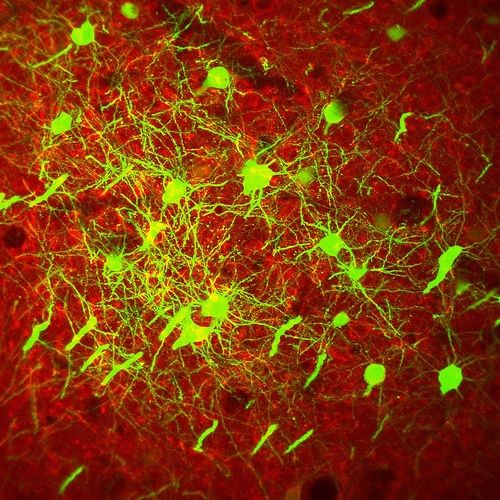
\includegraphics[scale=.3]{./images/NeuroNet.jpg}}
\hspace*{.2in}
\raisebox{-0.5\height}{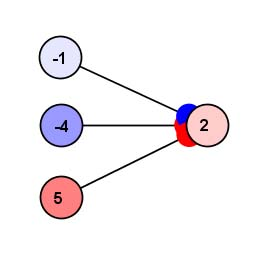
\includegraphics[scale=.5]{./images/Simple3.jpg}}
\caption[Left: Mark Miller, Nelson Lab, Brandeis University. Licensed Under: CC BY-ND; Right: Simbrain screenshot.]{Left: A biological neural network. Right: A simple artificial neural network built in Simbrain, with three nodes connecting to another node via three weights.}
\label{introNets}
\end{figure}

Neural networks can be made to do many fascinating things. They can, for example, drive cars, forecast weather patterns, recognize faces in images, and play the game Go at championship levels. Recently, they have become eerily good at producing human-level written text and images (see the discussion of GPT-3 in chapter \extref{ch_supervised_recurrent} or search the web for images produced by Dall-E). They have been used to model the brain at all of its levels, from individual neurons up to the entire brain. They have been used to model cognition in all of its forms, including memory, perception, categorization, language, and attention. In this chapter, we give a general introduction to neural networks, and survey some of these different ways they are used.

\section{Structure of Neural Networks}\label{structureNets}

In figure \ref{nodesWeights} a simple neural network is shown with some of its parts labeled. In this section, we review the parts of neural networks (nodes and weights), the way they can be structured (their topology), and the relationship between a network and its environment. In each case, bear in mind that what precisely the concepts mean depends on the type of model we are dealing with.\footnote{Neural networks can be used for engineering, to model the brain, or to model the mind. These different uses are discussed in section \ref{typesOfResearch}. Depending on the way a network is being used, the way its parts are interpreted differs, as we'll see.} 

\begin{figure}[h]
\centering
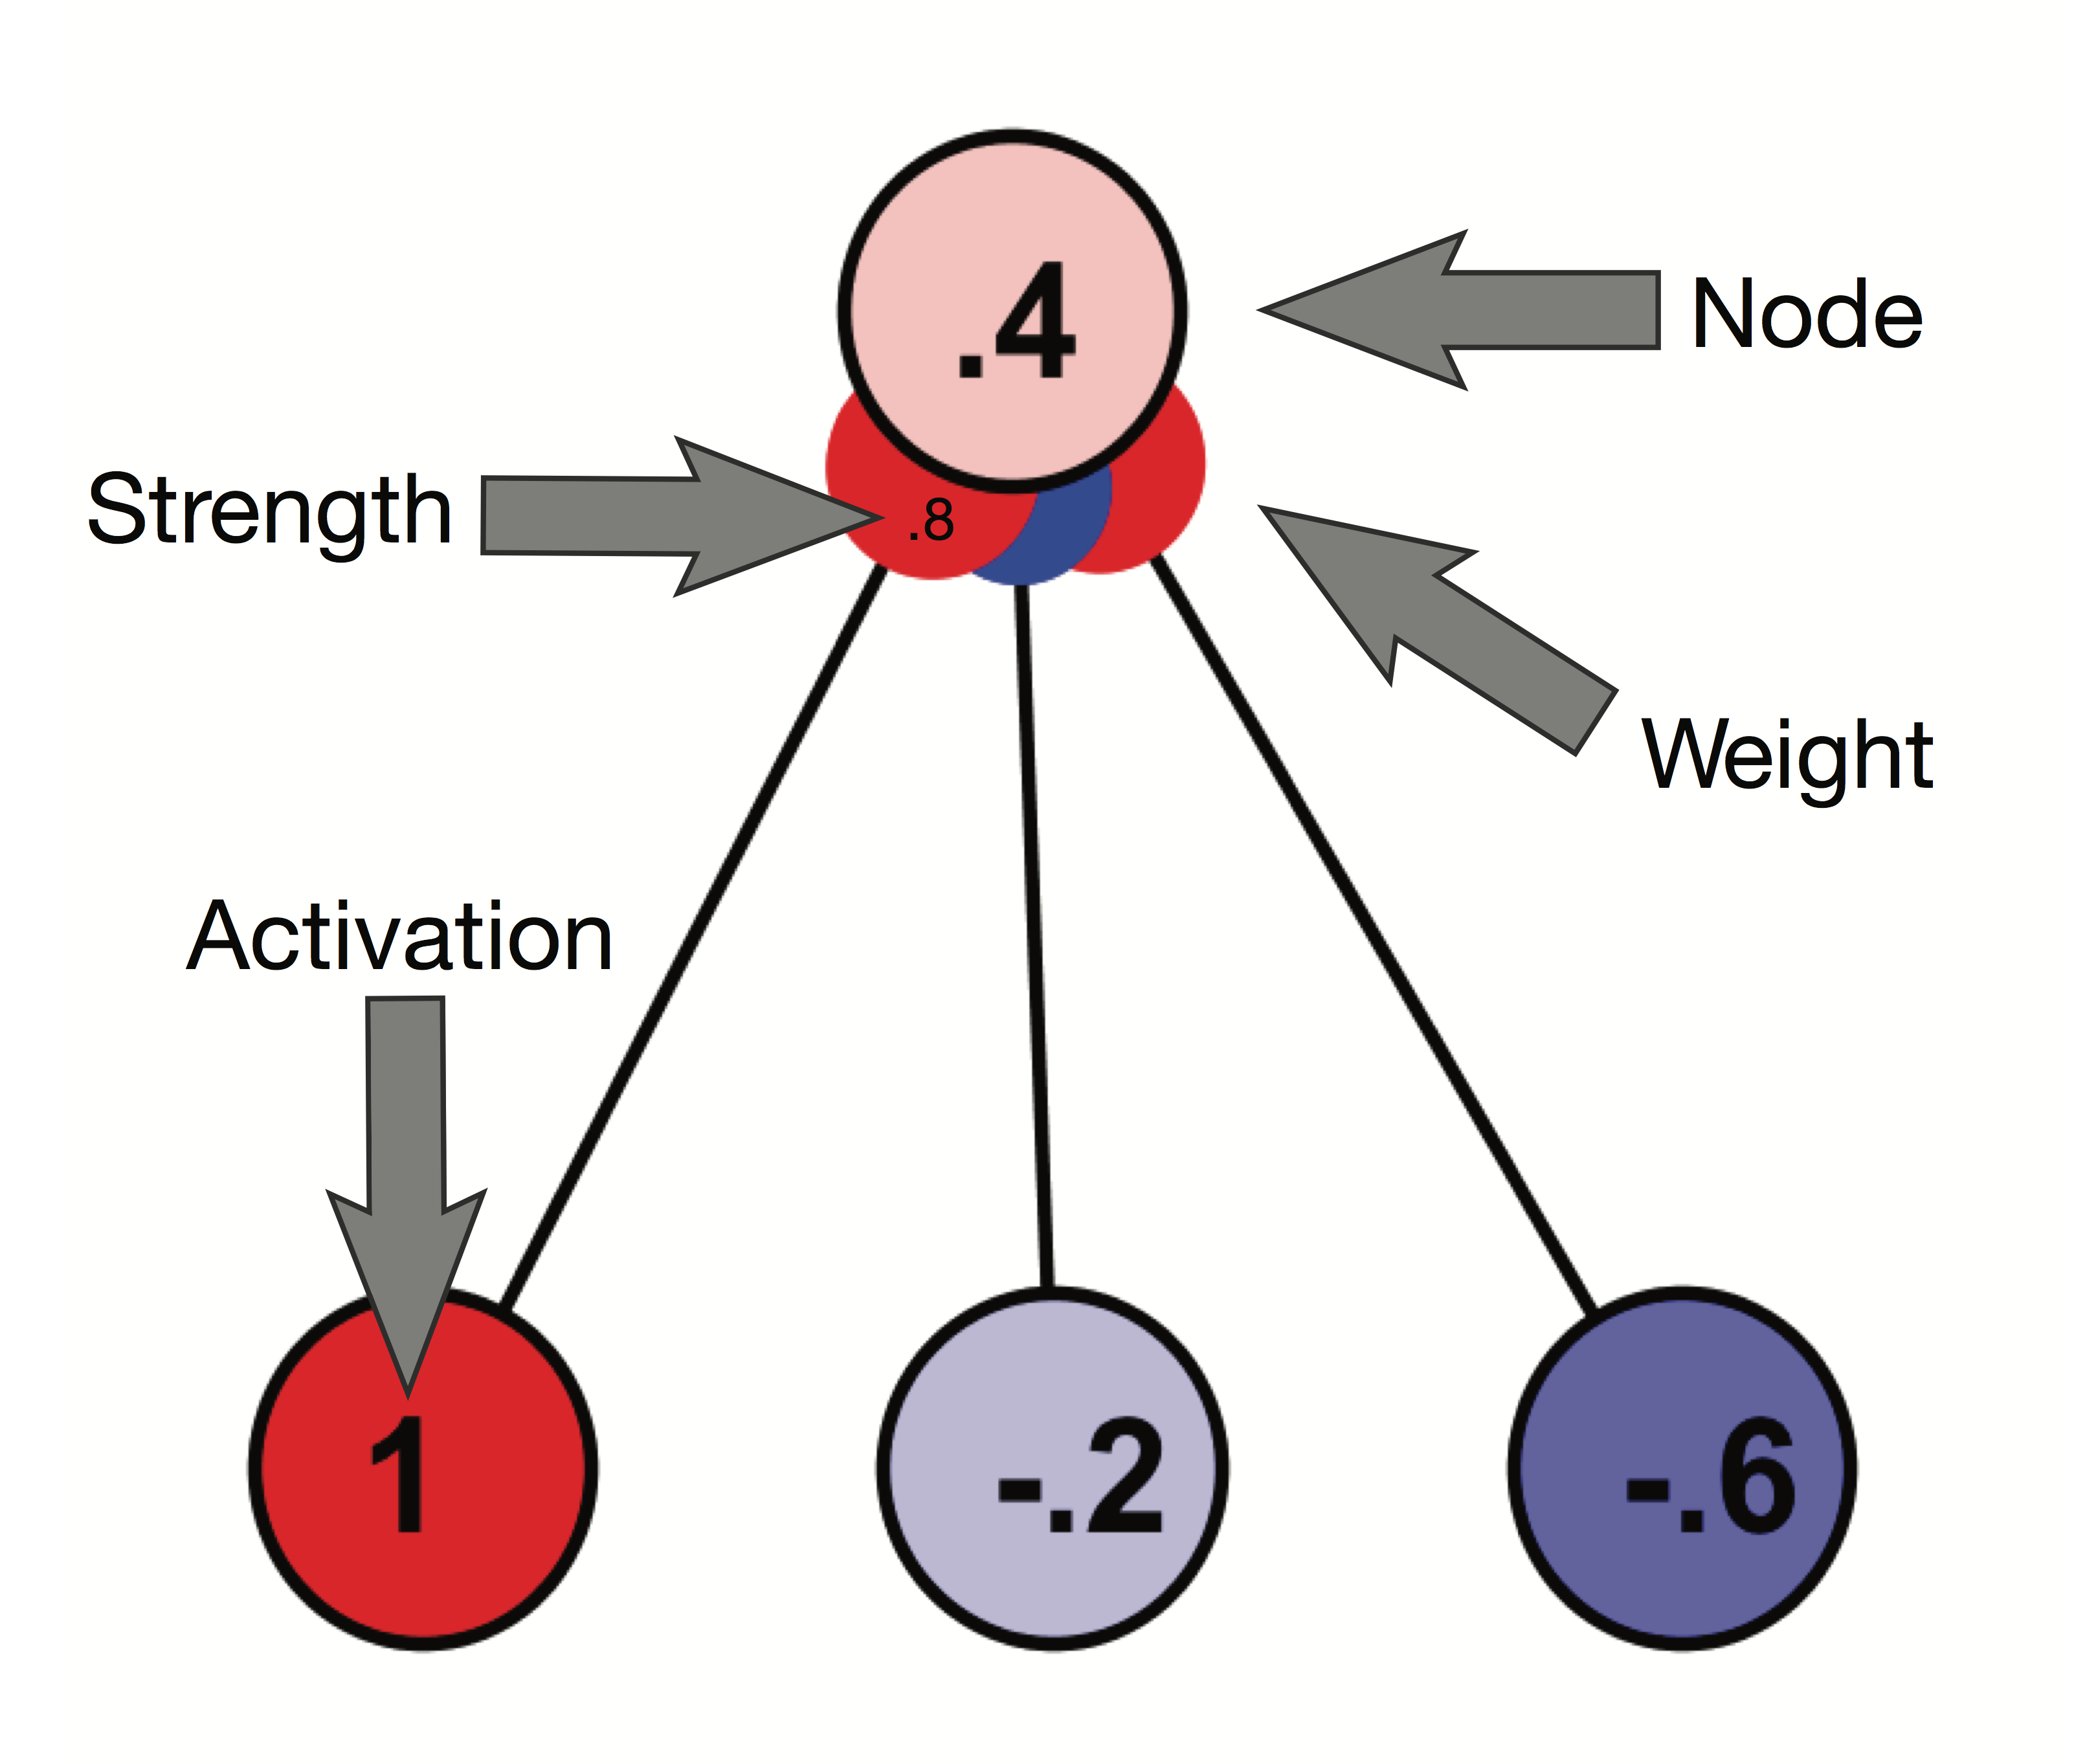
\includegraphics[scale=.2]{./images/labelledNet.png}
\caption[Simbrain screenshot with additional elements added by Pamela Payne.]{Nodes and their activations; weights and their strengths.}
\label{nodesWeights}
\end{figure}

In the figure, a circle with a number in it is an artificial neuron or \glossary{node} (nodes are also referred to as ``units'').\footnote{Sometimes, when the context makes it clear that we are talking about an artificial neural network, terms like ``neuron'' and ``synapse'' are used to mean artificial neuron (i.e. node) or artificial synapse (i.e. weight).}  The number inside a circle corresponds to that node's \glossary{activation}. In Simbrain, red corresponds to an ``active'' neuron (activation greater than 0), and how deep the red is corresponds to how close the activation is to its maximum value. Blue corresponds to an ``inhibited'' neuron (activation less than 0), and how deep the blue is corresponds to how close the activation is to its minimum value. White corresponds to an inactive neuron (activation equals 0). In a computational neuroscience model, these activations might represent the firing rate or membrane potential of a real neuron. In a psychological model, the number might represent the presence of an item in working memory, or the strength of an unconscious belief. As we will see, there is a great deal of variance in what concepts such as activation are taken to mean.
%In computational neuroscience, the numbers represent real properties of neurons and synapses. For example, in some models activation represents a firing rate (number of spikes per second), and in other models it represents a voltage. Weight strength in such models represents the efficacy of a synapse in transmitting information from one neuron to another. In connectionist models of psychological data, the interpretation of activation and weight strength is more abstract. Node activations are sometimes taken to represent the overall activity of a whole population of neurons in some region of the brain, something abstract like the ``strength of a hypothesis'', and they are sometimes simply taken to be hidden variables that have no biological significance whatsoever. \footnote{As McLelland, Rummelhart, and Hinton put it: ``These models assume that information processing takes place through the interactions of a large number of simple processing elements called units, each sending excitatory and inhibitory signals to other units. In some cases, the units stand for possible hypotheses about such things as the letters in a particular display or the syntactic roles of the words in a particular sentence. In these cases, the activations stand roughly for the strengths associated with the different possible hypotheses, and the interconnections among the units stand for the constraints the system knows to exist between the hypotheses. In other cases the units stand for possible goals and actions... and the connections relate goals to subgoals, subgoals to actions, and actions to muscle movements. In still other cases, units stand not for particular hypotheses or goals, but for aspects of these things'' \cite{mcclelland1986appeal}. Or again, as Sejnowski and Rosenberg say: ``The processing units in a network model share some of the properties of real neurons, but they need not be identified with processing at the level of single neurons. For example, a processing unit might be identified with a group of neurons, such as a column of neurons'' (Sejnowski and Rosenberg, p. 146) \cite{sejnowski1987parallel}.}
%  From Cohen et. al on Fear: "Processing units: Simple, nonlinear summing devices can be used as a first approximation of the behavior of populations of real neurons that redundantly code for the same piece of information."
% Perhaps the best discussion of this issues is in Smolensky PTC. (Around table 1)

The lines with filled disks at the end of them are artificial synaptic connections or \glossary{weight}s. These correspond to connections between nodes, which control how activation flows through a network. The weights have a value, a \glossary{strength}. The larger the absolute value of a weight strength, the ``stronger'' it is.  Thus, to strengthen a weight is to increase its absolute value, and to weaken it is to reduce its absolute value.  Stronger weights are shown as larger disks in Simbrain. The actual weight strength can be seen by hovering over the weights or double clicking on them.  As activation flows through a network, the weights with a positive strength (the red weights in Simbrain) tend to enhance activation, and the weights with a negative strength (the blue weights) tend to reduce activation.\footnote{For more details on the graphic representation see \url{http://www.simbrain.net/Documentation/docs/Pages/Network/visualConventions.html}.} In neuroscience terms, these correspond to excitatory and inhibitory synapses. As you play with simulations in Simbrain and study the chapters to come, you will begin to get a feel for how different kinds of weights have different kinds of impacts on the flow of activation in a network. What weight strength represents depends on what kind of model we are dealing with. In a computational neuroscience model, it would represent \glossary{synaptic efficacy}--roughly speaking the impact a pre-synaptic neuron can have on a post-synaptic neuron after the pre-synaptic neuron fires an action potential. In a connectionist or psychological model, the strength might represent an association between concepts. In a machine learning model, there might be no direct interpretation of weight strengths at all: they are mere parameters in a statistical model that does something useful, like recognize faces in images.

Node activations change in accordance with \emph{activation rules} (discussed in ch. \extref{ch_act_functions}),  and weight strengths change in accordance with \emph{learning rules} (discussed in several chapters, including chapters \extref{ch_unsupervised} and  \extref{ch_supervised_ff}). 

In some models a node can also produce a \glossary{spike}, which is a discrete event that corresponds to the action potential of a neuron.\footnote{A spike is represented in Simbrain by a node and all its outgoing connections turning yellow. For an illustration of a spiking node and how it looks in Simbrain, see \url{http://www.simbrain.net/Documentation/docs/Pages/Network/neuron.html}.}  Spiking neurons have their own rules and structures, which we discuss in ch. \extref{ch_spiking}.

Nodes and weights are the basic parts of a neural network. Together, they form a network structure or mathematically, a graph\footnote{\url{https://en.wikipedia.org/wiki/Graph_(discrete_mathematics)}.} where the nodes correspond to vertices, and the weights correspond to edges.\footnote{A neural network is a special type of graph: a vertex-labeled, edge-labeled, directed graph. This means that the edges between nodes have a direction (the graph is \emph{directed}), and that numbers are associated with the vertices and edges (it is \emph{vertex-labeled} and \emph{edge-labeled}).}  The graph-structure formed by a network's nodes and weights is the network's \glossary{topology}. Neural network topologies fall into one of two rough types shown in Fig. \ref{nn_types}: feed-forward and recurrent. 

A  \glossary{feed-forward network} is a sequence of \emph{layers} of unconnected neurons stacked on top of each other such that each layer is fully connected to the next one in the sequence (each node in one layer sends a connection to every node in the next layer).\footnote{\label{acyclic} In graph-theoretic terms, such a network is a directed, acyclic, multipartite graph. It is is \emph{acyclic} because there are no \emph{cycles}; there is is no way to ``move'' from one vertex back to itself along a sequence of vertices connected by edges. It is \emph{multi-partite} because the vertices can be partitioned into \emph{independent sets} (layers), within which none of the vertices are connected. When such a network is not fully-connected from one layer to the next, it is still often referred to as ``feed-forward''. In some cases weights skip over a layer (e.g. go straight from input to output despite the presence of a hidden layer) and again, since activity will still flow ``forward'', this will be referred to as a feed-forward network.}  Activity in this kind of network flows from an \emph{input layer} through a (possibly empty) set of \emph{hidden layers}, and then to an \emph{output layer}.\footnote{Sometimes a distinction is made between \emph{node layers} and \emph{weight layers}. The network in Fig. \ref{nn_types} has three node layers (labelled ``input layer'', ``hidden layer'', and ``output layer'') and two weight layers (labelled ``1-2'' and ``2-3''). To make matters even more confusing sometimes people don't count the input layer as a node layer. In Simbrain, node and weight layers are both represented as groups, indicated by the yellow interaction boxes: \url{http://www.simbrain.net/Documentation/docs/Pages/Network/groups.html}. When used without qualification, we use the term ``layer'' to mean ``node layer''.}   In a feed-forward network activity  simply passes through; when the input nodes are activated and the network is updated, the activation flows from layer to layer and is then erased. Feed-forward networks are often classifiers: an input (which might represent an image, or a smell) passes through the layers of the network and the output activations then represent a way of classifying the input (saying who is in the image, or what object is being smelled).
% Promote the discussion of node vs. weight layer to main text
%The effects of any input to the network on the network will be completely erased after $n$ iterations where $n$ is the number of layers.
% The graph representing weights from one layer to layer to the next in a feed-forward network is an example of a bipartite graph.

In a \glossary{recurrent network}, the nodes are interconnected in such a way that activity can flow in repeating cycles.\footnote{In graph-theoretic terms, this is a cyclic graph, which contains at least one cycle. Recall from footnote \ref{acyclic} that a directed cycle is a sequence of directed edges that begin and end at the same vertex. That is, starting at one node of such a network, we can ``travel'' from one node to another via the connections and end up back where we started. }   Recurrent networks display complex dynamical behaviors that don't occur in feed-forward networks since activity in the network cannot always ``leave'' the network. Most biological neural networks are recurrent. In machine learning, recurrent networks can be used to simulate dynamical processes, for example,  to mimic human speech, or create artificial music.
% Any input to such a network \emph{influences} rather than dictates the network's future states, which are determined by both the current input and the current state of the network (itself a product of previous inputs and/or the network's own internal dynamics). 

\begin{figure}[h]
\centering
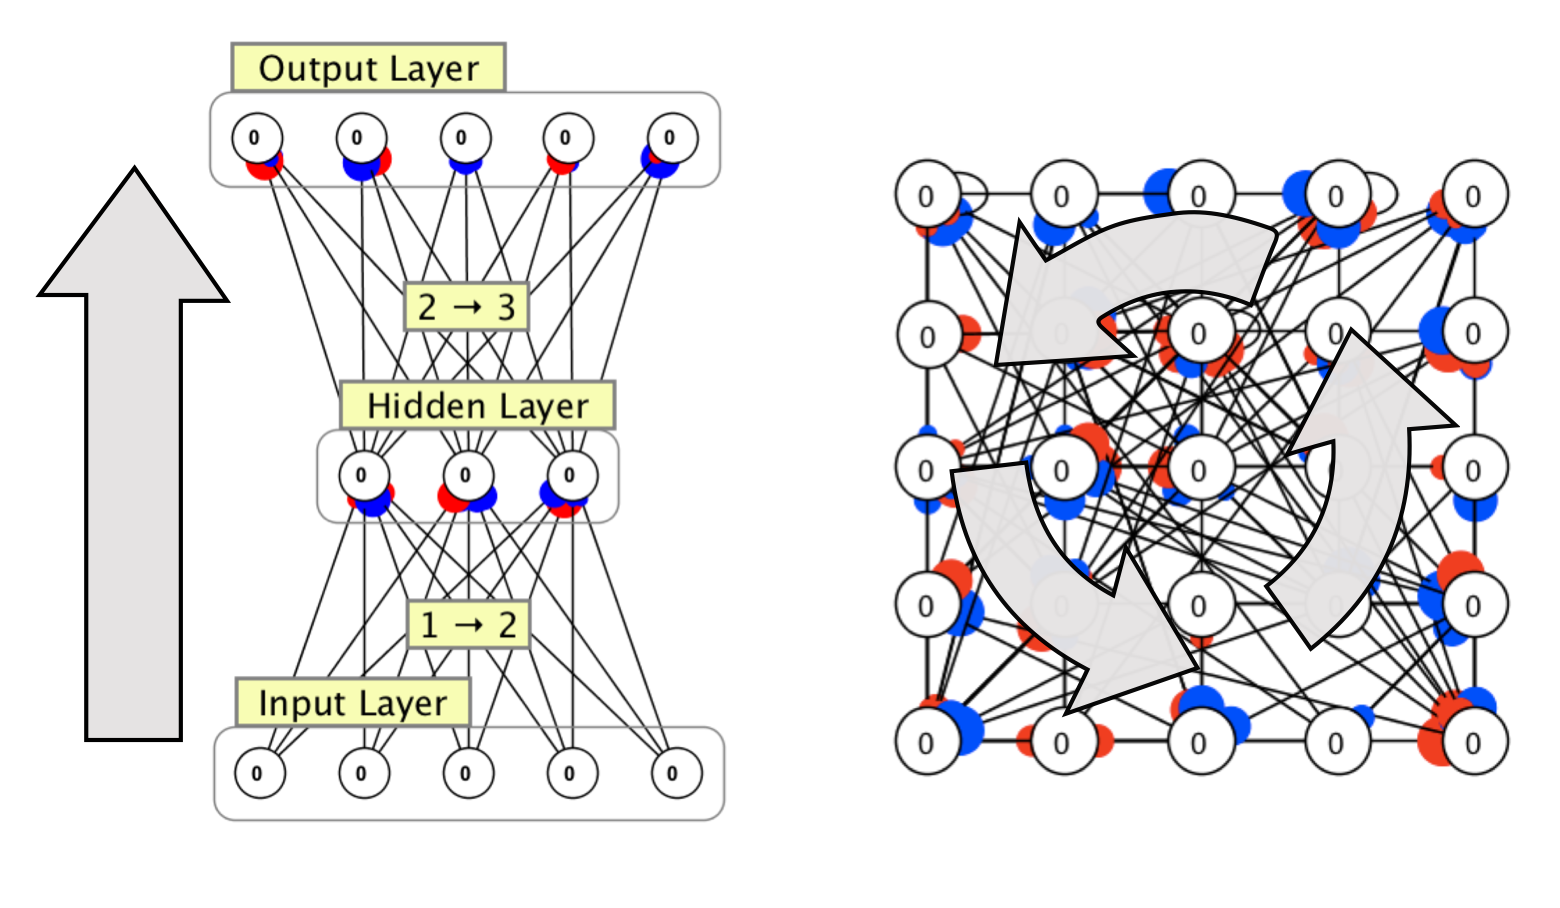
\includegraphics[scale=.7]{./images/NeuralNetTypes.png}
\caption[Simbrain screenshots with additional elements added by Pamela Payne.]{Feed-forward network (left) and recurrent network (right). Gray arrows give a sense of how activation flows through them.}
\label{nn_types}
\end{figure}

There are other kinds of architecture beyond the ones just mentioned. An especially popular architecture since the 2010s has been the \glossary{deep network} architecture, which involves many layers of neurons and weights (some of them arranged into stacks or ``tensors'' at a given level), often using a special type of layer called a ``convolutional'' layer, which scans over its input to produce outputs. An example of a deep network is shown in figure \ref{deep_net}. Deep networks are discussed in more detail in section \extref{deepNets}. Note that networks like this are so large, that we can't represent each node and weight separately. Instead node layers containing thousands of nodes (or more) and weight layers containing tens of thousands  of weights (or more)  are shown as sheets or lines. This is something we have to get used to: there are different ways of drawing neural network diagrams. 

\begin{figure}[h]
\centering
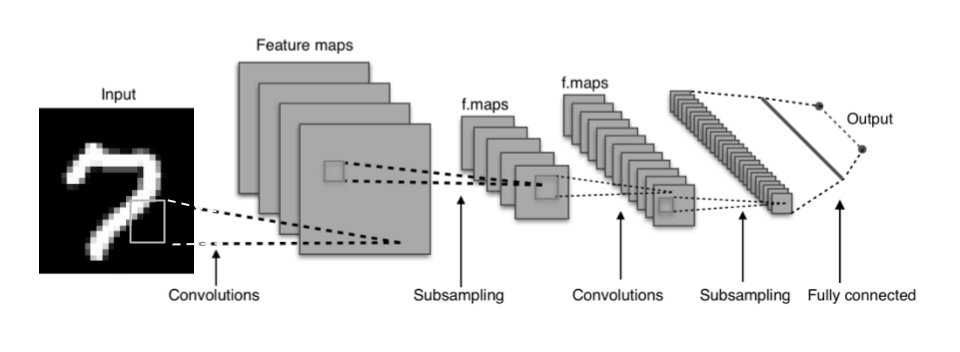
\includegraphics[scale=.45]{./images/deepNet.png}
\caption[Adapted from a creative commons image by Aphex34 at \url{https://commons.wikimedia.org/wiki/File:Typical_cnn.png} ]{A deep neural network, trained to recognize images. The convolutional layers scan over the inputs they are linked to. }
\label{deep_net}
\end{figure}

Networks almost always exist in some kind of  \glossary{environment}, which gathers inputs for a network and receives its outputs. For example, a neural network that converts speech to text can be connected to audio sensors, like the microphone on your phone. It can take audio in, convert it to text, and send the result out via the speakers. However, by far the most common way a neural network is linked to inputs and outputs, especially when building and testing them, is via tables of data. Training and testing datasets are discussed at length in chapter \extref{ch_data_science}. In Simbrain, we will also link neural networks to virtual environments. Figure \ref{nn_environment} shows how some of these configurations might look. Couplings between a network and an environment occur at special nodes:  an \glossary{input node}  is influenced by the environment, while an  \glossary{output node} exerts an influence on the environment. In figure \ref{nn_types} (left), for example, the input nodes are the nodes in the input layer, and the output nodes are the nodes in the output layer.\footnote{Information on how to couple nodes to an environment in a Simbrain simulation, and thus treat them as input or output nodes, is available here: \url{http://www.simbrain.net/Documentation/docs/Pages/Workspace/Couplings.html}.} 
%The recurrent network on the right might also have input and output nodes (or nodes that are both at once), but this is not directly visible in that figure.

\begin{figure}[h]
\centering
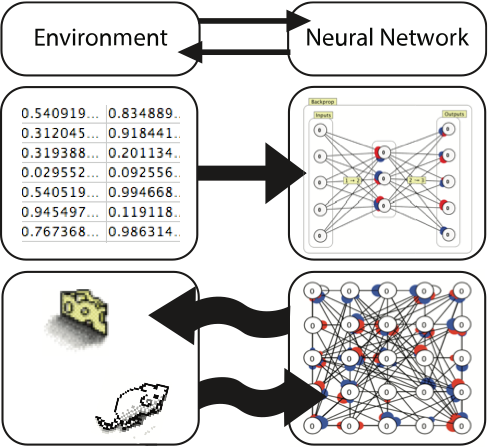
\includegraphics[scale=.7]{./images/nn_environment.png}
\caption[Pamela Payne.]{The relationship between a neural network and an environment. An ``environment'' is often something as simple as a table of values (middle row). However it can also be something more complex, like a virtual world (bottom row).}
\label{nn_environment}
\end{figure}

\section{Computation in Neural Networks}\label{intro_comp_nn}

We've seen what the parts of a neural network are, and learned some basic concepts relating to their structure. We now turn to a few concrete examples in Simbrain that give a sense of how computation works in neural networks: how they channel information, and how they can actually perform interesting tasks. 

\begin{figure}[h]
\centering
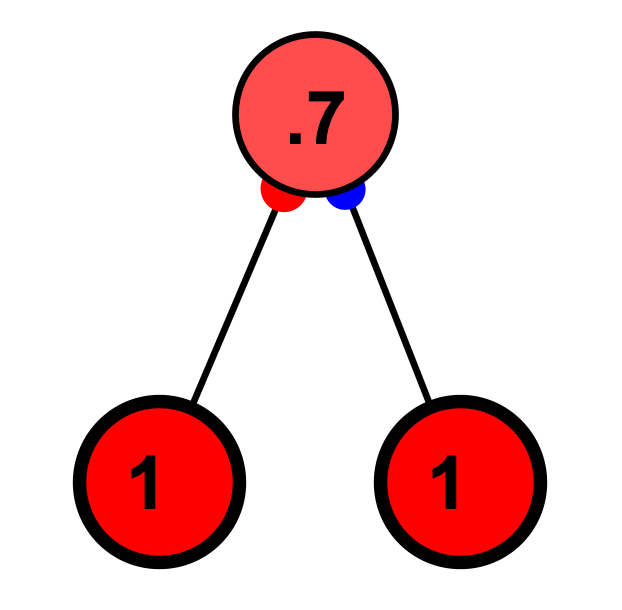
\includegraphics[scale=.4]{./images/2-1_ff.png}
\caption[Simbrain screenshot.]{Simple feed-forward network with clamped inputs. By adjusting the weight strengths, we can make the output activation be whatever we want.}
\label{2NodeSimpleFF}
\end{figure}

To begin with, how do neural networks ``channel information''? The mathematical details are not too difficult, but for now we are developing basic intuitions.\footnote{This is an example of a linear activation function. The output is obtained by multiplying each input activation times the strength of the intervening weight. See chapter \extref{ch_act_functions}. In this case the weight strengths are $.8$ and $-.1$, and so the output is $1 \times .8 + 1 \times (-.1) = .7$. Since the input activations are 1, the output in this case is just the sum of the two weights: $.8 -.1 = .7$.} Consider the network shown in figure \ref{2NodeSimpleFF}: it's a simple feed-forward network with two node layers (an input and output layer) and one weight layer. The inputs are \glossary{clamped node}s, and are thus represented with a bold-faced outline. This means they will not change their value when we update the network. How is the activation of the output node determined? Let us briefly assume that all activations are positive, as they are in the figure.\footnote{In fact, in some contexts negative activations are taken to be unrealistic or problematic. Neuron spiking rates are always positive, for example. In recent years the ``relu'' activation function, which disallows negative activations, has become extremely popular in deep learning.}  Assuming all activations are positive, we can think of outputs as being computed in the following way:
\begin{enumerate}
\item  Positive weights (red disks) increase outputs. They ``heat things up.'' As they are strengthened, the output gets larger.
\item  Negative weights (blue disks) decrease outputs. They ``cool things down.'' As they are strengthened (as their absolute value is increased), the output gets smaller.
\end{enumerate}
The two weights are like two knobs that we can turn up or down, that we can use to \emph{tune} the output. Suppose we want the output to be some other value besides $.7$, like $.9$. To do this, we could strengthen the positive weight a little bit so that it makes the output larger.  We could also weaken the negative weight so that it decreases the output less. Or both. In a similar way, to reduce the output to $.5$, we could either weaken the positive weight or strengthen the negative weight. In doing so, we are tuning the weights up and down to get the output we want.  Most of the theory of neural networks is about automatically tuning weights and other parameters to get useful flows of activation. 
% Of course this example is simplified. In general nodes do additional computations, like placing a cap on how big or small the activation can get, adding decay terms, or introducing thresholds where only if there is enough input does the node turn on. 

With this background in hand, let's move to an example that shows how computation in neural networks differs from computation in a standard digital computer. In both neural networks and digital computers, information is processed, but the \emph{way} it is processed differs. Consider the simulation  {\em threeObjectsDist.zip}.  A screen shot of the network, which we call the ``three object detector'',  is shown in Fig. \ref{3ObjectClassifier}.\footnote{A video about the three object detector (including information about how to load it) is available at \url{https://youtu.be/yYzUmcPaurI?t=380}. } The three object detector has a feed-forward topology with three nodes in the input layer, seven nodes in the hidden layer, and three nodes in the output layer. The example is not meant to model the brain directly. It is more abstract:  it classifies inputs in a  brain-\emph{like} way. It takes a pattern of inputs, and transforms those inputs through a network of connections. This is similar to the way information processing occurs in the brain. But it is not a realistic simulation of a brain circuit (as we will see, it is a ``connectionist network'' as opposed to a ``computational neuroscience'' model).
% See warehoused philosophyofconnectionism.txt, which contains information on the link to symbolic AI.

In this example we also see how a network can be linked to a virtual environment. The mouse in the simulated world on the right of figure \ref{3ObjectClassifier} is hooked up to this network. When the mouse is moved around, the activation in the input nodes changes. This simulates the way odor molecules impact the inner lining of the nose, causing sensory neurons to fire at different levels. So the input layer is a kind of simulated nose. The job of this network is to distinguish the three objects on the basis of those sensory inputs. Depending on which object the mouse is near, a different output node should be activated. This is called a ``classification task''.

\begin{figure}[h]
\centering
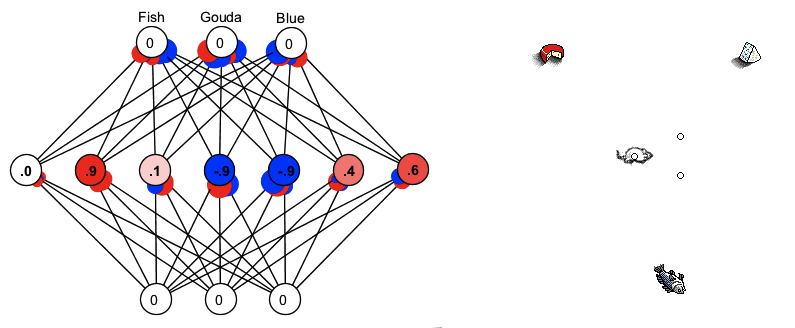
\includegraphics[scale=.4]{./images/3Node_World.png}
\caption[Simbrain screenshot.]{Simple feed-forward network that recognizes three objects.}
\label{3ObjectClassifier}
\end{figure}
% Possibly put in Beer Categorical perception picture here for an example of mixed

We can use this example to illustrate certain  general properties of computation in neural networks, which can be contrasted with classical computation in a digital computer.\footnote{Of course, neural network simulations are usually run on a traditional computer performing classical computations. But that is a convenient way of implementing the formal structure of a neural network. These implementation can still take advantage of all the special properties of neural networks. Moreover, it is in fact possible to implement neural networks directly on hardware.} In a classical computer discrete symbols (comprised of strings of 0s and 1s, or ``bits'') are operated on by rules, in a sequential manner. Bits of information are placed in registers on a computer's central processing unit (CPU), and logical rules in the CPU's instruction set are applied to these bits. Computers are hand-programmed to do useful things. The inside of a CPU and the memory systems on a computer are carefully controlled environments. They do not do well with noisy signals or damage. Computation in a neural network is  different. Neural computation is not based on sequential, rule-based operations on bits, but on parallel operations where patterns of node activations are transformed by weight strengths.\footnote{We can often represent this as a transformation of \emph{activation vectors} (lists of activation values) by \emph{weight matrices} (tables representing weight strengths). So, while the basic formalism of classical computation is logic,  the basic formalism of neural networks is \emph{linear algebra}, which we study in chapter \extref{ch_linear_algebra}.}    Neural networks are also more tolerant of noisy signals and damage than digital computers are. And they are not programmed, in the way a computer is, but are trained, in something like the way a human child is.

Let's use the three object detector simulation to consider some of these contrasts in more detail. 

Networks are \emph{trained}, not programmed. We show the network what we want it to do, and it learns to do it. In the three object detector, for example, here is (very roughly) what happened: we put the mouse near the fish, and said, ``when you smell something like this, fire your first node.''  Then we did the same thing with the Gouda and blue cheese. Each time we exposed the network to an object, we used the ``backprop'' algorithm (discussed in a chapter \extref{ch_supervised}) to adjust the network's weights. At first the network made mistakes, but with each exposure to an object the weights were changed a little, and over time it got better and better at recognizing cheese, in something like the way humans and animals gradually get better at doing things with training. This is called \glossary{supervised learning}, since we know the correct output for each input and can tell the network exactly what output it should produce for any given input.  The great thing about this is that once we've trained the network on some data, \glossary{generalization} is possible, where it can deal with new data it's never been exposed to before. We can train a network to respond to a bunch of cheese we have available, and on that basis it can recognize new pieces of cheese it's never seen before. This is part of what makes neural networks--both the one's used in your cell phones but also the one that is inside your skull right now helping you read this--so valuable. After a bit of training and learning, they can be let loose in the world and deal with brand new situations.

This isn't the only way neural networks can be trained. For example, neural networks can also learn by a system of rewards and punishments (reinforcement learning). They can also learn without any kind of training signal or reinforcement, simply by picking up on the statistical structure of their environment (\glossary{unsupervised learning}).\footnote{Much more rarely, the weights are hand-crafted, as in the IAC networks later in this chapter. But that is the exception that proves the rule. IAC networks are great at illustrating activation dynamics, but highly unusual in that the weight strengths are not learned from data, but are hand-set by a human.}

Second, neural networks work in \emph{parallel}. Whereas digital computers normally do things one at a time, in a sequence, neural networks do a lot of things  \emph{at the same time}. To see the difference this can make, consider a simple problem: finding which of ten cups has a jelly bean under it. A serial approach would lift each cup up, one at a time, until the jelly bean was found. A parallel approach would lift all ten cups up at once. Neural networks operate like this, processing information in all the nodes, all at once, all the time. This is easy to see  in the three object detector simulation: when you run the simulation and drag the mouse around, the activations of all the nodes will change based on the new inputs in parallel. 
% Qualifiers about serial on a parallel computer, etc.

% Do a pass on the footnote below before re-introducing it
%\footnote{Parallel computation is clearly faster. So, why not do everything in parallel? The answer, roughly, is that the whole theory of digital computation assumes a core level of serial processing. To implement a basic algorithm assumes that things happen in a well-ordered fashion. Techniques for parallel computation exist, and are emerging as an important area of computer science, but in those cases tasks are merely broken down into sub-tasks which are each run in serial side-by-side. However not every algorithm is ammenable to this sort of decomposition (many tasks require the full evaulation of some portion of the task before another step in the task can be started) and to make matters worse the physical limitations of computer hardware as it pertains to memory management and allocation prevents even those which are ammenable from achieving peak theoretical performance. With a few (rare) exceptions 8 processing elements (PEs) working on a task in parallel will never complete a task 8x faster than a single PE for these reasons. However this sort of parallelism isn't the same kind of parallelism as what we find in living neural networks. In computer-world we have synchronous, discrete parallelism; in neuro-world we have asynchronous, continuous parallelism. A great many neurons act asynchrnously in parallel each as its own mini-PE sending and receiving signals from sensory inputs and other neurons such that what exactly each neuron is responding to or what its doing can be quite nebulous. The sorts of representation of information that the brain can support are fuzzy and fleeting, but robust. This tends to be excellent for recognizing objects, catching a fly-ball, learning to move, making analogies or being creative, but in general is poorly suited to (for instance) fast, accurate, memory-intensive numerical computation. This fuzziness is perfect for our very fuzzy world, but in the realms math and logic can be prone to mistakes. 

 %Moreover, serial computers are fast these days. For example, the computer I'm writing this on performs several billion operations per second. With numbers like those we can tolerate the processing slow-down due to serial processing.On the other hand, massively parallel processors like the brain are messy, they make mistakes. They are not as good as computers at performing, e.g., complex mathematical computations or looking up names in an index. And they are made of relatively slow materials. Neurons fire at most 200 times per second. They are orders of magnitude slower then the transistors on this computer. In order to solve problems in a reasonable time frame the brain operates in parallel: every neuron is always doing its own thing. The trade-off is in accuracy: the brain is a kind of messy computer, which doesn't always do the same thing twice. But given the wet, biological stuff we're made of, it works well enough.}

% More details on what to do in sim
Third, neural networks \emph{gracefully degrade} when they are damaged (this is also called ``fault tolerance''). They are not brittle in the way a digital computer is. You can start deleting the weights of a neural network and it will still work reasonably well. You can try doing this on the three object detector!   In a  similar way, if you lose a few neurons and /or synapses, you will be just fine. Of course, if you lose enough neurons and synapses it will start to show, but it will happen gradually and  proportionally to the damage. It is in this sense that neural networks degrade ``gracefully.''\footnote{This is related to the fact that they operate in parallel rather than serial. A neural network has lots of redundant wiring which can compensate for damage.}  A digital computer, by contrast, is not designed to continue functioning if its components are damaged. Pluck a micro-chip out of the motherboard, or snip a few wires, and there's a good chance your computer will stop working altogether. 

Fourth, neural networks are good at \emph{handling noisy inputs}. Digital computers don't like noisy input: they respond only to clean, precise inputs. Anyone who has worked with computers has some understanding of this. To get through a company's phone tree you have to enter just the right sequence of numbers--no mistakes allowed!  But show me the same flower ten times, and I will see it as the same flower, even though the input to my brain is changing slightly (the lighting changes, things in my retina change, the whole process is noisy). You can see this in the Simbrain simulation by dragging the mouse around. Notice that even while the inputs change slightly the network continues to recognize which object it's looking at.

\section{Types of Neural Network Research}\label{typesOfResearch}

In practice, neural networks are used in two main ways: (1) as engineering tools, and (2) as scientific models.
% Definition of scientific model and some reference to literature on the topic

When neural networks are used as engineering tools, they are used to do useful things, like recognize faces in photographs or convert speech to text. Neural networks used for engineering do not have to be psychologically or neurally realistic, they just have to work well. In fact, it is preferable if they are \emph{better} than humans, making fewer mistakes than we do.

Neural networks used for scientific modeling should be neurally or psychologically realistic; they should accurately describe how the brain and the mind work. A neural network model of human memory, for example, should remember (and forget) things in the same way humans do in experiments. This second use of neural networks--as models of the mind and brain--itself subdivides into several subcategories, depending on what specifically is being simulated. Neural networks are sometimes used to understand the brain (in the field of ``computational neuroscience''), sometimes to understand mind and behavior (this is sometimes called ``connectionism''), and sometimes to understand both brain and mind simultaneously.
 
\subsection{Engineering uses of neural networks}\label{machineLearning}

% Other engineering uses: 
% Fausett section 1.3
% Wiki deep  learning page

Neural networks in engineering are tools to solve problems. They are used as classifiers, controllers, signal processors and other components, alongside many other types of engineering tools. Neural networks in this area are used as statistical models (one kind of  \glossary{machine learning} model). These models are good at  finding patterns in complex and noisy data. Remember, neural networks are trained, not programmed, making them well suited to tasks where there is no obvious way to mathematically determine the relationship between a set of inputs and a set of outputs.

% As two workers in the field put it:
%\begin{quote}
%The most natural application areas for [neural networks] are obviously tasks in which appropriate transformations from certain inputs to certain outputs should be established, but the transformations cannot be discovered analytically due to a variety of reasons. Therefore it is no wonder that the most successful applications of the [neural networks] can be found in the areas of machine vision, pattern recognition, motor control, signal processing, etc., where such input to output transformations dominate the problem solving \cite{heikkonen1999building}.
%\end{quote}
%Engineers who use neural networks for these purposes don't care about how the brain works or how humans think: they want to make a machine that works. A neural-network based rice cooker (like the ``Zojirushi neuro-fuzzy rice cooker''; google it!) should make good rice, whether it cooks like humans do or not. 

\begin{figure}[h]
\centering
\raisebox{-0.5\height}{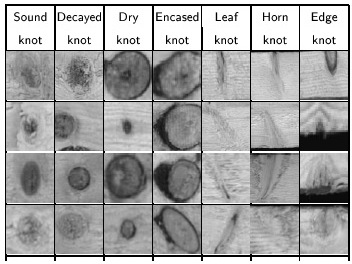
\includegraphics[scale=.4]{./images/wood_network_stimuli.jpg}}
\hspace*{.2in}
\raisebox{-0.5\height}{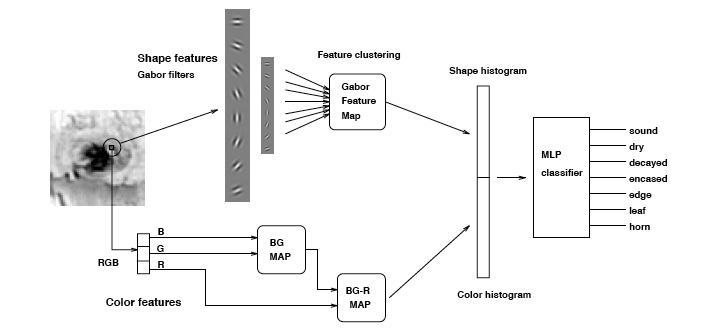
\includegraphics[scale=.3]{./images/wood_network_flowchart.jpg}}
\caption[From Heikkonen et al., 1999 \cite{heikkonen1999building}. Licensed Under CC BY-NC]{Left: Sample inputs to the knot classification network. Right: The knot classification system. The neural network is labelled ``MLP.''}
\label{knotNet}
\end{figure}

Here is an example from the late 1990s. A lumber yard in Finland had to classify pieces of wood, identifying 30 different kinds of knot in images of lumber. Some examples are shown on the left side of figure \ref{knotNet}. A human can classify these knots, but it is time-consuming, expensive, and error-prone (look at how subtle some of the differences are between the different ``dry knots''). It is also hard to program a computer to classify these knots according to explicit rules. Thus, neural networks were used, and they outperformed humans. A neural network trained on samples like the one shown have about 90\% accuracy in this process, compared with 70-80\% accuracy for humans. The neural network is shown in the figure. It is  buried inside the system, the ``MLP classifier'' towards the right (``MLP'' means ``multi-layer-perceptron,'' which is a feed-forward network trained by backpropogation. It is  similar to the 3-object detector above). This system takes a picture of a piece of wood, does some pre-processing on the resulting pixel image, and then summarizes features and colors of that image as a list of numbers, which is fed to the neural network as input. The neural network transforms these numbers into another list of numbers, which describe how decayed, burnt, dry, round, and so forth each sample is. This is a \emph{feature vector}. This feature vector can then be used to classify the knot \cite{heikkonen1999building}.
% Note on pre-processing and forward ref to learning chapter, and data wrangling.

\subsection{Computational neuroscience}\label{computationalNeuroscience}

\glossary{Computational neuroscience} uses computational methods to answer questions related to neuroscience. Computational neuroscience spans many levels, from the micro-scale of cell membranes to the macro-scale of the human brain as a whole (see Fig. \ref{compNeuro}). It is a highly multidisciplinary field, encompassing biology, neuroscience, psychopharmacology, cognitive science, complexity science, psychology, and even physics, depending on the context. 

\begin{figure}[h]
\centering
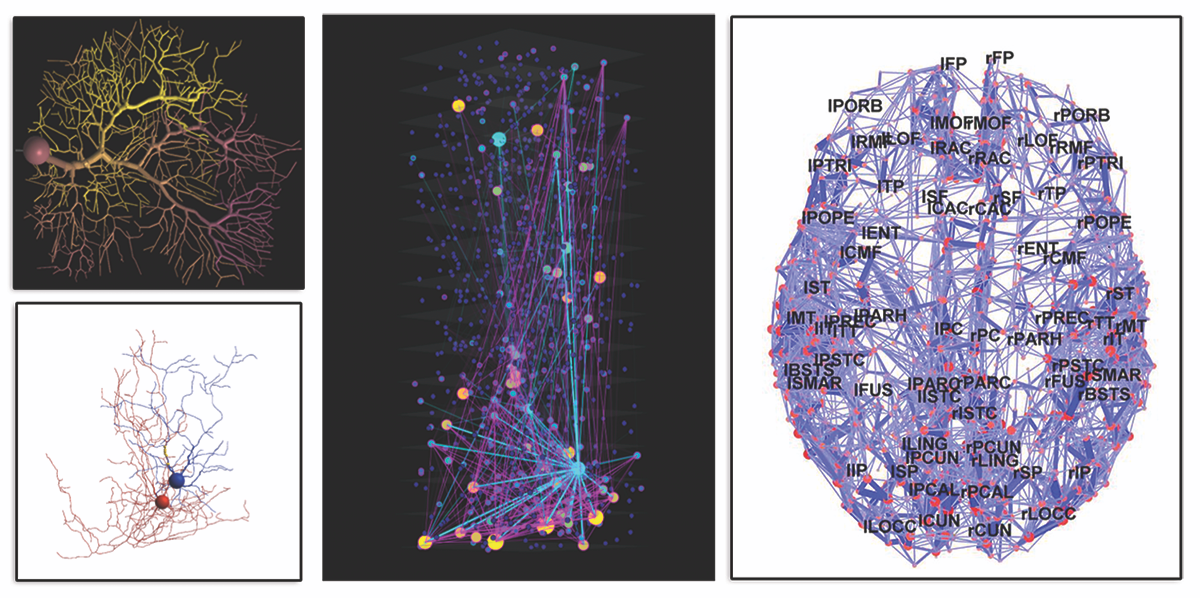
\includegraphics[width=0.8\textwidth]{./images/3typesmodels.png}
\caption[Layout by Pamela Payne. Top Left: ; Bottom Left: ; Middle: Screenshot by Zach Tosi ; Right: From Hagmann et al., 2008 \cite{hagmann2008mapping}, Licensed Under CC BY]{Micro, meso, and macro-level models in computational neuroscience. Left: micro-level models of individual neurons. Middle: meso-level model of a network of several thousand neurons. Right: macro-level model of neuronal connections spread out through the entire brain.}
\label{compNeuro}
\end{figure}
% http://medicalxpress.com/news/2013-11-entire-brain-brainbow-ii-technology.html
% https://upload.wikimedia.org/wikipedia/commons/thumb/e/ef/Network_representation_of_brain_connectivity.JPG/1280px-Network_representation_of_brain_connectivity.JPG

\emph{Micro-scale} models in computational neuroscience study individual neurons or even individual parts of neurons, like the receptors that are studded in the cell membrane to let charged particles in and out of a cell (these are models of ``receptor kinetics''). Models at this level often study the details of how charge flows through the tree-like structures of a neuron's dendrites and axons, and can accurately describe the behavior of individual neurons in a laboratory dish (``in vitro'') when they are injected with current from small electrodes. Models at this level often attempt to answer questions that are physiological or pharmacological in nature like the effect of neuromodulators on the low level dynamics of a neuron, or how new receptors are created or new dendritic spines are grown. These models are largely below the level of what is visible in a single Simbrain node.

\emph{Macro-scale} models in computational neuroscience describe the behavior of large groups of thousands to millions of neurons  and the connections between them. Oftentimes these models approximate the activity of thousands of neurons or even whole brain areas as the activity of a single higher level node.\footnote{As an example, see \url{https://www.ncbi.nlm.nih.gov/pubmed/21511044} \cite{cabral2011role}} These models can accurately describe the spatio-temporal organization of patterns of neural activity measured using brain imaging techniques like fMRI. In a Simbrain network simulation of this kind each node would represent the aggregate activity of thousands to millions of neurons and the whole network could represent the behavior of the entire brain. Models of this type are usually concerned with questions which are psychological or behavioral in nature. For instance the functional relationships between brain regions have been shown to be different in patients with schizophrenia resulting in a different overall graph structure of the functional connectivity between brain regions \cite{bullmore2009complex}. Often work at this level ``bleeds over'' into the realm of general neuroscience.

In this book we mostly focus on the \emph{meso-scale} (or ``middle''-scale) of computational neuroscience, between the micro and macro-levels. Whereas micro-scale models focus on individual neurons or their parts, meso-scale models focus on networks of \emph{hundreds to thousands} (or more) of interconnected neurons. And whereas each node in a macro-level model \emph{approximates} the activity of large group of real neurons, each of the simulated neurons in a meso-level simulation  corresponds to a real neuron. Thus, a meso-level simulation containing 1000 artificial neurons is a direct simulation of a biological neural network containing 1000 real neurons. The emphasis is on discerning governing principles and dynamical phenomena associated with these networks. Meso-level models in computational neuroscience have been implemented in Simbrain (e.g. the middle image in Fig. \ref{compNeuro}). 

The model neurons and synapses used in these simulations  are  more complex than the simple nodes and weights described above in Sect. \ref{structureNets},  since they are designed to mimic the electrochemical properties of real nerve cells. Most neuron models in computational neuroscience are governed by equations acting on variables which represent specific electrochemical attributes of living neurons. Synapses have temporal delays and their signals have duration. Network models in computational neuroscience tend to be comprised of \emph{spiking neurons} (neuron models which produce and propagate signals via action potentials) embedded in complex \emph{recurrent} networks. We cover the special properties of these model neurons and networks in chapter \extref{ch_spiking}.\footnote{In contrast to the micro-scale, which is (broadly) concerned with physiology, and the macro scale, which is often concerned with psychology, the meso-scale concerns itself with questions like: How do networks of interconnected neurons represent information? Can we replicate synaptic connectivity using plasticity rules? How does information processing emerge from the interactions of neurons embedded in a neural network?'  Meso-scale models often attempt to understand formalisms that describe observations of groups of neurons (e.g. slices of brain tissue) with explanations of those observations using models of detailed low level processes at the micro-scale. It is known that when neurons fire in particular temporal sequences the synapses connecting them will become stronger or weaker depending upon that sequence. A micro-scale model might concern itself with how new receptors are created, or new spines are grown. A meso-scale model will only concern itself with the function translating that temporal sequence into a change in synaptic strength.} 

Very roughly, the focus of computational neuroscience at these  three scales can be thought of as follows:
Neuron Dynamics $\rightarrow$ Network Dynamics $\rightarrow$ Brain Dynamics

\subsection{Connectionism}\label{connectionism}

% See Talking Nets 259, 283, 274
% Maybe talk more about semantic memory and semantic network models, and contrast with other types of memory (many will not have taken intro cog-sci courses)
The use of neural networks as cognitive models, which behave in the same way humans and animals do, but without concern for neural realism, is sometimes called \glossary{connectionism}.\footnote{Not everyone using the term ``connectionism'' in this way, but it is a fairly standard usage. A more precise phrase would be ``connectionist model of a cognitive process''.}  In connectionist models, there is no direct effort to understand the brain. The focus is on modeling some aspect of human or animal behavior using nodes and weights. Such models  are usually meant to {\em suggest} how a given task is accomplished by the brain---they are ``neurally plausible''---but they do not directly model the underlying neuroscience.

As an example, consider the ``IAC'' or ``Interactive Activation and Competition'' network. A famous example of an IAC network is McClelland's model of knowledge of two fictional 1950s gangs, the Jets and Sharks from {\em West Side Story} \cite{mcclelland1981retrieving}.\footnote{For a video overview of this network in Simbrain, see \url{https://www.youtube.com/watch?v=Nw3TEDfugLs}.}

\begin{figure}[h]
\centering
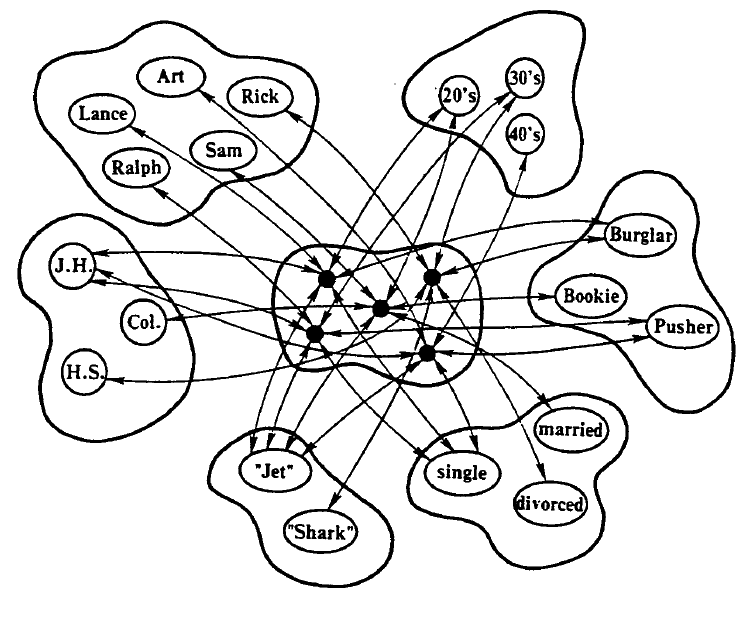
\includegraphics[scale=.3]{./images/IAC_JetsSharks.png}
\caption[From McClelland and Rumelhart, 1989 \cite{mcclelland1989explorations}.]{A fragment of the Jets and Sharks model. Nodes in this model don't represent neural activity, but activation of concepts in semantic memory.}
\label{iac}
\end{figure}

% Maybe just go full Simbrain. Change the example and make clear that it can be done in many ways.
% Make the object pool / property pool distinction more central, and give more examples.
% In a sense a model of the ventral stream, but not the dorsal stream. No ``embodied'' memory captured, no dorsal stream, and no retrieval mechanisms. Maybe refer to publications about actual semantic memory. BUT don't want to emphasize neuro too much so a balance.
% A good contrast to supervised, unsupervised, and generalization. A strange case where we hand-tune the weights. Note there is NO learning in these model. So the concepts of supervised and unsupervised don't apply. It is hand tuned. 

An IAC model is organized into pools of nodes. In Fig. \ref{iac}, there are 7 pools of nodes. These pools of nodes are used to model the internal concepts of a person who knows about these two gangs. The pools represent different  traits:  age, education level, marital status,  job, etc. The central pool is a pool of ``instance nodes'' or ``object nodes'', shown as black disks, which correspond to individual people. Each person is associated with a node. The other pools correspond to properties of these people: their name, job, age, and gang affiliation. The nodes in each pool inhibit each other, which produces a \emph{winner-take-all} structure. As the simulation runs, the activation of one node in each pool will tend to dominate the others. Notice that the topology of this network is recurrent, and as a result the network has dynamics: when we run it, activation starts to spread from one node to another over time. In fact, these have also been called \emph{spreading activation} networks \cite{mcclelland1981retrieving}. 

The IAC network models general features of human semantic memory, like the ability to retrieve attributes of a person based on their name. If the Lance node is activated and the simulation is run, activation will spread through the recurrent network, and after a while the Jets node, 20s node, Junior high education node, and burglar node will have the highest activations. This is like asking ``Tell me about Lance?'' and being told about him. The network can also model our ability to describe the properties of a group of people. If the Jets node is activated and the network is run, the standard characteristics of the Jets will light up: they tend to be in their 20s, with a junior high school education, and single. This is like asking ``Tell me about the Jets?'' and being told about that group. The network can also model our ability to identify people who match a specific description. If the 20s node and the junior-high education node are activated, then the name nodes for Lance, Jim, John, and George all light up. This is like asking ``Who is in their 20s with a junior high education?'' and being told ``Well, that could be Lance, Jim, John, or George.''
%\footnote{Notice that the nodes and connections in this model don't correspond to actual neurons or synapses. The IAC network captures the empiricist theory (associated with John Locke and David Hume) that  human knowledge is encoded in abstract associations between ideas. Node activations correspond to the presence of an item in thought or memory, or what the empiricist philosophers called \emph{ideas}. If the ``Lance'' node is active, that corresponds to a person thinking about Lance. Connections between nodes correspond to \emph{associations} between ideas. The whole network of connections represents our overall knowledge about something, in this case, two gangs. When one node  is activated and the network is run, all the associated nodes are activated. Over time all the ideas associated with the original idea should be activated \cite{mcclelland1981retrieving}. Nodes and weights represent ideas and associations in an abstract brain-like way without modeling neuroscience directly.} \cite{mcclelland1981retrieving}

Though IAC networks are models of semantic memory, and are brain-like (spreading activation and winner-take-all types of dynamics do occur in the brain), they are \emph{not} models of the brain, they do not capture any details of human neuroscience, or have nodes whose activation corresponds to activity in specific parts of the brain.

\begin{figure}[h]
\centering
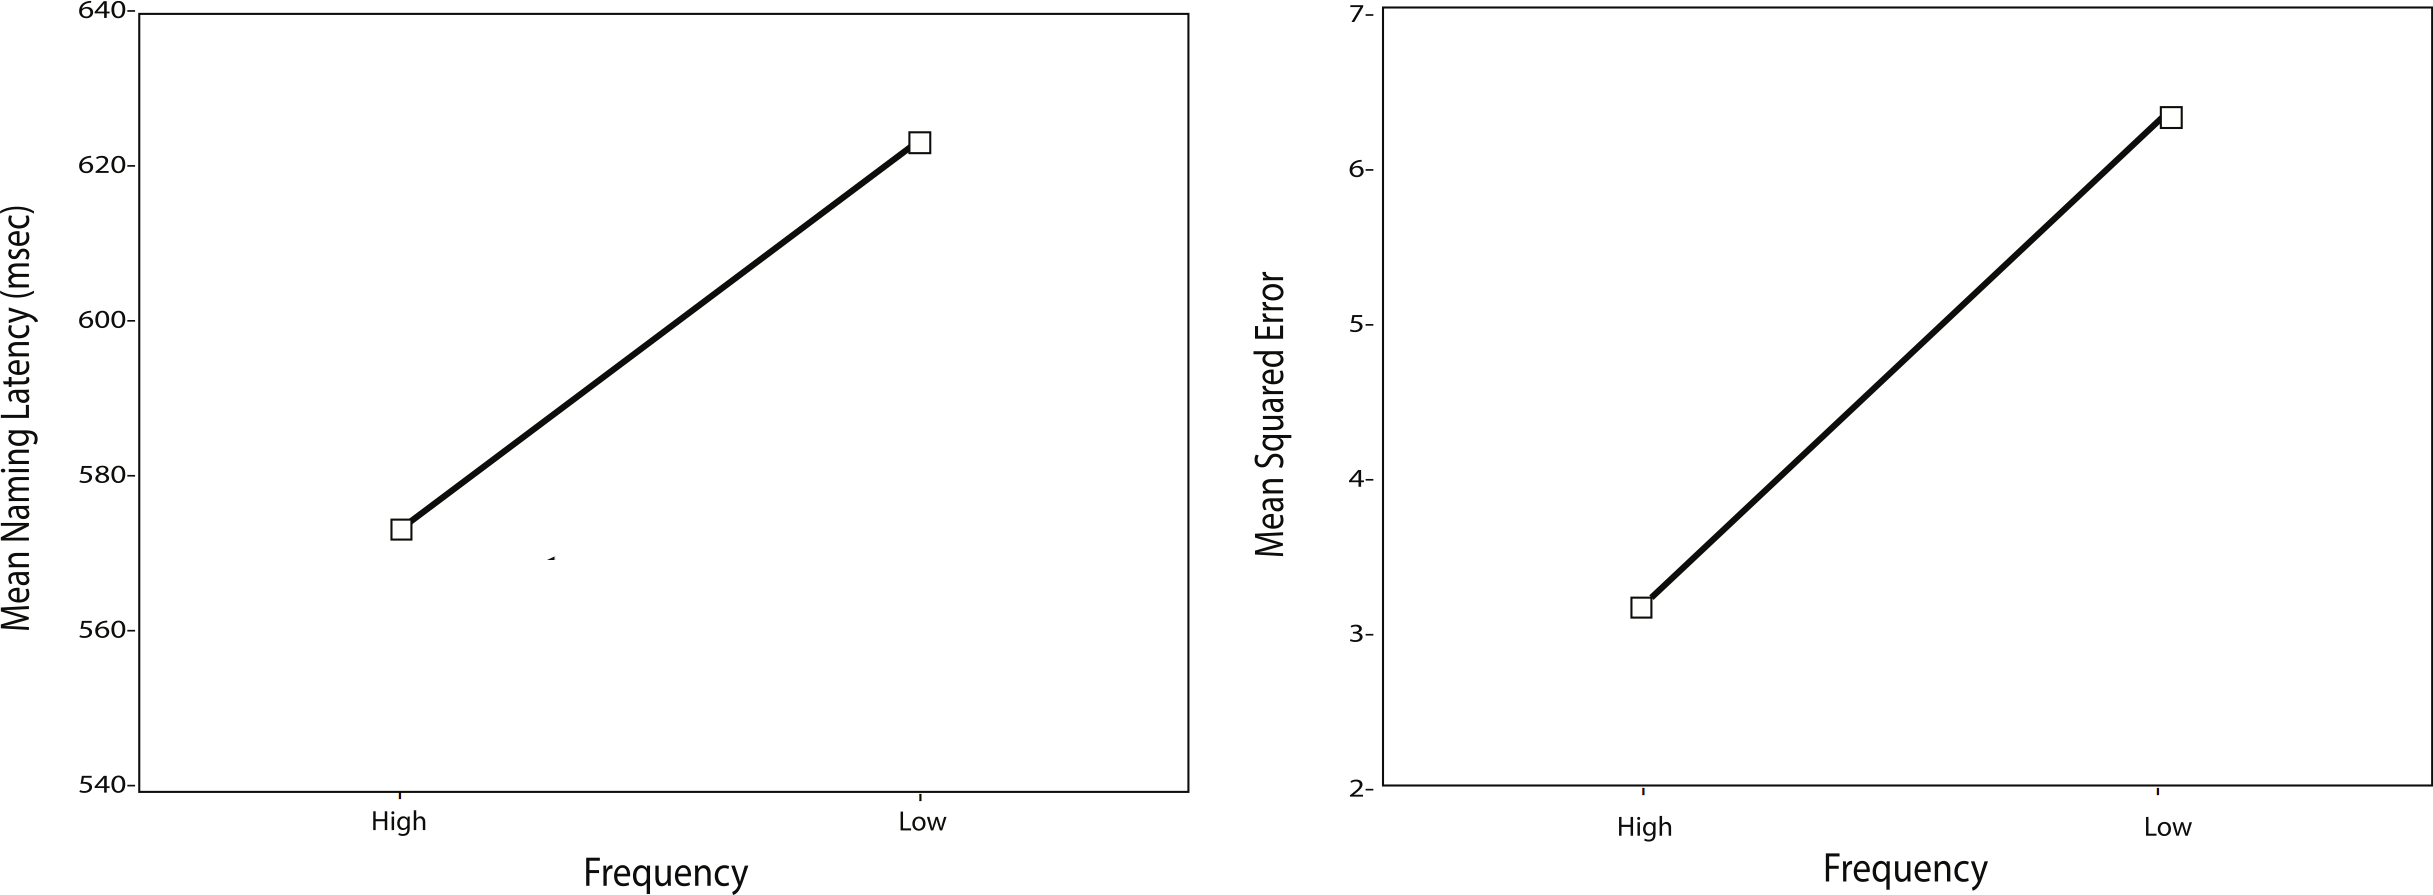
\includegraphics[width=0.8\textwidth]{./images/seidWordNet_Data3.png}
\caption[From McClelland and Seidenberg, 1989 \cite{seidenberg1989distributed}. Redrawn by Pamela Payne.]{Data associated with Seidenberg and McClelland (1989)'s reading model. Human data are on the left, neural network data are on the right. Humans pronounce high frequency words more quickly than low-frequency words. The neural network makes fewer errors on high frequency than low-frequency words.}
\label{regularityData}
\end{figure}
 
% This has become so short it might be time to get remove it, keep things simple. One main example per section. As it is it gets a bit lost. If used, take the opportunity to talk about error in a bit more detail.
The IAC network is a qualitative model of human memory. Other connectionist simulations are more quantitative. For example, Seidenberg and McLelland  modeled childrens' reaction times in reading words aloud. The network is a variant on a feed-forward network, similar to the network on the left side of figure \ref{nn_types}. It has  more nodes: 400 input units, which represent written words, and 460 output units, which represent spoken words. It was trained to pronounce all one-syllable words in English using a method called ``backpropogation'' (chapter \extref{ch_supervised}). This simulation models  the \emph{word frequency effect}. Words that occur frequently in language (like ``the'') are pronounced more quickly than words that occur infrequently (like ``rake'').
%\footnote{\label{exceptionsVsRegular}The model also captures the ``frequency-regularity interaction'', whereby words that have regular pronunciation patterns (e.g. ``gave'' or ``must''), are pronounced faster than exception words (e.g. ``have''  or ``pint''). However, this regularity effect only occurs for infrequent words. This is also shown in the figure: in each graph the upper curve with the open squares show exception words; the lower curves with filled triangles show regular words.}  

Human data showing this effect are on the left side of Fig. \ref{regularityData}. Humans pronounce high frequency words more quickly than  low frequency words (the $y$-axis shows latency, or length of time to pronounce the word; lower values mean faster times). The neural network data on the right  was generated by counting how many mistakes the network made for low and high frequency words \cite{seidenberg1989distributed}. When you line the two graphs up next to each other, they look the same. This suggests that the way the model reads is similar to the way humans read: both the neural network model and humans are better at reading more common words.
%\footnote{ Many questions come up here, and you might not be satisfied (in fact, this model was involved in a kind of war between connectionist and non-connectionist models of  reading). The main thing  to emphasize here is that the model is supposed to capture some kind of human, behavioral data.}

\subsection{Mixed and intermediate cases}

Both distinctions discussed in this section can be difficult to apply. It can be difficult to know whether a neural network model is being used as an engineering or a scientific model. It can also be hard to say whether a scientific model is being used to simulate the brain (computational neuroscience), or cognition and behavior (connectionism). Some models do both at once.

The first distinction, between engineering and scientific uses of neural networks, can be confusing because the two usages have been historically intertwined. Some neural networks that originated as scientific models later got used as engineering tools. Sometimes the reverse happens: an engineering tool ends up being useful as a scientific model. Deep networks provide a striking example of these back and forths. As we discuss in chapters \extref{ch_history} and  \extref{ch_neuro}, deep neural networks  were originally used as models of vision in the 1970s. These later turned out to be excellent tools for pattern recognition, when they were used to recognize digits on envelopes, leading to the deep learning revolution of the 2010s. These new and improved deep networks turned out to be useful in computational neuroscience as a way to understand the human visual system. So, a neural network that started off in science, then got used for engineering, and then later that tool then got adapted back to science!

A good rule of thumb when considering how to classify a neural network is to ask: ``What is the neural network being used for? As a tool, or as a scientific model?''\footnote{A more advanced way to ask this question is to ask: how are the node activations and weight strengths being interpreted? Are they merely parameters in statistical models, or are they supposed to capture something real about neurons, or about concepts and their relations?} Even then it can be tricky. For example, consider the following title of a journal article: ``Use of Neural Networks in Brain SPECT to Diagnose Alzheimer's Disease'' \cite{page1996use}. At first, this sounds like it might be about a computational neuroscience or connectionist model, since it mentions the brain and Alzheimer's. However, the article is actually about how neural networks can be used to determine whether a person has Alzheimer's. The neural network is not being used as a model of the brain or any cognitive processes, but rather as an engineering tool to help diagnose Alzheimer's disease based on brain images. If we ask: ``What is the neural network they made being used for?'', the answer is to build a better diagnostic tool, \emph{not} as a model of schizophrenia. So it's really an engineering usage of a neural network, rather than a scientific model.

As far as the distinction within scientific modeling between computational neuroscience and connectionist models, here too there are difficult cases, mainly because many people who use neural network models are interested in \emph{both} how the brain works \emph{and} how cognition works, and of course, how the two are related. Thus, there are increasingly many models that attempt to capture both neural and psychological data, as was noted in the discussion of macro-level computational neuroscience above. 

For example, models in \glossary{computational cognitive neuroscience} attempt to capture psychological and behavioral data while simultaneously paying attention to neural details. This type of model captures various aspects of cognition (e.g. visual attention, semantic and episodic memory, priming, familiarity, and cognitive control), using groups of neurons that are explicitly associated with specific brain circuits. Many researchers hope that over time computer models of brain and behavior will converge, and that future models will increasingly capture both neural and behavioral data, and thereby reveal how the dynamics of the brain give rise to the dynamics of cognition.\footnote{Examples of researchers and research groups working in this area include the work of Randy O'Reilly and his colleagues (\url{https://grey.colorado.edu/CompCogNeuro/index.php/CCNBook/Main}), Stephen Grossberg's work which began in the 1960s (\url{https://en.wikipedia.org/wiki/Stephen_Grossberg}), and the work of Chris Eliasmith and his colleagues (\url{https://uwaterloo.ca/centre-for-theoretical-neuroscience/people-profiles/chris-eliasmith}).} Some examples of this type of model are shown in figure \ref{ccn}.

% Emergent ref since I have a spaun ref?
\begin{figure}[h]
\centering
\raisebox{-0.5\height}{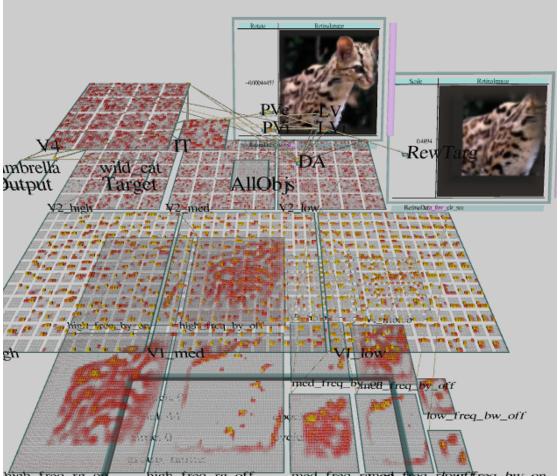
\includegraphics[scale=.3]{./images/EmergentScreenshot.png}}
\hspace*{.4in}
\raisebox{-0.5\height}{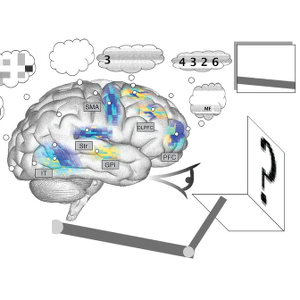
\includegraphics[scale=.6]{./images/spaun.png}}
\caption[Left: From \url{https://grey.colorado.edu/emergent/index.php/File:Screenshot_vision.png}; Right: Spaun screenshot. Cf. \cite{eliasmith2012large}.]{(Left) An Emergent simulation of visual processing, with labels indicating which brain areas each group of nodes represents. (Right) A Nengo simulation of the human ability to retrace a visually perceived number.}
\label{ccn}
\end{figure}

 From this standpoint, computational neuroscience and connectionism are two ends of a continuum or spectrum. We have computational neuroscience at one end, and connectionism at the other. All through the middle of this spectrum are models that try to model both biological data and psychological data at the same time. The goal is to understand how the circuits of the brain produce all the wealth and complexity of observable human and animal behavior. 


%\chapter{Applications of Neural Networks}\label{ch_applications}
\chapterauthor{Jeff Yoshimi, Zo\"e Tosi}{.8,.2}

% See discussion with Pierre on  Jun 12, 2024
% Rep alignment, interpretability, Zipser. Activation patching. Mechanistic interpretability.
% "Every time I fire a linguist, the performance of our system goes up." Apocryphal to Frederic Jelneck as reported by Sven Matty.  Same for neuroscientist, philosopher, whatever, ML and gradient descent seem to just power their way through any attempt to post hoc understand this stuff.

In this chapter we consider how neural networks as models are applied in various areas of engineering and science, with an emphasis on applications to cognitive science, given the scope of the book. One fascinating feature of applications of neural networks, especially in recent years, is how a model that was initially designed for one purpose takes on a completely different meaning in another context. For example, neural networks that were initially used to study the visual system ended up being useful to engineers designing pattern recognition devices. Those pattern recognition devices then became interesting to scientists studying vision. ChatGPT and similar models were designed to provide a useful natural language  interfaces (and to support other features like machine translation), but they perform so well that they have become objects of interest for scientists and theorists.\footnote{It's a strange situation: systems designed by humans are not completely understood by the people who designed them, and so they have become topics of scientific and philosophical inquiry.}

\section{Engineering vs. Scientific applications}

In practice, neural networks are applied in two main ways: (1) as engineering tools, and (2) as scientific models.\footnote{See the discussion of ``standards of intelligence'' in \cite{noelle2022artificial}. Models of idealized intelligence are what we are calling ``engineering'' models here, while psychologically realistic cognitive models are what we are calling ``neural networks as scientific models.''}

When neural networks are used as engineering tools, they are used to do useful things, like recognize faces in photographs or convert speech to text. Neural networks used for engineering do not have to be psychologically or neurally realistic, they just have to work well. In fact, it is preferable if they are \emph{better} than humans, making fewer mistakes than we do.

\begin{figure}[h]
\centering
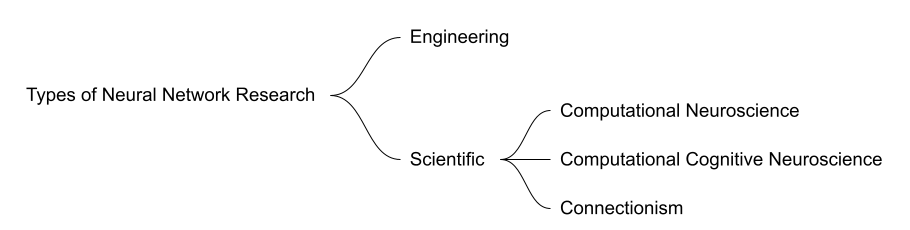
\includegraphics[scale=0.4]{./images/TypesOfNNResearch.png}
\caption[Jeff Yoshimi.]{A taxonomy of types of neural network research, which serves as a guide to this section. Engineering uses (section \ref{machineLearning}) where the goal is to just make something useful, and scientific models where the goal is use neural networks to model the mind (connectionism, section \ref{connectionism}), the brain (computational neuroscience, section \ref{computationalNeuroscience}), or both (computational cognitive neuroscience, section \ref{mixedCases}).}
\label{typesNN}
\end{figure}

Neural networks used for scientific modeling should be neurally or psychologically realistic; they should accurately describe how the brain and the mind work. A neural network model of human memory, for example, should remember (and forget) things in the same way humans do in experiments. This second use of neural networks--as models of the mind and brain--itself subdivides into several subcategories, depending on what specifically is being simulated. Neural networks are sometimes used to understand the brain (in the field of ``computational neuroscience''), sometimes to understand mind and behavior (this is sometimes called ``connectionism''), and sometimes to understand both brain and mind simultaneously. A map of these types of research is in figure \ref{typesNN}. As we will see, this taxonomy is not always so neat, and there are fascinating cases of, for example, engineering neural networks becoming objects of scientific interest.

A good rule of thumb when considering how to classify a neural network model is to ask: ``What is the neural network being used for? As a tool that does something useful, or as a scientific model?''\footnote{A more advanced way to ask this question is to ask: how are the node activations and weight strengths being interpreted? Are they merely parameters in statistical models, or are they supposed to capture something real about neurons, or about concepts and their relations?} Even then it can be tricky. For example, consider the following title of a journal article: ``Use of Neural Networks in Brain SPECT to Diagnose Alzheimer's Disease'' \cite{page1996use}. At first, this sounds like it might be scientific model, since it mentions the brain and Alzheimer's. However, the article is actually about how neural networks can be used to determine whether a person has Alzheimer's. The neural network is not being used as a model of the brain or any cognitive processes, but rather as an engineering tool to help diagnose Alzheimer's disease based on brain images. If we ask: ``What is the neural network they made being used for?'', the answer is to build a better diagnostic tool for Alzheimers. The network is \emph{not} being used a model of Alzheimers. So it's really an engineering usage of a neural network, rather than a scientific model.

\section{Engineering uses of neural networks}\label{machineLearning}

% Other engineering uses: 
% Fausett section 1.3
% Wiki deep  learning page

Neural networks in engineering are tools to solve problems. They are used as classifiers, controllers, signal processors and other components, alongside many other types of engineering tools. In fact, in the contemporary world, many things we take for granted are built on top of neural networks engineered to do useful things. They are at the heart of the current revolution in AI (as of 2023). They recognize voice and images, they generate speech, the generate images and movies, they drive cars, and of course, they can have human-like conversations with us (as with large language models like ChatGPT). They do many of the things humans do, often better than we can, because we can carefully engineer them and train them on such massive datasets.

We will see in later chapters how to systematically classify these different kinds of models, but for now we can focus on a very common case: the use of neural networks to classify objects, which is  one application of  \glossary{machine learning}. Classifiers are good at  finding patterns in complex and noisy data. Remember, neural networks are trained, not programmed, making them well suited to tasks where there is no obvious way to mathematically determine the relationship between a set of inputs and a set of outputs.

% As two workers in the field put it:
%\begin{quote}
%The most natural application areas for [neural networks] are obviously tasks in which appropriate transformations from certain inputs to certain outputs should be established, but the transformations cannot be discovered analytically due to a variety of reasons. Therefore it is no wonder that the most successful applications of the [neural networks] can be found in the areas of machine vision, pattern recognition, motor control, signal processing, etc., where such input to output transformations dominate the problem solving \cite{heikkonen1999building}.
%\end{quote}
%Engineers who use neural networks for these purposes don't care about how the brain works or how humans think: they want to make a machine that works. A neural-network based rice cooker (like the ``Zojirushi neuro-fuzzy rice cooker''; google it!) should make good rice, whether it cooks like humans do or not. 

\begin{figure}[h]
\centering
\raisebox{-0.5\height}{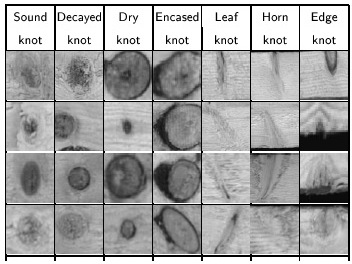
\includegraphics[scale=.4]{./images/wood_network_stimuli.jpg}}
\hspace*{.2in}
\raisebox{-0.5\height}{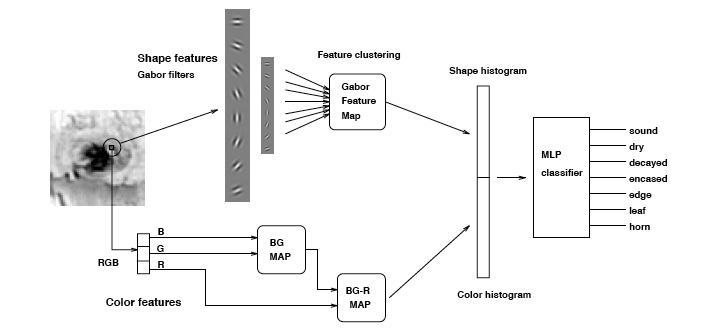
\includegraphics[scale=.3]{./images/wood_network_flowchart.jpg}}
\caption[From Heikkonen et al., 1999 \cite{heikkonen1999building}. Licensed Under CC BY-NC]{Left: Sample inputs to the knot classification network. Right: The knot classification system. The neural network is labelled ``MLP.''}
\label{knotNet}
\end{figure}

Here is an example from the late 1990s. A lumber yard in Finland had to classify pieces of wood, identifying 30 different kinds of knot in images of lumber. Some examples are shown on the left side of figure \ref{knotNet}. A human can classify these knots, but it is time-consuming, expensive, and error-prone (look at how subtle some of the differences are between the different ``dry knots''). It is also hard to program a computer to classify these knots according to explicit rules. Thus, neural networks were used, and they outperformed humans. A neural network trained on samples like the one shown have about 90\% accuracy in this process, compared with 70-80\% accuracy for humans. The neural network is shown in the figure. It is  buried inside the system, the ``MLP classifier'' towards the right (``MLP'' means ``multi-layer-perceptron,'' which is a feed-forward network trained by backpropogation. It is  similar to the 3-object detector above). This system takes a picture of a piece of wood, does some pre-processing on the resulting pixel image, and then summarizes features and colors of that image as a list of numbers, which is fed to the neural network as input. The neural network transforms these numbers into another list of numbers, which describe how decayed, burnt, dry, round, and so forth each sample is. This is a \emph{feature vector}. This feature vector can then be used to classify the knot \cite{heikkonen1999building}.\footnote{Pre-processing is one aspect of data wrangling, which is discussed in chapter \extref{ch_data_science}.  Post-processing also occurs, for example all things that happen in ChatGPT  after the network produces its raw output (for example filtering out inappropriate responses).}
% TODO: Here or above in environment? why here? And make clear processing -> vector -> vector -> post-processing

\section{Computational neuroscience}\label{computationalNeuroscience}

We now turn from neural networks used as engineering tools, to neural networks used as models of the mind and brain.

\glossary{Computational neuroscience} uses computational methods to answer questions related to neuroscience. Computational neuroscience spans many levels, from the micro-scale of cell membranes to the macro-scale of the human brain as a whole (see Fig. \ref{compNeuro}). It is a highly multidisciplinary field, encompassing biology, neuroscience, psychopharmacology, cognitive science, complexity science, psychology, and even physics, depending on the context. 

\begin{figure}[h]
\centering
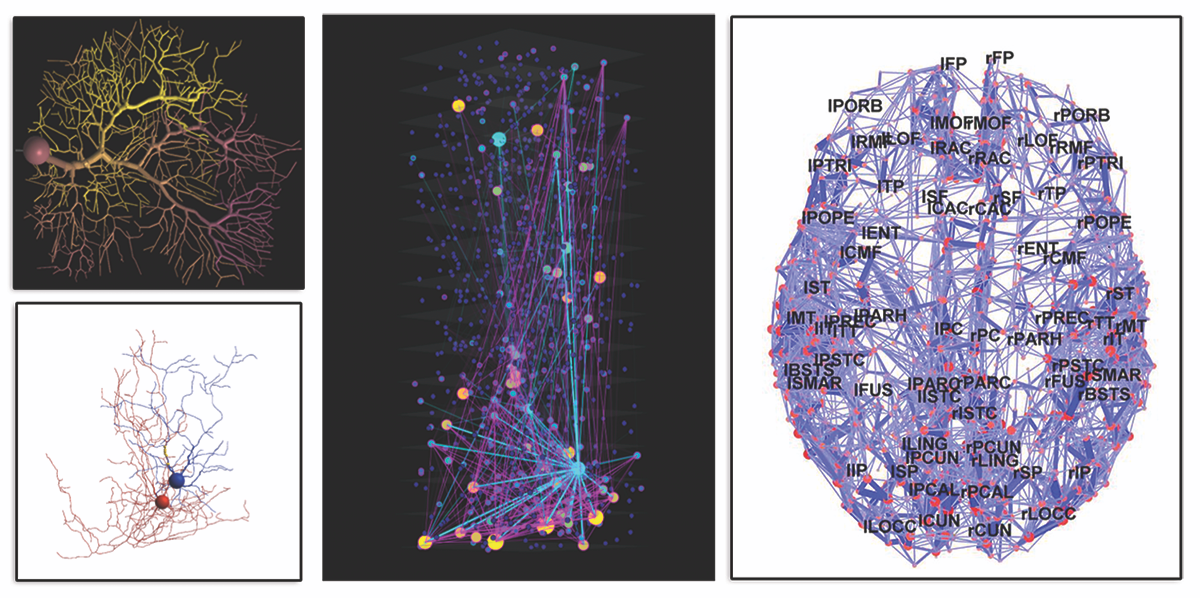
\includegraphics[width=0.8\textwidth]{./images/3typesmodels.png}
\caption[Layout by Pamela Payne. Top Left: ; Bottom Left: ; Middle: Screenshot by Zach Tosi ; Right: From Hagmann et al., 2008 \cite{hagmann2008mapping}, Licensed Under CC BY]{Micro, meso, and macro-level models in computational neuroscience. Left: micro-level models of individual neurons. Middle: meso-level model of a network of several thousand neurons. Right: macro-level model of neuronal connections spread out through the entire brain.}
\label{compNeuro}
\end{figure}
% http://medicalxpress.com/news/2013-11-entire-brain-brainbow-ii-technology.html
% https://upload.wikimedia.org/wikipedia/commons/thumb/e/ef/Network_representation_of_brain_connectivity.JPG/1280px-Network_representation_of_brain_connectivity.JPG

\emph{Micro-scale} models in computational neuroscience study individual neurons or even individual parts of neurons, like the receptors that are studded in the cell membrane to let charged particles in and out of a cell (these are models of ``receptor kinetics''). Models at this level often study the details of how charge flows through the tree-like structures of a neuron's dendrites and axons, and can accurately describe the behavior of individual neurons in a laboratory dish (``in vitro'') when they are injected with current from small electrodes. Models at this level often attempt to answer questions that are physiological or pharmacological in nature like the effect of neuromodulators on the low level dynamics of a neuron, or how new receptors are created or new dendritic spines are grown. These models are largely below the level of what is visible in a single Simbrain node.

\emph{Macro-scale} models in computational neuroscience describe the behavior of large groups of thousands to millions of neurons  and the connections between them. Oftentimes these models approximate the activity of thousands of neurons or even whole brain areas as the activity of a single higher level node.\footnote{As an example, see \url{https://www.ncbi.nlm.nih.gov/pubmed/21511044} \cite{cabral2011role}} These models can accurately describe the spatio-temporal organization of patterns of neural activity measured using brain imaging techniques like fMRI. In a Simbrain network simulation of this kind each node would represent the aggregate activity of thousands to millions of neurons and the whole network could represent the behavior of the entire brain. Models of this type are usually concerned with questions which are psychological or behavioral in nature. For instance the functional relationships between brain regions have been shown to be different in patients with schizophrenia resulting in a different overall graph structure of the functional connectivity between brain regions \cite{bullmore2009complex}. Often work at this level ``bleeds over'' into the realm of general neuroscience.

In this book we mostly focus on the \emph{meso-scale} (or ``middle''-scale) of computational neuroscience, between the micro and macro-levels. Whereas micro-scale models focus on individual neurons or their parts, meso-scale models focus on networks of \emph{hundreds to thousands} (or more) of interconnected neurons. And whereas each node in a macro-level model \emph{approximates} the activity of large group of real neurons, each of the simulated neurons in a meso-level simulation  corresponds to a real neuron. Thus, a meso-level simulation containing 1000 artificial neurons is a direct simulation of a biological neural network containing 1000 real neurons. The emphasis is on discerning governing principles and dynamical phenomena associated with these networks. Meso-level models in computational neuroscience have been implemented in Simbrain (e.g. the middle image in Fig. \ref{compNeuro}). 

The model neurons and synapses used in these simulations  are  more complex than the simple nodes and weights described above in Sect. \ref{structureNets},  since they are designed to mimic the electrochemical properties of real nerve cells. Most neuron models in computational neuroscience are governed by equations acting on variables which represent specific electrochemical attributes of living neurons. Synapses have temporal delays and their signals have duration. Network models in computational neuroscience tend to be comprised of \emph{spiking neurons} (neuron models which produce and propagate signals via action potentials) embedded in complex \emph{recurrent} networks. We cover the special properties of these model neurons and networks in chapter \extref{ch_spiking}.\footnote{In contrast to the micro-scale, which is (broadly) concerned with physiology, and the macro scale, which is often concerned with psychology, the meso-scale concerns itself with questions like: How do networks of interconnected neurons represent information? Can we replicate synaptic connectivity using plasticity rules? How does information processing emerge from the interactions of neurons embedded in a neural network?'  Meso-scale models often attempt to understand formalisms that describe observations of groups of neurons (e.g. slices of brain tissue) with explanations of those observations using models of detailed low level processes at the micro-scale. It is known that when neurons fire in particular temporal sequences the synapses connecting them will become stronger or weaker depending upon that sequence. A micro-scale model might concern itself with how new receptors are created, or new spines are grown. A meso-scale model will only concern itself with the function translating that temporal sequence into a change in synaptic strength.} 

Very roughly, the focus of computational neuroscience at these  three scales can be thought of as follows:
Neuron Dynamics $\rightarrow$ Network Dynamics $\rightarrow$ Brain Dynamics

\section{Connectionism}\label{connectionism}

% Need a footnote or paragraph just surveying a lot of the work in this area.  Also put in another link to this table with papers involving lesions and ablation studies of neural networks: \url{https://link.springer.com/article/10.1007/s42113-020-00081-z/tables/1}

% I think Smolensky's PTC is the best overall discussion.  While the level of analysis adopted by most connectionist cognitive models is not the conceptual [symbolic] one, it is also not the neural level." See the discussion surrounding 7.  Then can refer back to this in history and in intro symbolic vs. parallel. Nice distinction between activation evolution equation and connection evolution equation.

% See Talking Nets 259, 283, 274
% Maybe talk more about semantic memory and semantic network models, and contrast with other types of memory (many will not have taken intro cog-sci courses)
The use of neural networks as cognitive models, which behave in the same way humans and animals do, but without concern for neural realism, is sometimes called \glossary{connectionism}.\footnote{Not everyone using the term ``connectionism'' in this way, but it is a fairly standard usage. A more precise phrase would be ``connectionist model of a cognitive process''.}  In connectionist models, there is no direct effort to understand the brain. The focus is on modeling some aspect of human or animal behavior using nodes and weights. Such models  are usually meant to {\em suggest} how a given task is accomplished by the brain---they are ``neurally plausible''---but they do not directly model the underlying neuroscience.

% Should this be a named section on IAC? Kind of lost in this organization.
% Redo IAC given assignments
% Forward reference to ch_unsupervised_recurrent and DST, it develops fixed point attractors and the transient portion is the thought process
% We have settled on object pool and property pool. Introduce this nomenclature and distinguish it from the original.  Also, use some memory language. Item vs. category retrieval. "exemplars. It can also generalize along an indefinite number of different lines retrieve the specific characteristics of particular exemplars , and fill in plauaible default values for misaing properties."
As an example, consider the ``IAC'' or ``Interactive Activation and Competition'' network. A famous example of an IAC network is McClelland's model of knowledge of two fictional 1950s gangs, the Jets and Sharks from {\em West Side Story} \cite{mcclelland1981retrieving}.\footnote{For a video overview of this network in Simbrain, see \url{https://www.youtube.com/watch?v=Nw3TEDfugLs}.}

\begin{figure}[h]
\centering
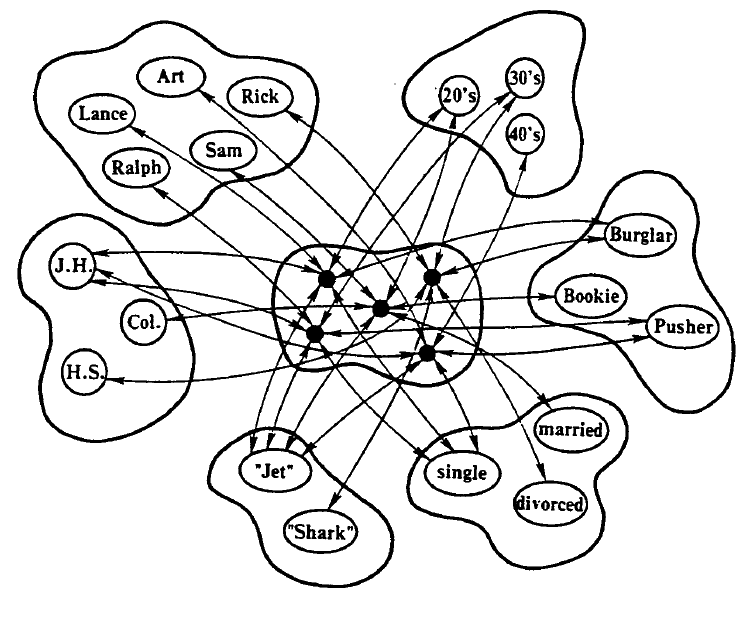
\includegraphics[scale=.3]{./images/IAC_JetsSharks.png}
\caption[From McClelland and Rumelhart, 1989 \cite{mcclelland1989explorations}.]{A fragment of the Jets and Sharks model. Nodes in this model don't represent neural activity, but activation of concepts in semantic memory.}
\label{iac}
\end{figure}

% Maybe just go full Simbrain. Change the example and make clear that it can be done in many ways.

% In a sense a model of the ventral stream, but not the dorsal stream. No ``embodied'' memory captured, no dorsal stream, and no retrieval mechanisms. Maybe refer to publications about actual semantic memory. BUT don't want to emphasize neuro too much so a balance.
% A good contrast to supervised, unsupervised, and generalization. A strange case where we hand-tune the weights. Note there is NO learning in these model. So the concepts of supervised and unsupervised don't apply. It is hand tuned. 

% Make the object pool / property pool distinction more central, and give more examples. There is no rock solid way to define object vs property philosophically, but functionally there are things we're talking about, and then there are our beliefs about their properties and characteristics.  The objects is like a thing that is a locus of these believes so they are in the center.  In IAC it's the people but it could also be teams, games, etc. (philosophers would wince, because object pools can even be properties)! Whatever is central is the object nodes,  // Also note that we stopped making separate name and object nodes. Maybe we could just call them name nodes.

An IAC model is organized into pools of nodes. In Fig. \ref{iac}, there are 7 pools of nodes. These pools of nodes are used to model the internal concepts of a person who knows about these two gangs. The pools represent different  traits:  age, education level, marital status,  job, etc. The central pool is a pool of ``instance nodes'' or ``object nodes'', shown as black disks, which correspond to individual people. Each person is associated with a node. The other pools correspond to properties of these people: their name, job, age, and gang affiliation. The nodes in each pool inhibit each other, which produces a \emph{winner-take-all} structure. As the simulation runs, the activation of one node in each pool will tend to dominate the others. Notice that the topology of this network is recurrent, and as a result the network has dynamics: when we run it, activation starts to spread from one node to another over time. In fact, these have also been called \emph{spreading activation} networks \cite{mcclelland1981retrieving}. 

The IAC network models general features of human semantic memory, like the ability to retrieve attributes of a person based on their name. If the Lance node is activated and the simulation is run, activation will spread through the recurrent network, and after a while the Jets node, 20s node, Junior high education node, and burglar node will have the highest activations. This is like asking ``Tell me about Lance?'' and being told about him. The network can also model our ability to describe the properties of a group of people. If the Jets node is activated and the network is run, the standard characteristics of the Jets will light up: they tend to be in their 20s, with a junior high school education, and single. This is like asking ``Tell me about the Jets?'' and being told about that group. The network can also model our ability to identify people who match a specific description. If the 20s node and the junior-high education node are activated, then the name nodes for Lance, Jim, John, and George all light up. This is like asking ``Who is in their 20s with a junior high education?'' and being told ``Well, that could be Lance, Jim, John, or George.''
%\footnote{Notice that the nodes and connections in this model don't correspond to actual neurons or synapses. The IAC network captures the empiricist theory (associated with John Locke and David Hume) that  human knowledge is encoded in abstract associations between ideas. Node activations correspond to the presence of an item in thought or memory, or what the empiricist philosophers called \emph{ideas}. If the ``Lance'' node is active, that corresponds to a person thinking about Lance. Connections between nodes correspond to \emph{associations} between ideas. The whole network of connections represents our overall knowledge about something, in this case, two gangs. When one node  is activated and the network is run, all the associated nodes are activated. Over time all the ideas associated with the original idea should be activated \cite{mcclelland1981retrieving}. Nodes and weights represent ideas and associations in an abstract brain-like way without modeling neuroscience directly.} \cite{mcclelland1981retrieving}

Though IAC networks are models of semantic memory, and are brain-like (spreading activation and winner-take-all types of dynamics do occur in the brain), they are \emph{not} models of the brain, they do not capture any details of human neuroscience, or have nodes whose activation corresponds to activity in specific parts of the brain.

\begin{figure}[h]
\centering
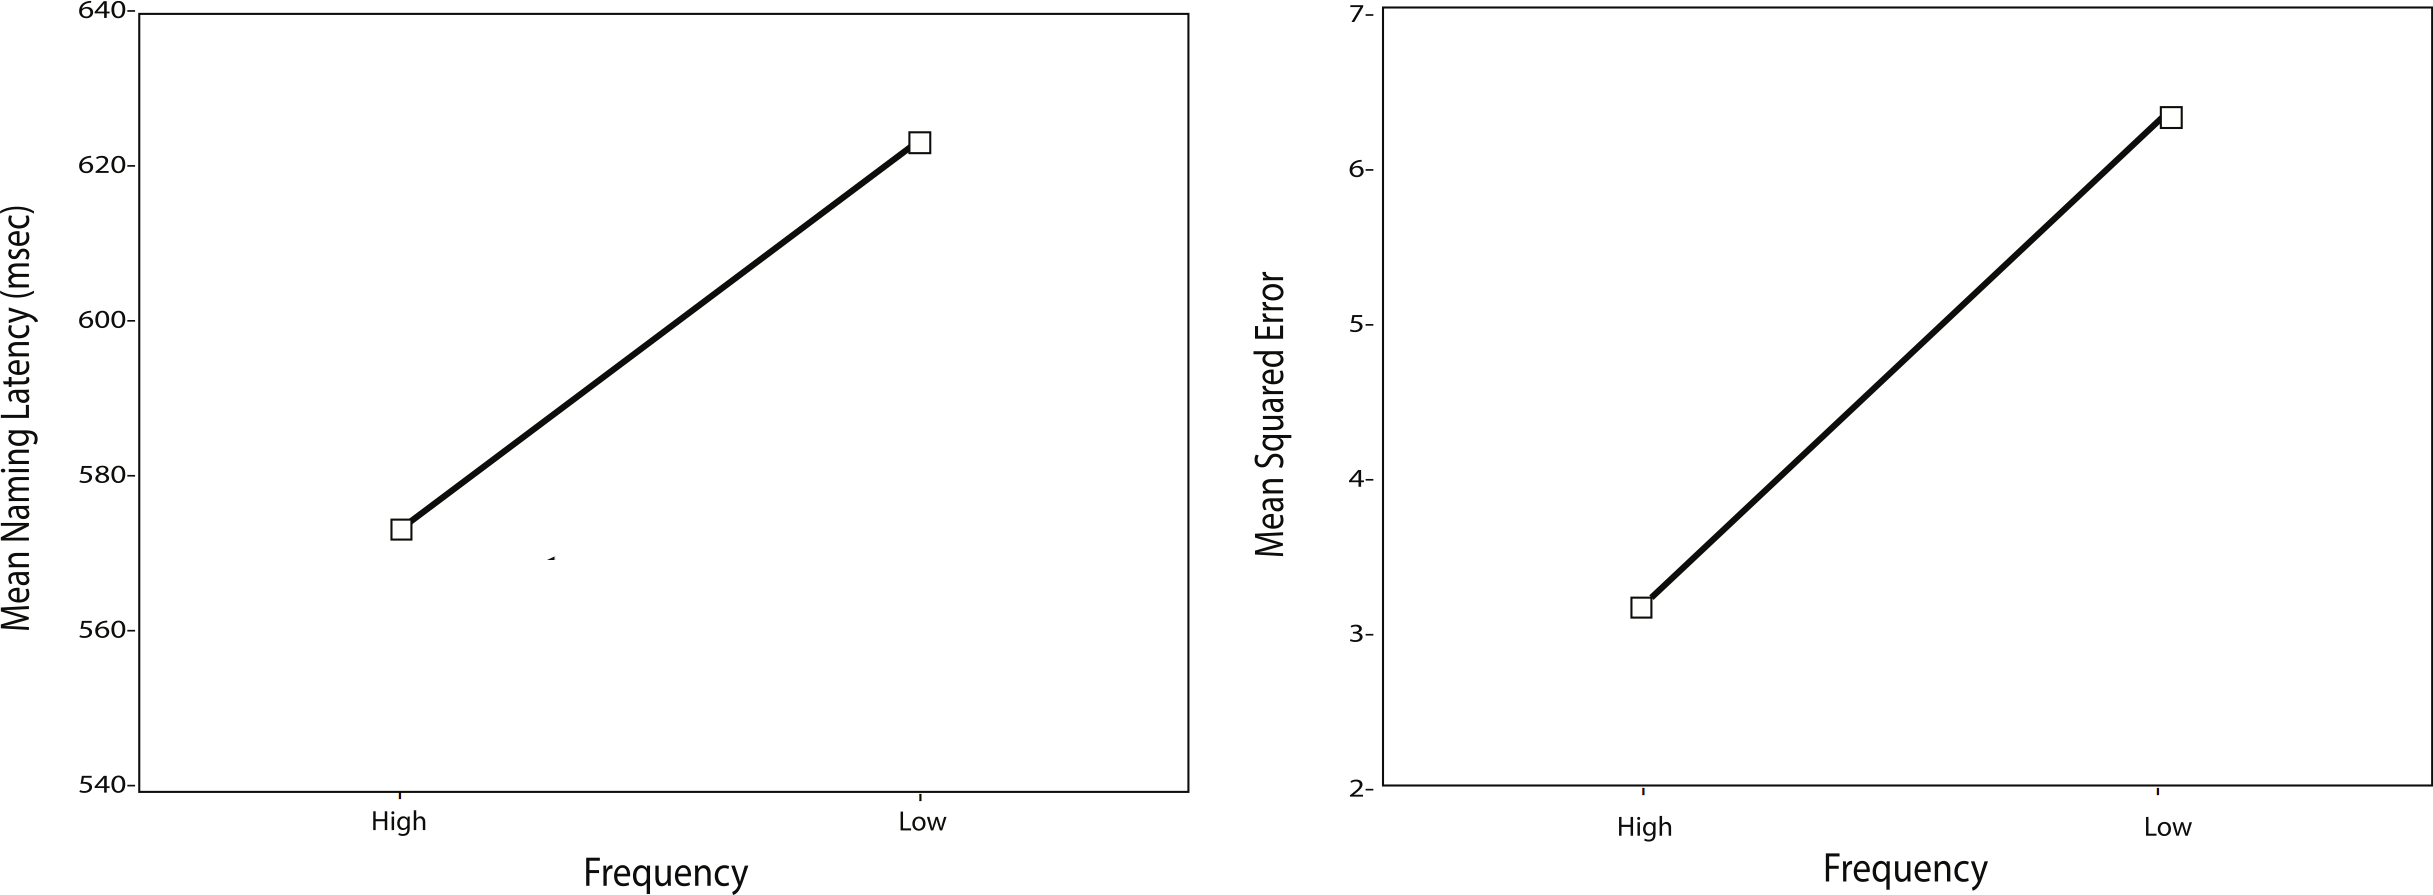
\includegraphics[width=0.8\textwidth]{./images/seidWordNet_Data3.png}
\caption[From McClelland and Seidenberg, 1989 \cite{seidenberg1989distributed}. Redrawn by Pamela Payne.]{Data associated with Seidenberg and McClelland (1989)'s reading model. Human data are on the left, neural network data are on the right. Humans pronounce high frequency words more quickly than low-frequency words. The neural network makes fewer errors on high frequency than low-frequency words.}
\label{regularityData}
\end{figure}
 
% This has become so short it might be time to get remove it, keep things simple. One main example per section. As it is it gets a bit lost. If used, take the opportunity to talk about error in a bit more detail.
The IAC network is a qualitative model of human memory. Other connectionist simulations are more quantitative. For example, Seidenberg and McClelland modeled childrens' reaction times in reading words aloud. The network is a variant on a feed-forward network, similar to the network on the left side of figure \ref{nn_types}. It has  more nodes: 400 input units, which represent written words, and 460 output units, which represent spoken words. It was trained to pronounce all one-syllable words in English using a method called ``backpropogation'' (chapter \extref{ch_supervised}). This simulation models  the \emph{word frequency effect}. Words that occur frequently in language (like ``the'') are pronounced more quickly than words that occur infrequently (like ``rake'').
%\footnote{\label{exceptionsVsRegular}The model also captures the ``frequency-regularity interaction'', whereby words that have regular pronunciation patterns (e.g. ``gave'' or ``must''), are pronounced faster than exception words (e.g. ``have''  or ``pint''). However, this regularity effect only occurs for infrequent words. This is also shown in the figure: in each graph the upper curve with the open squares show exception words; the lower curves with filled triangles show regular words.}  

Human data showing this effect are on the left side of Fig. \ref{regularityData}. Humans pronounce high frequency words more quickly than  low frequency words (the $y$-axis shows latency, or length of time to pronounce the word; lower values mean faster times). The neural network data on the right  was generated by counting how many mistakes the network made for low and high frequency words \cite{seidenberg1989distributed}. When you line the two graphs up next to each other, they look the same. This suggests that the way the model reads is similar to the way humans read: both the neural network model and humans are better at reading more common words.
%\footnote{ Many questions come up here, and you might not be satisfied (in fact, this model was involved in a kind of war between connectionist and non-connectionist models of  reading). The main thing  to emphasize here is that the model is supposed to capture some kind of human, behavioral data.}

\section{Computational Cognitive Neuroscience}\label{mixedCases}

 For neural network used as scientific models, it can be hard to say whether it simulates the brain (computational neuroscience), or cognition (connectionism). Many models aim to do both at once.
That is, many people who use neural network models are interested in \emph{both} how the brain works \emph{and} how cognition works, and of course, how the two are related. Thus, there are increasingly many models that attempt to capture both neural and psychological data, as was noted in the discussion of macro-level computational neuroscience above. 

We will refer to these as \glossary{computational cognitive neuroscience} models, and define them as models that attempt to capture psychological and behavioral data while simultaneously paying attention to neural details. This type of model captures various aspects of cognition (e.g. visual attention, semantic and episodic memory, priming, familiarity, and cognitive control), using groups of neurons that are explicitly associated with specific brain circuits. Many researchers hope that over time computer models of brain and behavior will converge, and that future models will increasingly capture both neural and behavioral data, and thereby reveal how the dynamics of the brain give rise to the dynamics of cognition.\footnote{Examples of researchers and research groups working in this area include the work of Randy O'Reilly and his colleagues (\url{https://grey.colorado.edu/CompCogNeuro/index.php/CCNBook/Main}), Stephen Grossberg's work which began in the 1960s (\url{https://en.wikipedia.org/wiki/Stephen_Grossberg}), and the work of Chris Eliasmith and his colleagues (\url{https://uwaterloo.ca/centre-for-theoretical-neuroscience/people-profiles/chris-eliasmith}). There is also a burgeoning research community organized around the computational cognitive neuroscience conference (here is their 2024 program: \url{https://2024.ccneuro.org/}).} Some examples of this type of model are shown in figure \ref{ccn}.

% Emergent ref since I have a spaun ref?
\begin{figure}[h]
\centering
\raisebox{-0.5\height}{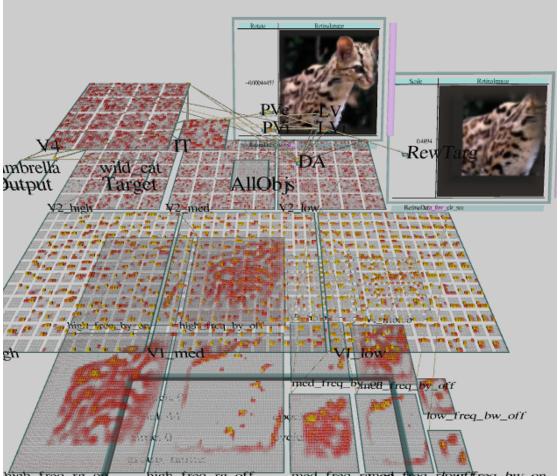
\includegraphics[scale=.3]{./images/EmergentScreenshot.png}}
\hspace*{.4in}
\raisebox{-0.5\height}{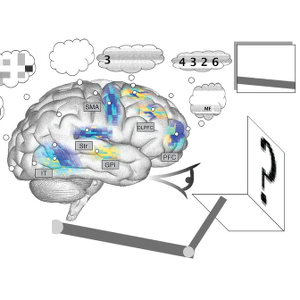
\includegraphics[scale=.6]{./images/spaun.png}}
\caption[Left: From \url{https://grey.colorado.edu/emergent/index.php/File:Screenshot_vision.png}; Right: Spaun screenshot. Cf. \cite{eliasmith2012large}.]{(Left) An Emergent simulation of visual processing, with labels indicating which brain areas each group of nodes represents. (Right) A Nengo simulation of the human ability to retrace a visually perceived number.}
\label{ccn}
\end{figure}

 From this standpoint, computational neuroscience and connectionism are two ends of a continuum or spectrum. We have computational neuroscience at one end, and connectionism at the other. All through the middle of this spectrum are models that try to model both biological data and psychological data at the same time. The goal is to understand how the circuits of the brain produce all the wealth and complexity of observable human and animal behavior. 

\section{From science to engineering and from engineering to science}

Some neural networks that originated as scientific models later informed the development of engineering tools. Conversely, sometimes an engineering tool ends up being useful as a scientific model. These are interesting historical dynamics. A prominent example are LLMs like ChatGPT. They originated as pure engineering, something useful. But now they have become an intense topic of scientific interest as linguists, cognitive scientists, philosophers and others ask to what extent they can tell us about human cognition (see section \extref{llm_analsis}).
 
 Deep networks provide a good example of these back and forths. Deep neural networks  were originally used as scientific models of vision in the 1970s (see chapters \extref{ch_history} and  \extref{ch_neuro}).  These early neural network models of vision turned out to be excellent tools for pattern recognition, a common engineering application, for example recognizing digits on an envelope. This is part of what led to the deep learning revolution of the 2010s. So we had a shift from science to engineering. But then it happened again, in the reverse direction. These new and improved deep networks turned out to be useful in computational neuroscience as a way to understand the human visual system. So, a neural network that started off in science, then got used for engineering, and then later that tool got adapted back to science! 

Similar twists and turns from engineering to science are happening now with the emergence of large language models like ChatGPT. They originated as pure engineering models, that are meant to facilitate natural language processing. I think we can all agree that ChatGPT is useful, whether or not it ``thinks like a human.'' But it's so compelling as a model, that linguists, psychologists, and philosophers are starting to study them as cognitive models.  See Chapter \extref{ch_supervised_recurrent}. So in this case a model that started off in engineering subsequently became an object of scientific study.

% Forward reference to the strange case of BERT
%\chapter{History of Neural Networks}\label{ch_history}
\chapterauthor{Jeff Yoshimi, Pierre Beckmann}{.95, .05}

% Consider separating second winter, and deep learning resurgence, even if the resulting sections are short, for a cleaner presentation.
% Can say more about the two resurgences.  Both involves more on learning intermediate reps in FF networks. Part of a narrative across chapters
% Add AI Winter and Lighthill as contemporaneous
% Add more explicit discussion of neobehaviorism and Clark Hull (search Hull below)

This chapter briefly outlines the history of neural networks, including the pre-history of neural networks and cognitive science extending back to ancient Egypt. The theory of neural networks has many historical precedents, but emerged as an explicit mathematical and computational formalism in the mid 1900s, via the work of McCulloch and Pitts. The main events developed in the chapter are shown in Fig. \ref{timelineHistory}. 

\begin{figure}[h]
\centering
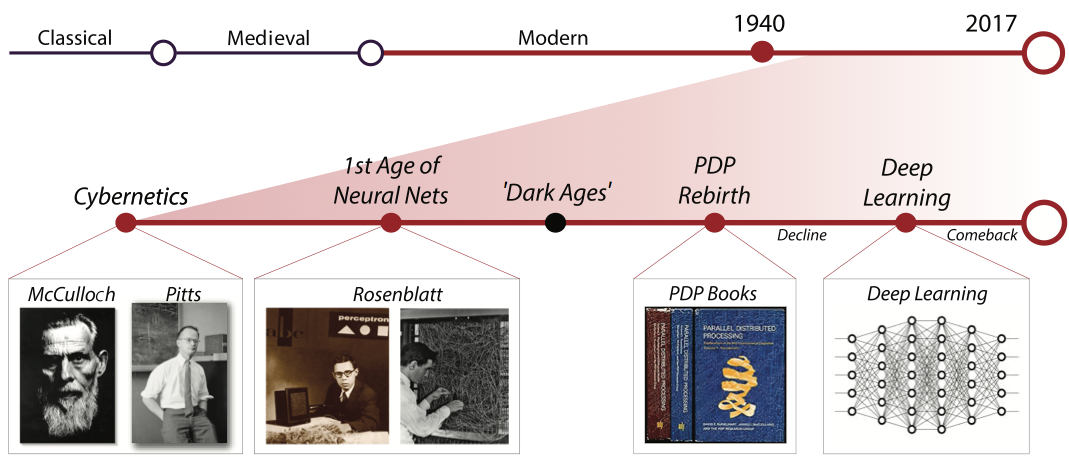
\includegraphics[width=0.8\textwidth]{images/historyTimeline.png}
\caption[Pamela Payne and Jeff Yoshimi.]{A timeline of the history of neural networks. The main history of neural networks runs from the mid 1940s to the present. We  also consider some of the pre-history of neural networks,  i.e. historical figures who linked the structure and dynamics of the mind with the structure and dynamics of the brain.}
\label{timelineHistory}
\end{figure}
% Black dot for second decline to match first

\section{Pre-history}

Cognitive science, the interdisciplinary study of mind, has ancient roots. Documentation of the idea that the brain plays some role in controlling behavior goes back to an Egyptian papyrus that is over 3000 years old.\footnote{The papyrus can be viewed online; try searching for ``Smith papyrus''. Recent scholarship on the papyrus is collected in \cite{meltzer2014edwin}.} Hieroglyphics from the papyrus describing the gyrations of the brain are shown in Fig. \ref{papyrus}. 
% Source: https://www.princeton.edu/~cggross/Hist_Neurosci_Ency_neurosci.pdf

\begin{figure}[h]
\centering
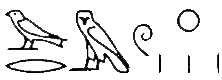
\includegraphics[width=0.4\textwidth]{images/papyrus.png}
\caption[From \url{https://faculty.washington.edu/chudler/papy.html}]{Hieroglyphics describing the sulci and gyri of the brain.}
\label{papyrus}
\end{figure}

In Western philosophy and science, Plato, Aristotle, and other Greek philosophers had an interest in the structure of the human mind (or ``soul'') in relation to physical processes in the body.\footnote{I focus on Western roots of neural network theory, though there were precedents in other parts of the world, which I hope to add in future versions of this chapter. Currently, the literature is sparse. There is an expanding literature on the history of science globally (e.g \cite{selin2013encyclopaedia}), but there is not (as of 2017) much scholarship on the history of neuroscience, cognitive science, or psychology in Africa, Asia, India, Mesoamerica, the Middle East, and other regions whose historical documents contain relevant information. There is however, some literature on  Arabic and Islamic roots of neuroscience \cite{mohamed2008arab}.}  Plato and Aristotle both described the soul as a set of interacting faculties (in Plato: reason, spirit, and appetite), and both speculated about its physical basis. They disagreed  about whether the brain or heart is the physical basis of the soul (Aristotle thought the brain just cooled the blood), but by the end of the Classical period the dispute was resolved in favor of the brain \cite{finger2001origins}.

In the Medieval period, priests, physicians, and natural philosophers throughout Europe and the Middle East discussed cognition in relation to the brain. Cognition was thought to be based on the play of ``spirits'' or vapors in the ventricles of the brain \cite{finger2001origins}. Spirits originating in the senses were combined in the ``common sense'' and then purified, and mixed in higher ventricles. A typical diagram from the period is shown in figure \ref{medieval}. The ventricles are now believed to be shock-absorbers and chemical reservoirs. They are not thought to play a central functional role in cognition. However, the idea that sensory inputs to the brain are combined and refined in various ways persists in connectionist models.
% https://web.stanford.edu/class/history13/earlysciencelab/body/brainpages/brain.html   // Mention Avicenna here
% One of the animal internal faculties of perception is the faculty of fantasy, i.e., sensus communis, located in the forepart of the front ventricle of the brain. It receives all the forms which are imprinted on the five [external] senses and transmitted to it from them. Next is the faculty of representation located at the rear part of the front ventricle of the brain, which preserves what the sensus communis has received from the five senses even in the absence of the sensed object. … Next is the faculty of the 'sensitive imagination' in relation to the animal soul, and the 'rational imagination' in relation to the human soul. This faculty is located in the middle ventricle of the brain near the vermiform process, and its function is to combine certain things with others in the faculty of representation, and to separate some things from others as it chooses. Then there is the estimative faculty located in the far end of the middle ventricle of the brain, which perceives the non-sensible intentions that exist in the individual sensible objects, like the faculty that judges that the wolf is to be avoided and the child is to be loved. Next there is the retentive and recollective faculty located in the rear ventricle of the brain, which retains what the estimative faculty perceives of the non-sensible intentions existing in individual sensible objects. (Avicenna, translated in Rahman 1952, p. 31)
% https://www.acsu.buffalo.edu/~duchan/new_history/middle_ages/ventricular_theory.html


\begin{figure}[h]
\centering
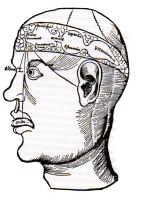
\includegraphics[width=0.2\textwidth]{./images/humoral.png}
\caption[From Gr\"{u}sser, 1990 \cite{grusser1990seat}]{A medieval diagram which shows how spirits were thought to flow and combine through the ventricles of the brain. Different ventricles were associated with different faculties, such as sensation and the ``common sense,'' integrating different senses, imagination, memory, and reason.}
\label{medieval}
\end{figure}

%Descartes?
During the Enlightenment, many speculated that connections between ideas in the mind are based on connections between fibers in the brain (neurons had not yet been identified as distinct structures.)\footnote{For more on this period of history, see Sutton (1998) \cite{sutton1998philosophy}. Sutton's discussion of Descartes is especially interesting, since it shows how Descartes had a connectionist styled account of the brain, which on his view  interacts with a non-physical soul via patterns of activity at the pineal gland. Other mechanist philosophers of the period such as Hobbes and La Mettrie had similar accounts but rejected the assumption of a non-physical soul.} In the 1700s, the empiricists Locke, Berkeley, and Hume famously claimed that ideas in the mind result from associations between simple sensory ideas: for example, a percept of an apple is composed out simple sensations corresponding to its color, shape, smell, and taste. One idea comes to mind, it calls another to mind, etc. Sometimes this happens instantaneously, as in the apple percept, but in other cases it might unfold in a temporal progression. Someone mentions apples, and that might make you think of fiber, which might in turn make you think of Raisin Bran. If someone mentions a person you know, associated thoughts about them--their age, where they live, their occupation, physical appearance, etc.--might also come to mind. One idea comes to mind, it calls another to mind, etc. Thus, the empiricists thought of the mind as something like an Interactive Activation and Competition (IAC) network (cf. Chapter \extref{ch_intro}) \cite{bain1873mind}.

In this period, David Hartley argued that the empiricist theory of associations could be explained by laws governing connected neurons \cite{hartley1834observations, bain1873mind}. For example, Hartley \cite{hartley1749observations} proposed that sensations $A,B,C,...$ which are associated with each other, are associated because of correlated associations between ``vibrations'' of brain fibers:
\begin{quotation}
PROPOSITION 10: Any sensations $A, B, C$, etc., by being associated with one another a sufficient number of times get such a  power over the corresponding ideas $a, b, c$ etc., that any one of the sensations $A$, when impressed alone, shall be able to excite in the mind $b, c,$ etc., the ideas of the rest.

PROPOSITION 11: Any vibrations $A, B, C,$ etc., by being associated with one another a sufficient number of times get such a  power over the corresponding miniature vibrations $a, b, c$ etc., that any one of the vibrations $A$, when excited alone, shall be able to excite in the mind $b, c$, etc. 
\end{quotation}
He proposed proposition 11 as a neural explanation of proposition 10, which is psychological. Note that proposition 11 is an early version of what would later became known as Hebb's rule or Hebbian learning (``neurons that fire together, wire together''), discussed below and in chapter \extref{ch_unsupervised}.

Later, in the 19th century, Bain illustrated these ideas with images that look strikingly like modern neural network diagrams, as in Fig. \ref{bain}.

\begin{figure}[h]
\centering
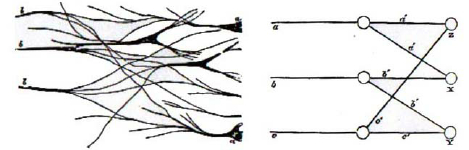
\includegraphics[scale=.7]{./images/bain.jpg}
\caption[From  \cite{bain1873mind}, pp. 110-111.]{From Bain's 1873 book \emph{Mind and Body}, which opens with the question ``What has Mind to do with brain substance, white and grey''?}
\label{bain}
\end{figure}

The notion that associations between thoughts and memories are based on neural connections in the brain was further developed in late 1800s by Sigmund Freud, who developed a psychodynamic theory, according to which  psychical ``energies'' are based on the flow of activations in the neural networks of the brain. His goal was to show how psychology could become a natural science by representing ``psychical processes as quantitatively determined states of specifiable material particles'' \cite[p. 355]{freud1954project}. But whereas earlier theorists had simply speculated about associative processes, he based his on actual  clinical observations, and in particular observations of (allegedly) neurotic patients experiencing ``excessively intense ideas.''  He explained his clinical observations in terms of ``neuronic excitation'' understood as ``quantities in a condition of flow'' (p. 356). Fig. \ref{freud} shows part of an image from this early book, which describes a patient (Emma Eckstein, who went on to become a famous author) who avoided shops based on an earlier traumatic experience. The specifics of the account are dubious, and Freud himself gave up on the project of a direct neural account of psychological processes,  but it does show that Freud was thinking about the mind in a broadly connectionist way.

\begin{figure}[h]
\centering
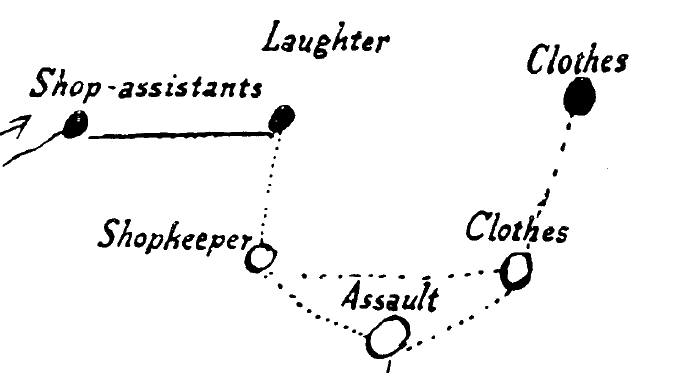
\includegraphics[width=0.5\textwidth]{images/freud_scientific_psychology.png}
\caption[From \cite{freud1954project}.]{An image from Freud's early \emph{Project for a Scientific Psychology}. The open circles are conscious ideas; the dark circles are unconscious ideas. }
\label{freud}
\end{figure}

% More on neuron doctrine, and how recent work may provide some limited support to Golgi? https://www.science.org/doi/10.1126/science.ade5645
Many other psychologists, neuroscientists, and philosophers in the late 19th and early 20th century contributed to the general idea that psychological processes are rooted in neural processes. Helmholtz, Mach, Ram{\'o}n y Cajal, Golgi, and others advanced biological psychology in various ways (see, e.g., \cite{boring1929history}), e.g. by establishing that neurons are individual cells, and by applying mathematical methods to psychology and neuroscience. In Russia, the psychologists Luria and Pavlov sought to understand the neural basis of associative learning, speech pathology, and other cognitive phenomena in a quantitative, experimentally tractable way.\footnote{On Luria in relation to the history of neural networks, see \cite[p. 41]{rumelhart1986parallel}.}

\section{Birth of Neural Networks}

We now turn to the history of neural networks proper, i.e. explicit formal descriptions of artificial neural networks, which could be implemented in computer programs.\footnote{The history of neural network research from this point forward is covered in several places. Fausett has a 4 page overview that covers the main points nicely: \cite[pp. 22-26]{fausett1994fundamentals}. Levine, ch. 2 is especially detailed on McCulloch,s Pitts and Rosenblatt \cite{levine2000introduction}. A brief online history is at \url{http://cs.stanford.edu/people/eroberts/courses/soco/projects/neural-networks/History/}. A more recent history that extends to present day work in deep learning is at \url{https://www.skynettoday.com/overviews/neural-net-history}. A comprehensive discussion that is highly attentive to historical details often overlooked by others is Schmidhuber's ``Deep Learning: Our Miraculous Year 1990-1991'' \cite{schmidhuber2020deep} (don't let the title fool you, it considers earlier work). See \url{https://people.idsia.ch/~juergen/deep-learning-miraculous-year-1990-1991.html}.  Also see the end of chapter 1 of the first PDP chapter, \cite{rumelhart1986parallel}, and Haykin (2nd Ed.) section 1.9 \cite{haykin1998neural}. My favorite source is a series of interviews of leading figures in the history of neural networks collected in \emph{Talking Nets}, \cite{anderson2000talking}.} 

The first wave of research into neural networks occurred in the 1940s, via an array of neuroscientists, mathematicians, logicians, and engineers, many of them at MIT.\footnote{Important research relating to neural networks did occur earlier in the 20th century, e.g. work by Thorndike, Lashley, and Clark Hull. Hull's writings contain diagrams and formulas describing associative learning processes based on rat studies that look very much like connectionist networks (e.g. \url{http://psychclassics.yorku.ca/Hull/Hierarchy/part1.htm}).}   The history is complex, fascinating, and brimming with colorful personalities (see the early chapters of \cite{anderson2000talking}). This was the period when digital computers were first being developed by people like John von Neumann, a child prodigy who  later established a computer architecture still in use today (the ``von Neumann architecture'' \cite{von1981principles}). The architecture involves a separation between memory and a central processing unit that retrieves data from memory and operates on it using logical rules.
% Consider expanding the Hull discussion with a picture, esp. in light of the video

Neuroscience had also been steadily advancing in this period, and the network structure of the brain and its relation to behavior were better understood. The field of control theory was emerging via the work of Norbert Wiener, another child prodigy. He developed the field of ``cybernetics'' (which is closely related to modern control theory), and defined it as ``the science of control and communication in the animal and the machine'' \cite[p. 16]{wiener1948cybernetics}. In the late 1930s, the petroleum industry had developed central control systems to maintain refinery towers, and in WWII feedback systems were used to control anti-aircraft guns. A key idea in cybernetics was that these feedback circuits could coordinate complex movement, both in engineered systems and in the brain.

%  McCulloch: ``McCulloch was a psychiatrist and neuroanatomist by training: he spent some 20 years thinking about the representation of an event in the nervous system.
% Pitts. ```Pitt was a mathematical prodigy, who joined Mc Culloch in 1942.''
% They were logic oriented. Kleene had papers on this stuff. And these things emerged in the same literature as automata theory. Remember this is the beginning of formal logic and people realizing its potential.

In this atmosphere, two scientists emerged as the ``fathers of neural network theory'': Warren McCulloch (a neurophysiologist affiliated with cybernetics) and Walter Pitts (a logician).\footnote{Both had vivid personalities. McCulloch had wild hair and charisma. Pitts was a quiet introvert who had trouble getting a regular job, but who was regarded by his associates as a genius and was supported by McCulloch for many years. For a fascinating first-hand account of their personalities see the interviews with Lettvin, Cowan, and Arbib in \cite{anderson2000talking}. See in particular pages 9, 101, 104, 218, 223. Video interviews with McCulloch are available online.}  They wrote a famous paper  showing how neuron-like elements could perform all the logical operations performed by computers. This in turn implies that whatever can be done on a computer can, in principle, be done using neurons \cite{mcculloch1943logical}. A diagram from McCulloch and Pitt's famous paper, \emph{A Logical Calculus of Ideas Immanent in Nervous Activity}, is shown in figure \ref{mp}.\footnote{See Levine, p. 12, for a useful summary of how McCulloch / Pitts networks operate \cite{levine2000introduction}.}  In appendix \extref{ch_logicgates}, a demonstration of a similar approach to building logic gates using neural networks (in Simbrain) is developed.

\begin{figure}[h]
\centering
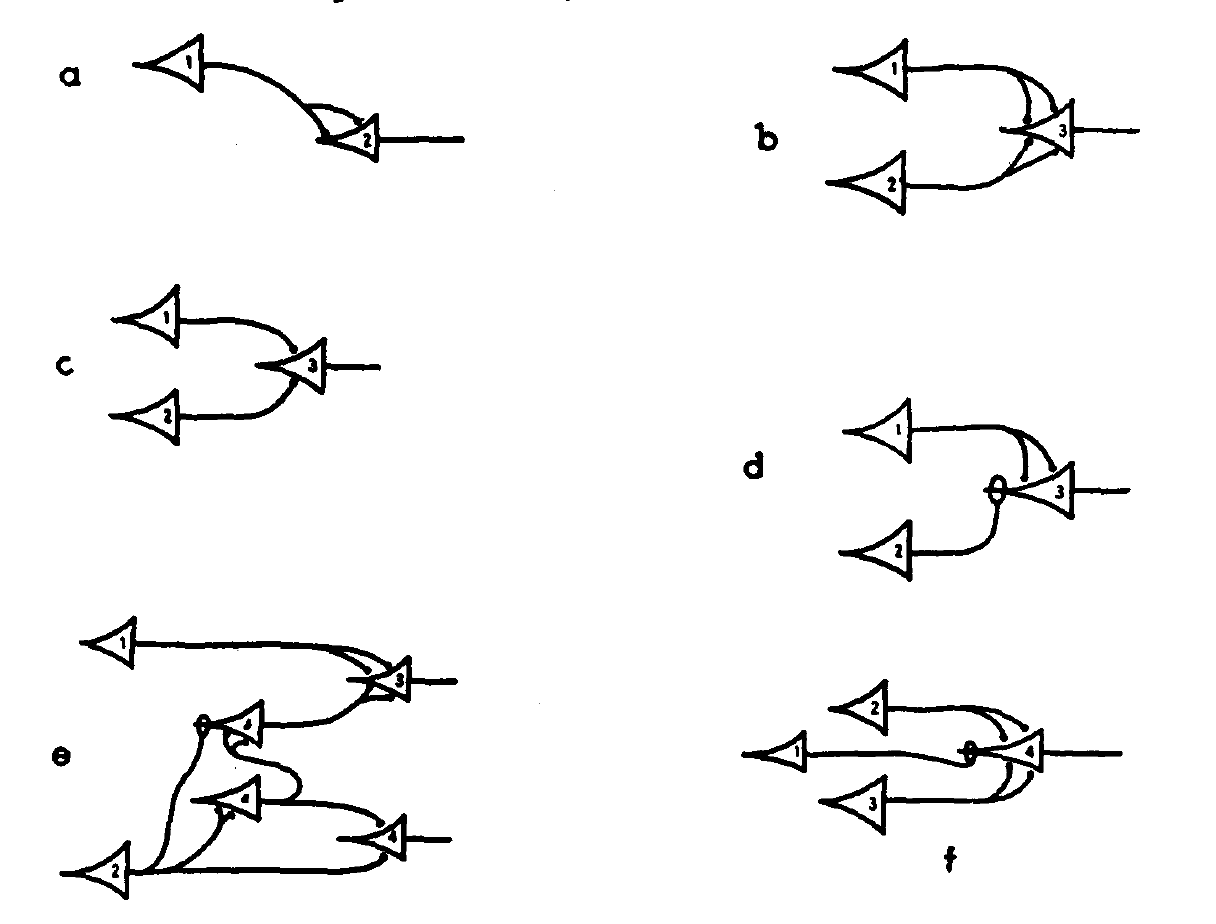
\includegraphics[width=0.5\textwidth]{./images/McCullochPitts.png}
\caption[From \cite{mcculloch1943logical}.]{From the end of McCulloch and Pitt's famous article, in which they demonstrate that ``for any logical expression satisfying certain conditions, one can find a net behaving in the fashion it describes.''  In these networks, what are today called ``weight strengths'' or ``synaptic efficacy'' correspond to number of connections. Nodes only fire if two or more incoming connections are activated. ``Lasso" connections correspond to what are today called ``inhibitory'' connections. In these networks, a single activated lasso connection will disable the node it is connected to. A network computing \emph{logical or} is shown in panel B (it will fire if either of the inputs nodes connected to it fires) and a network computing \emph{logical and} is shown in panel C (it only fires if both input nodes connected to it fire). Panel E models the heat illusion (briefly held cold objects can feel hot). For an elaboration of this case see \cite{piccinini2004first}.}
\label{mp}
\end{figure}
% Expand this. Explain the panel d is a connection with a shutoff, a bit like spiking 2 neurons and ch 1 ex.. Insert a reference to a Simbrain model of the heat illusion and include text from the video. // Maybe put labels in pic

McCulloch and Pitts used what are now called binary units or threshold units (see chapter \extref{ch_act_functions}): nodes that are only activated when their summed inputs are above a certain value. Nodes could only be active at a level of 0 or 1, based on the ``all or none'' property of neurons (cf. \extref{ch_neuro}). They made some assumptions that are unusual by today's standards. For example they assumed that a single inhibitory input is sufficient to completely prevent a neuron from firing. More importantly, they did \emph{not} describe connections between neurons using variable-strength weights. Their networks used fixed connections, which could not be adjusted using a learning rule. Learning rules would later become a  primary focus of neural network theorists. Nonetheless, it was the first time an actual formal model of a neuron was presented, together with a serious effort to understand how networks of neurons could produce complex behaviors.
% I think this is right, but check: \footnote{Though they did allow multiple connections between nodes, a multi-graph architecture not often used today.}

%Today neural networks are usually thought of in contrast to digital computers. In fact, in the introductory chapter \extref{ch_intro} we  opened by contrasting computation in a neural network with computation in a digital computer. But it is important to realize that this opposition came later. In this period people were just trying to figure out what a computer was. They were figuring out the mathematical underpinnings of computer science via the study of ``formal automata''. They knew the brain did some kind of computation and were interested in that. The neuroscientists were interested in what the logicians were doing. The engineers were interested in what the neuroscientists were doing. Etc. And in fact a neural network can implement a digital computer in principle. But in practice, the two styles of computation are distinct, and later on in the history the two approaches would be more strongly distinguished.

\section{The Cognitive Revolution}\label{cog_rev}

In the 1950s advances in linguistics, early computer science, neuroscience, and psychology, among others, coalesced in a broad reaction to earlier approaches to psychology, which had focused on observable behavioral data. The earlier \emph{behaviorists} had frowned upon discussions of internal processing between sensory inputs and motor outputs, and treated the mind as a kind of black box. The emerging cognitive scientists wanted to break open that black box and look inside: they wanted to understand what kind of processing occurs between sensory input and motor output in terms of \emph{computation}. The big idea that got everyone excited was that inside the mind there is an information processing system, one similar to the computer systems that were just then beginning to be realized on a large scale. This was sometimes referred to as the ``cognitive revolution'' in psychology.\footnote{An excellent overview and history of the era is \cite{baars1986cognitive}.}  

In the early cognitive revolution many different kinds of cognitive model were considered, including early neural networks like the Perceptron, discussed next. However, from early on there were doubts about neural networks. There were, for example, concerns that statistical approaches were fundamentally limited, a concern most famously posed by Minsky and Papert (see chapter \extref{ch_lms_backprop}). Others, were concerned that neural networks could not store and manipulate context-free symbols to use in reasoning \cite{fodor1988connectionism}, and there was also a worry that human-like language and reasoning could not be learned from the input stream used to train a neural network (``poverty of the stimulus'' arguments \cite{berwick2011poverty}). A competing approach to modeling cognition that avoided these problems was the symbolic approach---it goes by various names, including ``Symbolic AI'' and ``Classical AI''--according to which cognition involves manipulating symbols in accordance with rules (see section \extref{classicalAIComparison}). 

Over time, a kind of war broke out between these groups (brewing in the 1950s and peaking in the 1980s).  The connectionists had responded to the concerns raised by the symbolic AI camp, building networks that attempted to do all the things that symbolic AI advocates said they couldn't. The symbolic AI camp responded with doubts about these efforts, and for a time the ``framework wars'' were at the center of cognitive science. Today there are other camps as well, and some who mix ideas from both symbolic AI and connectionism. To jump ahead briefly, with the advent of large language models that produce convincing natural language, many feel that the Symbolic AI-connectionism war has been settled in connectionism's favor, and indeed  as noted in the introduction today ``AI'' is often used to refer to neural networks. But the symbolic approach has fought back against this, and in some sense the old debate has been rekindled (see section \extref{llmPhilosophy}).

Here are some themes in early cognitive science that prefigure connectionism. The Canadian psychologist and neuroscientist Donald Hebb formulated his famous learning rule for weights, the ``Hebb rule'' (``neurons that fire together, wire together'') \cite{hebb2005organization} (cf. the discussion of Hartley above).\footnote{See \url{http://www.scholarpedia.org/article/Donald_Olding_Hebb}. Also see Werbos' interview in  \cite{anderson2000talking}.}   Hebb also described the operation of the brain in terms of networks of connected neurons, formulating the concept of a ``cell assembly'', a group of neurons that becomes associated over time and thereafter tend to collectively reverberate in response to a stimulus (Fig. \ref{hebb} shows one of Hebb's own diagrams of a cell assembly) \cite{hebb2005organization}. The concept of a specific, learned pattern of brain activity produced by a stimulus remains important today.\footnote{See \url{http://www.scholarpedia.org/article/Cell_assemblies}. For a more up to date version of the idea cf. the concept of a polychronous neural group or PNG, \url{https://www.izhikevich.org/publications/spnet.htm}.}
% Need more information on the social network of Hebb. He does not seem too connected to the other figures.
% Some information in Haykin p. 38-39: ``Hebb's book was immensely influential among psychologists [like Anderson] but unfortunately it had little or no impact on the engineering community. Hebb's book [however] been the inspiration for the development of computational models of learning and adaptive systems" [Duda and Hart]   Uttley, leaky integrate and fire. 

\begin{figure}[h]
\centering
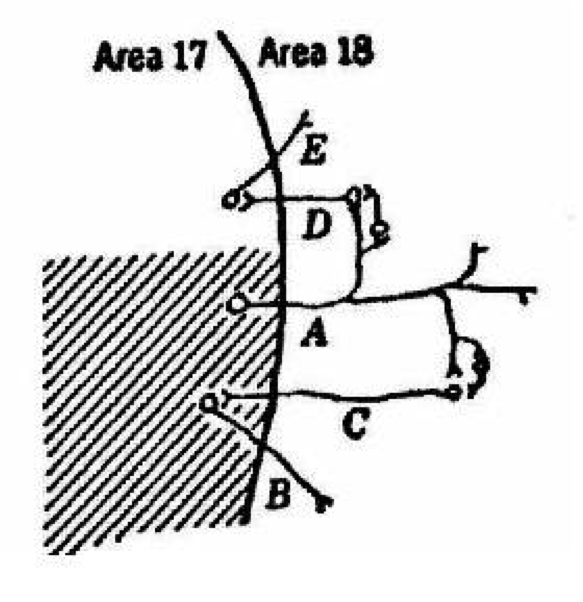
\includegraphics[width=0.4\textwidth]{./images/HebbCircuit.png}
\caption[From Hebb, 2005 \cite{hebb2005organization}]{A Hebbian cell assembly. These neurons initially fired together, and then got wired together, and so they will tend to fire together in the future.}
\label{hebb}
\end{figure}

\begin{figure}[h]
\centering
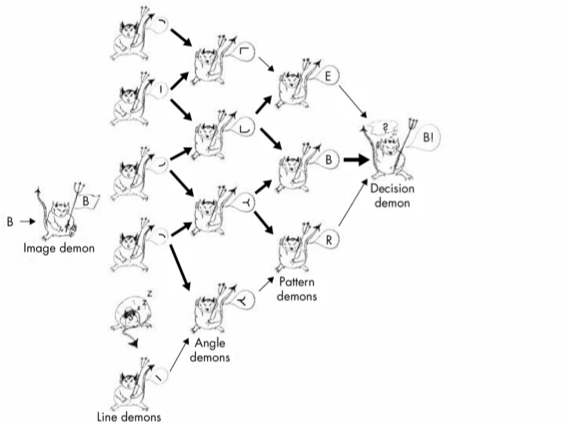
\includegraphics[width=0.5\textwidth]{./images/Selfridge.png}
\caption[From Groome, 2013 \cite{groome2013introduction}]{Selfridge's pandemonium model. Here the model is detecting the letter ``B''. The solid lines correspond to connections between active nodes, or ``demons''.}
\label{selfridge}
\end{figure}

Another important figure in the period was the psychologist Oliver Selfridge, who pioneered the idea that psychological processes can be broken down into interacting sub-processes. His ``Pandemonium'' theory described the mind as a collection of ``demons'', each of which takes care of one specific aspect of a task. For example, figure \ref{selfridge} shows how Selfridge thought of the process of perceiving the letter ``B''. As can be seen the figure, the demons are basically nodes and the model is basically a feed forward network. An image arrives at the eye, line demons detect lines and curves in various orientations, those demons send messages to the next layer of demons who detect combinations of lines and curves, etc. The process continues through a network of demons until a decision demon says ``B!'' \cite{selfridge1958pandemonium}.  This is a striking anticipation of the concept of a deep network for vision with layers of increasingly complex feature detectors (see chapter \extref{ch_cnn}).
% TODO: Add ref to 3b1b video 1, also video 2 at around 14:15 (https://youtu.be/IHZwWFHWa-w?list=PLZHQObOWTQDNU6R1_67000Dx_ZCJB-3pi&t=855)

%  Work here / add references
Other important research in this period was carried out by the psychiatrist and cyberneticist William Ashby (who wrote \emph{Design for a Brain} in 1952), Marvin Minsky (who wrote a dissertation on neural networks on 1954), and Dennis Gabor (a Nobel laureate who worked on holograms, and introduced a standard method for translating visual stimuli into a numeric form, that can be processed by neural networks).

\section{The Age of the Perceptron}\label{ageOfPerceptron}

The types of layered feed-forward networks that  are typically used today were first studied in detail in the 1950s and 1960s, primarily via the work of Frank Rosenblatt and Bernie Widrow (both published seminal papers in the late 1950s and early 1960s; see \cite{widrow1960adaptive}).\footnote{A concise summary of this period of history is in Bishop p. 98 \cite{bishop1995neural}. Also see \cite{widrow1960adaptive}.}  Rosenblatt called his network the ``Perceptron'' and Widrow called his an ``Adaline''. Both had a single layer of adjustable weights, threshold output units, and learned using an error function (see chapter \extref{ch_supervised}).Thus both networks moved beyond McCulloch and Pitt's networks---which did not involve any learning, just hand-crafted connections---to networks that actually learned from experience. This is, of course, what is distinctive about modern neural networks.

\begin{figure}[h]
\centering
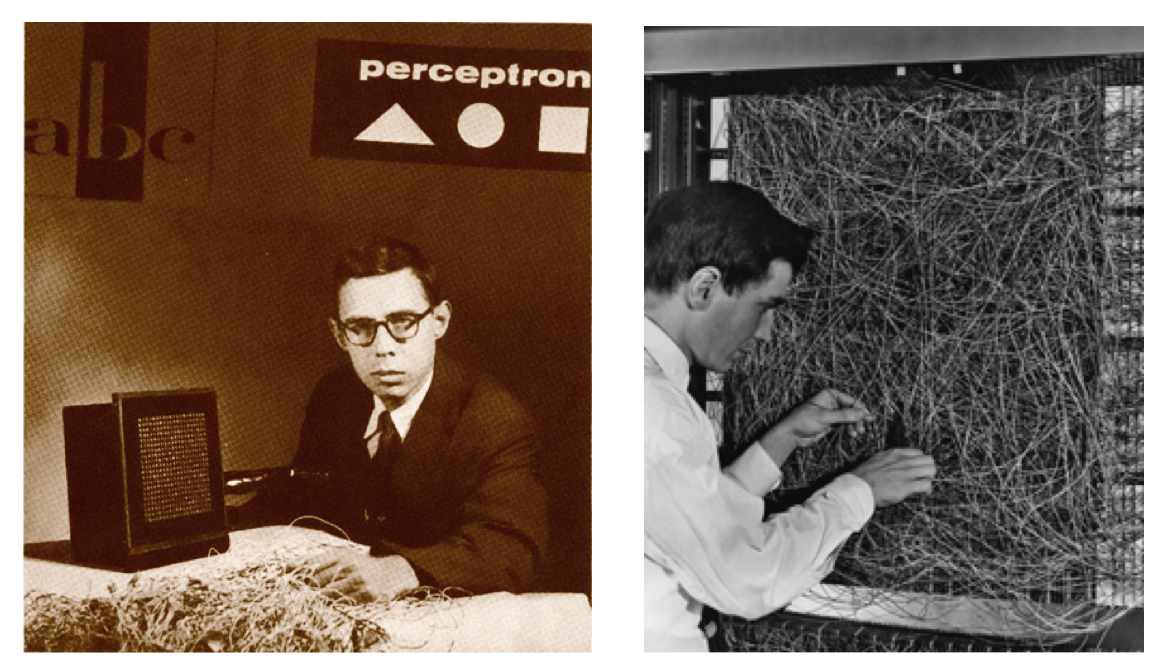
\includegraphics[width=0.7\textwidth]{images/perceptron.png}
\caption[Left: \url{http://www.rutherfordjournal.org/images/TAHC_rosenblatt-sepia.jpg}; Right: \url{http://www.newyorker.com/wp-content/uploads/2012/11/frank-rosenblatt-perception.jpg}]{Rosenblatt with one of his hardware implementations of a perceptron (left) and another view of the perceptron (right). }
\label{perceptron}
\end{figure}

Rosenblatt was a psychologist interested in human and animal behavior and its neural basis.\footnote{As with McCulloch and Pitts, Rosenblatt's personal history is fascinating, and in some ways tragic. See the Cowan and Hecht-Nielson interviews in Talking Nets \cite{anderson2000talking}.} He studied feed-forward networks with one layer of fixed weights and another layer of adjustable weights that could be trained to classify images on small displays as, for example, triangle vs. square, or male vs. female. He implemented his networks using huge tangles of wires for synaptic links (see Fig. \ref{perceptron}). This was quite impressive at the time and got a considerable amount of press.\footnote{See \url{https://www.youtube.com/watch?v=cNxadbrN_aI}} His rule was an early form of supervised learning rule based on a few if-then rules: if a sample is misclassified, then if output was too high, strengthen the weights, otherwise weaken the weights.  Rosenblatt proved that perceptrons could find solutions to certain types of classification tasks in a finite time \cite{rosenblatt1962comparison}.\footnote{This is known as the ``perceptron convergence theorem.'' For an intuitive discussion see \url{https://www.cs.cornell.edu/courses/cs4780/2018fa/lectures/lecturenote03.html}.} Haykin, who refers to this as the ``classical period of the perceptron'', summarizes Rosenblatt's importance as follows:
\begin{quotation}
The perceptron occupies a special place in the historical development of neural networks: It was the first algorithmically described neural network. Its invention by Rosenblatt, a psychologist, inspired engineers, physicists, and mathematicians alike to devote their research effort to different aspects of neural networks in the 1960s and the 1970s. Moreover, it is truly remarkable to find that the perceptron... is as valid today as it was in 1958 when Rosenblatt's paper on the perceptron was first published.
\end{quotation}
% Use the crazy Skynet quote about what Rosenblatt thought his machines would achieve

Whereas Rosenblatt focused on psychological implications of the perceptron, Widrow and his colleagues had engineering applications in mind, like adaptive noise cancelling in telephone wires.\footnote{According to Widrow this technology is used in every modem in the world and is at the heart of the internet; see \url{https://www.youtube.com/watch?v=skfNlwEbqck}. Widrow also implemented his networks using a special electrical components called a ``memistor'' which Widrow designed himself, which allowed weight updates in hardware. ALl of this is demonstrated in the video.} In the hardware implementation shown in Fig. \ref{adaline}, the toggle switches control input node activations, the knobs control weight strengths, and the dial shows the activation of an output node.\footnote{For Widrow's personal recounting of the Adaline and its history, see his interview in \emph{Talking Nets} \cite{anderson2000talking}. Also see the videos referenced in the figure caption, and the discussion in section \extref{lms_rule}}

\begin{figure}[h]
\centering
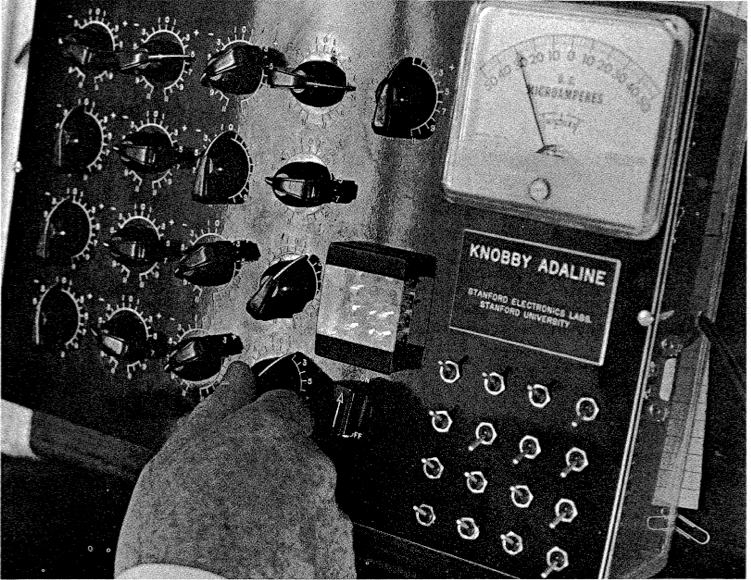
\includegraphics[scale=.3]{./images/adaline.png}
\caption[From \cite{widrow1963adaline}.]{A hardware implementation of Widrow and Hoff's ``Adaline'' network, which Widrow called the ``knobby Adaline'' on account of the prominent grid of knobs on the left, which control weight strengths, and which were manually adjusted to implement their learning algorithm. Inputs were produced using the 12 toggle switches on the lower right (and displayed in the grid of small lights), and the resulting output activation is displayed in the meter on the upper right. Videos of Widrow demonstrating the knobby Adaline, back in the 60s and also more recently, are available at \url{https://www.youtube.com/watch?v=skfNlwEbqck} and \url{https://www.youtube.com/watch?v=IEFRtz68m-8&t=161s}}
\label{adaline}
\end{figure}
% Show simbrain version

The least mean squares rule or LMS is discussed in section \extref{lms_rule}. Whereas Rosenblatt had derived his if-then rule from his understanding of biology, LMS was derived from calculus using first principles, which is how most modern learning rules are also derived. The essence of the rule is that we change each weight by a factor corresponding to the output error times the input node activation. This produces a kind of Goldilocks principle. When an output is too high (and the input is positive), we reduce the relevant weight so that the output will be lower, and  when an output is too low, we increase the relevant weight so that the output will be higher. In this way the network zooms in on the right value, so that the output is just right. This is, in a nutshell, the essence of how most modern neural networks work!  Widrow can be seen using this rule to train his machine to respond to T's and J's in variations positions in the video referenced in the figure caption. 

\section{The ``Dark Ages''}\label{dark_ages}

% Haykin points out the issues were part psychological, part financial. And other stuff. See p. 40
% Mention the convergence theorem itself
% Neocognitron, which anticipates deep learning. Done in industry. It's also a lot like pandemonium
% Sharai - We need references for Kohonen, Anderson, Braitenberg, Grossberg, and Carpenter.
% More on RL
% Compare the well-known AI winter, happened in another area but similar. Cf. Mitchell. Advised not to mention "AI" on her cv when she was on the market

Perceptrons and Adalines created a surge of interest in neural networks in the 1960s, but this was followed by a period of relative quiescence in the 1970s and 1980s, during what have been called the ``dark ages'', ``quiet years'', ``drought'', and ``winter'' of neural networks.\footnote{See PDP vol 1, ch. 1 \cite{rumelhart1986parallel}; Haykin p. 43 \cite{haykin1998neural}; Fausett p. 24 \cite{fausett1994fundamentals}. A variety of perspectives on the period are discussed in Talking Nets. 110, 155, 254, 305, 371. Grossberg, Carpenter, Kohonen, Anderson and others active in this period have their own interviews in Talking Nets \cite{anderson2000talking}.}  The dropoff in interest has been attributed to several causes. A key part of the story was that networks with a single layer of adjustable weights were shown by Minsky and Papert to suffer certain fundamental limitations \cite{minsky1969perceptrons} (see chapter \extref{ch_supervised}). So it was thought that neural networks weren't powerful enough to do psychologically realistic things. Moreover, at precisely that time more symbolic AI models were flourishing. 

However, even if interest in neural networks waned for a time, especially in comparison to AI, neural network research was active in this period. Relevant researchers include Kohonen, Amari, Fukushima, Anderson, Sutton, Barto, Braitenberg, Schmidhuber, Grossberg, and Carpenter. These and others laid the foundations for many of the ideas described in this book. So the dark years really weren't that dark.\footnote{Debates about the status of neural networks in this period are covered in some detail in Talking Nets \cite{anderson2000talking}.} 
% Mention that Fukushima worked on early deep networks. Say a bit about the others too, at least in a footnote

\section{First Resurgence: Backprop and The PDP Group}\label{first_resurgence}

% This section needs to be enhanced. This is where we get the cog-sci stuff. It's what the book is supposed to be about. Refer back to Bain and Freud's hopes. This flashes by currently. OR at least refer back to the material in ch. 1 which does some of the work.

% See the connectionists email about the history of backprop, and all the discussion in talking nets. Clearly Werbos should be discussed, but there were others too.
% Sharai - We need a reference for the discovery of backpropagation algorithm (is discovery in reference to it's creation or it's first application in neural networks?).
Connectionism came out of its (allegedly) dark decade and enjoyed a resurgence in the 1980s, for several reasons. Prominent among these was the discovery of the backpropagation algorithm, which overcomes the limitations associated with perceptrons. This makes it possible train networks with more than one weight layer, which in turn allows them to solve more complex problems (for example, ``linearly inseparable'' classification tasks; see chapter \extref{ch_supervised}) by developing internal representations. A simple example of this is the ability to train a network to solve the exclusive or (XOR) logic gate. McCulloch and Pitts neurons could be hard-wired by hand to solve this problem, but no one could train a network automatically to solve it, because it requires an additional layer of processing. This is easy to see in Simbrain: you can easily build an XOR network by hand (appendix  \extref{ch_logicgates}), but try to use LMS to train a one weight layer network on the same problem and the error will never go to 0. 

The internal representations discovered in many-layered networks using backprop were shown to have important properties both for engineering applications and for psychological theories, as we will see throughout the book.\footnote{In future iterations we hope to expand this section with a summary of some of the major work that began in this era, primarily in connectionism, using neural networks to model psychological phenomena. As a first note in this direction, we refer to the table at the end of this paper: \url{https://link.springer.com/article/10.1007/s42113-020-00081-z/tables/1}.}

%The competing program of symbolic AI was running into problems \cite{dreyfus1992computers}. 

A related reason for this renewed interest---particularly among cognitive scientists---was the publication of a major two-volume work in the period, {\em Parallel Distributed Processing: Adventures in the Microstructure of Cognition}, in 1986, by David Rumelhart, James MClelland, and the ``PDP research group'' (a group of researchers, many of whom were at UC San Diego.)  This publication brought connectionist networks back to the forefront, by clearly articulating the connectionist standpoint, showcasing a number of models of various aspects of cognition, demonstrating how to interpret the internal states and representations of neural network models of cognition, and clarifying how connectionist networks differ from symbolic AI models \cite{rumelhart1986parallel}. John Hopfield's models of associative learning in recurrent networks (i.e. ``Hopfield nets'', discussed in chapter \extref{ch_unsupervised}) were also influential in this period, in part because Hopfield presented his work in an especially clear, mathematically precise way.\cite{hopfield1982neural}\footnote{In Talking nets, on the PDP group, see pp. 180, 254, 277, and 281. On  backprop and its history, see pp. 286, 327, and 338. On Hopfield, see 113, 301 \cite{anderson2000talking}.}

% From Smolensky 1988: ``In the past half-decade the connectionist approach to cognitive modeling has grown from an obscure cult claiming a few true believers to a movement so vigorous that recent meetings of the Cognitive Science Society have begun to look like connectionist pep rallies''

% Net-talk was huge. See Talking Nets 324. I have material on this for other classes. Also Sejnowski is an important figure and should be mentioned.

\section{Second Decline and Second Resurgence: Convolutional Networks}\label{deep_revolution}

% Add reference to data science book that describes this sentiment. Maybe also that automatic diff video
For a time (roughly the late 1990s through about 2010), neural networks declined in interest as attention shifted to machine learning algorithms (cf. chapter \extref{ch_intro}). The problem was, in part, that tuning the parameters of a neural network seemed more an art than a science, especially when compared with machine learning, which is based on more tractable statistical principles. There was a sense that people just ``twiddled''  the knobs of a simulation as best they could until they got decent performance out of their network. In 2010 (in the midst of this decline), Phillip Jannert said: ``Neural networks were very popular for a while but have recently fallen out of favor somewhat. One reason is that the calculations required are more complicated than for other classifiers; another is that the whole concept is very \emph{ad hoc} and lacks a solid theoretical grounding'' \cite[Ch. 18]{janert2010data}.  There was a pervasive sense at the time that ``...neural nets were janky and did not work very well. They were seen as a hassle to work with---the computers were not fast enough, the algorithms were not smart enough, and people were not happy'' \cite{kurenkov2020briefhistory}.

However, several things happened that brought attention back to neural networks. First, larger datasets for training neural networks became available (what is sometimes referred to as ``big data''). Second, higher performance hardware for parallel neural network computing emerged, in particular using the graphical processing units or GPUs on graphics cards (the kinds used to play modern graphics intensive video games) and in proprietary hardware such as Google's tensor processing units (TMUs).\footnote{It is interesting that these games require lots of parallel processors to render texture and shading in real-time graphics processing using linear algebra (cf. chapter \extref{ch_linear_algebra}), and that the same parallel processing circuits can be used to run neural networks. When graphics cards were first developed they did not have neural networks in mind!} These breakthroughs suddenly allowed for the deployment of much larger \glossary{deep networks}. They not only had more layers, but relied on new, more complex, architectures.

Among these new architectures the most important were convolutional neural networks or CNNs (see   chapter \extref{ch_cnn}), which comprise sequences of convolutional layers, a special kind of weight layer in which a single set of shared weights is “scanned” over an input layer. Convolutional layers make it possible to effectively train deep networks with many more than 3 node layers.  CNNs led to an explosion of interest in deep learning and deep networks. Rather than only dealing with vectors and matrices, these architectures began to use more complex tensors (see \extref{sect_tensors}), such as ``volumes'' of activation describing images, videos, and other structures in rich detail.  Whereas most neural networks through the 1990s had just three simple node layers, CNN's can have tens or hundreds of layers, many of them multi-dimensional arrays. Thus networks with  a great deal of representational width and representational depth could be developed (see section \extref{structureNets} and chapter \extref{ch_cnn}). These many-layered convolutional networks existed as far back as the 1970s (via Fukushima's neocognitron and related models), but it is only in the 2010s  that a variety of technical hurdles relating to this type of network were surmounted. Indeed some have described the period beginning around the 2010s as a deep learning revolution, or as the decade of deep learning.\footnote{Andrey Kurenkov's history (\url{https://www.skynettoday.com/overviews/neural-net-history}) is excellent on these points. The achievements after 2010 are too numerous to survey here, but see \url{https://bmk.sh/2019/12/31/The-Decade-of-Deep-Learning/}.}  

\section{The Age of Generative AI}\label{age_generative_ai}

In 2017 Google introduced the \textbf{transformer architecture}---discussed in chapter \extref{ch_transformers}---which was subsequently adopted and extended by Open AI and many other groups in academia and industry \cite{vaswani2017attention}. The power of this architecture became widely known with the public release of Open AI's ChatGPT in 2022. ChatGPT had the fastest adoption rate of any software in history, and marked another shift in the history of neural networks and AI broadly. In this period, it became common to train extremely large models on vast amounts of data, using innovative new architectures like the transformer architecture. The resulting neural networks could be used to generate convincing outputs in multiple modalities, but especially text, video, and audio, hence the term \glossary{Generative AI}.\footnote{One mark of the shift is that it became extremely \emph{expensive} to train state-of-the-art models, and so reseachers could not train their own but had to rely on models trained by large companies such as Google, Open AI, and Microsoft.}$^,$\footnote{Though the term generative ``AI'' is used, this usually means \emph{neural networks} that have been used to generate these outputs, so this could more accurately be called ``generative neural networks'', but the term generative AI has stuck (see the first footnote in chapter \extref{ch_intro}).}

The transformer architecture builds on several streams of prior work. It is coming right off all the advances in training deep networks just discussed. They make use of huge datasets and benefit from innovations in hardware design.\footnote{As evidence, consider the explosive growth of NVIDIA, which started off in the graphics card business but is now a major driver of generative AI.} They develop many layers of internal representations that have a great deal of context awareness, which they can use to (for example) represent relationships between different parts of a fairly long conversation. The details are discussed in chapter \extref{ch_transformers}. The main initial use of transformer models was to generate natural language, and indeed ChatGPT is an example of a \glossary{large language model} (LLM), which is a language model trained on a large dataset--for example, a significant portion of text on the internet--to generate human-like text.\footnote{In fact, the terms ``transformer'' and ``llm'' have become conflated, though they are distinct (more on this in chapter \extref{ch_transformers}).}  The text produced by these models is now so convincing that they (in some contexts) pass the \glossary{Turing Test}, producing outputs that are not distinguishable from what a human can produce. Related advances (e.g. diffusion models) produce convincing images, videos and audio. 
% Matthew L: The interplay between the software and hardware innovations has been really cool to watch, with software (games) demanding certain kinds of hardware acceleration (GPUs), in turn enabling new kinds of software (large networks), causing new development in hardware (TPUs), in turn enabling bigger and more complex networks (transformers), that again then shaping the next generation of hardware (simpler operations with much higher parallelism and access to large amounts of memory with high bandwidth), in turn leading to... We'll see

These changes in the landscape of neural network research are significant enough that we are dubbing this the ``age of generative AI'' (the histories are just now being written, after all). This was when AI could really start generating new content, like news stories, essays, songs, images, and movies. In the future this will probably be seen as a landmark event, because this is when all the old doubts about neural networks were in a sense put to rest (of course, debate continues, but neural networks have clearly moved to the center of discussion), and when neural networks began to lead to fundamental changes in human existence, that we have not yet come to terms with.\footnote{This was also when ``artificial general intelligence'' (AGI) started entering the public consciousness, that is, AI that is not just able to do specific things in specific domains, but could behave in an intelligent manner in multiple domains and contexts. It is not generally believed AGI has been achieved as of yet.}

It has been a strange but exciting experience writing different versions of this chapter over the last few decades (the first version was written around 2005; see the Preface) as neural networks were out of vogue, then back in style, and then, arguably, completely transformed human society. No doubt more revisions to this chapter are coming, as the landscape continues to evolve.

%\chapter{Basic Neuroscience}\label{ch_neuro}
\chapterauthor{Jeff Yoshimi, Chelsea Gordon, David C. Noelle}{.4,.4,.2}

% Talk about inhibitory/excitatory ratios.   Esp since the sparse connectivity thing.  Also http://www.scholarpedia.org/article/Balance_of_excitation_and_inhibition which has this line, which begins to resolve the mystery a bit; “The possibility of excitation and inhibition having a comparable strength might seem implausible at first, since interneurons comprise only 15% - 25% of the population of cortical neurons. However, the synaptic strength and firing rates of inhibitory interneurons are substantially higher than in excitatory neurons, thus inhibitory interneurons have an impact disproportionate to their relatively small number.”
% A pass using neuroscience categories like precuneus, sfg, ifg, that show up frequently in  imaging based studies.

% https://cs.stanford.edu/people/karpathy/convnetjs/ interactive. but find something better

In this chapter, we review the basic physiology of neurons and synapses, which are the basis of equations describing how node activations and weight strengths change. We also provide an overview of the major circuits of the brain, reviewing their basic features, and giving a sense of how these circuits are understood from a neural networks standpoint.\footnote{Some useful general references include Kandel (2000) \cite{kandel2000principles} and Gazzaniga (2002) \cite{gazzaniga2002cognitive}. An outstanding online source is \url{https://science.eyewire.org/home}. A detailed book length treatment of the topics outlined in this chapter is \cite{cecn_4e}, which has also been developed into a free online text supported by open source software: \url{https://compcogneuro.org/}.}  

\section{Neurons and synapses}\label{neuronsSynapses}

\subsection{Neurons}

Neurons are brain cells, which have all the machinery any cell has: mitochondria, Golgi apparatus, a nucleus whose DNA is actively expressing genes, and a membrane studded with an array of proteins. Neurons communicate using a finely orchestrated pattern of electrical, chemical, and molecular processes. Neural network models typically abstract from most of these details. Classical neural network models only simulate certain high level features of the way information is transmitted from one neuron to another. Models in computational neuroscience (described in chapter \extref{ch_intro}) capture more of the biological details, but still abstract away from many features of real neurons. In the next two sections we give a rudimentary overview of the structure of neurons and synapses, focusing on features that are commonly referenced in neural network models.

\begin{figure}[h]
\centering
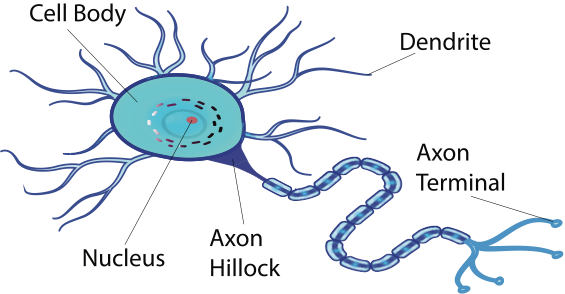
\includegraphics[width=.5\textwidth]{./images/neuron.png}
\caption[Pamela Payne.]{Main structures of a neuron.}
\label{f:neuron}
\end{figure}

% Possibly add discussion of myelin sheath, fast cortico-cortical communication, and white vs. gray matter
Most neurons have dendrites, axons, and a cell body (see Fig. \ref{f:neuron}).\footnote{There are many types of neurons in the brain, but in this section we focus on the \emph{multipolar} neuron. This type of neuron has one axon and multiple dendrites, which allows it to receive information from many other neurons. Other types of neuron include unipolar and bipolar neurons.}  These are not really distinct structures, but are parts of the cell. The neuron as a whole is a kind of container, whose overall charge is changing constantly over time like a fluctuating battery or capacitor. 

\glossary{Dendrites} are extensions that grow out of the cell body like a tree (``dendrite'' comes from a Latin word that means ``tree''). This is where information-carrying chemicals are received from other neurons. Dendrites have small branches, which can receive signals from many other neurons. Some metaphors might help you remember this: You can think of a dendrite as the mail-box of a neuron, receiving messages from many nearby cells. You can also think of it as a catcher's mitt, since it receives or ``catches'' inputs from other neurons.

% Maybe say more about what's happening in the cell body. Expressing genes to produce and package and transport neurotransmitter, for example. Just a flavor of how active it is. 
The cell body or \glossary{soma} is home to many organelles that work to produce and package proteins for the cell. These proteins have a variety of important functions, including the production of neurotransmitters that signal between cells. The soma sums together all the information gathered from the dendrites. If the voltage changes enough at a part of the soma called the \emph{axon hillock}, the neuron will fire an \glossary{action potential} or spike along its axon. We expand on these ideas in the discussion of synapses next. 
% [Merge or make footnote] These chemicals are called \glossary{neurotransmitters}. These messages (neurotransmitters) attach themselves to \glossary{receptors} on the dendritic branches. Different types of neurotransmitters have different binding sites on the dendrite. Once attached, these chemical messages trigger the electrical transmission of ions throughout the rest of the cell. The particular message carried by a neurotransmitter is important for determining what happens inside of the cell once it binds, and we will discuss a bit later what these different types of messages are. Importantly, this transmission changes the voltage of the cell as a whole, and as we will see, this voltage change is an important  component of within-neuron communication.

The \glossary{axon} is another extension growing out of the cell body. Axons can be different lengths, but they often have a long main extension terminating in a branched structure. When the neuron fires an action potential, electrical activity propagates down these extensions and triggers the stimulation of the dendrites of other neurons. Continuing our metaphors: the terminals at the end of the axons can be thought of as a neuron's post office, where the ionic messages transmitted down the axons are packaged into neurotransmitter chemicals and sent out on their route to the receiving neuron's dendrite. Or, continuing the baseball metaphor, the axon is like the arm of a pitcher, throwing signals to other dendrites, which catch them.\footnote{Fast communication between long-distance neurons is made more efficient by a fatty white substance, called \emph{myelin sheath}, that wraps around the axons of neurons and insulates them, allowing better conduction of electrical signals}

% Mention Simbrain and all the neuron models it contains. Point ahead to next chapter.

\subsection{Synapses and neural dynamics}\label{simpleNeuralDynamics}

Communication between neurons happens at a \glossary{synapse}, which is a junction where the axon of the \emph{pre-synaptic} neuron almost touches the dendrite of the \emph{post-synaptic neuron}, often at a protrusion called a \emph{dendritic spine}. See Fig. \ref{f:synapse}.\footnote{There are two types of synapses, electrical synapses and chemical synapses. Electrical synapses, instead of having a cleft between the post- and pre-synaptic neurons, have a much smaller space called a \emph{gap junction}, which connects the pre-synaptic neuron directly with the post-synaptic neuron, allowing for electrical communication. These synapses allow neurons to fire in synchrony and are important for quick communication between neurons. However, most communication happens via chemical synapses, which transmit much stronger signals and have more permanent effects. The main text focuses on chemical synapses.}  When an action potential reaches the axon terminal of the pre-synaptic neuron, chemicals called \glossary{neurotransmitters} are released into the synaptic cleft. These neurotransmitters are housed in water-balloon-like containers called \emph{vesicles}. The vesicles fuse into the pre-synaptic cell membrane when an action potential occurs, releasing their neurotransmitters into the synaptic cleft. The neurotransmitters then bind to \glossary{receptors} on the post-synaptic neuron. This is like a key being fit into a keyhole--the neurotransmitters are the keys and the receptors are the keyholes which, when opened, let ions (charged particles) flow in to the post-synaptic dendrite. These ions are negatively or positively charged, and the balance between the total charge of these ions on either side of the cell membrane is what is called the \glossary{membrane potential}.\footnote{This charge is maintained by ion channels that selectively let some ions travel into and out of the cell. Some of these ion channels are called \emph{passive ion channels}, which stay open and allow the constant light flow of Na$^+$ and K$^+$ ions through the cell membrane. There are also \emph{gated ion channels}, which are those that open during an action potential and cause a much larger exchange of ions. When these open, the ions released cause changes in the membrane potential of the post-synaptic neuron.}

\begin{figure}[h]
\centering
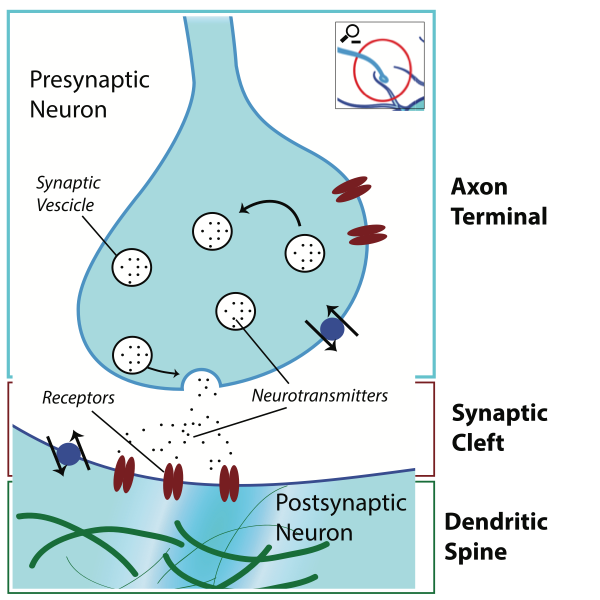
\includegraphics[width=.45\textwidth]{./images/synaptic_cleft.png}
\caption[Pamela Payne.]{Some structures associated with a synapse.}
\label{f:synapse}
\end{figure}

There are different kinds of synapses. The pre-synaptic neurons of  \glossary{excitatory synapses} release neurotransmitters, which result in the  post-synaptic voltage being raised, which makes it more likely that an action potential will occur post-synaptically. \emph{Glutamate} is one of the most common excitatory neurotransmitters. \glossary{Inhibitory synapses} release neurotransmitters, which result in the voltage being lowered post-synaptically, and make it less likely that an action potential will occur post-synaptically. \emph{GABA} is the most common  inhibitory neurotransmitter.

\begin{figure}[h]
\centering
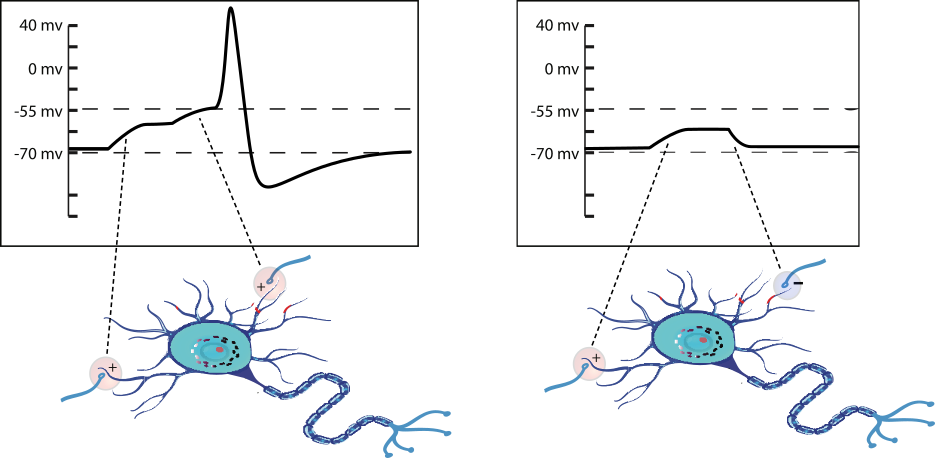
\includegraphics[scale=1.5]{./images/membranePotential3.png}
\caption[Adapted from original work by Pamela Payne.]{(Left) Two successive excitatory inputs increase the neuron's membrane potential beyond the threshold potential, after which it fires an action potential. (Right) First an excitatory input increases the neuron's membrane potential, then an inhibitory input reduces it. }
\label{membranePotential}
\end{figure}
% Make blue darker

A neuron can receive both excitatory and inhibitory inputs.\footnote{What we are calling excitatory and inhibitory inputs are actually synaptic events that allow ions to rush in or out of the cell, and thus produce excitatory or inhibitory currents. From this standpoint the neuron is like a battery or capacitor and its membrane dynamics can be understood in terms of circuits (the ``Rall model'' or ``cable theory'' of the neuron), which can be precisely described in computational neuroscience models. The membrane potential has an average resting state, usually around -70 mV, which is the difference between the electrical charge inside and outside of the membrane when a neuron is at rest. Excitatory and inhibitory inputs alter this resting state. One metaphor that helps here is that of a tank of water or a graduated cylinder, where the level of water represents the current voltage potential. There is a hole on the side of the tank that constantly lets some water out, and a tube above it that constantly lets some water in. These produce a ``leak'' current that balances out to a certain standing level in the tank, which is like the resting potential of a cell. That level is roughly where the hole on the side of the tank is. Excitatory inputs briefly open up additional tubes above the tank, letting more water in and raising the water level (the membrane potential), and inhibitory inputs briefly open up additional tubes below the tank, letting more water out and reducing the water level. These transient events lead to fluctuations in the water level which correspond to sub-threshold dynamics of the membrane potential.} As different axons attaching to a neuron release excitatory neurotransmitters (like glutamate) and inhibitory neurotransmitters (like GABA), the binding of neurotransmitters to receptors on the post-synaptic neuron causes ion channels to open and close, letting different ions in and out. As a result, the neuron's voltage goes up and down. When the voltage at the axon hillock passes a specific membrane potential called the \glossary{threshold potential}, an action potential is fired. The process is illustrated in Fig. \ref{membranePotential}. In the left panel, two excitatory synapses are activated successively, and the membrane potential is increased each time until it passes the threshold potential and an action potential is fired.\footnote{Notice the signals occur at spatially distinct dendrites and at different points in time, and that they have a cumulative effect on the membrane potential at the soma. This is known as \emph{spatial and temporal summation}.}  In the right panel, first an excitatory synapses is activated, which raises the membrane potential, and then an inhibitory synapse is activated, which reduces the membrane potential, in effect turning off or ``shunting'' the impact of the first excitatory input, so that no action potential occurs. Changes in membrane potential due to excitatory and inhibitory events that occur below threshold are sometimes referred to as sub-threshold dynamics.

As more excitatory signals are received, the membrane potential will exceed the threshold potential more often, and action potentials will begin to occur more frequently. Thus we can represent the overall activity of a cell in terms of its \glossary{firing rate}, which is measured in number of spikes per unit time, usually spikes per second. A highly ``active'' neuron is one that produces many spikes per second (e.g. 200 Hertz, which is 200 times per second), while a more dormant or quiescent neuron might only produce a few spikes per second (e.g. 2 Hertz). In a time series plot of such a neuron's membrane potential, spikes for a highly active neuron are close together; for a less active neuron they are farther apart. You can get a feel for this in the Simbrain simulation  \emph{spikingNeuronTwoInputs.zip}. In the simulation you can increase the firing rate of the neuron on the left by raising the excitatory input. You can then reduce its firing rate by raising the inhibitory input. See figure \ref{twoNeuronsSpiking}.
  
 \begin{figure}[h]
\centering
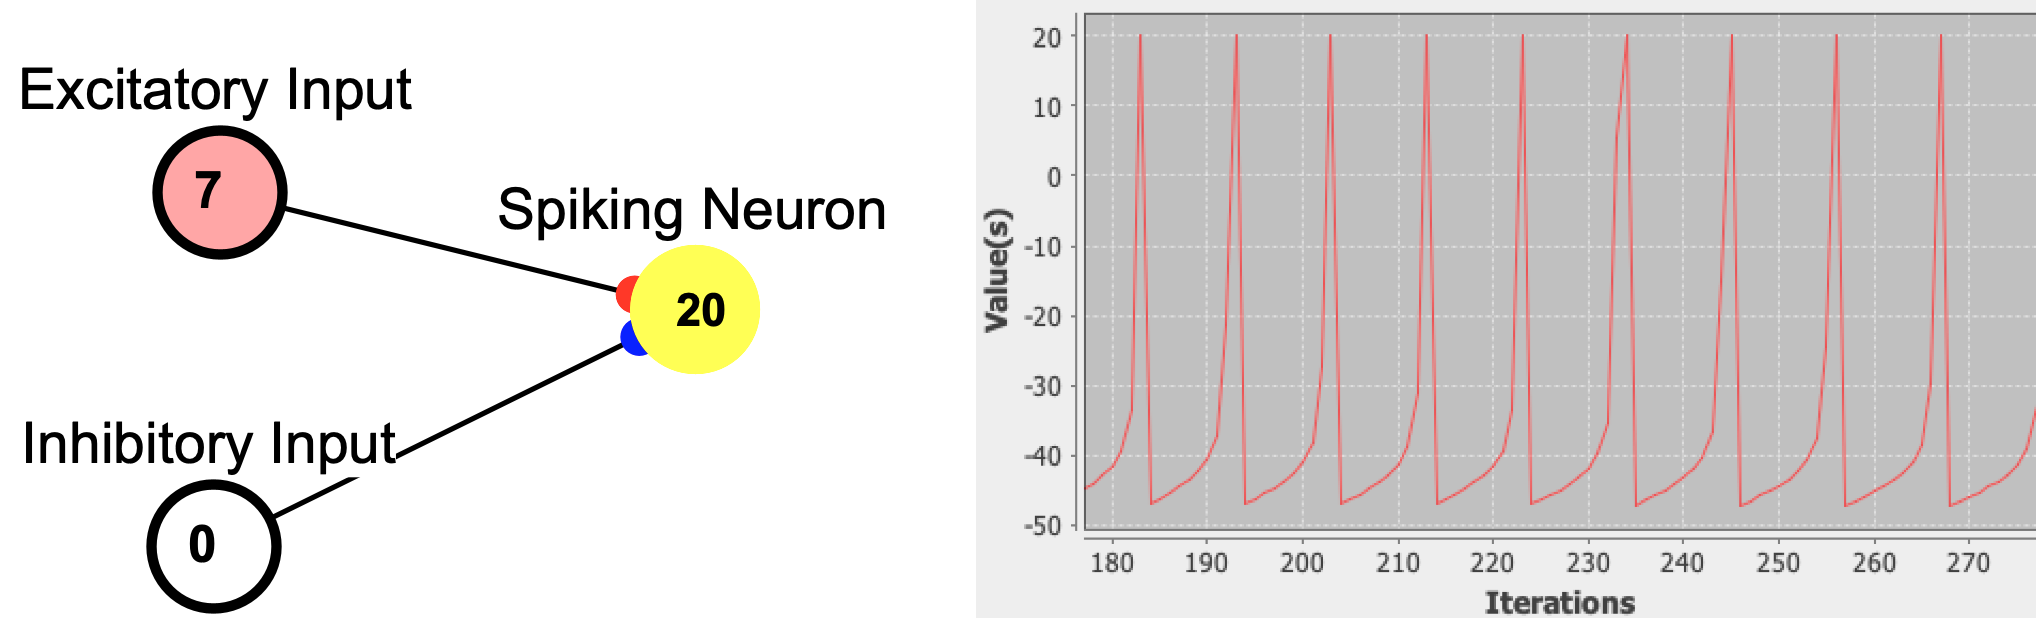
\includegraphics[scale=.4]{./images/TwoNeuronsSpiking.png}
\caption[Jeff Yoshimi.]{(Left) A Simbrain simulations that illustrates how different combinations of excitatory and inhibitory inputs produce different firing rates in an output neurons. As the excitatory input is increased, the firing rate increases, and as inhibitory input is increased, the firing rate decreases. The output neuron is in the middle of a spike at the moment shown. }
\label{twoNeuronsSpiking}
\end{figure}
% The rate coding idea that the number _represents_ that rate is not yet clear, but not sure how much an be done here

These observations are the basis of ``rate-coding'' models. In these models, the number in a node represents a neural firing rate. Weights in these models capture the idea the neuron sums together excitatory and inhibitory signals. Rate coding is in the background of many connectionist models, where much of the biology is abstracted away and all that is maintained is the general idea that a weighted sum of inputs determines the output of a node.  More complex computational neuroscience models describe the changing membrane potential directly, or simulate the action potential using discrete spiking events (see chapter \extref{ch_spiking}). These models are discussed in the chapter on computational neuroscience and in the chapter on classical nodes and weights.

Synapses are modifiable. For example,  \glossary{Long Term Potentiation} or LTP occurs when certain synapses transmit information repeatedly in a short time. When this happens the synapse is ``strengthened'': when an action potential reaches the same synapse after LTP has occurred, the post-synaptic response will be greater than it was before.\footnote{The details of LTP are not well understood, but roughly what happens is this: the repeated stimulation of the post-synaptic neuron results in an influx of calcium ions, which has a number of effects. One is the recruitment of additional receptors to the post-synaptic dendrite, so that when neurotransmitters are subsequently released into the synaptic cleft more receptors open and more ions are allowed into the post-synaptic cell.}   Long term potentiation is the basis of the Hebb rule, discussed in chapters \extref{ch_history} and \extref{ch_unsupervised}. The basic idea of the Hebb rule is that ``neurons that fire together, wire together.''\footnote{This can be visualized in several Simbrain simulations, for example \emph{autoassociator1.zip} and \emph{autoassociator2.zip} in the courseMaterials directory.}   

Synapses can be modified in other ways. Sometimes synapses are weakened via a process of \emph{Long term depression} or LTD. Synapses can be modified in other ways as well, and the study of synaptic plasticity is a major area of research. These changes in synaptic efficacy are thought to be the basis of most forms of learning in humans and animals. The idea that changing connection strengths are the basis of learning is what gives ``connectionism'' its name, and is fundamental to neural network theory.

\subsection{Neuromodulators}\label{neuroModulator}

% https://www.ncbi.nlm.nih.gov/pmc/articles/PMC5807333/
% The cerebrospinal fluid (CSF) occupies the brain’s ventricles and subarachnoid space and, together with the interstitial fluid (ISF), forms a continuous fluidic network that bathes all cells of the central nervous system (CNS). As such, the CSF is well positioned to actively distribute neuromodulators to neural circuits in vivo via volume transmission. Recent in vitro experimental work in brain slices and neuronal cultures has shown that human CSF indeed contains neuromodulators that strongly influence neuronal activity. 

We mentioned GABA and glutamate above. These are neurotransmitters that support local communication from one neuron to another. Other neurotransmitters---which are sometimes called ``neuromodulators''---are connected with circuits that project across larger regions of the brain and have longer-lasting impacts.\footnote{On the relationship between neurotransmitters, neuromodulators, and neurohormones  ``A neurotransmitter is a messenger released from a neuron at an anatomically specialised junction, which diffuses across a narrow cleft to affect one or sometimes two postsynaptic neurons, a muscle cell, or another effector cell. A neuromodulator is a messenger released from a neuron in the central nervous system, or in the periphery, that affects groups of neurons, or effector cells that have the appropriate receptors. It may not be released at synaptic sites, it often acts through second messengers and can produce long-lasting effects. The release may be local so that only nearby neurons or effectors are influenced, or may be more widespread, which means that the distinction with a neurohormone can become very blurred. A neurohormone is a messenger that is released by neurons into the haemolymph [or, in mammals, into the blood] and which may therefore exert its effects on distant peripheral targets.'' \cite{burrows1996neurobiology}.}   Some neural network simulations model the effects of these neurotransmitters.

\emph{Norepinephrine}, or noradrenaline, is produced by neurons in the brainstem and broadcast throughout the brain. It regulates arousal: there is a greater amount of norepinephrine when awake and a decreased amount while asleep. 

\emph{Serotonin} is also produced by cells in the brainstem. Serotonin is involved in attention and complex cognitive function. Low serotonin has been linked to depression. A type of medicine referred to as an SSRI (selective serotonin reuptake inhibitor) causes less of the serotonin released by cells to be taken back into the pre-synaptic neuron, so that more serotonin stays in the synapse and gets used. 

\emph{Acetylcholine}, found in motor neurons in the spinal cord, is responsible for movement and also mediates certain forms of plasticity. Too little acetylcholine can inhibit movement, while too much acetylcholine can cause twitching. Black widows inject a chemical in their bite that promotes the release of acetylcholine, which leads to severe muscle twitching.

\emph{Dopamine} is a neurotransmitter produced in the basal ganglia (in the ``nigrostriatal pathway''), which plays an important role in controlling movement. Shortage of dopamine in the system can lead to \emph{Parkinson's disease}, characterized by an inability to initiate movements. A drug called \emph{L-Dopa} can be used to stimulate the production of dopamine, which helps to even out dopamine levels and alleviate some of the symptoms exhibited by Parkinson's patients. Dopamine is also important in regulating the reward-based learning that occurs in the basal ganglia, which is discussed further below.  It is important to note that dopamine is \emph{not} a direct signal of reward (that signal is carried by other opioid-based circuits in the brain), but rather a signal of how much more or less reward than expected was obtained; a kind of error signal.  When things are going better than expected, dopamine neurons fire at an increased rate.  When things are going worse, they fire at a reduced rate. When you are not expecting a donut (assuming you like donuts and are hungry), the arrival of a delicious donut will cause dopamine neurons to start firing. But as you eat, even if you are still hungry, dopamine neurons stop firing, because your expectations are no longer changing.  On the other hand, if you were expecting those donuts when the door opened and you are disappointed to see that your friend forgot to bring them (oh the horror), your dopamine neurons will fire \emph{less} than normal. Thus dopamine is an important signal which can be used to train animals, by encouraging them to do things that lead to unexpected rewards, and by discouraging them from doing things which lead to unexpected disappointment. This signal is key to computational models of the  the basal ganglia, discussed below.
% 1)  Anticipating / wanting. That is due to dopamine. Seeing the cupcake. (2) The actual reward.  Opiods. Eating the cupcake. See Daniel Levitin 2022 talk notes and perhaps get the picture he used. 

\section{The Brain and its Neural Networks}

In this section we describe regions of the brain, functions associated with them (summarized in Fig. \ref{brain_lobes}), and give a sense of the computational role they serve in cognition and how they are modeled by neural networks.

It is worth noting at the outset that these associations between brain regions and cognitive functions are somewhat artificial. Most types of cognition are based on circuits that span multiple brain areas. Conversely, most areas of the brain are involved in  many kinds of cognition and behavior. For instance, motor regions of the brain are known to be active in body movements, but  also participate in movement planning, observation of the movements of others, and even the perception of objects that can be manipulated (i.e., grasped). Thus, when we talk about ``language areas'' or ``decision-making regions'', we are discussing regions that are active when the relevant behaviors occur, but these regions are not solely responsible for such tasks. In the same way that neurons work in groups to process information, higher brain areas work together to create complex thought and behavior.

\begin{figure}[h]
\centering
\raisebox{-0.5\height}{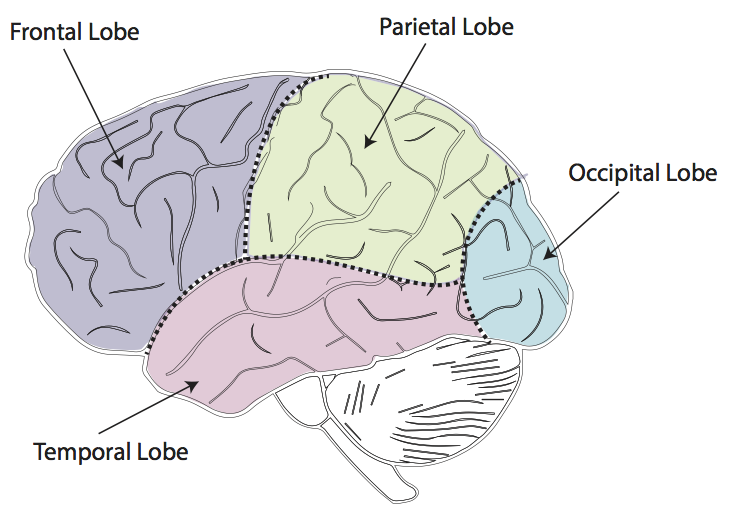
\includegraphics[width=.43\textwidth]{./images/brain_lobes.png}}
\hspace*{.2in}
\raisebox{-0.5\height}{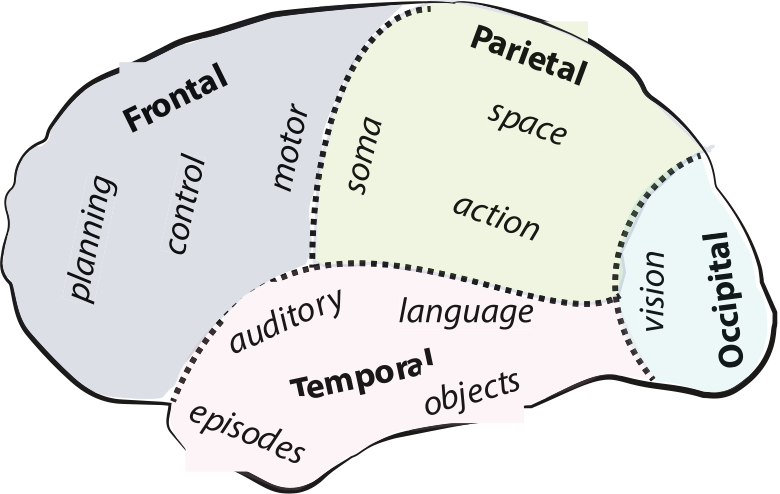
\includegraphics[width=.35\textwidth]{./images/brain_functions.png}}
\caption[Left: Pamela Payne; Right: Pamela Payne, using text taken from the Emergent Wiki.]{(Left) The lobes of the brain. (Right) Rough map of functions, abilities, and conceptual domains associated with major brain areas.}
\label{brain_lobes}
\end{figure}
% Right panel has a slight graphical error on top "dorsal" to the pic
% Add concrete/abstract, how -what, and an inset showing hot / cool, OFC, and ACC. Also redo 3.9 in a similar way

\subsection{Cortex}
% Link region discussions here with deep net chapter and the internal representations chapter

Fig. \ref{brain_lobes} (Left) shows the major regions of the brain. Fig. \ref{brain_lobes} (Right) summarizes the functions associated with these areas. These are regions of the \glossary{cerebral cortex}, which is the wrinkled outer surface of the brain (cortex literally means ``rind'', like the outer skin of an orange or lemon). The wrinkling is caused by the cortex folding, like a crumpled piece of paper, in the limited volume of the skull. This folding results in bulges (called ``gyri'') and valleys (called  ``sulcuses'' or ``sulci'') on the surface of cortex. The cortex is thought to be involved in the higher processing functions distinctive of complex behavior and intelligent animals. The size of an animal's cortex roughly correlates with the complexity of its behavior and overall intelligence: humans and dolphins have a relatively large cortex, chimps a smaller cortex, rats even smaller, and non-mammals like birds and insects have no cortex at all. The cortex is composed of two hemispheres, the right and the left hemispheres, connected by a structure made up of nerve fibers called the ``corpus collosum''. Between-hemisphere communication occurs through the corpus collosum. In patients with a neurological disorder called ``epilepsy'', where too much neuronal firing in the brain leads to seizures, the corpus collosum is often severed (this is called a ``collosotomy'') to reduce between-hemispheric communication and prevent future seizures. Both the right and left hemispheres are made up of the same lobes (occipital, temporal, parietal, and frontal).	

From a computational standpoint, the cortex is the brain's primary long-term memory system, which stores all the many things we know about the world: how we classify objects, our concepts, our beliefs, our memories, our knowledge about our friends and family, our life goals and fundamental cares, almost everything is coded into this massive memory system. Many neural network models are directly or indirectly simulations of our long-term cortical memory system. They model pattern recognition via learning, memory storage and recall, pattern completion, spreading activation, and many other phenomena. In fact, unless otherwise noted, most neural networks are probably ultimately models of how cortex works.
% Mention cortex model in Simbrain
%It is like your persistent storage system, but it is quite different from a computer's solid-state memory at all. In a computer, memory is distinct from processing, but in the brain, the same circuits that support memory also support processing.  There are many disanalogies. In general, it is a living, pulsing, plastic tissue, a network of millions of cells and billions of synapses that are constantly being incrementally updated.  

The cortex has dense bi-directional recurrent connections that allow it to reverberate in sustained patterns. It  also has long range connections between areas that allow it to produce complex brain-wide patterns or oscillations (though some circuits are also similar to feed-forward networks). In concert with the central thalamic relay station (more on this below), the posterior and parietal parts of cortex reverberate and coordinate sensory input and motor outputs when you engage in most behaviors. The frontal regions manage our plans and actions. Other circuits refine these signals, producing smoother movements (cerebellum), coordinating sequences of activations to produce reward (basal ganglia), and managing recent memories (hippocampus). Thalamo-cortical oscillations are correlated with consciousness. When you see something and are aware of it,  sustained processing in multiple cortical areas is  associated with your experience: visual activations are associated with visual awareness, activation in somatic areas is associated with awareness of your body, more distributed activations are associated with inner thoughts, etc. These are sometimes referred to as the neural correlates of consciousness or NCCs.
% Add NCC citation
% Summarize GNW vs. RPT and expand on consciousness discussion, with citations.
% Even those who deny this, like Solms, allow that they are correalted

Learning in this long-term memory store occurs via a mixture of unsupervised and supervised learning. Synapses are updated by LTP and other means,  which can be modeled using unsupervised learning algorithms like Hebbian learning and unsupervised architectures such as self organizing maps (see chapter \extref{ch_unsupervised}). One theory of cortex is that it is a giant collection of internal models in long-term memory: models of physical objects, the people you know, language, etc. These models learn from unsupervised methods, but they also come to have expectations about external inputs and inputs from other models. On this view, most processing in the cortex, and thus most of what we see and hear and understand, is based on what we \emph{expect}, based on our internal models of situations. The signals that flow through cortex are actually error signals--a kind of training signal--which  indicate how what we see differs from what we expect. Thus cortical networks incorporate elements of supervised learning (chapter \extref{ch_supervised}). This view, known as the ``predictive coding'' or ``predictive processing'' view, originates in part in computational models of visual cortex \cite{rao1999predictive}, but it has since developed into a more general view about the structure of perception and cognition and their realization in the brain \cite{clark2013whatever}.
% More citations. Free energy etc. Also clarify that this is controversial.
% Top down vs. bottom up effects in perceptions
% Link to IAC HW. Think of all the things you can encode in an IAC network. But problem is that's not unsupervised.

In many cortical areas there is a progression from areas that handle low-level sensory processing (e.g. edge detection in primary visual cortex, or tones in primary auditory cortex) to regions that handle more complex pattern recognition, like face recognition. The reverse direction is similar: high level plans are handled by more ``interior'' networks, while detailed motor movements are handled closer to the output layers of the cortex, that feed to thalamus and then to muscle systems. Thus, many cortical areas have a hierarchical structure, which is precisely what is modeled by deep networks. 
% Check and improve esp this paragraph

\subsection{The Occipital Lobe}

The \glossary{occipital lobe} and some of its features are shown in Fig. \ref{brain_vision}. Its most dominant feature is the \glossary{visual cortex}, which supports visual processing, including edge detection, color detection, and simple motion detection. Damage to the visual cortex can produce blindness (\glossary{cortical blindness}), even if the eyes are intact. Processing begins in the eye (in the retina, which is itself a complex neural network), and is then passed along to several structures, most prominently the visual cortex. Processing within the visual cortex occurs in a series of stages, which are thought to correspond to the extraction of increasingly complex features of a visual scene. For example, V1 and V2  process information about edges and form, V4 is involved in processing of color, and area MT plays a role in motion processing. 
% Mention Hubel / Wiesel?
% Add V4 since it comes up in deep networks?

\begin{figure}[h]
\centering
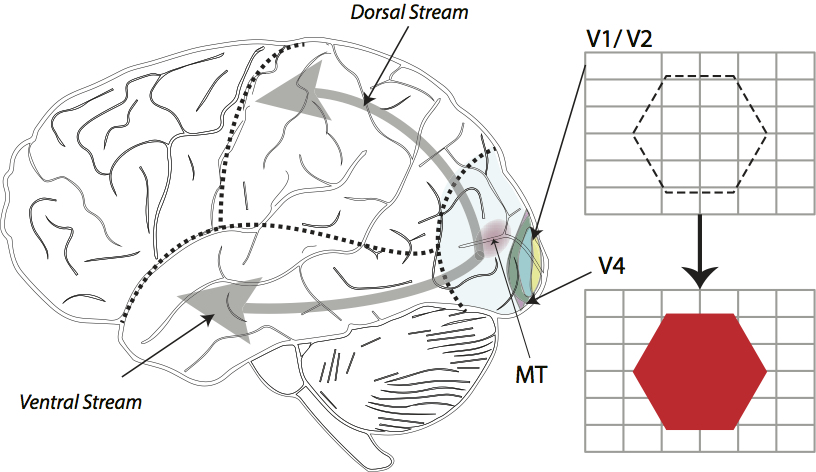
\includegraphics[scale=.6]{./images/brain_vision.png}
\caption[Pamela Payne.]{The visual cortex and associated structures.}
\label{brain_vision}
\end{figure}
% Add IT and FFA

% Clarify what a map is. Nearby firing neurons represent similar classes of inputs. Then use parallel constructions in discussion the other topographic maps.
Each of the regions of visual cortex contains something called a \glossary{retinotopic map}, which is a full neural map of locations in the retina, where groups of neurons nearest one another process information about nearby areas in visual space. More generally, a \emph{topographic map} is an area of the cortex where sensory information is processed in a spatially organized manner. We will see that multiple sensory regions contain topographic maps of their respective sensory information. In chapter \extref{ch_unsupervised} we will see that some neural network algorithms, like self organizing maps, can automatically produce banks of detectors that are topographically organized.

Information passes out of the visual cortex in two streams: a \glossary{dorsal stream} to the parietal lobe, which is involved in coordinating visual and spatial information, and a \glossary{ventral stream} to the temporal lobe, which is involved in processing complex visual features of objects and semantic knowledge, i.e. information about what things are  (see Fig. \ref{brain_vision}). We will discuss these pathways in more detail below.
% Object recognition is something many FF neural networks  do

% TODO: Replace with Yamins 2016.
% Also: "Two foundational empirical observations about cortical sensory systems are that they consist of a series of anatomically distinguishable but connected areas3,4 (Fig. 1b) and that the initial wave of neural activity during the first 100 ms after a stimulus change unfolds as a cascade along that series of areas2."
% In that paper IT / the ventral stream are divided into three subparts
\begin{figure}[h]
\centering
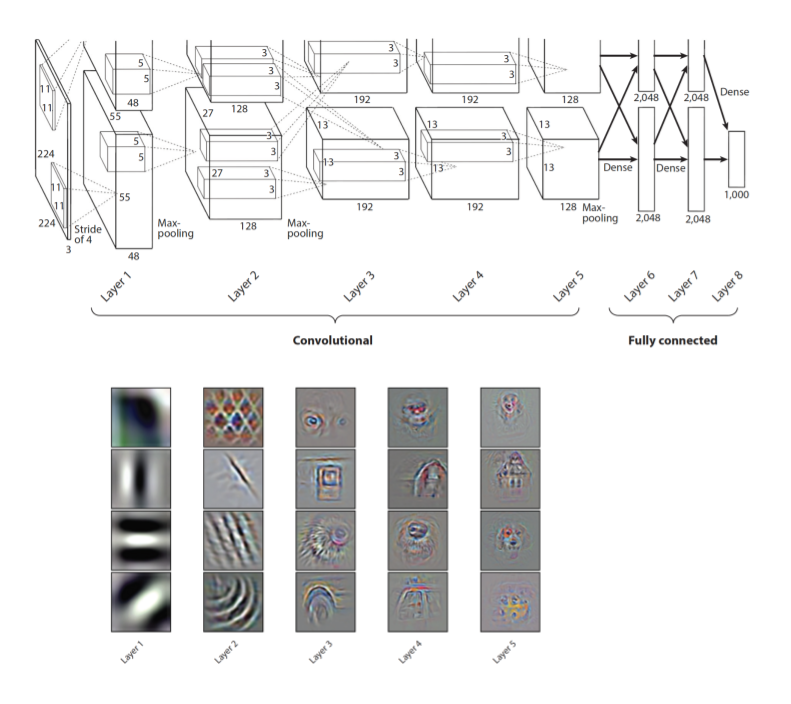
\includegraphics[scale=.4]{./images/deepLearningBrain.png}
\caption[From \cite{kriegeskorte2015deep}, which is in turn based on \cite{krizhevsky2012imagenet} and \cite{gucclu2015deep}.]{A well-known deep neural network architecture AlexNet (based on \cite{krizhevsky2012imagenet}) whose activations match those of actual brain areas. The top level shows the network architecture, and the bottom panel shows receptive fields (activations that maximally activate specific nodes) of a similar network \cite{gucclu2015deep}. Though these networks were developed as an engineering tool to classify images, they do a good job of describing neural activation in V1, V2, V4, and IT.}
\label{deepLearning_Vision}
\end{figure}
% This is misleading, because they are two networks. Also we need to get permissions.

It has emerged in recent years that deep learning networks are particularly well suited to describing what these areas of the brain do. These networks are trained to recognize images, which is a useful engineering application, but it turns out they do a good job of describing neural activity in the brain. For example, a well known deep network known as ``AlexNet'' \cite{krizhevsky2012imagenet} is shown in the top panel of figure \ref{deepLearning_Vision}. It develops topographic maps similar to those in the brain. The activations it produces at its various layers in response to images match the activations of the brain in response to the same images quite well. The earlier layers of the model mimic the response properties and receptive fields of lower levels of processing, like V1, and later layers mimic properties V4 and ventral stream neurons in IT. The exciting thing about these models is that we can produce pictures of their receptive fields, showing precisely what kind of input each neuron learned to respond to. As can be seen in the figure, lower level layers in this kind of network become edge detectors, further downstream layers respond to combinations of these features (compare Selfridge's demons from chapter \extref{ch_history}), while IT layers respond to dogs, cats, etc.\footnote{There has also been some skepticism about deep network approaches to human vision \cite{bowers2022deep}.}
% Principles apply in other brain areas

\subsection{The Parietal and Temporal Lobes}

% Clarify. Neurons are arranged spatially in a way that matches the arrangement of tones by frequency.
The \glossary{temporal lobe} is involved in auditory processing and semantic processing (see Fig. \ref{brain_audition}). The \glossary{auditory cortex} is in the temporal lobes. Much of the sensory information from the ears is sent to auditory cortex. Primary auditory cortex (A1) contains a \glossary{tonotopic map} of the acoustic properties of sounds. That is, neurons in this region respond to preferred frequencies of sound in a similar way to the preferred spatial regions in retinotopic maps. Auditory information is also processed in a somewhat hierarchical fashion, similar to vision. After A1, information passes to the secondary auditory cortex (A2), where sound localization and processing of more complex sound features occurs. When the auditory cortex is damaged, people can experience hearing deficits (they may suffer from ``central hearing loss'' or cortical deafness) even if the ears are intact. Other parts of the temporal lobe are involved in language processing. Wernicke's area, located in the temporal lobe\footnote{More specifically, the temporal lobe in the dominant hemisphere, which is usually the left hemisphere.}, plays an important role in speech understanding. This region is involved in assigning meaning to sounds. Damage to this area can produce \glossary{Wernicke's aphasia}, where patients are unable to understand either spoken or written language.
% Make cortical deafness a glossary item to match cortical blindness
% Some revision to bring out the sequence of processing centers

\begin{figure}[h]
\centering
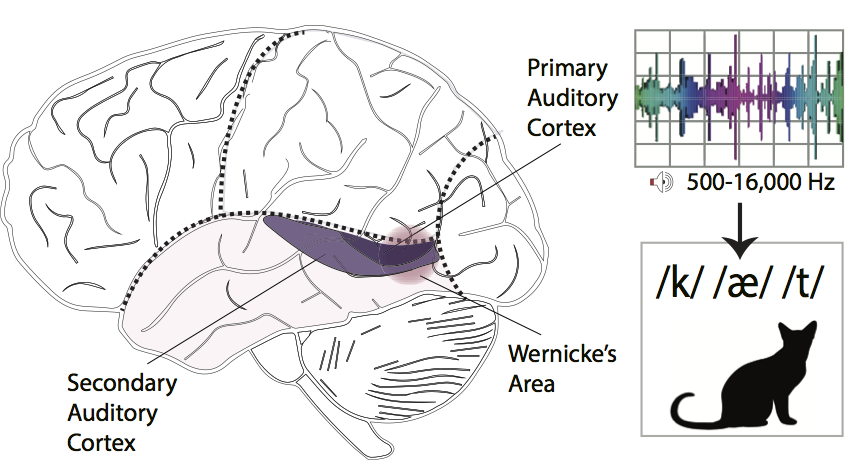
\includegraphics[scale=.7]{./images/brain_audition.png}
\caption[Pamela Payne.]{Auditory cortex and associated structures.}
\label{brain_audition}
\end{figure}
% Explain the phoneme symbols in the caption
% Add fusiform face area to image

The  temporal lobe also receives connections from the visual processing centers of the occipital lobe, via the ventral stream (Fig. \ref{brain_vision}). The ventral stream is involved in object recognition. For example, the fusiform face area (FFA) in the temporal lobes is connected with the recognition of faces. Damage to this region will cause \glossary{prosopagnosia}, an inability to recognize faces. It has since also been found that the FFA is active in bird experts while looking at birds and chess players while recognizing chess board configurations. This suggests that this region is involved in recognition of objects that one has expertise with \cite{boggan2011chess}. Another form of damage to the ventral stream can cause \emph{ideational apraxia}, where patients have difficulty interacting with objects because they can no longer understand what the object is used for. 
% Ref for FFA: Amy L. Boggan and Chih-Mao Huang, 2011
% Damage makes it hard to for example to identify an apple as an apple. This is a form of visual agnosia
% Ideational apraxia. .. sometimes called "semantic amnesia" of tool use
% This is the "bottom half" of temporal lobe. The top half has the more auditory stuff.

The \glossary{parietal lobe}, shown in Fig. \ref{brain_audition}, is involved in integrating information from multiple regions of the brain, as well as processing information about space. The dorsal stream carries spatial information from the occipital to the parietal lobe. It is involved in spatial attention, reaching, grasping, using tools, and other activities that coordinate visual information with motor behavior. Damage to regions of the parietal lobe can produce a number of problems. Patients with \glossary{hemineglect} tend to only pay attention to certain parts of the visual field. Such a person might only eat food one one side of their plate, or draw images on only one side of a page. It is said that a director who had hemineglect produced movies in which the action only happened on one side of the screen. Another form of damage to  the dorsal stream will cause \emph{ideomotor apraxia}, which results in difficulty using objects in space. Someone with ideomotor apraxia will have difficulty converting the idea of an action into the action itself. For example, they might have difficulty combing their hair when asked to do so, even if they can identify the hair brush and understand the function of the brush. The difficulty is in the execution of the action. This disorder highlights the role of the dorsal stream in coordinating action in space.
% This is illustrated abstractly by the braitenberg vehicles

The parietal lobe also receives tactile information from the body via the \glossary{somatosensory cortex} (Fig. \ref{brain_motor}), which in turn receives touch and temperature information processed by specialized mechano-receptors on the skin. When the somatosensory cortex is stimulated, people report feelings in specific parts of the body. The somatosensory cortex is a \glossary{somatotopic map}, in which nearby regions of neural tissues respond to pressure or temperature on nearby regions of the body. As shown in Fig. \ref{brain_motor}, more sensitive body parts are allocated more space in somatosensory cortex. For instance, the fingers and lips have greater cortical representation than other regions, while the shoulders and trunk have much less. In the somatosensory cortex of a mouse, almost all of the space is allocated to the whiskers, with each whisker receiving a relatively large amount of neuronal space. The primary somatosensory cortex is located right next to the primary motor cortex (discussed below), allowing for quick communication between these regions. 

\begin{figure}[h]
\centering
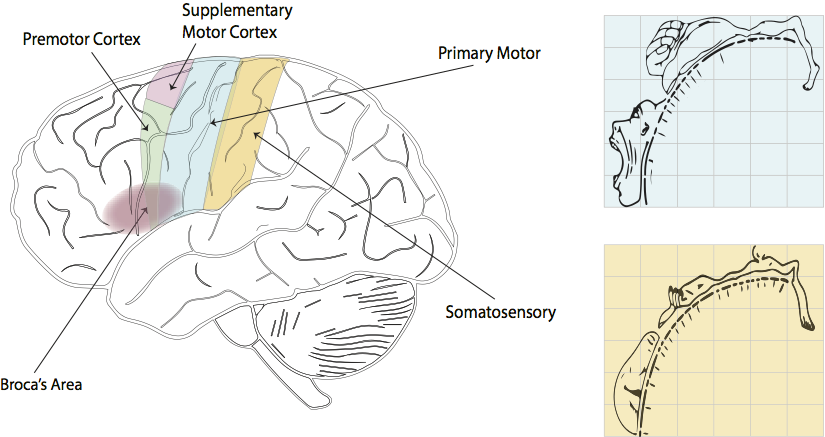
\includegraphics[scale=.8]{./images/brain_motor.png}
\caption[Pamela Payne.]{Somato-sensory and motor processing.}
\label{brain_motor}
\end{figure}
% Add "cortex" to somatosensory label and rearrange labels a bit

\subsection{The Frontal Lobe}
 
 % Cohere with what Chelsea says: ventro-medial planning, orbito frontal decision making
The \glossary{frontal lobe} is involved in higher-level cognitive functions, or \emph{executive functions}, like the ability to pay attention, select strategies, solve problems, plan actions, make decisions, inhibit or suppress behaviors, and in general control one's behavior. These functional associations rely upon a distributed network of regions including the orbito-frontal, dorso-lateral prefrontal, and ventro-medial areas.\footnote{The \emph{Ventro-medial prefrontal cortex} has been shown to be involved in the representation of the internal state of the body and the relative value of decisions. \emph{Orbito-frontal cortex} is also involved in decision-making and is thought to play a particular role in assessing reward.} The rear-most parts of the frontal lobe, like the \glossary{primary motor cortex}, are directly involved in action. In fact, the frontal lobes can be thought of as controlling action on a spectrum from specific movement in the primary motor cortex to  increasingly abstract planning and decision making in the front-most parts of the cortex, like the orbito-frontal cortex. Some language processing also takes place in the frontal lobe. \glossary{Broca's area} (Fig. \ref{brain_motor}) is responsible for many language functions, including gesture, understanding of action and action-language, and language production. 

\begin{figure}[h]
\centering
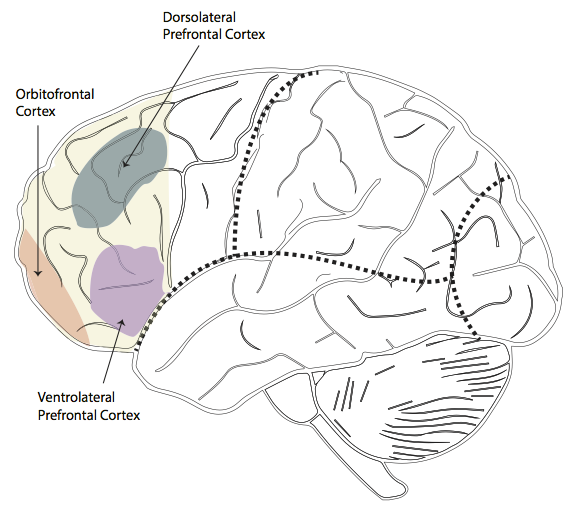
\includegraphics[scale=.75]{./images/brain_frontal.png}
\caption[Pamela Payne.]{The prefrontal cortex.}
\label{brain_frontal}
\end{figure}
% Change the VLPFC to VMPFC in picture and in label.

The parts of the frontal lobe closer to the center of the brain are directly involved in controlling the body. Neural outputs to the body originate in the \glossary{primary motor cortex} (see Fig. \ref{brain_motor}). When parts of the primary motor cortex are stimulated people contract the relevant muscles of their body. When \emph{premotor cortex} is stimulated, people will actually start to make complex movements, such as grasping. \emph{Supplementary motor cortex} is less well understood and does not include a map of the body in humans, but this region is thought to play an important role in coordinating movement plans, in particular sequences of movements.

The dorso-lateral \glossary{prefrontal cortex} or PFC is associated with working or short-term memory. It is part of the cortex but has evolved a distinctive structure that supports the unique demands of working memory. Its cells are relatively isolated from other areas, but with dense recurrent connections that facilitate a particular type of neural dynamics, an ``attractor structure'' (see chapter \extref{ch_dst}), whereby activations tends to settle into stable patterns for a time, which are maintained in cortical ``stripes'' \cite{kriete2013indirection}. These stripes are thought to encode task information in working memory. Your current plans and goals are maintained by active stripes in your PFC. As you go through your day doing one thing after another--making breakfast, driving to school, reading a book, etc.--different stripes corresponding to current goals are sequentially activated in PFC. Support for this idea is provided by experiments that show that while humans and monkeys maintain goals to look or reach in different directions, specific populations of neurons are active in the PFC. In some neural network models, actively maintained tasks are simulated simply by clamping certain nodes in the on or off position. For example, one node might correspond to reading letters, while another might correspond to saying what color the letters are written in, in a model of a task where you can either read letters or say their color.\footnote{These are models of the Stroop effect; see \url{https://en.wikipedia.org/wiki/Stroop_effect}}
% Add Simbrain Stroop network reference
% Add the reference to the empirical literature

% Citations needed
% Primary motor regions process simple movement, while premotor regions are involved in complex goal-based movement, while further forward information about higher goals is integrated. 
% Broca's aphasia isn't  mentioned...
% Give examples of broca's and wernickes aphasia?  E.g. from wiki example of broca's or expressive aphasia speech:  "Yes... ah... Monday... er... Dad and Peter H... (his own name), and Dad.... er... hospital... and ah... Wednesday... Wednesday, nine o'clock... and oh... Thursday... ten o'clock, ah doctors... two... an' doctors... and er... teeth... yah.[10]"

 Damage to the frontal lobe results in a variety of deficits, including difficulties with impulse control, impaired judgment, personality abnormalities, and an inability to make any decisions at all. A famous case of damage to the frontal lobe is provided by Phineas Gage, a 19th century railroad worker whose skull was pierced by a large iron rod in an explosion. Once the iron rod was removed, Gage retained full cognitive function, and the only prominent change was in his behavior. After the surgery, he had a more difficult time inhibiting certain behaviors, became more hostile, drank excessively, and eventually became homeless.

\subsection{Other Neural Networks in the Brain }

We have been focusing on the cortex, which is by far the most dominant structure in the brain. Many neural network models are basically modeling cortex and how it extracts features from sensory inputs layer by layer, maintains task information in the frontal areas, etc. These are models of different aspects of long-term memory. However, there are also many other specialized circuits that have been modeled by distinctive forms of neural network model. See figure \ref{brain_internal} for an overview of the structures we discuss here.

\begin{figure}[h]
\centering
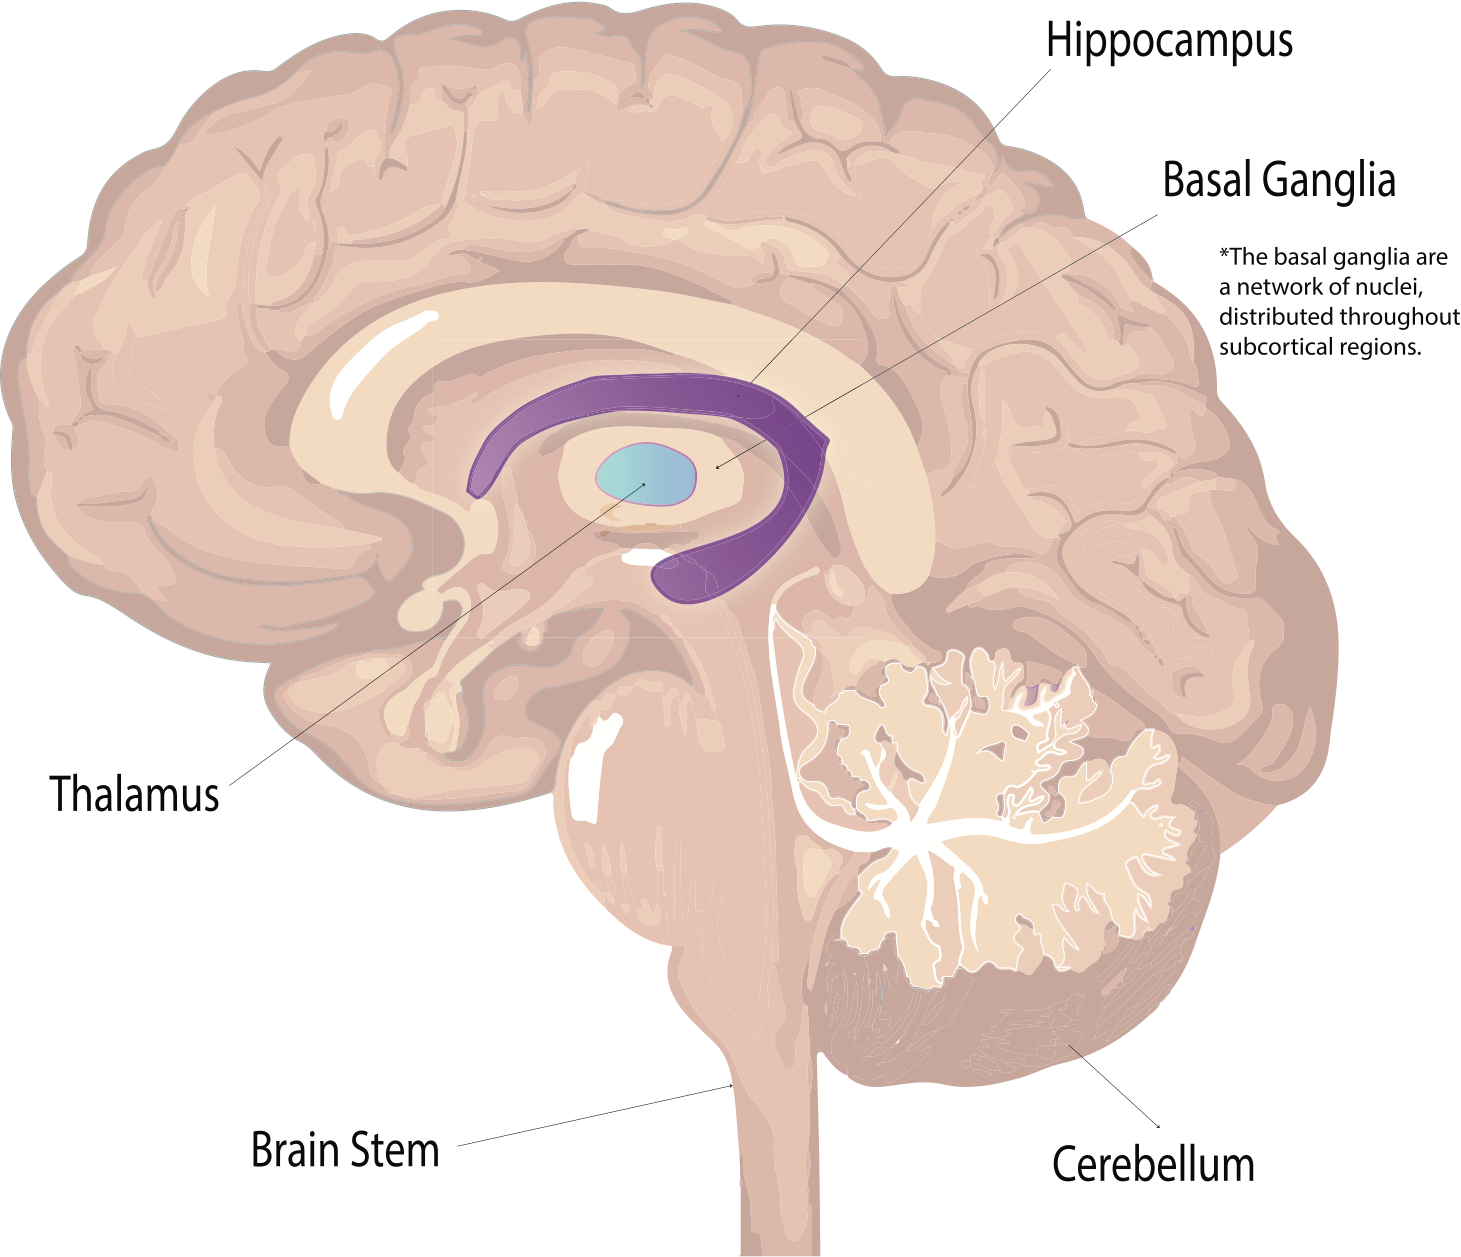
\includegraphics[width=.5\textwidth]{./images/brain_internal.png}
\caption[Pamela Payne.]{Some specific structures in the brain with specific neural network structures.}
\label{brain_internal}
\end{figure}

% Below should add retrograde amnesia and explain the difference
% Episodic memories more in hippocampus
The \glossary{hippocampus} is a kind of short-to-medium-term memory system attached to the bottom of the cortex.\footnote{In fact it is directly attached to the temporal lobes, and is hard to see as being separate on visual inspection, but its neurons are arranged differently than the neurons in the cortex.} It is associated with memory consolidation, spatial memory, and episodic memory. It has a special neural network structure that allows it to watch what is happening in the cortex, and then build up special ``sparse coded'' representations.\footnote{For simulation-based tutorials on computational models of hippocampus see \url{https://compcogneuro.org/}.}  While learning in the cortex is slow, learning in the hippocampus is fast. It can pick up all the things that happen in your day and remember them for a few weeks or even longer. These memories don't always last, and in fact new neurons are constantly being created in hippocampus (it's one of the few parts of the brain where neurogenesis continues into adulthood). Dreams are thought to be mediated by hippocampus, which is why dreaming often involves recent events. When things get repeated enough in hippocampus, they are consolidated into the cortex. It's like it learns a fast representation, and then that either evaporates or if repeated enough, gets transferred to cortex. Damage to the hippocampus can produce various forms of amnesia, e.g. \glossary{anterograde amnesia}, now familiar via movies like \emph{Memento}, where characters live entirely in the present and cannot remember things that they learn after the date of their injury. Interestingly, patients with this form of amnesia are often able to create new \emph{procedural memories}, such as a ``memory'' of how to ride a bike, but are unable to create any new episodic, semantic, or fact-based memories, such as memories of events in the news. Neural network models of hippocampus have been used to study how memories can be consolidated into long term memory. The models can, for example, be used to simulate amnesia.
% Also spatial maps of the environment
% Citations

 The \glossary{basal ganglia} is an important collection of nuclei beneath the cortex which have a variety of functions, including (in concert with pre-frontal cortex) control of voluntary action, and learning how to take actions that are likely to lead an agent to rewarding stimuli. It is thought to implement a form of \glossary{reinforcement learning}, whereby actions that produce reward tend to be reinforced over time, and actions that produce costly outcomes are inhibited (this formalizes older ideas in psychology about operant conditioning). It's a bit like a task scheduler or sequencer, orchestrating extended sequences of activations in the cortex. It is also thought to be involved in deciding what tasks and goals should be loaded into the frontal areas of the brain, determining what tasks are maintained in PFC's stripes, and in what sequence. It implements reinforcement learning in part using the neuromodulator dopamine, discussed above. These same reinforcement learning techniques have also been shown to work well in machine learning.\footnote{Reinforcement learning was, for example, used in Alpha Go (mentioned in chapter \extref{ch_intro}), the first neural network to beat a professional human Go player \url{https://deepmind.com/research/alphago/}} In fact, there was a great deal of excitement in the 1990s when it was first discovered that dopamine neurons in the basal ganglia responded to rewards in the same way as certain variables in reinforcement learning models: more activity when reward is higher than expected; less activity when reward is less than expected  \cite{schultz1997neural, niv2009reinforcement}.  When things go better than we expect, dopamine is released, and synapses are strengthened, reinforcing whatever we have done recently, making us more likely to do the same thing in the same situation in the future. Thus the dopamine system and the basal ganglia ``sequencer'' learns to execute sequences of goals and actions that tend to produce reward in the long run and avoid punishment.\footnote{Some of these ideas can be studied using the actor-critic model in Simbrain (available from the simulation menu). Links to operant conditioning can be studied using the Rescorla-Wagner and operant conditioning simulations).  The relation to frontal lobes and task maintenance is explored in CECN models at \url{https://compcogneuro.org/}.}
% Glossary for  dopamine, mid-brain?
% More citations
 
\begin{figure}[h]
\centering
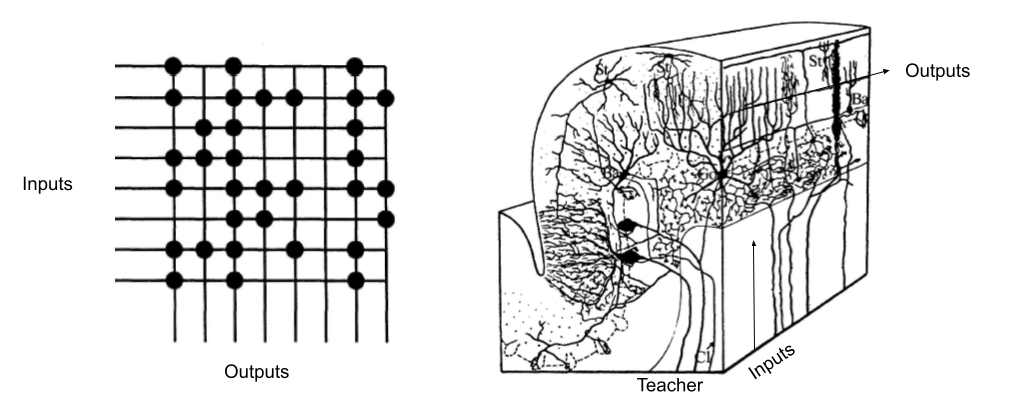
\includegraphics[scale=.3]{./images/cerebellum_Associator.png}
\caption[From lecture slides by David Touretsky.]{The cerebellum as a pattern associator, mapping sensory states to motor actions. (Left) An input-output architecture: synapses where input lines and output lines overlap can be turned on when a teacher signal turns on. (Right) Associated areas of the cerebellum thought to correspond to these functions.}
\label{cerebellum_associator}
\end{figure}
% Get original figure attributions and add citation.
% Add arrows to the figure!

The \glossary{cerebellum} is involved in fine motor control (it also has cognitive functions but these are less well understood). When it is damaged, movement becomes jerky and ballistic (\glossary{ataxia}). Neural network models treat the cerebellum as a massive pattern associator, or even as a neural ``lookup table''. It has a structure that made it an attractive target for computational neuroscientists in the late 1960s and early 1970s \cite{marr1991theory}. As can be seen in figure \ref{cerebellum_associator}, it receives many inputs and produces many outputs, and there are also neurons that seem to climb up and surround certain neurons, suggesting that they carry an error signal used to update certain synapses. This led to the idea that it was a pattern associator trained by supervised learning, a theory which remains popular, though the issue is not settled. One thing it certainly does is learn to associate bodily and sensory inputs with motor outputs, which helps produce rapid and smooth action sequences. It's as if the coarse-grained motor plans produced by the cortex and basal ganglia are ``smoothed'' by this cerebellar associative map.

The \glossary{thalamus} is a subcortical region responsible for  processing and relaying information between the cortex and  sensory and motor structures on the body. Information from most  sensory modalities passes through the thalamus on the way to the cortex. It is sometimes called the ``gateway to the cerebral cortex.''  Recurrent loops between the thalamus and cortex (\emph{thalamo-cortical loops}) produce wide-spread synchronized patterns of activity in the cerebral cortex which are, as noted above, associated with conscious experience.

Finally, more fundamental functions of the brain, like the control of the lungs, heart, and sleep, take place in the \glossary{brain stem}. Damage to the brain-stem often results in death.
% Draw on Solms and Damasio. Homeostasis. Also how we can be cs without cortex but still be situationally and affectively responsive.


%\chapter{Activation Functions}\label{ch_act_functions}
\chapterauthor{Jeff Yoshimi, Scott Hotton}

 As discussed in the introduction, artificial neural networks are comprised of nodes connected by weights. The nodes are usually pictured as  circles, and are associated with a number called an activation, while the weights are represented by lines connecting the nodes, and are associated with a number called a strength. In Simbrain node activations correspond to the colors of the nodes and the number inside the nodes, and weight strengths correspond to the color and size of the filled disks at the end of the lines connecting nodes. In figure \ref{F:simplenet1} (Left), three nodes are connected to one node via three weights. 

When a neural network simulation is run, node activations and weight strengths change. Neural networks have \emph{dynamics}, which describe a changing pattern of activation across the nodes and (in some cases) a changing pattern of strengths of across the weights. To see these dynamics in Simbrain, look for the triangular ``play''  button 
\includegraphics[scale=.5]{./images/Play.png}. When you press it you usually see node activations change and in some cases weight strengths.In this chapter we describe some of the rules that govern changing node activations.\footnote{When you open up a dialog to train a network, there is another play button that is used to modify the weights. When these buttons are pressed the dynamics of nodes and weights is simulated. In chapters \extref{ch_linear_algebra}, \extref{ch_unsupervised}, and \extref{ch_supervised} we discuss the rules governing changes in weight strengths.} These are based loosely on the physiology of neurons and action potentials, which was discussed in chapter \extref{ch_neuro}. 

Rules for updating node activations make use of an \glossary{activation function}, which sets the activation of a node based on the values of incoming node activations and the weights connecting them together. These are classical rules that have been used in many kinds of simulations since the early days of neural networks. There are many other rules for updating neural networks--some geared more towards computational neuroscience, some towards engineering--but even today these classical rules are frequently used.\footnote{To get a sense of the diversity of functions available, try editing a few nodes in Simbrain (double clicking on them) and changing the 
``update rule" drop down box. As you change the selection you will notice that 
the parameters available to you change. You can also wire together a small 
network and just see what happens when you use these rules. Several neurally realistic ``spiking'' activation rules are included in Simbrain, which are discussed further in chapter \extref{ch_spiking}.}

\begin{figure}[h]
\centering
\raisebox{-0.5\height}{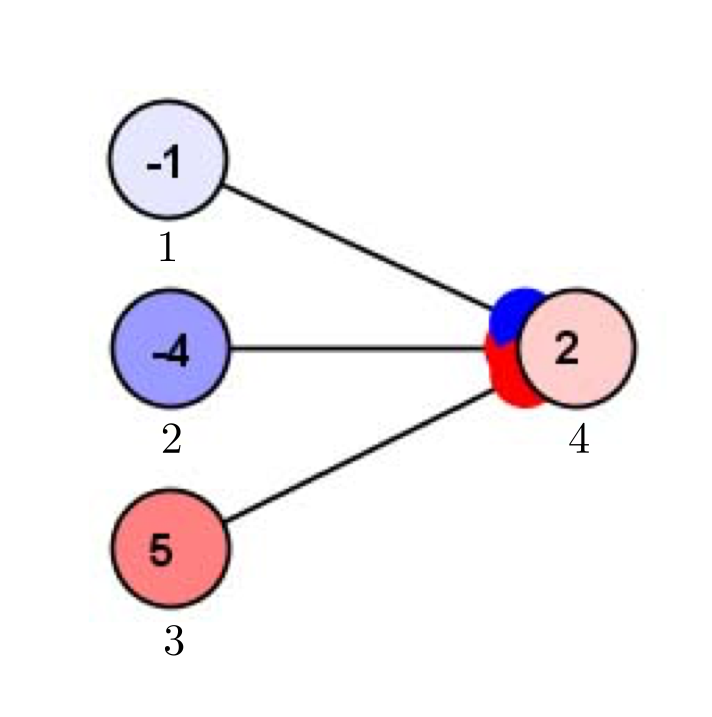
\includegraphics[scale=.7]{./images/Simple3Labelled.png}}
\hspace*{.4in}
\raisebox{-0.5\height}{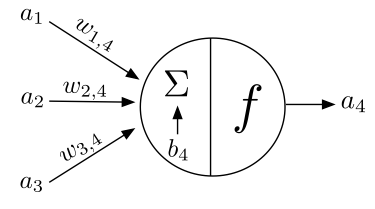
\includegraphics[scale=.7]{./images/activationFunction.png}}
\caption[Left: Simbrain screenshot; Right: Jeff Yoshimi.]{(Left) A simple neural network, with three nodes attached to one node via three weights. (Right) Schematic of the same network to illustrate the notation being used here. Nodes $1,2, 3$ are connected to node $4$. In this example, $a_1 = -1$, $a_2 = -4$, $a_3=5$ and (though weight strengths are not visible) $w_{1,4} = -1$, $w_{2,4} = 1$, $w_{3,4} = 1$, $b_4 = 0$ and the activation function is linear with a slope of 1, so that $a_4 = 2$. $\Sigma$ represents the weighted inputs, and $f$ represents the activation function. A network like this is included with Simbrain as \emph{simpleNet.zip}}
\label{F:simplenet1}
\end{figure}
% Add x-y axis lines? 

\section{Weighted Inputs and Activation Functions}

 We will represent the activation of the $j^{\rm th}$ node of a network by $a_j$. The 
strength of the weight connecting the $j^{\rm th}$ node to the $k^{\rm th}$  node will be denoted by $w_{j,k}$. This notation is illustrated in figure \ref{F:simplenet1}. Activation $a_j$ of node $j$ is updated by first 
computing the weighted input to node $j$  (roughly: the weighted sum of activations from other incoming nodes) and then passing that value through an activation function denoted by $f$. The basic flow of operations is shown in figure \ref{F:simplenet1} (Right). In this section we discuss weighted inputs in more detail, and then consider three of the most common forms for the activation function: threshold, 
linear, and sigmoid.
% The notation w_j,k is not always followed. Sometimes the opposite is used, where i is target and k is source. (ex. Matlab neural net docs). Faussett has a nice way of putting it.
% This is called a ``local field'' or ``activation potential'' by Haykin

\begin{figure}[h]
\centering
\includegraphics[scale=0.130]{./images/graph_binary4.pdf}
\caption[Scott Hotton.]{The graphs for three activation functions. In each of the graphs the 
horizontal axis is the weighted input, $n_k$, and the vertical axis is the 
activation, $a_k$. Left: A threshold activation function with $(u,\ell,\theta)
=(1,0,0.5)$. Middle: A piecewise linear activation function with 
$(u,\ell)=(1,0)$. Right: A sigmoid activation function with $(u,\ell,m) = 
(1,0,1)$. The inflection point is located where the horizontal dotted line 
$a_k = (u+\ell)/2$ intersects the vertical axis. The tangent line to the graph 
at the inflection is shown by the dotted line with a slope of $1$. The graph 
converges to $1$ as the weighted input increases and to $0$ as it decreases.}
\label{activationFunctions}
\end{figure}

% Discuss relation to gain, relate to excitability. 

A basic feature of a node's activation is that it is a function of the activations of other nodes attached to it, and also the strengths of the intervening weights. This can be computed as a simple linear combination of incoming activations to a node, and intervening weights, which is called the  \glossary{weighted input} (or ``net input'') to a node. That is, each incoming activation to a node is multiplied by the intervening weight strength, and these products are added together. We denote the weighted input to the $k^{\rm th}$ node as ``$n_k$''. 

Nodes are also associated with a \glossary{bias}, which is a fixed and unweighted input to a node (it can also be treated as an input via a fixed weight whose strength is 1). It can be thought of as a property of the node itself (in Simbrain it is set by editing a node's properties), that determines the node's baseline level of activity.

The value of the weighted inputs $n_k$ to a node is computed by multiplying the activations of incoming 
source nodes $a_j$ by the intervening weights $w_{j,k}$, and adding any bias $b_k$.
In the example shown in figure \ref{F:simplenet1},  $n_4$ can be expressed as:
\begin{eqnarray*}
n_4 = \sum_{j=1}^{3} (a_j w_{j,4})  + b_4 = (a_1 w_{1,4})  + (a_2 w_{2,4}) + 
(a_3 w_{3,4}) + b_4
\end{eqnarray*}
If we have $N$ inputs, then the value 
of $n_k$ can be concisely expressed as:
\begin{eqnarray*}
n_k = \sum_{j=1}^{N} a_j w_{j,k}  + b_k
\end{eqnarray*}
If you are not familiar with the symbol ``$\sum$'', it is described in this footnote.\footnote{We use ``sigma'' notation to represent the 
addition of several numbers. Sigma is the name of the Greek letter for 's' 
which is short for 'sum'. The letter has uppercase and lowercase forms. The 
uppercase sigma is used to denote summation. For instance the sum of the cubes 
of the first $4$ positive integers can be written as 
$\displaystyle{\sum_{j=1}^{4} j^3 = 1^3 + 2^3 + 3^3 + 4^3 = 1 + 8 + 27 + 64 = 
100}$. The uppercase Greek letter `$\Sigma$' tells us that we are to perform a 
summation. Beneath $\Sigma$ it says `$j=1$'. This tells us that we are going 
to increment $j$ starting with the value of $1$. Above $\Sigma$ it says `4' 
which tells us to stop incrementing $j$ at the value $4$. The $j^3$ to the 
right of $\Sigma$ tells us to cube each of the values for $j$. We start of 
with $j=1$ and cube it. Next increment $j$ and cube that and continue until 
$j=4$. Finally we sum all four of the cube numbers we got. Often we use a 
letter for the final value of the incremented variable so that our formulas 
will work with sums with an arbitrary number of terms. For instance 
$\displaystyle{\qquad \qquad \sum_{j=1}^{N} i^3 = 
\left(\frac{N(N+1)}{2}\right)^2}$.}

Some examples of computations of weighted input are provided below.

We now consider the activation function (labeled by `$f$' in figure
\ref{F:simplenet1}), which associates weighted inputs with activation 
values. Activation functions are sometimes also called ``transfer functions''. Recall 
that in mathematics, a function $f$ associates a unique output to each input. 
We say the input is mapped to the output. For example if $f(x) = x^2$ 
then  
\begin{eqnarray*}
{\rm The\; input\; 1\; is\; mapped\; to\; the\; output\; 1}.
\qquad f\colon 1 \mapsto 1 
\qquad f(1)=1^2 = 1 \\ 
{\rm The\; input\; 2\; is\; mapped\; to\; the\; output\; 4}.
\qquad f\colon 2 \mapsto 4
\qquad f(2)=2^2 = 4 \\
{\rm The\; input\; 3\; is\; mapped\; to\; the\; output\; 9}.
\qquad f\colon 3 \mapsto 9
\qquad f(3)=3^2 = 9 
\end{eqnarray*}

   Two parameter values will be used repeatedly in this section: an upper value 
$u$, and a lower value $\ell$ (of course, we assume $\ell < u$). In Simbrain, the upper and lower values $u$ and 
$\ell$ are set in the \emph{upper bound} and \emph{lower bound} fields of a neuron, respectively.\footnote{Except in the case of the binary threshold neuron, where the $u$ is an ``on value'' and $\ell$ is an ``off value.''  These values are sometimes also referred to as ``ceiling'' and ``floor''.}  It will sometimes be useful to refer to these parameter values using vector notation. For example a statement like $(u,\ell) = (1,-1)$ means that $u = 1$ and $\ell = -1$. 

\section{Threshold Activation Functions}

%"hard limiter"?
   We begin with a simple activation function, the \glossary{threshold
activation function} (it is also called a ``binary'' activation function, a ``step function'', or a 
``Heaviside function'').\footnote{The term ``binary'' refers to the fact that the
node can only take on one of two values. The term ``step function'' refers to the way the function appears when plotted (see figure \ref{activationFunctions}). The term ``Heaviside'' is a reference to Oliver Heaviside  who used these functions to study electrical circuits.}  These nodes can take on one of two values, an upper 
value $u$ and a lower value $\ell$, and they are thus binary valued nodes. 
Which value the node takes on depends on whether weighted input is greater than 
or less than a threshold value $\theta$. Threshold 
activation functions are inspired by real neurons, which operate in a 
discrete, on-off fashion, either firing or not firing an action potential
depending on a summation of incoming excitatory and inhibitory currents (see section \extref{simpleNeuralDynamics}).

   If the value of the weighted input to a threshold activation function is less 
than or equal to a threshold value $\theta$ then the activation of a threshold 
node takes on a lower value $\ell$. If the value of the weighted input is greater 
than $\theta$ then the activation of a threshold node takes on an upper value 
$u$.
\begin{eqnarray*}
    a_k = f(n_k) =  \left\{
        \begin{array}{lc}
        \ell & {\rm if} \; n_k \leq \theta \\
        u  & {\rm if} \;  n_k >  \theta
    \end{array} 
    \right.
\end{eqnarray*}
The graph of a  threshold activation function is shown in figure \ref{activationFunctions}. When the 
weighted input increases from below the threshold of $0.5$ to above the threshold 
the function's output jumps from the lower bound, $0$, to the upper bound, 
$1$.

%For the special case where $u = 1$, $\ell = -1$, and $\theta = 0$, the function can (almost) be written using a sign or signum function: $a_k=\mbox{sign}(n_k)$. That is, the activation of the node is equal to the sign of its weighted input. If weighted is positive, the activation is 1, if it's negative, it's -1. However if the weighted inputs are 0, the activation is 0, producing a third possible output.

% Note that the bias term can effectively translate the graph of the piecewise linear function left or right
% See Haykin's discussion. It's an affine transform.

\section{Linear Activation Functions}\label{S:linearact}

 A \glossary{linear activation function} computes activation as a simple linear function 
of weighted input. To compute the activation we simply multiply the weighted input 
by the positive number, $m$. This number is the slope of the linear function.
\begin{eqnarray*}
a_k = f(n_k) = m  \cdot n_k
\end{eqnarray*}
$m$ is usually set to 1 so that a linear activation function is the identity function (which takes every input to itself). This means that the activation of a node when it uses a linear activation with $m = 1$ just is the weighted inputs to the node.

A related type of activation function is a \emph{piecewise linear} function. (For this discussion we assume that $m=1$). For a piecewise linear function if the  value of the weighted input is less than $\ell$ then the activation is set to the lower value $\ell$. If the value of weighted input is greater than $u$ then the  activation is set to the upper value $u$. For values between the upper and lower bound the activation is the weighted input:
\begin{eqnarray*}
a_k = f(n_k) =  
\left\{
      \begin{array}{clc}
                  \ell      & {\rm if} &   n_k\; < \; \ell             \\
              n_k  & {\rm if} &  \ell \;\leq\; n_k \;\leq\; u \\
               u     & {\rm if} &    n_k > u
      \end{array} 
\right.
\end{eqnarray*}

A piecewise linear function is basically a clipped or truncated linear function. As the weighted inputs to a node get very large or small, the activation is truncated to the upper or lower value. This is biologically realistic (a membrane potential can't achieve arbitrarily high or low values; a neuron can't fire at arbitrarily high rates). Also, it is not uncommon for a neural network algorithm to produce uncontrolled growth or decay, which can be prevented by the simple act of truncating the signal for certain values.\footnote{In Simbrain, nodes are piecewise linear with $m=1$ by default, so that by default a node simply displays weighted inputs, assuming weighted inputs fall within the upper and lower bounds of the neuron. A linear node can be converted in to a regular, non-piecewise linear node by turning off  \emph{clipping}.}

\begin{figure}[h]
\centering
\includegraphics[scale=.4]{./images/relu.png}
\caption[Scott Hotton.]{Graph for the rectified linear or ``relu'' activation function.}
\label{relu}
\end{figure}
% Redo figure

A special case of a piecewise linear activation function is a \emph{rectified linear unit} or \glossary{relu activation function}. The terminology comes from electronics where rectifiers are often used to truncate the negative part of an alternating current to produce a direct current. They cut off all negative values, replacing them with a 0, and leave the weighted input unchanged otherwise (see figure \ref{relu}).\footnote{The rule can be more concisely stated as the maximum value between 0 and $n_k$, or $\mbox{max}(0,n_k)$.} Thus they are a piecewise linear function with no upper bound:
\begin{eqnarray*}
a_k = f(n_k) =  
\left\{
      \begin{array}{clc}
                  0      & {\rm if} &   n_k\; <= \; 0          \\  
              n_k  &  &  \mbox{otherwise}	
      \end{array} 
\right.
\end{eqnarray*}
This can be useful because it removes all negative activations, making overall activation in a large network more sparse. The function also has a simple derivative\footnote{0 or the slope, except at the point of discontinuity, where the derivative is not defined.}, and other mathematical properties which have made it extremely popular, especially for deep networks, so much so that there are now multiple varieties of special relu functions available, like ``gelu''. In Simbrain a relu unit can be approximated by setting a linear neuron to linear, and setting \emph{lower bound} to 0 and \emph{upper bound} to a large number.

\section{Sigmoid Activation Functions}

% Reference to sigmoid's use in Stroop model (see 2009 section on "AttentionStroop")
% Also see "ossification" in Elman ``starting small'' paper

A \glossary{sigmoid activation function} can be thought of as a smoothed version of a piecewise linear activation function. The sigmoid functions get their name from the Greek letter for ``s'', and their graphs are sometimes called ``s-curves'' because they resemble a stretched-out letter ``s''. This is directly visible in figure \ref{activationFunctions}. As weighted inputs increase the activation approaches the upper value $u$, which is usually 1. As weighted inputs decrease the activation approaches the lower value $\ell$, which is usually 0 or -1. When weighted inputs are near the inflection point of the function at 0, activation changes rapidly. Since outputs are always ``squeezed'' between $u$ and $l$ it is sometimes called a ``squashing function.''

  Sigmoid  functions can be used to describe many natural processes which increase continuously from one value to another, such as fruit size, population growth, or  neural activity. Suppose a bacterium is placed in a Petri dish and we observe how quickly bacteria grow in the dish. At first the population grows slowly. Then it is rapidly expanding in a neighborhood of the inflection point. Then as the population begins to fill the dish the population size levels off or plateaus. Something similar happens when to the firing rate of a neuron as it receives more input currents. At first the firing rate rises slowly, then rapidly, and then it approaches a maximum value.
 % Add more details and references?  Put a bacterium in a petri dish. Close to low value, far from high value. Not much in first hour. Doubling time of 5 minutes. Dividing every 10 minutes. Early stage corresponds to exponential growth. After inflection point exponential decay. // Scott chose  fruit example because the curves are _really_ well modeled by Sigmoid. The bacteria case is more famous but has a bit of noise in there once the dish gets filled up.

Sigmoid activation functions are notable for being differentiable everywhere. If you have not taken calculus, this intuitively means that the function smoothly changes everywhere; there are no discontinuous breaks or hard edges. Notice that the threshold and piecewise linear activation functions in figure \ref{activationFunctions} are not differentiable everywhere. The threshold function has a discontinuity at the threshold value and the piecewise linear function does not change smoothly at the truncation points $(u,u)$ and $(\ell,\ell)$. The relu function is discontinuous at $(0,0)$. The differentiability of the function means that the derivative can be used, which in turn allows certain operations to be performed on sigmoidal nodes that would not otherwise be possible. This led to one of the major innovations in the history of neural networks; the move from linear networks (networks of nodes using linear activation functions) to networks using sigmoidal nodes, which could be trained using backpropagation. This led to an increase in the use of neural networks in the 1980s (see chapter \extref{ch_history}). 

   We will not focus on how to compute a sigmoid function here (the function can be computed in several different ways). We focus on 
the qualitative properties of sigmoid functions. However, to give a flavor of 
the idea, here is one common way by which some sigmoid functions can be 
computed: 
\begin{eqnarray*}
a_k = f(n_k) = \frac{1}{1+e^{-4\, m\, n_k}}
\end{eqnarray*}
(Note that this version of the function incorporates a slope parameter $m$ but not an adjustable upper or lower value. Adding $u$ and $\ell$ parameters would make the function even more complex). This version of the sigmoid function is often called a ``logistic function.''  There are other versions of the sigmoid function, for example, one based on the arctangent function from trigonometry, and another based on the hyperbolic tangent function.\footnote{In Simbrain this function is captured by the ``Sigmoidal (Discrete)'' update rule. Different implementations of the function can be selected within Simbrain.} 
% The 4 is there so that the derivative ends up being m
% logit function.... inverse of logistic?  Shows in logistic regression. All that stuff with link functions and generalized linear model might be worth mentioning here.

In general we need three values to specify a particular sigmoid function. We 
need its upper bound, $u$, its lower bound, $\ell$, and a positive slope $m$. 
For the formula above $(u,\ell) = (1,0)$ and $m$ can have any positive value.
   When the weighted input to a sigmoidal function equals $0$, the resulting activation will be exactly half way 
between the upper and lower bounds, \ie $(u + \ell)/2$, or in this case $(1+0)/2 = .5$. 
The point $(0,  (u + \ell)/2)$ on the graph of the sigmoid function is called the {\em 
inflection point} of the function. Each sigmoid function is symmetrical about
its inflection point. The value of $m$ is the slope of the tangent line to the 
graph of the sigmoid function at the inflection point. In other words $m$ 
tells us how steeply the graph of a sigmoid function rises.

   As the weighted input is increased indefinitely above $0$ the value of a 
sigmoid function converges to its upper bound $u$. As the weighted input is 
decreased indefinitely below $0$ its value converges to its lower bound $\ell$.
The larger $m$ is the more rapidly the sigmoid function converges to its 
bounds. figure \ref{activationFunctions} shows the graph of a sigmoid function with 
$(u,\ell,m) = (1,0,1)$. 

As the slope parameter is varied, the shape of the sigmoid function changes. When the slope is
large or ``steep'', the sigmoid will begin to look like the threshold function. When the slope is near 0, it will begin to look more like a linear function.
% \chapter{Linear Algebra and Neural Networks}\label{ch_linear_algebra}
\chapterauthor{Jeff Yoshimi, Scott Hotton}

% Also see "indexing hell" comment at  http://neuralnetworksanddeeplearning.com/chap2.html

% Identity matrix

% NN discovers faster matrix product: https://www.nature.com/articles/s41586-022-05172-4. Oddly meta.

In this chapter, we review some basic concepts of linear algebra with an 
emphasis on how they can be applied to the study of neural networks. This can be viewed as a transition from the formal structure of single nodes and weights, to the formal structure of \emph{lists} and \emph{tables} of nodes and weights. In particular, we  consider vectors and matrices, which allow us to describe the behavior of groups of nodes and weights in a compact way.

Linear algebra also facilitates a powerful geometric framework for \emph{visualizing} the structure and dynamics of a neural network. The properties of a set of inputs and whether they can be properly classified is an example of something that is  more intuitively understandable when the input vectors are visualized as points in a space. Chapter \extref{ch_act_functions} notes that whenever the ``play''  button \includegraphics[scale=.5]{./images/Play.png} is pressed in Simbrain, some dynamical process is simulated. The framework of linear algebra makes it possible to visualize the changing activations of a set of nodes, or the changing strengths of a set of weights, as a moving point in a space. This approach to thinking about neural networks uses \emph{dynamical systems theory}, discussed in chapter \extref{ch_dst}, and can be used to think about many features of neural network models in an intuitive way.\footnote{For a quick demonstration of this way of visualizing network dynamics, try running the simulation \emph{highDimensionalProjection.bsh}. The dynamics of the network is visible in the projection component.}  

\section{Vectors and Vector Spaces}\label{sect_vector}

% This needs to be done in an intuitive way first, then formalized
    Linear algebra is the study of vector spaces. Vector spaces are abstract
mathematical systems that turn out to be extremely useful for describing the 
structure and dynamics of neural networks. A \glossary{vector space} is a 
collection of objects called \glossary{vectors} along with mathematical 
operations that we can perform with the vectors.\footnote{You may have heard 
that vectors are geometric objects that have a magnitude and a direction. You 
may have seen them represented by an arrow or directed line segment. These 
different points of view on vectors supplement rather than contradict each 
other.}  For instance, we can add two vectors together to get another vector. There is also a type of 
multiplication that can be performed between a vector and a \glossary{scalar}. The term ``scalar'' is used for those numbers that are allowed to be 
multiplied with a vector. We will focus on the case where scalars are real numbers, like $2$, $-1.2$, or $5.9$. If the scalars are the set of real numbers, then the 
vector space is called a {\em real vector space}. We will only work with real
vector spaces. A more formal definition for a vector space is discussed in 
Sect. \ref{S:LinearAlgebraAppendix}. 

We will represent vectors as ordered lists of scalars.\footnote{ Many classes of mathematical objects satisfy the formal definition
of a vector space, and thus many objects can be vectors. The ordered lists we consider here are an especially convenient type of vector.} Each of the scalars in the list is called a \glossary{component} 
of the vector. A list with 2 components is called an {\em ordered pair}. A 
list with 3 components is called an {\em ordered triple}. More generally, a
list with $n$ components is called an {\em $n$-tuple}. We can refer to the
members of a vector in this sense  as its ``first component'',  ``second component'', etc.
A vector in the sense of an $n$-tuple is often 
written out as a comma-separated list of numbers surrounded by parenthesis. 
For example, here are four vectors:
\begin{equation*}
    (0,0) \quad (0,1) \quad (1,0) \quad (1,1) 
\end{equation*}

% TODO: Expand this as we use this more and decide if any convention regarding indices should be given now.
   We sometimes adopt the convention of writing vectors using bold-faced 
lower-case letters, for example $\mathbf{a}_i$ for a  vector of input values, 
$\mathbf{t}$ for a vector of target values, or $\mathbf{a}_4$ for the 
activation vector in the fourth node-layer of a feed-forward network.  By 
contrast non bold-faced, italic lower-case letters are usually reserved for 
components of vectors, and the subscript indicates which component. For 
example, $a_2$ could designate the second component of an activation vector 
$\mathbf{a}$.

When the components of a vector are written horizontally, from left to right,
it is called a {\em row vector}. The ordered pairs shown above are row 
vectors. The components can also be written out vertically, from top to 
bottom, in which case the vector is called a {\em column vector}.\footnote{The choice of whether
to use a row or a column vector to represent an abstract vector is primarily a matter of 
convenience or convention.} Commas are usually 
not written in column vectors because it is clear what the components are. For 
example, here are four column vectors:
\begin{small}
\begin{equation*}
\begin{pmatrix}
0 \\
0
\end{pmatrix} 
\quad 
\begin{pmatrix}
0 \\
1
\end{pmatrix} 
\quad 
\begin{pmatrix}
1 \\
0
\end{pmatrix} 
\quad 
\begin{pmatrix}
1 \\
1
\end{pmatrix} 
\end{equation*}
\end{small}
The number of components in a vector can be any positive integer. If there is
only one component, then the vector is essentially just a scalar.

   For any positive integer $n$, the set of all $n$-tuples forms a vector space.
The integer $n$ is called the \glossary{dimension of a vector space}. For 
example, the set of all of ordered pairs of real numbers is a 2 dimensional 
real vector space $\real^2$. The set of all ordered triples is a 3 dimensional real 
vector space $\real^3$. The set of all possible activations for a network with 172 nodes is a subset of  $\real^{172}$.

   The components of a vector can be thought of as the coordinates of a point
in Euclidean geometry. The components of a vector can be used to locate a
point by starting at the origin and moving parallel to each axis by the 
amount specified by the corresponding component. To locate the point corresponding to the vector 
$(3,4)$, for example, we move $3$ units to the right along the 
horizontal axis and $4$ units upwards along the vertical axis. In this way a 
2 dimensional real vector space can be thought of as an Euclidean plane (see 
figure \ref{2d}).\footnote{There is a legend (probably fabricated, but pedagogically useful nonetheless) 
that the philosopher Ren{\'{e}} Descartes 
 came up with his proof that given a point in the plane there are unique coordinates for that 
 point (and given a pair of coordinates there is a unique point in the plane) 
 while observing flies on his ceiling. He 
 noticed that the position of the flies on the ceiling could be described by 
 superimposing a kind of grid on the ceiling---for example: there's a fly at 
 $(3,4)$, 3 units to the right, and 4 units up; there's a fly at 
 $(-2,-1)$, 2 units to the left, and 1 unit down; and there's another at 
 $(4,-2)$, 4 units to the right, and two units down (see figure \ref{2d}).} 
 
 % This is useful in Simbrain but the connection is a bit lost here 
For 2-dimensional spaces, finding your way around is a bit like using an ``Etch a sketch'' toy\footnote{\url{https://en.wikipedia.org/wiki/Etch_A_Sketch}.}, where you move a tracing point around in a space using one knob for left-and-right ($x$-values) and one knob for up and down ($y$-values). If you plot the activation space of two nodes in Simbrain and adjust the activations of the two nodes, this analogy is useful for understanding what is happening.

\begin{figure}[h]
\centering
\includegraphics[scale=0.175]{./images/grid2.png}
\caption[Scott Hotton.]{Each vector in a 2 dimensional vector space is associated to a point 
in the Euclidean plane by treating the components of the vector as the 
coordinates of the point. Try to find the vectors $(3,4)$, $(-2,-1)$, and 
$(4,-2)$.} 
\label{2d}
\end{figure}

   The number of dimensions of the vector spaces that arise in the study of 
neural networks can be much larger than 3. We we can not geometrically visualize these higher-dimensional spaces directly. To work mathematically in 
these spaces, it is helpful to keep in mind that our starting point is the 
$n$-tuples, which are just lists of numbers. From this standpoint, the 4 
dimensional real vector space we work with is just the set of all $4$-tuples of
real numbers, and the 5 dimensional real vector space we work with is just the 
set of all $5$-tuples of real numbers. Here are some vectors in a 5 
dimensional vector space:
\begin{equation*}
    (0,-1, 1, 0.4, 9)  \qquad
    (-1, 2, 4, -3, 9)  \qquad 
    (0, 0, 0, -1, -1 ) \qquad
    (0, -1, 0, -1, 0 ) 
\end{equation*}
We can keep going. The vectors that make up a 100 dimensional vector space are 
just lists of 100 numbers. The vectors that make up a billion dimensional 
vector space are just lists of a billion numbers. 

   Real vector spaces with more than 3 dimensions cannot be seen directly, but 
objects in them can be \emph{projected} to lower dimensional real vector spaces 
where they can be visualized. We will discuss methods of projection from 
spaces with more than 3 dimensions in Sect. \ref{S:dimReduction}.\footnote{Here
again the Simbrain simulation \emph{highDimensionalProjection.bsh} is helpful.
When you run the simulation, a sequence of points in a 25 dimensional space 
appears. Each point corresponds to a vector. If you hover the cursor over any
one of the points, you will see the list of 25 numbers (the 25 activation levels
for the network) that correspond to that point.}

\section{Vectors and Vector Spaces in Neural Networks}\label{S:dimReduction}

   Vectors are frequently used to describe lists of activations, weights, and other quantities associated with neural networks. 

\begin{figure}[h]
\centering
\raisebox{-0.5\height}{\includegraphics[scale=.5]{./images/ff.png}}
\hspace*{1in}
\raisebox{-0.5\height}{\includegraphics[scale=.3]{./images/recurrent.png}}
\caption[Simbrain screenshots.]{A feed forward and recurrent network in Simbrain. Try to identify the dimensionality of the activation space, input space, hidden unit space, output space, and weight spaces of each network. Left: A feed-forward neural network with activations showing. Right: A 2-node recurrent network with activations showing.}
\label{ffRecurrent}
\end{figure}

% TODO: Run the bold-faced notation through
  The activations of a neural network's $n$ nodes can be described by an \glossary{activation 
vector} with $n$ components, one for each activation value. For example, if we index the nodes of the feed-forward network in figure \ref{ffRecurrent} (Left) from the bottom to the top and left to right (as in figure \ref{labelledNets}), then that networks' activation vector is $(-0.3,0.6,-0.3,0.5,-0.2,0.6,0.2)$. This 
is a vector in a 7 dimensional vector space. A vector space of activation 
vectors is called an \glossary{activation space}. The feed-forward network in figure \ref{ffRecurrent} (Left)  network has a 7 dimensional activation space.

Activation spaces are especially useful in studying recurrent networks. If we index the nodes of the recurrent network in figure \ref{ffRecurrent} (Right) from top to bottom (as in figure \ref{labelledNets}), then its activation vector is $(0.8,-0.7)$. This is a vector in a 2 dimensional activation
space. As the network changes, its activations change, and so we have a changing activation vector. We can picture  this as a moving point in a 2 dimensional space. 

% Promote hidden unit space to glossary / bold
In addition to describing the state of all of a network's nodes by an activation vector, we can describe certain {\em subsets} of its nodes using activation vectors. In the feed-forward network in figure \ref{ffRecurrent} (Left), for example, we can describe the activations of the input nodes as an  \emph{input vector}  $(-0.3,0.6)$  in a 2 dimensional \glossary{input space}. We can describe the activations of the hidden nodes as a vector $(-0.3,0.5,-0.2)$ in a 3 dimensional 
\emph{hidden unit space}. We can describe activations of the output nodes as an \emph{output vector} $(-0.6,-0.2)$ in a 2 dimensional \glossary{output space}. Recall from chapter \extref{ch_intro} that a table of data is a simple environment for a neural network. This table will sometimes contain a set of input vectors, which can be thought of as a set of points in the input space of a network. It can also contain a set of target vectors, which describes how we want the network to respond to input vectors by producing specific output vectors. Many problems in neural network theory can be understood in terms of properties of the input and output space.
 
 Vectors and matrices are sometimes referred to in bold-faced letters, with a subscript indicating more information. So an input vector can be $\textbf{a}_{1}$ for node layer 1 or just $\textbf{a}_{input}$

We can also talk about vectors of weights, or \glossary{weight vectors}, which exist in \glossary{weight spaces}. The feed-forward network in figure \ref{ffRecurrent} has 12 weights. The strengths of those weights is given by the vector 
\begin{equation*}
(-2, 1, -1, 0.9, -1, -1.2, 1, -2, 0.7, -1, 2, 2.1)
\end{equation*}
in a 12 dimensional weight space (see figure \ref{labelledNets}). The recurrent network has 4 weights whose current strengths is given by the vector $(1.1,\; 2,\; 1,-2)$ in a 4 dimensional weight space. In the chapters on supervised and unsupervised learning (chapters \extref{ch_supervised} and \extref{ch_unsupervised}), we will see that it can be helpful to think of learning in terms of movement in a weight space. As the weights of a network are changed or ``trained'' we have a moving point in weight space. Points in weight space can be associated with an error value, which makes it possible to define an \emph{error surface} over a weight space. Supervised learning can often be understood as finding low points on this error surface.
% Low priority discussion item: do we need an indexing system for weights such that we can consistently define weight vectors, including fan-in and fan-out weight vectors?   

It can also be useful to talk about a \glossary{fan-in weight vector} (the list of weight strengths for the set of weights attaching to a node), and a \glossary{fan-out weight vector} (the list of weight strengths for the set of weights exiting a node). A version of the networks in figure \ref{ffRecurrent} with zeroed out activations, labeled node indices, and weight strengths  is shown in figure \ref{labelledNets} below. Some sample weight vectors for these networks are:
\begin{eqnarray*}
\mbox{Feed forward network, neuron 3 fan-in} \;  \;  \;  (1,-2) \\
\mbox{Feed forward network, neuron 3 fan-out} \; \; \; (-2,0.9) \\
\mbox{Feed forward network, neuron 7 fan-in} \; \; \;  (0.9,-1,-1.2) \\
\mbox{Recurrent network, neuron 2 fan-in} \; \; \; (1,-2) \\
\end{eqnarray*}

Some of these weight vectors have 2 components, some have 3 components. Of course for larger networks, fan-in and fan-out vectors can be in higher dimensional weight spaces.\footnote{Notice that the fan-in weight vectors for the hidden units of the feed-forward network have the same number of dimensions as the input vectors. The input vectors and hidden layer fan-in weight vectors live in the same vector space. This fact is useful sometimes.}

\section{Dimensionality Reduction}
\label{S:dimred}

% Mention \url{http://hisee.sourceforge.net/about.html}.

   How can we visualize sets of vectors that have more than three components?  For
example here are nine vectors in a 6 dimensional space:
\begin{eqnarray*}
\begin{array}{rrr}
  ( 2,\;~0,\; 0,\; 0,\; 0,\; 0), \quad 
& ( 0,\; 0,\; 2,\;~0,\; 0,\; 0), \quad 
& ( 0,\; 0,\; 0,\; 0,\; 2,\;~0)  \\
  ( 1,\;~1,\; 0,\; 0,\; 0,\; 0), \quad 
& ( 0,\; 0,\; 1,\;~1,\; 0,\; 0), \quad 
& ( 0,\; 0,\; 0,\; 0,\; 1,\;~1)  \\
  ( 1,  -1,\; 0,\; 0,\; 0,\; 0), \quad 
& ( 0,\; 0,\; 1,  -1,\; 0,\; 0), \quad 
& ( 0,\; 0,\; 0,\; 0,\; 1,  -1)
\end{array}
\end{eqnarray*}
We can't directly visualize these vectors since we only live in a 3 dimensional 
world but we can project them down to a lower dimension. Figure
\ref{F:projection} shows the projection of these vectors down to 2 dimensions.
Each vector above corresponds to one point in the figure. Notice that by 
visualizing the points we can immediately see a structure that is very hard if 
not impossible to see just by looking at the list of vectors. This is how we deal with unwieldy high dimensional data. 

% Todo: Smooth writing and update glossary
A projection is a mapping from a higher dimensional space (sometimes called the ``upstairs'' space or ``total space'') to a lower dimensional space (sometimes called the ``downstairs'' or ``base'' space).\footnote{This is not a formal definition but it will suffice for our purposes. Also note that we focus on vector spaces, but the concept of a projection (and of a dimensionality reduction technique) applies to other types of spaces besides vector spaces.} A method for producing a projection is a \glossary{dimensionality reduction} technique. We are all 
familiar with projections insofar as we have seen globes, which are 3 
dimensional objects, projected down to paper, which are 2 dimensional objects. 

    There are different ways of projecting globes to pages, each of which introduces distinct types of distortions. Even so, we still generally get a sense of what of the objects' shapes are. The geometric relationship between 
various regions in 3 dimensional space can be seen by just looking at a 2 
dimensional map. For example, in a standard Mercator projection of the Earth 
(figure \ref{Mercator}), Antarctica and Greenland look huge, and things are 
especially distorted at the two poles, farthest away from the equator.
%Metrically the continents are different but you can tell which is which by the shape (book?)

\begin{figure}[h]
\centering
\includegraphics[scale=1.8]{./images/Mercator.jpg}
\caption[Scott Hotton's modification of an image from the Cartographic Research Lab at the University of Alabama.]{The Earth's surface in 3 dimensional space is rendered as a flat, 2
dimensional surface by the Mercator projection method. Most of the distortion
produced by the projection occurs near the Earth's poles so small regions 
around the poles are cropped out from the maps. Most of the continents and
oceans undergo little distortion by the projection which made it a popular 
projection method for making maps of the Earth.} 
\label{Mercator}
\end{figure}
% From https://upload.wikimedia.org/wikipedia/commons/9/97/The_Earth_seen_from_Apollo_17.jpg  AND https://upload.wikimedia.org/wikipedia/commons/f/f4/Mercator_projection_SW.jpg
% Possibly redraw


% The Mercator projection maps the Earth's surace to an infinite strip. It is
% not a radial projection from the center of the Earth, through the Earth, to
% the surrounding cylinder. There are websites that say otherwise but they are wrong.

% For next pass (jeff). Topology is preserved. Distances are not (see Greenland). Abstractly: topology is preserved, but not the metric.

   We can still use the projection to get a sense of the layout of the Earth. 
How are we able to do this?  One reason is that certain {\em topological} 
properties of the Earth's surface--that is, properties involving 
continuity--are preserved by the projection. For example, when we see on the 
map that Los Angeles and San Francisco are on the same coast, then we know we 
can sail along the coast to get from one city to the other. San Francisco is
closer to Merced than it is to Los Angeles, but when we see on the map that 
Merced is not on the coast, then we know that we can not sail from San Francisco 
to Merced. Even though distances on the map have been distorted slightly we 
can still use it to make travel plans. 

% (Jeff notes) Example of spherical pendulum is (almost) a Foucault's penduluum. Like at the observatory. Hanging bob constrained to be on surface of a sphere. Physically familiar. 2 angular coordinates (like lines of latitude and longitude) and 2 velocity coordinates. (Compare regular planar penduluum: circle times line for velocities = tangent bundle for a circle. So 2 dimensional). This 4d thing is tangent  bundle to S2 (which is not S2 x R2). So basically a complex thing that�hard to visualize, since it's not a cartesian product. There is no simple thing to compare it to. // Examples shown is a single surface that contains orbit that maintain the same energy and engular momentum. // Intersection of a level set of the energy function and a level set of the  angular momentum function. //   MAYBE DO IT THIS WAY. Higher dimensional object can't be visualized. We don't know what kind of surface it is. Oh look we can project it to a lower division and see it looks like a torus and is symmetrical. This is a real example that was used in practice. An example of a projection that was actually usefulin practice. A real world example. It did not solve a problem without a solution, but it helped communicate the solution to people who might not otherwise understand the paper. It helps mathematicians understand things that are hard to  understand otherwise. (Ask Scott more about what was revealed.)

   We can use the method of projection to visualize even higher dimensional 
spaces that can not be seen by human eyes. A somewhat exotic example is shown 
on the right of figure \ref{F:projection}. This is the projection of a 2 
dimensional surface in a 4 dimensional space down to a 3 dimensional space. 
The 4 dimensional space is the state space for a spherical pendulum, and the 
surface is the set of all states of the pendulum that have the same energy and 
angular momentum. We can see it resembles the surface of a donut with a groove
along the side. 

   Another example is shown on the left of figure \ref{F:projection}. It 
consists of three circles that intersect at a single point (called a ``bouquet 
of three circles''). In this example, the three circles are perfectly round and 
lie in three mutually perpendicular planes, but we can not see this bouquet of 
circles directly with our eyes. We also can not see, directly with our eyes, 
that this bouquet of circles forms a symmetrical figure in a 6 dimensional 
space. Although the projection distorts the figure a little and we lose some 
of the roundness of the circles in the projected image, we can still see the 
symmetry of the overall figure. The software that was used to do this 
projection is part of Simbrain (the ``projection plot''). This plot can be 
used to visualize structures in the higher dimensional spaces associated with 
many neural networks.

\begin{figure}[h]
\centering
\includegraphics[scale=2.7]{./images/Sammon3.png}
\includegraphics[scale=0.22]{./images/torus.png}
\caption[Scott Hotton.]{(Left) The projection of a symmetrical curve in a 6 dimensional space 
so that we can see its symmetry. The nine vectors listed at the beginning of 
section \ref{S:dimred} are shown as nine large blue dots. (Right) A 
symmetrical surface in a 4 dimensional space is projected so that we can see 
its symmetry.}
\label{F:projection}
\end{figure}

There are many different methods for projecting data from high dimensional spaces to lower dimensional spaces, and the field as a whole is called ``dimensionality reduction''. Each projection method has its pros and cons, and each one introduces different forms of distortion. But by using several such projections one can often get a good sense of the structure of some high dimensional data.\footnote{The three methods used in Simbrain are described here: \url{http://hisee.sourceforge.net/about.html}. Other methods of projection are available in this free Matlab toolbox: \url{http://homepage.tudelft.nl/19j49/Matlab_Toolbox_for_Dimensionality_Reduction.html}.}

\section{The Dot Product}\label{dotProduct}

% Include discussion of orthogonality and closeness from NeuralNets.txt
% If we are doing "distance" on a unit hypersphere, then the dot product  is really an inverse metric. max is 1 then as you go to -1 it is increasingly far away (See that falstad applet to show this).
% The negative cases are important when thinking of a weight vector as orthogonal to a decision boundary  in a network with threshold units
% Why not a definition here if we are going to do it for cosine similarity?

 The \glossary{dot product} is a simple but important function defined 
for pairs of vectors in a vector space.\footnote{The dot product is more 
formally known as the ``scalar product.'' The scalar product gets its name from 
the fact that its value is a scalar. The scalar product is a member 
of a general class of functions known as ``inner products''. Inner products 
are used to express geometric relationships between vectors.}  The dot 
product is different from scalar multiplication (scalar multiplication and the 
scalar product are defined in section \ref{S:LinearAlgebraAppendix}). The dot 
product is a function of two vectors, whereas scalar multiplication is a 
function of a vector and a scalar. The dot product gets its name from the fact 
it is represented by a large dot: $\bullet$. It is also common to say that we 
are ``dotting'' one vector with another.
\begin{figure}[h]
\centering
\includegraphics[scale=.7]{./images/Simple3Labelled.png}
\caption[Simbrain screenshot.]{Simple feed-forward network with nodes labeled. The dot product can be used to compute the weighted inputs to node 4.}
\label{F:simplelabelled}
\end{figure}

   The dot product is computed by multiplying each of the corresponding 
components of a pair vectors, and summing the resulting products. For example
\begin{eqnarray*}
&(1,2,3)  \bullet  (4,5,6)& = \quad 1 \cdot 4 + 2 \cdot 5 + 3 \cdot 6 = 32   \\
&(0,0,0)  \bullet  (4,5,6)& = \quad 0 \cdot 4 + 0 \cdot 5 + 0 \cdot 6 = 0    \\
&(2,3,-1) \bullet (-1,1,1)& = \quad 2 \cdot (-1) + 3 \cdot 1 + (-1) \cdot 1 = 0 \\
 &(1,1,1,1,1) \bullet (1,1,1,1,1)& = \quad  
          1 \cdot 1 + 1 \cdot 1 +  1 \cdot 1 + 1 \cdot 1 + 1 \cdot 1 = 5
\end{eqnarray*}

   Clearly the product of any vector with the zero vector (the vector whose
components are all $0$) is $0$. However, the dot product of two non-zero 
vectors can also be $0$. It turns out that if the dot product of two non-zero 
vectors is $0$, then the vectors are \glossary{orthogonal} (perpendicular) to each 
other. It might be hard to tell right away that the vectors 
$(2,-1,1,-3,1,1)$, $(1,2,3,1,1,-1)$ are orthogonal to each other, but a quick calculation 
shows us
\begin{eqnarray*}
 (2,-1,1,-3,1,1) \bullet (1,2,3,1,1,-1)& = 0
\end{eqnarray*}
so they must be orthogonal.\footnote{A useful interactive visualization of the dot product is available at \url{http://www.falstad.com/dotproduct/}.}
%The dot product can also be used to uncover other geometric properties in high dimensional spaces.

 Notice that we can concisely represent the weighted input (see chapter \extref{ch_act_functions})
to a node using the dot product. The weighted input is just the dot product of
the activation vector with the fan-in weight vector of the output node, plus a
bias term. For example, if the weight vector for node $4$ in figure \ref{F:simplelabelled} is 
$(-1,-1,1)$, then the net-input is
\begin{equation*}
n_4 = (\; -1,\; -4,\; 5) \bullet (-1,-1,1) + 0  = 1 + 4 + 5 + 0 = 10
\end{equation*}

 These visualizations help show that if we are doing ``distance'' on a unit hypersphere, then the dot product behaves like an inverse metric: it reaches a maximum of 1 when vectors point in the same direction, and becomes increasingly negative as they point in opposite directions. The negative cases are especially important when thinking of a weight vector as orthogonal to a decision boundary in a network with threshold units.
 
\section{Other vector comparison methods}\label{vector_comparisons}

The dot product is a way to take two vectors and produce a number that gives us a sense of how close they are to each other (input vectors, activation vectors, etc.). There are a number of ways to compare vectors in this way.

% Can't this be expressed as cos(u,v)?
When vectors are first normalized (that is, when the vectors are first divided by their Euclidean norm; see section \ref{metricSpace}), this measure tells us to what extent they are pointing in the same direction. This normalized dot product is also known as \glossary{cosine similarity}, is a commonly used measure of similarity that is independent of vector magnitude. It is defined as
\[
\cos(\theta) = \frac{\mathbf{u} \bullet  \mathbf{v}}{|| \mathbf{u}|| \; ||\mathbf{v}||}
\]
where $\theta$ is the angle between $\mathbf{u}$ and $\mathbf{v}$, and $||\cdot||$ denotes the Euclidean norm (note that the angle between the vectors need not be known and in fact this is one way of computing that angle).  You do not need to know the angle $\theta$ to use this equation (in fact, this is how angles are formally defined using the dot product);  in computational practice given two vectors $\mathbf{u}$ and $\mathbf{v}$ you just use the right side of the equation to compute their cosine similarity. Cosine similarity is bounded between $[-1, 1]$, such that $\cos(\theta) = -1$ indicates opposite vectors, $\cos(\theta) = 0$ indicates orthogonal vectors, and $\cos(\theta) = 1$ indicates proportional vectors.\footnote{Some implementations are bounded between $[0,1]$. Occasionally, cosine distance is used, which is $1 - \cos$, in which case proportional or highly similar vectors will have a cosine distance of 0, while dissimilar vectors will have a cosine distance of 1.}  Although it is shown as a function of the angle between two vectors, it can be computed simply by using the formula above 

Cosine similarity is widely used in text analysis and natural language processing, especially in applications such as document similarity and information retrieval (see chapter \extref{ch_word_embeddings}). This is because it compares the orientation of two high-dimensional vectors, rather than their magnitude. As such, it captures similarity in content rather than length or scale, which is ideal in contexts where longer documents might contain similar themes as shorter ones.
% Last point should be front-loaded a bit?

Two other related measures are \textbf{covariance} and \textbf{correlation}. Covariance measures how two variables vary together after their means have been removed, while correlation also rescales the result to produce a standardized value between \(-1\) and \(1\). To compute the covariance between two data vectors \( \mathbf{x} = (x_1, \dots, x_n) \) and \( \mathbf{y} = (y_1, \dots, y_n) \), first subtract their means to obtain \( \tilde{\mathbf{x}} = (x_1 - \bar{x}, \dots, x_n - \bar{x}) \), and similarly for \( \tilde{\mathbf{y}} \). Then compute \( \text{Cov}(\mathbf{x}, \mathbf{y}) = \frac{1}{n-1} \tilde{\mathbf{x}} \cdot \tilde{\mathbf{y}} \). The Pearson correlation coefficient is given by dividing this result by the product of the standard deviations: \( \text{Corr}(\mathbf{x}, \mathbf{y}) = \frac{\text{Cov}(\mathbf{x}, \mathbf{y})}{\sigma_x \sigma_y} \).

The Pearson correlation coefficient can be seen as the cosine similarity of the data after it has been centered. To center data \( (x_1, \dots, x_n) \), we subtract the mean from each entry: \( (x_1, \dots, x_n) \rightarrow (x_1 - \bar{x}, \dots, x_n - \bar{x}) \).\footnote{Geometrically, this centered data is the orthogonal projection of \( (x_1, \dots, x_n) \) onto the subspace orthogonal to the vector \( (1, \dots, 1) \), which has dimension \( n - 1 \). This projection can reduce the angle between two vectors \( (x_1, \dots, x_n) \) and \( (y_1, \dots, y_n) \); in a sense, there are fewer ways they can point away from each other when we reduce the number of dimensions by one.} By centering the data before taking cosine similarity, we avoid spurious differences introduced by units of measure. For example, vectors \( (x_1, \dots, x_n) \) and \( (y_1, \dots, y_n) \) may represent different physical quantities. Suppose we are measuring the germination time of seeds as a function of temperature. If we measure temperature in Celsius and time in seconds, we will obtain a different cosine similarity than if we measure time in hours—whereas the Pearson correlation coefficient remains the same regardless of such unit changes.

These four measures—dot product, cosine similarity, covariance, and correlation—are closely related. They all associate pairs of vectors with scalars. They can be distinguished by whether they center the vectors (by subtracting the mean) and /or scale them (by dividing dividing by the ``spread'' of the data) before comparison. The dot product operates on raw vectors directly, whereas the other three normalize the input in different ways to account for magnitude or mean.

\begin{itemize}
    \item \textbf{Dot product}: not scaled, not centered.
    \item \textbf{Cosine similarity}: scaled, not centered.
    \item \textbf{Covariance}: centered, not scaled.
    \item \textbf{Correlation}: scaled and centered.
\end{itemize}

It's worth noting that different comparison measures often arise from different  approaches to the data.  The easiest way to see this is by considering a table. Recall from chapter \extref{ch_data_science} that tables are commonly used in neural networks and that columns are often described as features. Here is a table of data
\begin{center}
\begin{tabular}{ccc}
\textbf{Individual} & \textbf{Height (ft)} & \textbf{Weight (lb)} \\
\hline
1 & 5.0 & 120 \\
2 & 5.5 & 180 \\
3 & 6.5 & 210 \\
4 & 6.0 & 150 \\
5 & 5.8 & 170 \\
\end{tabular}
\end{center}
In neural network contexts, we frequently focus on the \emph{rows} of such a dataset and compare them, for example considering pairs of input vectors or activation vectors to assess their similarity. Often dot product or cosine similarity are used to see if they point in the same direction in an input space or activation space.  Often we have many rows and thus many points to think about, a cloud in a space. By contrast, when computing covariance or correlation, we typically work with the \emph{columns}, of such a dataset, comparing features like weight and height. We then compute the correlation or covariation a single time, getting a single value out of the pair of vectors. Or if we have many columns with many features (suppose we also had BMI, resting heart rate, and age in the table above), we might compute multiple correlations or covariances.  So in a sense dot product and cosine similarity are more row oriented, and correlation and covariance are more column oriented.

Given a set of vectors, we can compute all their pairwise relationships using the methods above. Correlation matrices and covariances are well known for this purpose. We refer to these generally as \textbf{vector comparison matrices}. These matrices serve as  tools for exploring similarity, alignment, or statistical dependence among sets of vectors.  It is very helpful to be able to interpret these. They also function as processing elements of some networks, most famously the transformer architecture used in large language models, where the self attention matrix compares vector representations of all the tokens in a context window (see chapter \extref{ch_transformers}).  

Here is an example using pairwise dot products (what is sometimes called a ``Gram matrix''). Suppose we have three vectors in \( \mathbb{R}^3 \):

\[
\mathbf{v}_1 = 
\begin{bmatrix}
1 \\
0 \\
1
\end{bmatrix}, \quad
\mathbf{v}_2 = 
\begin{bmatrix}
0 \\
1 \\
1
\end{bmatrix}, \quad
\mathbf{v}_3 = 
\begin{bmatrix}
1 \\
1 \\
0
\end{bmatrix}
\]

We can construct a dot product matrix by computing every pairwise dot product:

\[
\begin{array}{c|ccc}
 & \mathbf{v}_1 & \mathbf{v}_2 & \mathbf{v}_3 \\
\hline
\mathbf{v}_1 & \mathbf{v}_1 \cdot \mathbf{v}_1 = 2 & \mathbf{v}_1 \cdot \mathbf{v}_2 = 1 & \mathbf{v}_1 \cdot \mathbf{v}_3 = 1 \\
\mathbf{v}_2 & \mathbf{v}_2 \cdot \mathbf{v}_1 = 1 & \mathbf{v}_2 \cdot \mathbf{v}_2 = 2 & \mathbf{v}_2 \cdot \mathbf{v}_3 = 1 \\
\mathbf{v}_3 & \mathbf{v}_3 \cdot \mathbf{v}_1 = 1 & \mathbf{v}_3 \cdot \mathbf{v}_2 = 1 & \mathbf{v}_3 \cdot \mathbf{v}_3 = 2 \\
\end{array}
\]

So we get

\[
=
\begin{bmatrix}
2 & 1 & 1 \\
1 & 2 & 1 \\
1 & 1 & 2 \\
\end{bmatrix}
\]

This matrix shows, for instance, that \( \mathbf{v}_1 \cdot \mathbf{v}_2 = 1 \), indicating 
moderate alignment between those two vectors, and that each vector has a dot product of 2 
with itself (its squared length).

In Simbrain there is a tool that is often useful for comparing a set of vectors to itself in all pairwise combinations, using any of the  methods mentions in this section. It is shown in figure \ref{corrPlot}.

\begin{figure}[h]
\centering
\includegraphics[scale=.5]{./images/corrPlot.png}
\caption[Simbrain screenshot from Jeff Yoshimi.]{A plot in Simbrain that allows a set of vectors (here labeled ``A'', ``B'', etc. They are vectors that correspond to flattened pixel images of letters) to be compared using various vector comparison methods. Any set of vectors can be used to create this kind of plot. The diagonals generally show maximal values for similarity measures, since vectors are on most measures maximally similar to themselves. }
\label{corrPlot}
\end{figure}

% Add some exercises to the end where they construct these

\section{Vector Spaces as Metric Spaces}\label{metricSpace}

% A picture would be nice here
% Should magnitude be mentioned here? 

A vector space can have a metric, which is a way to define the distance between any two points. The usual metric for a real vector space is the Euclidean metric, which can be expressed in terms of the dot product. The Euclidean metric uses the concept of a \glossary{norm}, denoted by double bars $|| \cdot ||$, which measures the ``length'' of a vector. Specifically, the norm of a vector $\mathbf{x}$ is the square root of the dot product of the vector with itself: $||\mathbf{x}|| = \sqrt{\mathbf{x} \bullet \mathbf{x}}$.  With this
metric the distance between any pair of vectors in $\real^n$ is:
\begin{equation*}
\mathbf{x} = (x_1, x_2, \ldots, x_n) \qquad
\mathbf{y} = (y_1, y_2, \ldots, y_n) \qquad
\end{equation*}
is:
\begin{equation*}
|| \mathbf{x} - \mathbf{y} || =
\sqrt{ (\mathbf{x} - \mathbf{y}) \bullet (\mathbf{x} - \mathbf{y}) }
= \sqrt{ \sum_{j=0}^n (x_j - y_j)^2 }
\end{equation*}
There are many metrics for every vector space but usually we use the Euclidean metric.

% Consider adding a plot showing nearby points here.
The upshot of this is that we can interpret the vector spaces associated with neural networks--activation spaces, input spaces, weight spaces, etc.--as giving us a sense of how far apart relevant vectors are, and thus how similar the things they represent are. Points nearby one another in an input space correspond to similar inputs: similar smells, similar visual inputs, similar words relative to a word embedding (chapter \extref{ch_word_embeddings}), etc. Points nearby one another in a weight space are similar configurations of weights. These interpretations are often emphasized in analyses of neural networks (for example, see chapter \extref{ch_representations}), and in fact the spaces associated with neural networks are sometimes called ``similarity spaces''.  An example which illustrates the importance of this way of thinking is figure \extref{competitiveInputSpace}.

\section{Matrices}\label{sect_matrices}

% Officially stipulate our usage: components of a vectors, entries of a matrix.

   Another object studied in linear algebra is a \glossary{matrix}, which is a 
rectangular array of numbers arranged into rows and columns: basically a table of 
values. Here is an example of a matrix:
\[
\begin{pmatrix}
 1  &   9  & 7 \\
 5  &   3  & 2 \\
0.3 &  -1  & 0 \\
 0  & -0.4 & 0
\end{pmatrix}
\]
It is conventional to describe matrices by stating the number of rows and 
columns they have, in that order. The example above is a $4 \times 3$ 
matrix because it has 4 rows and 3 columns.\footnote{The notation for vectors typically includes a comma-separated list of the vector's components. The notation for matrices typically does contain not commas. A  matrix's components are only aligned into rows and columns without any extra characters to separate them. Otherwise we think of vectors as special cases of matrices. A vector with $n$ components can be represented as either a $1 \times n$ matrix or as an $n \times 1$ matrix. So far we have been representing vectors as $1 \times n$ matrices.} This is also called the \glossary{shape} of a matrix.  Each row of a matrix is called a \glossary{row vector} and each column is called a \glossary{column vector}. The matrix above has four row vectors and 
three column vectors.\footnote{Note that vectors  are matrices and matrices are vectors!  As already noted, vectors are a special kind of a matrix, 
a matrix with one row or one column. Conversely, matrices are technically a 
kind of vector, since they satisfy the formal definition of a vector (they 
exist in vector spaces called ``matrix spaces''). However, it will be easier for us to follow standard practice and treat these as separate kinds of mathematical objects.}  

\begin{figure}[h]
\centering
\raisebox{-0.5\height}{\includegraphics[scale=.45]{./images/ff_labelled.png}}
\hspace*{.7in}
\raisebox{-0.5\height}{\includegraphics[scale=.2]{./images/recurrent_labelled.png}}
\caption[Simbrain screenshots modified by Jeff Yoshimi.]{Feedforward and recurrent networks with nodes labelled, and weight strengths shown. Each weight layer of the feedforward network and the weights of the recurrent network can be associated with weight matrices. }
\label{labelledNets}
\end{figure}

We adopt the convention of writing matrices using bold-faced upper-case letters, for example $\mathbf{W}$ or $\mathbf{R}$. By contrast, non bold-faced, italic lower-case letters are reserved for entries in a matrix, and subscripts indicate which row and column. For example $w_{2,3}$ could be the scalar at the second row and third column of a $2 \times 3$ matrix $\mathbf{W}$.\footnote{In physics and mathematics it would be more conventional to use upper-case letters like $W_{2,3}$ of the matrix $\mathbf{W}$ for this purpose, but we here follow more standard conventions in discussions of neural networks.} In the matrix above, for example, $w_{1,3} = 7 $

\section{Weight Matrices}\label{weightMatrices}

Matrices are often used to represent the weights of a network. This facilitates a compact way of describing many of the computations involved in updating a neural network. The weights of a neural network can be represented by a matrix by labeling the rows and columns of a neural network with indices $1,\dots,n$ for rows, and $1,\dots,m$ for columns. Then we can represent the strength of a weight from node $j$ to node $k$ as the value in the $j^{th}$ row and $k^{th}$ column of a weight matrix.\footnote{\label{sourceTarget} This can be called a ``source-target'' representation, because rows are associated with source neurons and columns are associated with target neurons.  A ``target-source'' representation can also be used, where rows are associated with target neurons and columns are associated with source neurons. One could also refer to this as a distinction between weight representations $\textbf{W}_{i,j}$ and $\textbf{W}_{j,i}$ where we assume that one reads ``$i$ to $j$'' either way. Though source-target is in many ways more intuitive to think about, the target-source representation is more common in many contexts, where a weight matrix is thought of as a linear operator transforming column vectors.  It is probably an industry standard in machine learning. Thus you are advised to be familiar with both approaches. There is some disciplinary variance on which representation to use. According to wikipedia, ``The [source-target] definition is commonly used in graph theory and social network analysis (e.g., sociology, political science, economics, psychology). The [target-vector representation] is more common in other applied sciences (e.g., dynamical systems, physics, network science) where A is sometimes used to describe linear dynamics on graphs'' \url{https://en.wikipedia.org/wiki/Adjacency_matrix\#Directed_graphs}.} This implies that a source-target weight matrix representation of a set of weights will have as many rows as source neurons and as many columns as target neurons.
% Yet another option is (from, to) vs (to, from). Or more explicit, "source-row/target-col"

We first consider weight layers in feedforward networks. Each weight layer of a feedforward network can be represented by its own weight matrix $\textbf{W}_{i,j}$ where $i$ is the source node layer and $j$ is the target layer. For example, $\textbf{W}_{1,2}$ or $\textbf{W}_{input,hidden}$ is the matrix connecting the input node layer to the hidden node layer on the left of figure \ref{labelledNets}. The column and row headings are shown in bold text and match the node labels in \ref{labelledNets}. Notice that there are as many rows as input neurons and as many columns as hidden layer neurons. You can see, for example, that the weight $w_{2,4}$ from node 2 in the input layer to node 4 in the weight layer is in the row labeled 2 and the column labeled 4: -1. On the right is a more standard matrix representation of $\textbf{W}_{1,2}$.

\begin{minipage}{0.5\textwidth}
\centering
\[
\begin{array}{|c|c|c|c|}
\hline
\multicolumn{1}{|c|}{} & \textbf{3} & \textbf{4} & \textbf{5} \\
\hline
\textbf{1} & 1 & 0.7 & 2 \\
\hline
\textbf{2} & -2 & -1 & 2.1 \\
\hline
\end{array}
\]
\end{minipage}
\begin{minipage}{0.5\textwidth}
\centering
\[
\begin{pmatrix}
1 & 0.7 & 2 \\
-2 & -1 & 2.1 \\
\end{pmatrix}
\]
\end{minipage}
\vspace*{.1cm} 

\noindent Notice that columns of the weight matrix correspond to fan-in weight vectors for the hidden layer (rows correspond to fan-out). This implies that you can compute weighted inputs at the hidden layer by the dot product of an input vector and each column, a topic we discuss next. Regardless convince yourself you can see the link between fan-in weight vectors and columns. 

As an exercise, see if you can produce the weight matrix representation for $\textbf{W}_{2,3}$ or $\textbf{W}_{hidden,output}$. Hint: it has 3 rows and 2 columns. 

Now the recurrent case, starting with the recurrent network shown in figure \ref{labelledNets}. Here the source and target neurons are the same and so the weight matrix, which we can call $\textbf{W}_{recurrent}$, is square: it has as many rows as columns. To fill it out we follow the same procedure, going from source label to target label and finding the corresponding entry. For example, $w_{1,2}$ is the weight from node 1 to 2, and is thus in the first row, second column of the matrix. Confirm the values match up:

\begin{minipage}{0.5\textwidth}
\centering
\[
\begin{array}{|c|c|c|}
\hline
\multicolumn{1}{|c|}{} & \textbf{1} & \textbf{2} \\
\hline
\textbf{1} & 2 & -.5 \\
\hline
\textbf{2} & -1 & 1.2 \\
\hline
\end{array}
\]
\end{minipage}
\begin{minipage}{0.5\textwidth}
\centering
\[
\begin{pmatrix}
 2  &  -.5 \\
 -1  & 1.2 
\end{pmatrix}
\]
\end{minipage}
\vspace*{.1cm} 

\noindent In a weight matrix for a recurrent network diagonal entries correspond to connections from a node back to itself. Also note that fan-in weight vectors still correspond to columns. The first node has fan-in weights of -2 and 1, the second has fan-in weights of .5 and 1.2.

\begin{figure}[h]
\centering
\includegraphics[scale=0.5]{./images/sparseRecurrent.png}
\caption[Jeff Yoshimi.]{A sparse recurrent network, where most of the possible connections do not exist, so that in its matrix representation most entries will be 0. In this network red weights have a strength of 1 and blue weights have a strength of -1.} 
\label{sparseRecurrent}
\end{figure}

Figure \ref{sparseRecurrent} shows another example, that shows what we do when some links are missing. If a weight does not exist, it is represented by a $0$ in the corresponding matrix. Here is its representation:

% Make this a table with a caption but keep this position
\begin{minipage}{0.5\textwidth}
\centering
\[
\begin{array}{|c|c|c|c|c|}
\hline
\multicolumn{1}{|c|}{} & \textbf{1} & \textbf{2}  & \textbf{3} & \textbf{4} \\
\hline
\textbf{1} & 0 & 0 & 0 & 1 \\
\hline
\textbf{2} & -1 & 0 & 0 & 0 \\
\hline
\textbf{3} & 1 & 0 & 0 & 0 \\
\hline
\textbf{4} & 0 & 0 & 0 & -1 \\
\hline
\end{array}
\]
\end{minipage}
\begin{minipage}{0.5\textwidth}
\centering
\[
\begin{pmatrix}
0 & 0 & 0 & 1 \\
-1 & 0 & 0 & 0 \\
1 & 0 & 0 & 0 \\
0 & 0 & 0 & -1
\end{pmatrix}
\]
\end{minipage}
\vspace*{.1cm} 

\noindent Now let's check your understanding: there are 4 nodes and thus the matrix is 4-by-4. There are two positive weights and two negative weights, and there are two positive entries and two negative entries in the table. Node 4 is self-connected and the fourth diagonal entry is non-zero. Nodes 1 and 4 have two weights in their fan-in and those two columns have two entries.

% Change refs below to refs to the table
In the special case where most of the entries in a weight matrix are $0$, the matrix is called a \glossary{sparse matrix}. The matrix representing the weights in figure \ref{sparseRecurrent} is sparse. A sparse matrix is contrasted with dense matrix, where most of the entries are non-zero. Really these are two ends of a continuum described by a number called \glossary{sparsity}, which ranges from $0$ to $1$, and where higher values are more sparse. The sparsity of a matrix is obtained by counting how many zero entries the matrix has and dividing by the total number of entries. If all of the matrix entries are $0$ then the sparsity of the matrix is $1$. If half of the entries are $0$ then the sparsity is $.5$.  If none of the matrix entries are $0$ then the sparsity of the matrix is $0$. The matrix in the table above has $16$ entries, $12$ of which are $0$, so its sparsity is $12/16 = 3/4 = .75$. Sparse weight matrices represent sparsely connected networks, where only a few of the possible connections between relevant nodes exist (recall that a matrix representation of a network uses $0$ to represent the absence of a connection).  Dense matrices are used to represent densely connected networks. The word ``dense connection'' or ``dense weight layer'' in this context often implies a sparsity of $0$, that is, an ``all-to-all'' or ``fully connected'' set of weights between relevant nodes.
% Think about whether some clarification about feed-forward and recurrent weight layers is needed

\section{Matrix Multiplication (Part 1)}

In this section we begin a discussion of matrix multiplication, where two matrices are multiplied by one another. There is nothing fundamentally difficult about this operation: it is just a combination of multiplying and adding entries, but the details can be tricky. There are established conventions for which things to multiply and add together, and they can be hard to remember. However, being able to do these computations is a crucial skill in neural networks, given how pervasive they are. Adding to the difficulty is that there is a kind of ambiguity to the process: matrix multiplications can often be thought of in different but compatible ways, as we will see (also see note \ref{sourceTarget}).

We start with the case where one of the matrices is a vector (recall that vectors are a kind of matrix, where there is either a single row or a single column). When a matrix is multiplied by a column vector it is called left multiplication (because the matrix is on the left). When a row vector is multiplied by a matrix it is called right multiplication (because the matrix is on the right). In the first case of $\mathbf{A}v$ we go from matrix and column vector to a new column vector. In the second case of $v\mathbf{A}$ we go from a row vector and a matrix to a new row vector.  The first case ``processes'' an input row into a transformed output row. The second case processes an input column vector into a transformed column vector (this concept of ``processing'' will be important below). These cases are good to start with because they show the basic mechanics of the operations, which is to take a vector, and ``scan'' it over the matrix in a certain way, taking dot products as you do, which are then ``written out'' to an output vector.  

Left multiplication, where a matrix is multiplied by a column vector to produce a new column vector, is more common in mathematics. We can think of the matrix as ``operating'' on the vector. Figure \ref{matrixVectorProduct} shows how to perform the operation. Take the column vector and dot it with the first row to produce a the first entry in the output column vector. Then scan down the rows the write out the result.  In a sense we have transformed the vector. The matrix represents the transformation, vector on the right is the input, and the vector on the left is the output (the analogy to neural networks, which we come to in the next section, should be clear).\footnote{The idea that a matrix represents a way of transforming vectors is common in mathematics. In fact, matrices are often used to represent linear transformations, where one vector is converted in to another using a linear function. Think of a set of points in the plane (vectors in a 2 dimensional space) getting moved in some specific way. The way these points move can be represented, in some cases, by multiplying each point by a matrix. For example, when you use a drawing program to modify a simple line graphic (a bunch of points in a plane) the transformation of the selected set of points is implemented using matrix multiplication. Rotations about the origin, reflections about a line through the origin, and dilations and contractions about the origin are linear transformations.}

\begin{figure}[h]
\centering
\includegraphics[width=0.5\textwidth]{images/matrixVectorProduct.png}
\caption[Jeff Yoshimi.]{The column vector can be thought of as being mental rotated and scanned across the rows of the matrix to it's left, taking dot products along the way which are written out to the output vector, which is also a column vector. Alternatively, think of removing the rows from the matrix one by one, and dotting with the column vector, writing out the output vector as we do.}
\label{matrixVectorProduct}
\end{figure}

Here's the example from Figure \ref{matrixVectorProduct} worked out:
\[
  \begin{pmatrix}
    1 & 2 \\
    3 & 4 \\
    0 & 1
  \end{pmatrix}
    \begin{matrix}
    \begin{pmatrix}1\\2\end{pmatrix}
  \end{matrix}
  =
  \begin{pmatrix}
    (1)(1) + (2)(2) \\
    (1)(3) + (2)(4) \\
    (1)(0) + (2)(1)
  \end{pmatrix}
  =
  \begin{pmatrix}
    5 \\
    11 \\
    2
  \end{pmatrix}
\]
\vspace*{.1cm}

The same example can also be represented by a right multiplication, where we transpose the matrix (see appendix for a definition of transpose). To multiply a row vector on the left by a matrix on the right: take the dot product of the row vector and the first column vector in the matrix (see figure \ref{vectorMatrixProduct}. The resulting number is the first component of a row vector. Then do this for each of the remaining columns of the matrix, adding these dot products to the row vector as you go. The resulting row vector is the matrix product of a row vector and a matrix. Intuitively, it is like you are writing out the matrix product, one number at a time, by dotting the vector on the right with each of the columns of the weight matrix.

\begin{figure}[h]
\centering
\includegraphics[width=0.4\textwidth]{images/vectorMatrixProduct.png}
\caption[Jeff Yoshimi.]{The row vector can be thought of as being rotated and scanned along the matrix to its right, writing out the output vector, which is also a row vector. Alternatively the columns of the matrix can be thought of as being removed one by one and dotted with the row vector, writing out the output vector.}
\label{vectorMatrixProduct}
\end{figure}

Here's the example from figure \ref{vectorMatrixProduct} worked out:
\[
  \begin{matrix}\begin{pmatrix}1 & 2\end{pmatrix}\\\mbox{}\end{matrix}
  \begin{pmatrix} 1 & 3 & 0 \\ 2 & 4 & 1 \end{pmatrix} 
  =
  \bigg( (1)(1) + (2)(2) ,\;\; (1)(3) + (2)(4) ,\;\; (1)(0)+ (2)(1) \bigg)
  =
  \begin{pmatrix}  5 \;\; 11 \;\;\; 2  \end{pmatrix}
\]
\vspace*{.1cm} 

So in this case row vectors are transformed into row vectors. This approach is less common, perhaps because it takes more space to write out. However, we will see a variant on this approach is quite common when we deal with larger matrix products.

Note that the very same operation can be represented in two equivalent ways, by using the transpose. This is based on the theorem that  $\mathbf{A}v =  v^T\mathbf{A}^T$, and is the basis of the ambiguity mentioned above. 

\section{Matrix Multiplication (Applications)}

% We will introduce some graphical conventions here. There will be variants on them throughout the book.

In this section we apply the ideas above, focus on the case of a row vector times a matrix.\footnote{This matches the source-target format for representing fan-in weight vectors (note \ref{sourceTarget}) which we have chosen for convenience in much of this book.} In this way we produce a new output vector. Each of these dot products is a weighted input (see chapter \extref{ch_act_functions}). Assuming a default unbounded linear activation function, this can be used to represent weight propagation. We consider the feed-forward case first, then the recurrent case.

Consider the feed-forward network in figure \ref{labelledNets}, which uses linear activation functions without bias (we are also ignoring clipping) so that node activations just are weighted inputs. That is, we multiply the input vector by the intervening weight matrix to obtain the hidden unit vector:  $\textbf{a}_{hidden} = \textbf{a}_{input} \textbf{W}_{input,hidden}$. We can then multiply the hidden unit vector by the hidden-to-output layer weight matrix to get the output vector. We can continue to do this for all the layers of a feed-forward network. So, for linear networks, pretty much all we do when updating the network is use matrix products (and even for non-linear networks, we use the matrix product to compute vectors of weighted inputs, which are then transformed by, for example, sigmoid functions).

Suppose the feed-forward network in figure \ref{labelledNets} has linear activation functions and 0 bias, and its input activation vector is $\textbf{a}_{input} = (1,2)$. To compute the hidden layer activation vector, we compute the dot product between the input vector and each of the three column vectors:
\[
  \begin{matrix}\begin{pmatrix}1 & 2\end{pmatrix}\\\mbox{}\end{matrix}
  \begin{pmatrix} 1 & 0.7 & 2 \\ -2 & -1 & 2.1 \end{pmatrix} 
  =
  \bigg( (1)(1) + (2)(-2) ,\;\; (1)(0.7) + (2)(-1) ,\;\; (1)(2)+ (2)(2.1) \bigg)
  =
  \begin{pmatrix}  -3 \;\; -1.3 \;\;\; 6.2  \end{pmatrix}
\]
\vspace*{.1cm} 

This can be visualized by imagining that an input activation vector is being combined (``dotted'') with the fan-in weight vectors of each of the three nodes at the next layer, to produce the weighted input to each of them and thus the next layer's activation vector. 

% 1,2 as input confusing because it overlaps indices in video. Change?
Now for the recurrent case. We can do the same kind of thing with the sparse recurrent network in figure \ref{sparseRecurrent}, but in this case we will be determining its activations at successive time steps. This is because with a recurrent network, the output can always be fed right back into the network as input, which gives these networks their dynamic properties. Let the weight matrix be  $\textbf{W}_{r}$ then a sequence of activation vectors $\textbf{a}(1), \textbf{a}(2), \textbf{a}(3), \dots$ (with time in parentheses) is given by $\textbf{a}(2) = \textbf{a}(1) \textbf{W}_{r}$, $\textbf{a}(3) = \textbf{a}(2) \textbf{W}_{r}$, etc. 

This is easy to see by examples. Suppose we have activated node 2 of the network in figure \ref{sparseRecurrent} and we start iterating. Since the activations and weights are all whole numbers, it's not too hard to compute this out for a few time steps. Again just dot the input vector by the columns to write out the first output, where we get the activation vector at time 2 by multiplying the initial activation vector by the weight matrix (that is, $\textbf{a}(1) \textbf{W}_{r} = \textbf{a}(2)$):
\[
\begin{pmatrix}
0 & 1 & 0 & 0  
\end{pmatrix} 
\begin{pmatrix}
0 & 0 & 0 & 1 \\
-1 & 0 & 0 & 0 \\
1 & 0 & 0 & 0 \\
0 & 0 & 0 & -1
\end{pmatrix}
=
\begin{pmatrix}
-1 & 0 & 0 & 0
\end{pmatrix} 
\]
\vspace*{.1cm} 

\noindent Try to do it in your head, dotting the $(-1, 0,0,0)$ with the four columns of the matrix and thereby writing out the output vector. In the next iteration you will get $(0,0,0,-1)$, then $(0,0,0,1)$. If we keep going we get the following sequence of states from the initial state $(0,1,0,0$):
\begin{equation*}
(0,1,0,0),\; (-1,0,0,0),\; (0,0,0,-1),\; (0,0,0,1),\;  (0,0,0,-1)\; \dots
\end{equation*}
You can easily set this up in Simbrain and confirm this is what happens. We will see in the dynamical systems chapter \extref{ch_dst} that this is one \emph{orbit} in the network's activation space. In this case, the network has started to oscillate between two states, and it will do that forever, and that behavior is basically encoded in the weight matrix.

\section{Matrix Multiplication (Part 2)}\label{matrixMultiplication}

% This is awesome but fork it and do it my way: http://matrixmultiplication.xyz/

We now consider arbitrary matrix multiplications, rather than cases where one of the matrices is a vector. However, we make use of mental models we developed in the matrix/vector case.

Consider a matrix multiplication 
\begin{align*}
\mathbf{A}\mathbf{B} = \mathbf{C}
\end{align*}

% Need lots of new exercises 
A first useful skill to have down before getting to computations is the skill of checking to see that a matrix multiplication is possible, and also anticipating what the shape of the output will be. This is nice and easy to do. If $\mathbf{A}$ has shape $(m, n)$ and matrix $\mathbf{B}$ has shape $(n, p)$, then the product $\mathbf{C}$ is defined and has shape $(m, p)$. For example: 
\[
\text{Shape: } (5 \times 2) \times (2 \times 7) \Rightarrow (5 \times 7)
\]
The ``inner'' dimensions (2 and 2) match, so the multiplication is valid. The resulting matrix is $5 \times 7$. Notice that as long as the inner dimensions match, we can have any ``outer'' dimensions we like. 
% Some matrices will take us from a lower dimension to a higher dimensional space (these are sometimes called ``up projections'').  Other matrices will take us from a higher dimensional space to a lower dimensional space (these are sometimes called ``down projections'') 

A multiplication $\mathbf{A}\mathbf{B} = \mathbf{C}$ can be interpreted in several complementary ways. Perhaps the most common way is ``entrywise'': the $(i,j)$ entry of the result $\mathbf{C}$ is computed by taking the dot product of the $i$th row of $\mathbf{A}$ and the $j$th column of $\mathbf{B}$. See figure \ref{entryWiseMatrixProduct} for an illustration. 

\begin{figure}[h]
\centering
\includegraphics[width=0.5\textwidth]{images/matrixProductEntryWise.png}
\caption[Jeff Yoshimi.]{Row $i$, column $j$ of $\mathbf{C}$ is the dot product of row $i$ of $\mathbf{A}$ and column $j$ of $\mathbf{B}$. Here entry $(2,1)$ of $\mathbf{C}$ is the dot product of row $2$ of $\mathbf{A}$ and column $1$ of $\mathbf{B}$.}
\label{entryWiseMatrixProduct}
\end{figure}

However, often when dealing with neural network applications, it helps to zoom-out and imagine that rows or columns are being ``processed'' by the matrix. This builds on the idea left multiplications transforms columns to new columns and that right multiplication transforms rows to new rows. In the more general case, it turns out the row to row perspective is helpful and perhaps more common in some discussions. 

We will start with the ``row processing'' respective. Here we view $\mathbf{A}$ in  $\mathbf{A}\mathbf{B} = \mathbf{C}$ as a stack of row vectors which we peel off one by one and right multiply by $\mathbf{B}$ to build up $\mathbf{C}$.\footnote{Alternatively, we can think of this as taking linear combinations of the rows of $\mathbf{B}$, which is another useful perspective.} This idea of taking a stack of rows and pushing them through a matrix to get another stack of rows is common with batch processing and in understanding how representations ``move'' through a transformer.\footnote{See \url{ https://e2eml.school/transformers.html}.}

Figure \ref{rowPerspective} shows the idea abstractly. We peel off the rows of $\mathbf{A}$ and multiply them by the matrix $\mathbf{B}$ as described in the discussion above. Notice that the result is another collection of rows in $\mathbf{C}$, with as many rows as were in $\mathbf{A}$, where we just think of each rows as being the matrix transformation of that row by $\mathbf{B}$. This will be crucial in the discussions of transformers in chapter \extref{ch_transformers}. 

\begin{figure}[h]
\centering
\includegraphics[width=0.5\textwidth]{images/rowPerspective.png}
\caption[Jeff Yoshimi.]{How to view a matrix multiplication  $\mathbf{A}\mathbf{B} = \mathbf{C}$ as ``row processing''.  The rows of the left matrix $\mathbf{A}$ are taken one by one, and multiplied by matrix $\mathbf{B}$  on the right, using the methods of the section above on right multiplication.  This is done for each row (as is shown in the center panel), and the end result is an output matrix $\mathbf{C}$ that can be thought of as a stack of rows, each of which has been processed by $\mathbf{B}$.}
\label{rowPerspective}
\end{figure} 

We basically repeat multiple row vector times matrix multiplications to build out the output. We think of rows of $\mathbf{A}$ as being operated on by $\mathbf{B}$:

\begin{align*}
\begin{bmatrix}
\text{--- } \mathbf{a}_1 \text{ ---} \\
\text{--- } \mathbf{a}_2 \text{ ---} \\
\vdots \\
\text{--- } \mathbf{a}_m \text{ ---}
\end{bmatrix}
\cdot
\mathbf{B}
=
\begin{bmatrix}
\text{--- } \mathbf{a}_1 \mathbf{B} \text{--- } \\
\text{--- } \mathbf{a}_2 \mathbf{B} \text{--- } \\
\vdots \\
\text{--- } \mathbf{a}_m \mathbf{B} \text{--- }
\end{bmatrix}
\end{align*}

We can also take a column perspective on generic matrix multiplications, treating $\mathbf{B}$ in $\mathbf{A}\mathbf{B} = \mathbf{C}$ as a sequence of column vectors, which we peel off one by one and left multiply by $\mathbf{A}$ to build up the columns of $\mathbf{C}$.\footnote{See \url{https://www.coursera.org/learn/matrix-algebra-determinants-and-eigenvectors/supplement/mGkyi/matrix-operations}.} 

Figure \ref{columnPerspective} shows the idea abstractly. We basically repeat multiple matrix by column vector multiplications to build out the output. 

\begin{figure}[h]
\centering
\includegraphics[width=0.6\textwidth]{images/columnPerspective.png}
\caption[Jeff Yoshimi.]{How to view a matrix multiplication  $\mathbf{A}\mathbf{B} = \mathbf{C}$ as ``column processing''.  The rows of the right matrix $\mathbf{B}$ are taken one by one, and multiplied by matrix $\mathbf{A}$  on the left, using the methods of the section above on left multiplication.  This is done for each column (as is shown in the center panel), and the end result is an output matrix $\mathbf{C}$ that can be thought of as a file of columns, each of which has been processed by $\mathbf{A}$.}
\label{columnPerspective}
\end{figure} 

We think of $\mathbf{A}$ as operating on columns of $\mathbf{B}$ to write out columns as $\mathbf{C}$:

\begin{align*}
\mathbf{A} \cdot
\begin{bmatrix}
\vert &        & \vert \\
\mathbf{b}_1 & \cdots & \mathbf{b}_n \\
\vert &        & \vert
\end{bmatrix}
=
\begin{bmatrix}
\vert &        & \vert \\
\mathbf{A} \mathbf{b}_1 & \cdots & \mathbf{A} \mathbf{b}_n \\
\vert &        & \vert
\end{bmatrix}
\end{align*}


\section{Flow Diagrams}\label{flowDiagrams}

We saw in the last section that a matrix multiplication where we think of the left matrix as a stack of rows can be thought of as transforming each row by the matrix on the right.  The output matrix has the same number of rows as the input matrix, and matrix is like a transformation operating down the rows (again, we can also do this from a column perspective, but rows are more common in the relevant contexts and so we simply decide to focus on them). 

This sets up a kind of diagram that we will sometimes use in later chapters, one where we only show the matrices and other transformations, and simply assume that stacks of rows (or other more complicated structures, like tensors, discussed next) are being processed by weight matrices, activation functions, and other mathematical operations. What we have called ``node layers'' are not shown.  One might call these matrix flow diagrams, tensor flow diagrams, activation processing diagrams, etc. There is no settled terminology to our knowledge, but this way of viewing things has become standard in the literature.

Figure \ref{flowPerspective} shows the idea. In the left panel, a matrix is shown as a stack of rows being processed by two weight matrices $\mathbf{M1}$ and $\mathbf{M2}$. This could represent a 2 weight layer feed-forward network. Notice that it's the same kind of network we talk about elsewhere in the book, but that we now think of it as processing stacks of vectors, not individual vectors. Also note the shape changes between the two matrices, in the hidden layer (a stack of hidden layer activations), but that the number of rows has stayed the same. Also notice that the bottom to rows remain zeros throughout, and so when they are multiplied by the matrices they stay zero. 

Also shown is an arrow from the input to the output, representing skip connection or residual connection. This implies that the input matrix is added to the output matrix. Addition of matrices (and other tensors, as discussed below) is defined when their shape stays the same. 

\begin{figure}[h]
\centering
\includegraphics[width=0.3\textwidth]{images/flowPerspective.png}
\caption[Jeff Yoshimi.]{(Left panel) Two matrices are used to process a matrix input conceptualized as a stack of rows. This is essentially a two weight layer feedforward linear network, though we can assume activation functions are being applied (such as ReLU, in which case such a network might be called an ``MLP'', for multilayer perceptron. Even though it is a standard network, we can see here that it can process matrices because of the features of matrix multiplication discussed above. In this example there is also a skip or residual connection from the input to the output, which assumes that the input and output retain the same shape, even if the hidden layer activations are of a different shape. (Right panel). The entire diagram can be simplified to a simpler diagram in which only the flow of activation is shown, as well as any mathematical operations. Here the entire MLP is being reduced to a single box labeled  $\mathbf{T}$. }
\label{flowPerspective}
\end{figure} 

Overall we think of the matrices shown in bold ($\mathbf{M1}$ and $\mathbf{M2}$) as doing the processing (mainly weight matrices and related structures in this book), and of the other matrices as being processed (mainly representing stacks of activation vectors in this book).  This facilitates another kind of diagram, where we don't show the stacks of activation vectors, but only the processing elements, sometimes collapsing several processing layers into one box.  On the right of figure \ref{flowPerspective} such a diagram is shown. In this diagram the skip connection is shown as a straight line up--what is sometimes called a ``residual stream'', with the detour into a few layers of feed-forward processing shown by a box labeled $\mathbf{T}$. It's as if the processor reads from the main line then writes back to it. In this way we can have many different operations of reading to and writing from a residual stream. This will be important in the discussion of transformers and their mechanistic interpretation.
% Citations
% All components of a transformer (the token embedding, attention heads, MLP layers, and unembedding) communicate with each other by reading and writing to different subspaces of the residual stream. Rather than analyze the residual stream vectors, it can be helpful to decompose the residual stream into all these different communication channels, corresponding to paths through the model. > \cite{elhage2021mathematical}

\section{Tensors}\label{sect_tensors}

% https://stanford.edu/~shervine/teaching/cs-230/cheatsheet-convolutional-neural-networks

A \glossary{tensor} is a generalization of the concept of a vector that encompasses numbers, arrays of numbers, matrices (2d arrays of numbers), arrays of matrices, arrays of these arrays, etc. These more complex structures are increasingly common since the time of the deep learning revolution (section \extref{deep_revolution}). The basic idea is not just to work with vectors and matrices, but also sets of matrices and even sets of sets of matrices. These have special nomenclature like ``volume''. In this section we cover the basics.

% TODO: Glossary items for textbfs
% Array vs. set.  Array implies ordering. Comp sci version of tuple.
% Tensor is more math language. Ndarray is more from languages like numpy and torch
The \textbf{rank} of a  tensor is the number of indices required to specify an entry in it.These are also sometimes called ``n-dimensional arrays'' or ``n-d arrays'' (1d array, 2d array, etc.).\footnote{Note that the dimensionalty of an array is the literal dimension of the object, like a vector is 1d and a matrix is 2d. This is not the same as the dimensionality of the space these objects live in. For example, $(1,2,1,0)$ is a point in a 4d space, but it is a 1d tensor or 1d array of numbers.} The \textbf{shape} of a tensor is the number of components it has along each of the array's dimensions. We have seen this with matrices, where the shape is stated in terms of rows and columns, e.g. a $5 \times 2$ matrix. For more complex tensors the shape is specified by a number of components for each dimension of the array, like a $4 \times 2 \times 5$ volume. Here are the main types of tensor:

\begin{itemize}
\item A \textbf{scalar} is a rank 0 tensor or 0d array because it requires no indices. The number 42 is a rank 0 tensor, a 0d array, but nobody talks about it that way. 
\item A \textbf{vector} is a rank 1 tensor or 1d array because it takes one index to specify an entry in a vector, and the result is spread out in one dimension. The vector $(0,1,0)$ is a rank 1 tensor, because it takes one index to specify entries, but people usually just call it a vector. Vectors were discussed in much of this chapter, starting in section \ref{sect_vector}.
\item A \textbf{matrix} is a rank 2 tensor or 2d array, because it takes two numbers to specify an entry (a row and column index), and the result is spread out in two dimensions. We've seen lots of examples of matrices in this chapter, and they were discussed in section \ref{sect_matrices}.
\item A \textbf{volume} is an array of matrices. It is a rank 3 tensor or 3d array, because it takes 3 indices to specify an entry, and the result is spread out in three dimensions. The term ``volume'' is common but not completely standard, but is intuitive so we adopt it here. It can be visualized as a stack of matrices, or as a solid, something like a Rubik's cube or 3d chess board (see figure \ref{tensorVisualStyles}). A common use of volumes is to represent images, which requires several channels of 2d information, several ``copies'' of a pixel array. For example, an RGB color image that is 28 rows (height) by 28 columns (width) is represented by three matrices (red, green, and blue) of shape $28 \times 28$. Thus the whole image is represented by a tensor with shape $3 \times 28 \times 28$.  These indices are referred to as depth or channel, width, and height. 
\item A \textbf{batch of volumes} is an array of volumes. It is a rank 4 tensor or 4d array because it takes 4 indices to specify an entry. It is spread out in four dimensions, but since we can't visualize that we can instead visualize a set of volumes, as in the right panel of figure \ref{tensorTypes}. The word ``batch'' is used here because we are often dealing with sets or batches of inputs in a training dataset (see chapter \extref{ch_data_science}), in this case batches of RGB images, each of which is a volume with 3 channels. For example, if the images are $3 \times 28 \times 28$, then the batch of 100 images has shape $100 \times 3 \times 28 \times 28$. 
\end{itemize}

 % Rank 5 tensor examples: batch size x time steps x height x width x channels. Brain scan. Each brain scan is 3d and it's color so there are channels. So a batch of those.

Examples of each of these types of tensor are shown in figure \ref{tensorTypes}. More examples are in chapter \extref{ch_cnn}.

\begin{figure}[h]
\centering
\includegraphics[scale=0.6]{./images/tensorTypes.png}
\caption[Soraya Boza.]{Schematic of different types of tensor. From left to right: a scalar, a vector, a matrix, a volume, and a batch of volumes. It can be seen that they are 0d, 1d, 2d, 3d and 4d arrays.  Numbers are not drawn in; only the abstract shape of the tensors are shown.} 
\label{tensorTypes}
\end{figure}

\begin{figure}[h]
\centering
\includegraphics[scale=0.3]{./images/tensorVisualStyles.png}
\caption[Soraya Boza.]{Two ways a representing a 3d array: a stack of matrices (left) vs. a solid ``Rubik's cube''  or volume (right). Depending on the context one or the other representation is more useful.} 
\label{tensorVisualStyles}
\end{figure}

We can refer to the different indices for a tensor using standardized names in a standard order: batch size, depth (number of channels), height, and width.\footnote{This is sometimes called NCHW format (number of samples, channels, height, width). However, usage varies. Some put height and width first in indexing; some put them last in indexing. Number of channels is also ``depth'' and number of samples is also ``batch size''. Even though the rank of a tensor is the number of indices \emph{required} to specify an entry, sometimes additional entries are included (e.g. specifying a vector as a column vector assumes it is being placed in a 2d space). Thus the presentation of the ``shape'' of a tensor can vary.  In figure \ref{tensorTypes} the shapes might be given as $1 \times 1$, $6 \times 1$, $6 \times 6$, $3 \times 6 \times 6$, and $3 \times 3 \times 6 \times 6$.}
% Can use all numbers in a shape or not, depending on the context (e.g a library might require a 4 tuple to specify a tensor even if it is a vector, like 1x1x6x5).
% Much of the work in dealing with neural networks and neural net libraries is taking subsets of these tensors, slicing and indexing them, filtering them, and passing the right shaped thing from one place to another

\section{Appendix: Vector Operations}\label{S:LinearAlgebraAppendix}

% TODO: Organize into subsections?
% Add matrix operations? Like adding and subtracting same-sized matrices
% Pictures of adding and subtracting

Vectors are not just lists of numbers. They are members of \emph{vector spaces}, which are abstract mathematical spaces that have an addition operation and a scalar multiplication operation, and other operations that can be defined on the basis of these. In this appendix we introduce these two basic operations and several others. We also develop the formal definition of a vector space.
   
   The addition of two vectors with $n$ components, or \glossary{vector addition}, is simply the component-wise addition of the two vectors. This is easiest to see by example. Here is an example of adding two vectors with 3 components:
\begin{equation*}
      (\; 0,\; -1,\; 9) + (\; 1,\; 2,\; 4) 
  = (\; 0+1,\; -1+2,\; 9+4) = (1, 1, 13)
\end{equation*}
Here are a few more examples:
\begin{eqnarray*}
(1,1) + (2,3) &=& (3,4)  \\
(1,-1,1) + (0,0,0) &=& (1,-1,1)  \\
(2,3,5,8,13,21) + (3,5,8,13,21,34) &=& (5,8,13,21,34,55) \\
(-1,.5,\sqrt{7}) + (-1,-2,.8) &=& (-2,-1.5,\sqrt{7}+.8)
\end{eqnarray*}

In a similar way, \emph{vector subtraction} is the component-wise subtraction of the corresponding components of two vectors.\footnote{Vector subtraction can be defined in terms of vector addition and scalar multiplication. Thus vector subtraction is not fundamental to the definition of a vector space. It is nonetheless presented here because it is used in several other places in this book.}  Here are some examples:
\begin{eqnarray*}
(1,1,1) - (0,1,0) = (1-0,1-1,1-0) &=& (1,0,1) \\
(10,5) - (5,10) = (10-5,5-10) &=& (5,-5) \\
(1,2,3,4,5,6,7) - (0,0,0,0,0,0,0) &=& (1,2,3,4,5,6,7) \\
(2,6,1) - (.5,20,-100) &=& (1.5,-14,101)
\end{eqnarray*}

If all of the components of a vector are $0$ we call it the \glossary{zero 
vector}. Adding the zero vector to any vector leaves it unchanged.

  Another operation that can be performed with vectors is ``scalar 
multiplication''. A \glossary{scalar} is a generic term for the type of
numbers we choose to work with. These numbers are called scalars because we 
can ``rescale'' vectors using scalar multiplication. Usually we work with real 
numbers in which case we say our scalars are real numbers. Sometimes people 
use complex numbers or something even more exotic for their scalars. 

  The \glossary{scalar multiplication} of a scalar and a vector is obtained by 
multiplying each of the vectors component's by the scalar. Scalar 
multiplication is indicated by placing the scalar and vector next to each other 
without any intervening symbols. For example scalar multiplication of the 
scalar $3$ with the vector $( 1, 2, 4)$ can be written as
\begin{equation*}
3(\; 1, \; 2, \; 4) = (\; 3 \cdot 1, \; 3 \cdot 2, \; 3 \cdot 4) 
= (\; 3,\; 6, \; 12)
\end{equation*}

   The operations of vector addition and scalar multiplication can be combined.
The result is called a \glossary{linear combination} of vectors. For example
\begin{equation*}
  1 (\; 0,\; 0) + 2 (\; 0,\; 1) + 3 (\; 1,\; 0) + 4 (\; 1,\; 1) =  (\; 7,\; 6)
\end{equation*}
is a linear combination of the vectors $(0,0)$, $(0,1)$, $(1,0)$, and $(1,1)$.

   Scalar multiplication of any vector with the number $0$ is the zero vector.
The scalar multiple of a vector with the scalar $-1$ gives us the negative
of the vector. We define \glossary{vector subtraction} of one vector from 
another as the addition of the vector's negative. Subtracting a vector from 
itself is the zero vector.
\begin{eqnarray*}
  (\; 1, \; 2, \; 4) - (\; 1, \; 2, \; 4) = 
  (\; 1, \; 2, \; 4) + (\; -1, \; -2, \; -4) = (0,0,0)
\end{eqnarray*}

 Now we can more formally define a vector space. A set of vectors that satisfies two conditions
\begin{quote}
(1) The sum of any two vectors in the set is also in the set.\\
(2) Every scalar multiple of a vector in the set is also in the set. 
\end{quote}
is called a \glossary{vector space}. We will apply vector spaces to neural 
networks in chapter \extref{ch_dst}. If a subset of a vector space satisfies these 
conditions, we say it is a \glossary{subspace} of the vector space. These 
definitions allow a vector space to be a subspace of itself. 

% Scott would like to make some revisions around here
   The set of all linear combinations of a set of vectors is called the 
\glossary{span} of the vectors. The span of a set of vectors forms a 
subspace. If the span of a set of vectors is the whole vector space and any
proper subset of that set of vectors does not span the whole vector space, then 
that set of vectors is a \glossary{basis} of the vector space. There are
many different bases\footnote{``Bases'' is plural for ``basis''.} for a vector space but 
all of them have the same number of members. This number is the dimension of 
the vector space. 

   For example
\begin{eqnarray*}
\{ (1,0), (0,1) \} \quad \{ (1,2), (1,1) \}
\end{eqnarray*}
are both basis for the same 2 dimensional vector space. Every vector $(x,y)$
can be written as
\begin{eqnarray*}
(x,y) = x(1,0)+y(0,1)
\end{eqnarray*}  
so $\{ (1,0), (0,1) \}$ spans the plane. But every vector in the span of
$(1,0)$ has $0$ for it second component and every vector in the span of $(0,1)$
has $0$ for its first component, so we cannot write every vector in the plane 
without both $(1,0)$ and $(0,1)$. The set $\{ (1,0), (0,1) \}$ is a basis for 
the plane. It is called the \underline{standard basis}. 

   Every vector $(x,y)$ can be written as
\begin{eqnarray*}
 (x,y) =(y-x)(1,2) +(2x-y)(1,1)
\end{eqnarray*}  
so the set $\{ (1,2), (1,1) \}$ spans the plane. But the components of every 
vector in the span of $(1,1)$ are equal to each other, so $(1,2)$ is not in the 
span of $(1,1)$. For every vector in the span of $(1,2)$ the second
component is twice the first, so (1,1) is not in the span of $(1,2)$. Thus, 
$\{ (1,2), (1,1) \}$ is also a basis for the plane. 

The \glossary{transpose} of a matrix \( A \), denoted \( A^T \), is the matrix obtained by flipping \( A \) over its diagonal. That is, the element in the \( i \)th row and \( j \)th column of \( A \) becomes the element in the \( j \)th row and \( i \)th column of \( A^T \). Formally, 
\[
(A^T)_{ij} = A_{ji}.
\]

For example: 
\[
A = \begin{pmatrix}
1 & 2 & 3 \\
4 & 5 & 6
\end{pmatrix}
\quad \Rightarrow \quad
A^T = \begin{pmatrix}
1 & 4 \\
2 & 5 \\
3 & 6
\end{pmatrix}
\]

Note that transpose rotates row vectors to make them column vectors and column vectors to make them row vectors.

\section{Appendix: Elementwise (Hadamard) Product}\label{hadamard}

The elementwise (or Hadamard) product of two vectors or tensors $\mathbf{a}$ and $\mathbf{b}$ with the same shape is denoted by $\mathbf{a} \odot \mathbf{b}$ and is defined as a vector or tensor of the shape whose entries are the products of the corresponding components of $\mathbf{a}$  and $\mathbf{b}$. That is, we multiply corresponding components of the two vectors to produce a new vector with the same shape as the original. In a way this is the most intuitive concept of multiplying vectors or tensors. Just line them up and multiply.

For example
\begin{eqnarray}
(1,2) \odot (3,4) = (1 \cdot 3,  2 \cdot 4) =  (3,8)
\end{eqnarray}

The operation also works on matrices and higher-rank tensors. For example

\begin{eqnarray}
\begin{pmatrix} 1 & 2 \\ 3 & 4 \end{pmatrix} \odot \begin{pmatrix} 5 & 6 \\ 7 & 8 \end{pmatrix} &=& \begin{pmatrix} 1 \cdot 5 & 2 \cdot 6 \\ 3 \cdot 7 & 4 \cdot 8 \end{pmatrix} = \begin{pmatrix} 5 & 12 \\ 21 & 32 \end{pmatrix}.
\end{eqnarray}


\section{Appendix: Block Matrix Representations}

For the feed-forward network in figure \ref{labelledNets}, we can begin with a matrix for the full network, which illustrates some of its structure:
\begin{equation*}
   \left( 
   \begin{array} {c|c|c}
   \begin{matrix} 0 & 0  \\ 0 & 0 \end{matrix} &
   \begin{matrix} 1 & 0.7 & 2 \\ -2 & -1 & 2.1 \end{matrix} &
   \begin{matrix} 0 & 0  \\ 0 & 0 \end{matrix} \\
   \hline
   \begin{matrix} 0 & 0  \\  0 & 0  \\  0 & 0   \end{matrix} &
   \begin{matrix} 0 & 0 & 0  \\ 0 & 0 & 0 \\ 0 & 0 & 0  \end{matrix} &
   \begin{matrix} -2 & ~0.9  \\  ~~1 & -1  \\  -1 & -1.2  \end{matrix} \\
   \hline
   \begin{matrix} 0 & 0  \\ 0 & 0 \end{matrix} &
   \begin{matrix} 0 & 0 & 0  \\ 0 & 0 & 0 \end{matrix} &
   \begin{matrix} 0 & 0  \\ 0 & 0 \end{matrix}
   \end{array}
   \right)
\end{equation*}
This is a ``block matrix'' containing two blocks of non-zero values (corresponding to the layers that are connected), and 7 blocks of zeros (corresponding to possible layer-to-layer weight matrices that don't exist for this network, e.g. a recurrent layer from the hidden layer to itself, or a direct layer from the input to the output  layer). 
% Above add ``input'', ''hidden'', ''target'' layer names to "block portions" on left and top. If possible also add row and column labels

\section{Exercises}\label{linear_algebra_exercises}

\newcounter{LinearAlgebraCounter}

\noindent
\stepcounter{LinearAlgebraCounter}
{\bf \theLinearAlgebraCounter.}  What is the dimensionality of the input space, hidden unit space, output space, weight space, and activation space in Fig. \ref{labelledNets} (Left)? 
{\bf Answer:} 2-dimensional, 3-dimensional, 2-dimensional, 12-dimensional, and 7-dimensional.
\bigskip

\noindent
\stepcounter{LinearAlgebraCounter}
{\bf \theLinearAlgebraCounter.}  What is the dimensionality of the weight space and activation space in Fig. \ref{labelledNets} (Right)? 
{\bf Answer:} 4-dimensional and 2-dimensional.
\bigskip

\noindent
\stepcounter{LinearAlgebraCounter}
{\bf \theLinearAlgebraCounter.}  What is the dimensionality of the weight space and activation space in Fig. \ref{sampleNetRecurrent}? 
{\bf Answer:} 3-dimensional and 3-dimensional.
\bigskip

\noindent
\stepcounter{LinearAlgebraCounter}
{\bf \theLinearAlgebraCounter.}  What is $(1,1,1) \bullet  (1,1,1)$? 
{\bf Answer:}  $(1 \cdot 1) + (1 \cdot 1) + (1 \cdot 1) = 1 + 1 + 1 = 3$. 
\bigskip

\noindent
\stepcounter{LinearAlgebraCounter}
{\bf \theLinearAlgebraCounter.}  What is $(-1,0,1) \bullet (-1,-1,0)$? 
{\bf Answer:} $(-1 \cdot -1) + (0 \cdot -1) + (1 \cdot 0) = 1 + 0 + 0 = 1$. 
\bigskip

\noindent
\stepcounter{LinearAlgebraCounter}
{\bf \theLinearAlgebraCounter.}  What is $(10,2,-10) \bullet  (0,10,-10)$? 
{\bf Answer:}  $0 + 20 + 100 = 120$. 
\bigskip

\noindent
\stepcounter{LinearAlgebraCounter}
{\bf \theLinearAlgebraCounter.}  What is $(.5,-1,1,-1) \bullet  (10,-2,1,2)$? 
{\bf Answer:}  $5 + 2 + 1 -2 = 6$. 
\bigskip

\noindent
\stepcounter{LinearAlgebraCounter}
{\bf \theLinearAlgebraCounter.}  Suppose we have $(a_1,a_2) = (1,-1)$, $(w_{1,3}, w_{2,3})=(-1,1)$ and $b_3=5$. What is $n_3$? 
{\bf Answer:} $(1 \cdot -1) + (-1 \cdot 1) + 5 = -1 - 1 + 5 = 3$. 
\bigskip

\begin{figure}[h]
\centering
\includegraphics[scale=0.45]{./images/3NodeNet.png}
\caption[Jeff Yoshimi.]{A recurrent network with three nodes labelled $1,2,3$ and weights $w_{1,2} = -1, w_{2,3}=0.5, w_{3,1}=2$.}
\label{sampleNetRecurrent}
\end{figure}

\noindent
\stepcounter{LinearAlgebraCounter}
{\bf \theLinearAlgebraCounter.}  What is the matrix representation of the weights in the network in Fig. \ref{sampleNetRecurrent}?
{\bf Answer:}  
\[
\begin{pmatrix}
 0  &   -1 & 0 \\
 0  &   0 & 0.5 \\
 2  &   0 & 0 \\
\end{pmatrix}
\]
\bigskip

\noindent
\stepcounter{LinearAlgebraCounter}
{\bf \theLinearAlgebraCounter.}  What is the fan-in weight vector for node 2 in Fig. \ref{sampleNetRecurrent}?
{\bf Answer:}  $(-1)$. 
\bigskip

\noindent
\stepcounter{LinearAlgebraCounter}
{\bf \theLinearAlgebraCounter.}  What is
$\begin{pmatrix}1 & 1\end{pmatrix}\begin{pmatrix} 1 & 2  \\ 3 & 4 \end{pmatrix}$?
{\bf Answer:}  $\Big((1)(1) + (1)(3), (1)(2) + (1)(4)\Big)  = (4,6)$. 
\bigskip

\noindent
\stepcounter{LinearAlgebraCounter}
{\bf \theLinearAlgebraCounter.}  What is
$\begin{pmatrix}-1 & 1\end{pmatrix}\begin{pmatrix} 1 & -2  \\ 3 & 4 \end{pmatrix}$?
{\bf Answer:}  $\Big((-1)(1) + (1)(3), (-1)(-2) + (1)(4)\Big)  = (2,6)$. 
\bigskip

\noindent
\stepcounter{LinearAlgebraCounter}
{\bf \theLinearAlgebraCounter.}  What is
$\begin{pmatrix}-10 & 10\end{pmatrix}\begin{pmatrix} 0.5 & -0.5  \\ -1 &  1\end{pmatrix}$?
{\bf Answer:} $(-15,15)$. 
\bigskip


\noindent
\refstepcounter{LinearAlgebraCounter}\label{linAlgPractice1}
{\bf \theLinearAlgebraCounter.}  If the network in Fig. \ref{sampleNetRecurrent} has linear nodes and is given the activation vector $(a_1,a_2,a_3) = (1,1,1)$, what will its activation be in the next time step?
{\bf Answer:} 
\[
  \begin{matrix}\begin{pmatrix}1 & 1 & 1\end{pmatrix}\\\mbox{}\end{matrix}
 \begin{pmatrix}
 0  &   -1 & 0 \\
 0  &   0 & 0.5 \\
 2  &   0 & 0 \\
\end{pmatrix}
  =
  \bigg( (1)(0) + (1)(0) + (1)(2) ,\;\; (1)(-1) + (1)(0) + (1)(0) ,\;\; (1)(0) + (1)(.5) + (1)(0) \bigg)
  =  (2,-1,0.5)
\]
\bigskip

\noindent
\stepcounter{LinearAlgebraCounter}
{\bf \theLinearAlgebraCounter.}  If the network in Fig. \ref{sampleNetRecurrent} has linear nodes and is given the activation vector $(a_1,a_2,a_3) = (-1,-1,2)$, what will its activation be in the next time step?
{\bf Answer:} 
\[
  \begin{matrix}\begin{pmatrix}-1 & -1 & 2\end{pmatrix}\\\mbox{}\end{matrix}
 \begin{pmatrix}
 0  &   -1 & 0 \\
 0  &   0 & 0.5 \\
 2  &   0 & 0 \\
\end{pmatrix}
  =  (4,1,-0.5)
\]
\bigskip


\noindent
\refstepcounter{LinearAlgebraCounter}
{\bf \theLinearAlgebraCounter.}  If the network in question \ref{linAlgPractice1} is iterated four times, what will its activation be in those four time steps?
We saw from question \ref{linAlgPractice1} that after one time step the activation vector is $(2,-1,0.5)$. If we now use this as input to the network again we get:
\[
  \begin{matrix}
  \begin{pmatrix}2 & -1 & 0.5
  \end{pmatrix}\\\mbox{}
 \end{matrix}
 \begin{pmatrix}
 0  &   -1 & 0 \\
 0  &   0 & 0.5 \\
 2  &   0 & 0 \\
\end{pmatrix}
  =  (1,-2,-0.5)
\]
Repeating this process again with $(1,-2,-0.5)$ as input we get $(-1,-1,-1)$. Repeating one more time we get $(-2,1,-0.5)$.
{\bf Answer:}  $(2,-1,0.5),(-1,-2,-0.5),(-1,-1,-1),(-2,1,-0.5)$.
\bigskip

%\chapter{Data Science and Learning Basics}\label{ch_data_science}
\chapterauthor{Jeff Yoshimi}

% Discussion of tensors needs to be centralized. Current SupervisedFF has the main discussion. There is a footnote here right now.

In this chapter, we cover fundamental concepts used when training neural networks, focusing in particular on the tables of data involved. Tables of data are the bread and butter of any neural network practitioner, and we must understand them well.  Thus, in this chapter we begin with a brief introduction to \glossary{data science}, which is an area of practice focused on processing and analyzing datasets, often using machine learning models. Though data science is most connected with engineering uses of neural networks (see section \extref{typesOfResearch}), concepts from this field are equally applicable any time neural network models are used. Moreover, anyone who uses neural networks in practice must understand how to deal with data: how to clean it up, re-code certain features, produce exploratory visualizations, and so forth. In this chapter, we begin with an overview of basic concepts from data science. At the end of the chapter, we use these concepts to differentiate the main types of learning algorithm in neural networks.

\section{Data Science Workflow}

Here is a basic workflow that is common in data science:

\begin{enumerate}
\item Getting the data. Describing it. Understanding its basic features. Coming up with useful column names or ``feature'' names. You might obtain data from an experiment, download data from a website, or be given a large table or spreadsheet. To get a better sense of the nature of the data used in a neural network, and the kinds of work needed to wrangle it into a format that a network can process, several public repositories of machine learning and other kinds of data exist.\footnote{See: \url{https://archive.ics.uci.edu/ml/index.php} and \url{https://en.wikipedia.org/wiki/List_of_datasets_for_machine_learning_research}. Many other sources of data exist, of course, including US Census data, World Health organization data, etc. The website Kaggle has a large repository of datasets and machine learning tasks that can be pursued in a game-like competitive framework. Many public tools, like R, sklearn, Pytorch, and Tensorflow have datasets included.}  Special issues arise when using the very large datasets (``big data'') required to effectively train some machine learning models\footnote{Cf. \url{https://en.wikipedia.org/wiki/Big_data} and ETL \url{https://en.wikipedia.org/wiki/Extract,_transform,_load}.}, but we will focus on small datasets that are useful for illustrative purposes. 
\item Visualizing the data / Exploratory Data Analysis (EDA). Developing an initial feel for  data, often using visualizations.\footnote{See \url{https://en.wikipedia.org/wiki/Exploratory_data_analysis}.} Creating pictures that illustrate the main features of your data, which suggest how your machine learning task might be solved, e.g. finding data that show a correlation between some input data and the target data.
\item Preparing the data. Also called data wrangling. Creating useful features. Filling in missing data. Removing outliers. Discussed in more detail in section \ref{wrangling}.
\item Create and train a model. Choose a type of model and then train it. This is where  neural networks come in. In machine learning there are many kinds models, like multiple regression and decision trees and ensembles of models. But we focus on neural networks.
\item Assessing the model's performance on test data. We will see that it is often important to first train a model on one set of data, and then to see how well it generalizes to new data it's never seen before.
\end{enumerate}

We will not discuss obtaining data or exploratory data analysis here. We discuss data wrangling in section \ref{wrangling}. The rest of the chapter, and much of the rest of the book, is focused on creating and training neural network models. Assessing performance is briefly discussed in several places in this chapter and the next few chapters.

Of these steps, the main one in terms of learning is the step where we build and train a model. When the model is trained, we update its \glossary{parameter}s. Parameters are discussed further in the dynamical systems chapter, chapter \extref{ch_dst}. In a neural network, these parameters are usually weights and biases (chapter \extref{ch_act_functions}). For a feed-forward network, parameter changes impact the input-output function the network produces. Feed-forward networks take an input vector and produce an output vector. The process of training a feed-forward network is the process of modifying the parameters in such  a way as to change the vector-valued function it implements. In chapter \extref{ch_supervised}, we see how to update the parameters of a feed-forward network to achieve a desired input-output function, e.g. to make a network that recognizes letters or faces in images.  For a recurrent network, parameter changes influence the dynamics of the system, they change its ``phase portrait.'' From the same initial state different activation patterns will occur. In chapter \extref{ch_supervised_recurrent}, we see how the parameters of a recurrent network can be trained to achieve desired dynamics. This type of network can be used to produce realistic speech and convincing text, as we will see.
% Ref to vector valued function. Reverse FF and recurrent?

However, in this chapter we also see all the other work that is involved in actually building a neural network model. Data must be gathered, analyzed, and cleaned up. And then we must partition our data in a special way in order to test how well it works not just on the data we trained it on, but also on new data it has never seen before.\footnote{A worked example illustrating many of the ideas in this chapter in tensor flow is here: \url{https://www.youtube.com/watch?v=-vHQub0NXI4}.}

\section{Datasets}

As discussed in chapter \extref{ch_intro}, neural networks are usually linked to an \emph{environment}, where that environment is often a simple table or spreadsheet. Even though we are just dealing with tables here, there are a lot of concepts and terms to master. We will take a  \glossary{dataset} to be a table of values to be used by a neural network. A row of a dataset is an \glossary{example}, \emph{instance}, or \emph{case}. A column of a dataset is a \glossary{feature} or \emph{attribute}. The columns of a dataset often correspond to the nodes of a network. Rows often correspond to inputs that will be sent to the input layer of a network, or used to describe desired outputs. These rows and columns can be transformed, partitioned, and manipulated in various ways, as we will see. 
% Other usages. Haykin uses "sample" for the entire training set. He also says: ``Random variables: Italic uppercase symbols are used for random variables.The sample value (i.e., one-shot realization) of a random variable is denoted by the corresponding italic lowercase symbol. For example, we write X for a random variable and x for its sample value.''   Deep learning book uses ``example''. Fausett using training sample sometimes. UCI Machine learning uses instances and attributesI, n psychology  rows are sometimes called ``subjects'' or ``items'', and columsn are covariates or variables. 
% Training sample is common, but a whole dataset is often a sample in the statistical sense, so it's confusing.
% Datasets have _distributions_ associated with them. EDA.
  
As an example, consider the Motor Trend Cars dataset  (``\emph{mtcars}''),  shown in Fig. \ref{cars_dataset}, which is included with the R statistical computing environment. The data is based on a 1974 issue of the car magazine \emph{Motor Trend}, which road-tested about 30 models of cars in the 1973-74 model year and measured a range of performance features.\footnote{See \url{https://stat.ethz.ch/R-manual/R-devel/library/datasets/html/mtcars.html}. A neural network that processes this dataset is included with Simbrain as a script called \emph{backprop\_cars.bsh}. } The dataset contains 30 examples with 10 features each, 6 of which are shown (the row indices and the model names will not be sent to any neural network, so we don't count them as features). Notice that this table, as it stands, is not ready to be used by a neural network. The neural network can't deal with the names (which are strings, rather than numbers), and as we'll see, some of the values (like horsepower) are kind of big for a node that is only meant to deal with small numbers between -1 and 1. However, after a bit of processing, the data can be used to train a neural network to, for example, predict the fuel efficiency of a car based on its weight and number of cylinders.\footnote{A detailed discussion of this case is here: \url{https://www.youtube.com/watch?v=K4GZ51cozRs}.}

% Include code for this in image_masters
\begin{figure}[h]
\centering
\includegraphics[scale=0.6]{./images/CarsBase.png}
\caption[Screenshot of the Motor Trend Car Road Tests dataset included with R.]{A fragment of  the \emph {mtcars} dataset showing some of its examples (rows) and some of its features (columns) }
\label{cars_dataset}
\end{figure}

We can distinguish two main types of data, beginning with \glossary{categorical data}, also known as ``nominal data''. Categorical data can take one of a discrete list of values. For example, cards can have one of four suits: hearts, diamonds, spades, or aces. The state one lives in can be one of 50 values. In the example in  Figure \ref{cars_dataset}, cylinders appears to be categorical, because there are three possible values for that feature: 4, 6, or 8 cylinders. For a neural network, these will be converted to numerical data using a ``one-hot-encoding'', as we will see. 

Second, \glossary{numerical data} is data that is already in the form of numbers. These numbers can either be real-valued (represented by floating point values in a computer) or integer-valued. Examples: age, income, house prices, hours of study, GPA, length, width, weight, caloric intake. In Figure \ref{cars_dataset}, most of the columns are numerical. A few seem to be integers (displacement, horsepower), and others are clearly real-valued (weight, quarter-mile).\footnote{ In more rigorous treatments (derived from the study of scale types in measurement theory), ordinal, interval, and ratio scales are distinguished. We collapse interval and rational scales into numerical. Ordinal data (e..g first, second, and third in line) can often be treated as integers or using a one-hot encoding.}

To get a general sense of how datasets are used with neural networks, see Fig \ref{data_inputs}. Each column, each feature, is generally associated with the nodes of a network. The figure shows an input dataset, but we will see there are other types of datasets used with neural networks as well.

\begin{figure}[h]
\centering
\includegraphics[scale=.9]{./images/dataset_inputs.png}
\caption[Simbrain screenshot with graphical elements added by Pamela Payne.]{An example of an input dataset, which illustrates one standard way datasets are used with neural networks. Each row of the dataset is thought of as one input vector for the neural network.}
\label{data_inputs}
\end{figure}

\section{Data Wrangling (or Preprocessing)}\label{wrangling}
% Possibly expand feature engineering into a new section
% Word embedding should itself be its own discussion, with forward refs to Supervised recurrent. The importance of representing words with a similarity space.

Raw data isn't usually ready to be fed to a neural network. Sometimes a dataset contains strings of text, images, sound files, and other structures that must be converted into a numerical format. Neural networks want \emph{numbers}, and they often want those numbers to be a certain way. So we have to pre-process the data in various ways. Our ultimate goal is typically to have a table all of whose cells contain numbers that lie within a fairly small range, like between -1 and 1 or between 0 and 1.\footnote{At that point our dataset has the form of a matrix (cf. Chapter \extref{ch_linear_algebra}), and mathematical operations of linear algebra can be applied to it.} That is, we want to end up with a dataset where each row is an input vector that can be fed to the input nodes of a neural network.

So we have work to do. We have to convert non-numerical data to single numbers. We have to fill in missing data. And even when all the data is numerical we must often do further things like rescaling the data. These operations correspond to \glossary{pre-processing} the data. This is sometimes called \glossary{data wrangling} or ``data munging''.\footnote{For a sense of some of the ways data can be wrangled, have a look at the \emph{scikit-learn} pre-processing library: \url{http://scikit-learn.org/stable/modules/preprocessing.html}.}  Here is how wikipedia defines it:

\begin{quotation}
Data munging or data wrangling is loosely defined as the process of manually converting or mapping data from one `raw' form into another format that allows for more convenient consumption of the data with the help of semi-automated tools.\footnote{\url{https://en.wikipedia.org/wiki/Data_wrangling}.} 
\end{quotation}

The process of wrangling data is usually understood as a step-wise workflow or pipeline, where the data is obtained and transformed in stages until it is ready to be processed by a neural network. There are different ways  of understanding this workflow. Here is a generic version of a data wrangling workflow:
\begin{itemize}
\item Data cleaning: remove, fix, or otherwise deal with bad data. Fill in missing data.
\item Feature-extraction and feature-engineering: Transform data (e.g. text, images, audio files, DNA sequences) into a numerical format and more generally produce a set of numerical features to be used by the neural network.
\item Rescaling: alter the numbers in the dataset to, for example, ensure that they are all in the range $(-1,1)$
\end{itemize}

The first step is \glossary{data cleaning} or ``data cleansing''. There might be stray characters that make it hard to import the data, or columns that are irrelevant to what you are trying to do. Often it helps to simply focus on a subset of columns or rows (\emph{subsetting}). A related cleansing step is dealing with missing data, using methods of \emph{data imputation} to determine a policy for filling in missing data. Common techniques include filling in these cells  with 0's, or with the mean value of the column they are in.\footnote{See \url{https://towardsdatascience.com/how-to-handle-missing-data-8646b18db0d4} and \url{http://www.stat.columbia.edu/~gelman/arm/missing.pdf}.}

The next step, \glossary{feature-extraction}  involves converting non-numeric data into a numerical form suitable for a neural network. Images, movies, audio, DNA sequences, and of course, text, are all non-numeric data that must be converted to a numerical format.\footnote{Also see \url{http://scikit-learn.org/stable/modules/feature_extraction.html}} This is often the most involved and  most important step in building a working model. Many of the earliest connectionist models (e.g. Nettalk) relied on clever ways of representing written and spoken speech in a vectorized way that could be fed to a network.

We are construing this step quite broadly to include any steps involved in coming up with features (numerical columns) for a dataset, from flattening a matrix, to combining features into new features. The latter is sometimes also called \emph{feature-engineering}, where a new feature is designed for use in training a model, e.g. deciding not to feed a neural network height and width information separately, but rather to feed it the ratio of the height to the width of an image, which might yield better results for some applications. Another example in the \emph{mtcars} dataset would be to take the model of a car and then consult a database online to find new features of the cars.\footnote{In competitive machine learning, as in Kaggle, often the best solutions are based on clever feature engineering, more so than anything in the machine learning model itself.}

% Time, date as features, which raise special issues
% Acoustic features is itself a cog-sci discussion. So this overlaps cog-sci. See Magnuson talk.
% Work more on the feature discussion in relation to deep learning, which is basically a massive feature detector pre-pended to a standard 3 layer ff network.
Here are some examples of feature extraction in this fairly broad sense. 
\begin{itemize}
\item Taking a feature like the model of a car, state of residence, or gender, and converting it into a vector of binary values. There are several ways to do this, but the most common is using a \glossary{One-hot} or ``one-of-$k$'' encoding, which is a type of coding that converts categorical data to binary vectors.\footnote{See \url{https://en.wikipedia.org/wiki/One-hot}.} If we have three categories--Fish, Swiss, and Gouda--then we can use a one-of-three encoding to represent Fish as $(1,0,0)$, Swiss as $(0,1,0)$, and Gouda as $(0,0,1)$. In a bank of nodes, this corresponds to one node being active (``hot'') and the other nodes being inactive, hence ``one-hot'' encoding. One is hot, and the other is not. For example, in the cars dataset, we can represent 4-cylinder, 6-cylinder, and 8-cylinder by a one-hot (in this case one-of-3) encoding, as in Fig. \ref{cars_onehot}. Notice that the cylinder column in Fig. \ref{cars_dataset} has been  replaced by three columns. The column that has a ``1'' in it indicates whether the car is 4, 6, or 8 cylinders. These are also called dummy or indicator variables in psychology. They are also a form of localist as contrasted with distributed representation (see chapter \extref{ch_intro}).
\item Taking a matrix and ``flattening'' it into a vector that can be treated as a row of a dataset. This is often done with images. Sometimes an even more complex object, a \emph{tensor}, must be flattened.\footnote{A tensor is like a generalized matrix, a multi-dimensional array. A vector is a rank 1 tensor, a matrix is a rank 2 tensor, a set of matrices is a rank 3 tensor, a rank 4 tensor is a set of these sets, etc. See \url{https://en.wikipedia.org/wiki/Tensor}.}  Color images are often represented as three separate pixel  images, corresponding to red, green, and blue channels. So we have three matrices that must be flattened and concatenated to produce one long vector, which is then a proper row of a dataset that can be fed to a network.
\item Converting strings of texts to vectors. Thus, the word ``red'' might become the vector $(1,0,1,0,1,1)$. Techniques for converting linguistic data to vectors are sometimes referred to as methods of \emph{word embedding}. Word embedding is a major area of research in its own right.\footnote{This is a part of the field ``Distributional Semantics'', where the semantic information of linguistic terms is related to their distributional properties in natural corpora. See \url{https://en.wikipedia.org/wiki/Distributional_semantics} for an overview. A famous algorithm for word embedding is word2vec. See \url{https://www.tensorflow.org/tutorials/word2vec}.} % Update w/ reference to new chapter.
%\footnote{This is a part of the field "Distributional Semantics", where the semantic information of linguistic terms is related to their distributional properties in natural corpora. See \url{https://www.annualreviews.org/doi/full/10.1146/annurev-linguistics-030514-125254} and {https://www.annualreviews.org/doi/full/10.1146/annurev-linguistics-011619-030303} for reviews. See \url{https://direct.mit.edu/coli/article-pdf/41/4/665/1807389/coli_a_00237.pdf} for an in-depth study of semantic similarity and word embeddings.  }
\item Dividing a sound file into smaller time windows and converting those ``clips'' of audio into vectors, often using signal processing techniques like Fourier analysis.
\item Hand coding video or audio data in some way, e.g. counting how many times a participant in a videotaped experiment hits a doll, or how many questions a participant asks. This kind of technique is often used in experimental settings, e.g. in psychology.\footnote{See \url{https://en.wikipedia.org/wiki/Coding_(social_sciences)}.}
\end{itemize}
% Representation / representation learning from deep learning book. How data is represented is the first step in a machine learning 
% Chris Kello quote. ``It all depends on your representation. You win or lose based on that.''
% E.g. the old https://en.wikipedia.org/wiki/Wickelphone stuff
% Tensor footnote redundant with deep nets. Consolidate
% Positional encodings in transfers is a nice case of feature engineering, because it allowed an entirely new architecture: a way to allow sequential inputs to recurrent networks to be replaced by parallel inputs, by tagging vector embedded tokens with positional information.

\begin{figure}[h]
\centering
\includegraphics[height=50mm]{./images/CarsOneHot.png}
\caption[Screenshot of the Motor Trend Car Road Tests dataset included in R.]{Convert cylinders to a binary ``one-hot'' encoding.}
\label{cars_onehot}
\end{figure}

Having coded all data as numerical, additional work often remains to be done, in particular, \glossary{rescaling} the data so that they fit in some standard range, e.g. $(0,1)$ or $(-1,1)$. Figure \ref{cars_dataset_scaled} shows the \emph{mtcars} dataset of figure \ref{cars_onehot} after all columns have been rescaled to lie between 0 and 1. A simple way to do this for positive valued data is to divide each entry by the maximum value in that column. A similar method works on data that contains negative values. This is sometimes called \emph{min-max scaling}.\footnote{It can also be called ``normalization'' but that term is confusing because it is used in linear algebra in a  different way.} This method ensures that all data are in the range  $(0,1)$. Another method is standardizing, where each value in a column is centered at the column mean and scaled by standard deviation. This makes it intuitive to interpret data. If we standardize a column, then the 0's correspond to average values, positive values are above average, and negative values are below average (in statistics these values are sometimes called $z$-scores). Anything above 1 is unusually large, and similarly for values below -1. 

\begin{figure}[h]
\centering
\includegraphics[height=50mm]{./images/CarsScaled.png}
\caption[Screenshot of Motor Trend Car Road Tests dataset included with R.]{Data from Fig. \ref{cars_dataset} rescaled to $(0,1)$.}
\label{cars_dataset_scaled}
\end{figure}
% Rescale the one-hot data instead

\section{Datasets for Neural Networks}\label{datasets}

When we train a neural network, we update its parameters--its weights and biases--so that it can learn to do useful things. This is what our brains do when we learn, updating synaptic strengths in order to function more effectively. As we will see, for unsupervised learning, we take an input dataset and train it to pick up statistical features of the data. For supervised learning, we take ``target data'' or ``labeled data'' and use it to train a network to do some desired thing.\footnote{Note that the term ``label'' is associated specifically with classification tasks, where an input is sorted into one of a finite set of categories. Think of labeling images as cat vs. dog. But not all training tasks are like that; regression tasks for example associate inputs with real-valued targets. ``Target data''  is thus a more general term. However, the terminology of ``labeled data''  has become standard, and  is snappier than ``input-target dataset''. We will use both terminologies interchangeably.}
% Reference to classification / regression discussion once that's done
% Note clever tricks to get labels, like auto-regressive to predict next token (forward ref Elman and SRN discussion), or GANs where all you need is images, or first part of wiki article from the rest of it.

To support these tasks, we must define several standard types of datasets:
\begin{itemize}
\item \textbf{Input dataset}: each row contains an input vector that can be sent to a neural network. This idea is illustrated in Fig. \ref{data_inputs}.
\item \textbf{Output dataset}: each row contains an output vector that has been recorded from a neural network. These are also called ``predictions''. 
\item \textbf{Target dataset (labels)}: each row contains a target output vector we'd like a neural network to produce for a given input vector. The target dataset is a set of \emph{desired outputs}, a set of labels.
\item \textbf{Labeled dataset}: an input dataset and a corresponding target dataset. Note that the two datasets must have the same number of rows. This idea is illustrated in Fig. \ref{supervised_learning}.
\end{itemize}
Examples of each type of dataset are shown in Fig. \ref{datasetTypes}.
% Graph showing availability of data vs. labeled data. 

% Include standard labels, like x for inputs,  y for labels, $\hat{y}$ for predictions

An \glossary{input dataset} contains input vectors to be sent to the input nodes of a neural network. Each row of an input dataset is a point in the input space of a neural network. Input datasets are used for all kinds of learning tasks, supervised and unsupervised. 

An \glossary{output dataset} is \emph{generated} from an input dataset. We feed each row of the input dataset to a network and record the resulting output vector. Thus, an output dataset will have as many rows as the input dataset used to train it. The phrase ``output dataset'' is non-standard. Since these are often interpreted as predictions given a set of inputs, this table is sometimes referred to as a set  of ``predictions''. 

A \glossary{target dataset} contains the outputs we \emph{want} the network to produce. These can be thought of as desired outputs. These targets are also called ``labels'', for classification tasks, described below. We compare an output dataset with a target dataset to produce an error, discussed in chapter \extref{ch_supervised}. Like an output dataset, a target dataset will have as many rows as a corresponding input dataset. 

A \glossary{labeled dataset} (also \emph{labeled data} or \emph{input-target dataset}) is a concatenation of two tables, an input and a target dataset. We can represent this by simply concatenating the two datasets and separating them with double vertical lines, as in the right-most panel of Fig. \ref{datasetTypes}. This is perhaps the most common type of dataset to consider, since it is a specification of a supervised learning task. Labeled data is often difficult to obtain, because we can't simply gather it ``from the world.''  If we take a bunch of pictures of people's faces and transform the data then we have our input dataset. But it is an extra step for a human to come in and label each face as male or female, so that we can confirm that a machine can also do the job. The contrast to labeled  data  is an input dataset by itself, or what is sometimes referred to as ``unlabeled data''. 

\begin{figure}[h]
\centering
\includegraphics[width=0.7\textwidth]{./images/datasetTypes.png}
\caption[Jeff Yoshimi.]{From left to right: an input dataset, output dataset, target dataset, and labeled dataset.}
\label{datasetTypes}
\end{figure}

\section{Generalization and Testing Data }\label{generalization}

% Mention car network from videos and how we can train it then use it to predict new data
One attractive feature of neural networks is that even if they have been trained on a specific dataset, they will tend to generalize well to new patterns they weren't trained on. This is easy to see with the 3-object detector in Simbrain, discussed in section \extref{intro_comp_nn}. Try plugging in inputs it has not seen before, and it will still do well. This is a psychologically realistic property of neural networks. Suppose I have only ever seen two pineapples. My neural network was trained on only two pineapples. But I manage to correctly classify many other pineapples that I've never seen, even though they produce slightly different patterns on my eye. Our neural networks are good at \glossary{generalization}, at extrapolating from what they have seen to new things they have not seen.

% Mention relevant psychology studies below
On the other hand, sometimes the specific inputs a neural network is trained on are, in a sense, \emph{too} specific. Ideally, we have diverse inputs that allow us to deal well with new situations. But sometimes people are exposed to  data that is narrow and that leads to poor generalization. If you grow up in the forest you will be very good at classifying trees but not so good at classifying buildings. This is the origin of biases and stereotypes and linguistic accents. 

% Underfitting. Bias variance tradeoff. Glossary below, at least for overfitting.
% For overfitting, use Algorithsm to live by, which is great. Maybe use some of its everyday examples too
This issue also comes up in neural networks. When you train a network on a labeled dataset, it can learn to be very good at predicting the target data you provide it. However, it might end up being \emph{too} finely tuned on that data and thus fail to do well with new data. This is called \emph{overfitting}. We want to build models that are not overfit to the data they were trained on. We want them to do well not just on the data we trained them on, but also on new data they have never seen. How well does the network generalize to new data?  This is also referred to as ``out of sample'' performance (how well does a model do outside of the same data it was trained on). We train a network on 30 cars, and then test it on a new car it's never seen before. Or we train a network to classify 100 letters, but then we give it new letters it's never seen before. A good network can generalize from what it's been trained on, to new data.

To deal with this issue, we partition a labeled dataset into two subsets. We train the network on one subset of data and then test it on another set of data that we have ``held out'' to see how well the network generalizes. These two subsets are a training subset and a testing subset of a labeled dataset.

A \glossary{training subset} or \emph{training dataset} or \emph{training data} is a subset of a labeled dataset used for training your model.

A  \glossary{testing subset} or \emph{testing dataset} or \emph{testing data} is a subset of a labeled dataset used for testing your model on new inputs. This is data that is held out to see how well a model generalizes. 

The idea is illustrated in Fig. \ref{trainTest}. The idea is that we first train the network using training data, and then validate it using testing data.\footnote{In a machine learning context, we might also distinguish working from production data. Working data includes all the data mentioned above, used to train and test and validate a machine learning model. Production data is then data the machine learning model encounters in the ``real world'' when it has been deployed and is being used.} 

\begin{figure}[h]
\centering
\includegraphics[scale=0.3]{./images/trainTest2.png}
\caption[Jeff Yoshimi.]{The rows of a labeled dataset (with inputs and targets) divided into a training and a  testing subset. The training subset is used to train our model, and the testing subset is used to validate how well it generalizes. Thus we end up with four tables: (1) training inputs, (2)  training targets or labels, (3) testing inputs, and (4) testing targets. }
\label{trainTest}
\end{figure}

So what we actually often end up with, in supervised learning, is four tables. (1) Training inputs, (2) test inputs, (3) training targets, and (4) test targets. The training inputs and targets are used to train the model. The test inputs and targets are used to determine how well it performs on new data. In a model we might label these \code{train\_inputs}, \code{train\_targets}, \code{test\_inputs}, and \code{test\_targets}. 

% Expand on batches
In practice, even more complex ways of partitioning labeled data into training and testing subset are used, for example splitting the data into training and testing sets different ways on different passes.\footnote{The more general topic is cross validation, see \url{https://en.wikipedia.org/wiki/Cross-validation_(statistics)} and \url{http://scikit-learn.org/stable/modules/cross_validation.html}.} The particular training subset used in a given stage of training is often referred to as a ``batch''. We are keeping things simple here for illustrative purposes.
 
% There is much more to say about this topic. In particular, when a neural network or other model overfits--performing well on the training subset but poorly on the testing subset--\emph{regularlization} methods are used to address the problem.\footnote{See \url{http://neuralnetworksanddeeplearning.com/chap3.html}} But we will not discuss these topics further here.

\section{Supervised vs. Unsupervised Learning}

% Add semi-supervised

We can distinguish two general ways of training a feed-forward neural network: supervised methods, where we tell the network what it should do with each input, and unsupervised methods, where we don't tell the network what we want it to do, but it figures out on its own (without a ``supervisor'') what to do. These concepts apply to recurrent networks as well, but we'll focus on feed-forward networks for now.

\begin{figure}[h]
\centering
\includegraphics[width=0.2\textwidth]{./images/dataset_unsupervised.png}
\caption[Simbrain screenshot with graphical elements added by Pamela Payne.]{Illustration of how unsupervised learning relies only on an input dataset.}
\label{unsupervised_learning}
\end{figure}
% TODO: Clean up figure (which was hacked together) and use continuous valued inputs.

\glossary{Unsupervised learning}  is learning without a teacher, which is covered in chapters \extref{ch_unsupervised} and \extref{ch_unsupervised_recurrent}. We don't tell the network what we want. It must adapt on its own, discovering statistical patterns in the inputs it is exposed to. There is just an input dataset, as shown in figure \ref{unsupervised_learning}. There is no target data.  In the example shown in the figure, we repeatedly expose the network to a set of inputs, and it will automatically develop feature detectors, which respond to specific clusters in the input dataset.

This is  more neurally and psychologically realistic. After all, humans and animals don't constantly have a parent or teacher around telling them what's right or wrong.  For this reason we saw that it was a general principle of learning in the neuroscience chapter \extref{ch_neuro}. It is well known in psychology that a great deal of learning (e.g. ``latent learning'') occurs without explicit supervision; rats get to know their way around a maze even without explicit rewards \cite{wang2021latent}. It can also be useful in  machine learning, since we oftentimes don't have training data available (hence the term ``unlabeled data''). 

\begin{figure}[h]
\centering
\includegraphics[width=0.4\textwidth]{./images/dataset_supervised.png}
\caption[Simbrain screenshot with graphical elements added by Pamela Payne.]{Illustration of how supervised learning uses both input and target datasets.}
\label{supervised_learning}
\end{figure}

In the case of \glossary{supervised learning}, we tell the network what we want it to do. There is a teacher or trainer and so we have a labeled dataset. It's kind of like a parent telling a child, ``No, that's wrong, this should be the answer!'' For feed-forward networks, this means we give it a labeled dataset and say ``implement that''! We train the network to perform a set of input-output associations. The general schema is illustrated in figure \ref{supervised_learning}. We train a network using a supervised learning algorithm using a labeled dataset, which includes \emph{two} tables, one for the inputs (the input dataset), and another for the outputs that we \emph{should} get for each input (the target dataset). As each row of an input dataset is  fed to the network, a corresponding row of a target dataset is used to determine how the network should respond. 

Supervised learning is a huge topic that will be covered in chapter \extref{ch_supervised}. Almost all of the major examples of things neural networks have done--drive cars, classify letters, translate languages or speech signals, etc. (see chapter \extref{ch_intro})--were achieved using supervised learning. However these methods are not just useful in engineering. They have also been used to used in connectionism and computational cognitive neuroscience to study the kinds  of representations the brain develops based on its exposure to inputs. Recall, for example, the discussion of the cerebellum and basal ganglia in chapter \extref{ch_neuro}, both of which are thought to learn via supervised learning.

\section{Other types of model and learning algorithm}

Learning algorithms and the models they are used to train can be classified in other ways as well. For example, in chapter \extref{ch_supervised_ff} we distinguish between supervised learning models that peform \glossary{classification task}s and \glossary{regression task}s, which is based on whether the target dataset contains categorical one-hot data (classification) or real-valued numerical data (regression).  

Another distinction that is sometimes useful is that between a \glossary{generative model} and a \glossary{discriminative model}. A generative model is a model that can be used to generate prototypical features of a category with a given category label. They can be feed-forward networks that associate one-hot localist vectors with distributed feature vectors. For example, if you are asked to ``describe a typical Golden Retriever'', or ``what are the height and weight of an average third grader'', you can generate answers. These are contrasted with \glossary{discriminative model}s, where features are associated with categories. For example, if you are shown a picture of a dog and asked ``is this a Golden retriever?'', or a picture of a person and asked ``is this a third grader?'', you are simply discriminating a category based on inputs.  A discriminative model is less demanding than a generative model, since you only must categorize items, rather than generating examples of items from a category (Compare multiple-choice questions with fill-in-blank questions on a test. Fill in the blank is harder, because you must generate and answer rather than just recognizing one answer as correct). Discriminative models, like classifiers (see chapter \extref{ch_supervised_ff}), are the focus of much of this book, and are well known in machine learning. Face and text recognition are usually based on discriminative models.  But generative models are also important. For example, models that generate human speech or fake text are discussed in chapter \extref{ch_supervised_recurrent}.\footnote{I am using non-standard and informal definitions of generative and discriminative models. A generative model is formally defined as a model of the joint probability distribution over inputs and outputs of a model, where the outputs are often categorical, which means that given a category you can estimate the associated features. A discriminative model is defined as a model of the probability of outputs given inputs.} 

There are other types of learning algorithms and approaches to learning in neural networks as well.

An \glossary{evolutionary algorithm} (or genetic algorithm) is a class of algorithm that simulate evolutionary processes. You start by saying what counts as fitness and then set up an array of simulated genes and some kind of simulation. Then you run it!  Millions of years of evolution can be compressed into minutes of time, as millions of simulations are run. When applied to neural networks, a batch of networks can be built, based on incrementally varying and mutated genes. The best are selected and further permuted, and the process continues. The script \emph{evolveNetwork.bsh} in Simbrain evolves a network such that on average half of the nodes are active every few iterations. Run it a few times. You will see that it evolves a variety of solutions to the problem.

% Mention dopamine and basal ganglia below; a link  to the neuroscience chapter
% Sharai - Skinner wrote several different books on behaviorism, of which there are multiple editions. Which do we use for reference?
Another approach to training, \glossary{reinforcement learning}, is a variant of supervised learning where you don't just give the network a table of values to associate, but rather the action of an agent in a simulated environment, which tells the network when what it's doing is good or bad. This is a kind of virtual implementation of behaviorist psychology (Skinner famously thought all behavior could be explained as the result of a history of reinforcement and punishment). So you take a virtual agent, put it in a virtual environment, and tell it what  is good and bad in that environment. Getting the cheese is good. Getting attacked is bad. Now you simulate thousands or millions of explorations of the environment and it will learn to approach cheese and avoid predators. Some of the major recent developments in machine learning have been based on reinforcement learning (e.g. the success of AlphaGo) \cite{silver2016mastering}. Another famous example is a system that learned to play a bunch of old Atari video games \cite{mnih2013playing}. The nice thing about reinforcement learning is that it is fairly realistic. As noted in chapter \extref{ch_neuro}, the basal ganglia are thought to mediate a form of reinforcement learning such that animals learn to maximize reward over time. 
% We will see a detailed model along these lines in the chapter on basal ganglia.

There are yet other methods, and machine learning is constantly evolving and adding more techniques and learning algorithms to its roster of approaches. 

 %Time series methods
% Stability / Plasticity / artnets
% Bayesian techniques. Active Learning.
% Boltzman machines?

%\chapter{Unsupervised Learning}\label{ch_unsupervised}
\chapterauthor{Jeff Yoshimi}

\section{Introduction}

% More links to earlier chapters, eg SOMS used for ML and CCN. Also topic maps
% Palimpsest example where new stuff is written on top of old stuff
Unsupervised learning is learning without a teacher. It is a method for changing the weights of a network without telling a network what we want it to do (that is, without consulting target data or ``labels''; see chapter \extref{ch_data_science}). You set a neural network loose in an environment (which usually means exposing it to a bunch of samples from a table of input vectors) and see what it comes up with. How can a neural network adapt to an environment on its own, without being told what to do?  How can it ``self-organize''? Given how often animals find themselves in this situation---of not having a teacher around---it's an important topic.\footnote{Of course, animals do experience unconditioned rewards and punishments and their learning is in that sense ``supervised.'' Skinner famously thought this was enough to explain all animal behavior, and this is the basis of reinforcement learning (RL) approaches. So that form of supervised learning still has a chance, though RL researchers often also draw on unsupervised methods.} It turns out that unsupervised learning algorithms are quite powerful, both as engineering tools in machine learning and also as a way of modeling the development of certain types of neural circuits and psychological capacities.

We begin the chapter with a discussion of Hebb's rule, a classic associative learning rule that allows us to associate paired stimuli. We consider how Hebb's rule and its variants can be used to create feed-forward pattern associators. We then consider how a Hebbian-type rule (Oja's rule) allows layered networks to achieve dimensionality reduction, where one layer extracts the most statistically important information from the previous layer. Finally, we review competitive learning algorithms that can be used to associate output neurons with clusters in an input space. This culminates in a discussion of self-organizing maps, which can be used to model certain features of the cerebral cortex and can also be used as a machine learning tool.\footnote{There is a lot more to unsupervised learning than what is covered here. For an overview in the context of machine learning, see \url{http://scikit-learn.org/stable/unsupervised_learning.html}.}  In chapter \extref{ch_unsupervised_recurrent}, we consider how unsupervised methods can be used to train recurrent networks.
% More refs to this, including in Oja. https://grey.colorado.edu/CompCogNeuro/index.php/CCNBook/Perception

\section{Hebbian Learning}

% Use prime notation here for next time step, or else remove that notation in next chapter.
% Add something about learning as dynamics on weight space. Reminder that weights are parameters for a dynamical system.

Learning in a neural network corresponds to adjustment of its weights by application of a \glossary{learning rule}. A learning rule is a method for updating the weights of a neural network over time. It is the counterpart to an activation function (chapter \extref{ch_act_functions}), but it acts on the weights between nodes rather than on the activation levels of the nodes.  Some learning rules are visible in Simbrain by editing a weight and consulting the \emph{update  rule} drop-down box.

A learning rule for weight $w_{j,k}$  can be written as a delta value,
$\Delta w_{j,k}$, meaning ``change in strength of weight $w_{j,k}$'' (the symbol $\Delta$ is often used to describe changes in a variable). At any
time step, you simply add the current value of $\Delta w_{j,k}$ to the weight's 
current strength to get the weight's new strength at the next time step. If we let a prime symbol $\prime$ indicate the next time step, then we have this rule:
\begin{eqnarray*}
w^\prime_{j,k} = w_{j,k} + \Delta w_{j,k}
\end{eqnarray*}
It's quite simple. The strength of the weight $w_{j,k}$ at the next time step will be equal to its current value plus some delta value. It's just addition. For example, if $w_{1,4} =-1$ and $\Delta w_{1,4} = 4$, then $w^\prime_{1,4}  = -1 + 4 = 3$. 
% For convenience we will drop the prime symbol, since context will usually make it clear what the updated weight value is.

Hebbian learning is one of the oldest and simplest learning algorithms for neural networks. It is biologically plausible (it is based on Long Term Potentiation, discussed in chapter \extref{ch_neuro}) but has limitations that prevent it from being widely used in its basic form (variants of the Hebb rule are, however, widely used). 

The basic idea of Hebbian learning is that when connected neurons are both active, the weight connecting them is strengthened. You know the slogan: ``neurons which fire  together, wire together.'' Donald Hebb proposed this idea in the 1940s, before there was experimental  support for it. As he put it:
\begin{quote}
When an axon of cell A is near enough to excite a cell B and repeatedly or persistently takes part in firing it, some growth process or metabolic change takes place in one or both cells such that A's efficiency, as one of the cells firing B, is increased \cite{hebb2005organization}.
\end{quote}

Formally,  the Hebb rule states that the change in a weight $w_{j,k}$ at a time is 
equal to the product of a \glossary{learning rate} $\epsilon$, the source node's 
activation $a_k$, and the target node's activation $a_k$. 
\begin{eqnarray*}
\Delta w_{j,k} = \epsilon a_j a_k
\end{eqnarray*}
The learning rate $\epsilon$ controls the rate at which the weights change each time the rule is applied (each time we press ``step'' in Simbrain). If we set $\epsilon=0.00002$, the weights will change very slowly. If we set $\epsilon=10$, they will change very quickly. Note that we can \emph{stop} learning by setting $\epsilon=0$ (in which case $\Delta w_{j,k}$ will always be 0). Most of the learning algorithms we consider will have some sort of learning rate. Learning rates are usually set between $.01$ and $1$.

% If not clamped, then at each time step the activations change too, so the computation is more complex
When nodes $j$ and $k$ are clamped (so that their activations can't change), the rule is especially easy to apply. It is simply the product of the two nodes' activations times the learning rate. If both neurons have an activation of 1, then at each time step we simply add the learning rate to the weight. For example, if $a_j = 1, a_k=1, \Delta w_{j,k} =1$ , then at time step the weight strength will increase by 1.  If $a_j = 1, a_k=1, \Delta w_{j,k}= .5$, then at time step the weight strength will increase by .5.

Notice that if both the source and target node activations of a Hebbian weight are positive, then the weight's value will increase (they ``fire together'' so they ``wire together''). If one activation is positive and one is negative, the weight will decrease. If both activations are negative, they will also increase (since a negative number times a negative number is positive).\footnote{The negative-positive and negative-negative cases are biologically implausible but still useful in many algorithms.}  If either activation is 0, the weight will not change, which is an important baseline case: neurons that \emph{don't fire}, don't wire! Most our neurons are quiet most of the time, and thus the synapses connected to them don't change. 

Making a simple Simbrain network to test and explore these ideas is easy. Create two nodes and connect them with a weight. Double click on the weight, set its update rule to Hebbian, and set the learning rate to whatever you desire. Clamp both nodes. Now when you run the network, you will see the weight change: it gets larger when both nodes are negative or positive, and lower when one node is negative and the other is positive. The rate of change is set by the learning rate. The weight will generally just ``explode'', i.e. increase or decrease indefinitely. In Simbrain, the weight strengths are bounded, so they will often just race towards these bounds. 

% Use "exercise" format. (Do same in next two chapters?  And back in DST chapter too?). 

\bigskip

\noindent
{\bf Example 1.} Suppose we have two nodes with activations $a_1$ and $a_2$, and that the activations of the nodes are clamped. Further suppose we have \\ \\
\indent \qquad\qquad The activations on the nodes: $(a_1,a_2) = (1,2)$\\
\indent \qquad\qquad The weight: $w_{1,2} = -1$ \\ \\
and that the learning rate is $\epsilon =0.5$. What will the value of the  weight be after three time steps? 

First, we compute $\Delta w_{1,2}$, the  amount that the weight will change at each time step:
\begin{eqnarray*}
\Delta w_{1,2} = \epsilon \cdot a_1 \cdot a_2 = (0.5)(1)(2) = 1
\end{eqnarray*}
The value of $\Delta w_{1,2}$ never changes because the activations are 
clamped. So the weight of $w_{1,2}$ will change by $\Delta w_{1,2} = 1$ for
each of the time steps. Since $w_{1,2}$ begins at $-1$, it will be $0$ after 
the first time step, it will be $1$ after the second time step, and it will be 
$2$ after the third time step. {\bf Answer:} $w_{1,2} = 2$.

\bigskip

\noindent
{\bf Example 2} You can see from the previous example that over time the weights will 
go towards extreme values with the Hebb rule. This is a problem with Hebbian 
learning: it tends to push weights towards positive or negative infinity. One way to slow 
this down is to use a smaller value for $\epsilon$. Suppose in example 1 that
$\epsilon =  0.01$. What would the values for the weight be at each time step?
{\bf Answer:} Time 1: $w_{1,2} = -0.98$, Time 2: $w_{1,2} = -0.96$. Time 3:  $w_{1,2} = -0.94$.

\section{Hebbian Pattern Association for Feed-Forward Networks}\label{ff_associator}

% Citations
A classic use of the Hebb rule is to model pattern association. The underlying idea is simple: when an agent perceives multiple stimuli at the same time or nearly the same time (what the classical British empiricists discussed in chapter \extref{ch_history} called ``contiguity in time and place''), we tend to associate them. If you often hear a song while being around some person, you may come to associate the two. The song may later remind you of that person.\footnote{Associations like these are a common literary theme. Marcel Proust's epic \emph{Remembrance of Things Past} is a thousands-of-pages long novel that begins with memories inspired by the smell of a cookie, a ``crumb of madeleine'' \cite{proust2006remembrance}. Gabriel Garc\'{i}a M\'{a}rquez's \emph{Love in the Time of Cholera}, opens with ``It was inevitable: the scent of bitter almonds always reminded him of the fate of unrequited love.''}  If a dog hears a bell just before receiving food, it will associate the two. Thus classical conditioning can, to a first approximation, be explained by the Hebb rule.\footnote{\label{hebb_updated}An actual model of the conditioning is the Rescorla Wagner model, which influenced the development of similar models in reinforcement learning. Both can be explored in Simbrain. See the scripts \emph{rescorlaWagner.bsh} and \emph{actor\_critic.bsh}.}   But we will see that simple Hebbian pattern associators are problematic, so the rule must be supplemented in various ways.\footnote{\label{grayArea} It should be noted that Hebbian pattern associators (especially feed-forward pattern associators) are really in a gray area between unsupervised and supervised learning. They are unsupervised in that there is no explicit teacher. However, in practice, we often clamp the nodes of these network using desired outputs. From an unsupervised perspective, we can think of this as values that were set ``by nature'' (e.g. the sound of a song in one neural population, and sight of a friend in another neural population), so it can still be thought as unsupervised, and it is still the case that there there is no explicit training signal. Also, the Hebb rule is a natural place to start in our study of unsupervised learning. So we cover Hebbian pattern associators here, even though they are on the cusp between the two types of learning.}
% A reference to PDP 1 example and Simbrain simulations. 

% In just about every case, the Hebb rule is just applied once or a few times and then the weights are frozen. This is the case in Hopfield for example.

% Some more prominent picture or something is needed here to call attention to the functions

We begin by considering pattern association in feed-forward networks. Feed-forward networks can be thought of as functions that take a vector (a list of numbers; see chapter \extref{ch_linear_algebra}) as input and produce a vector as output. A multiple layered feed-forward network computes a series of vector-to-vector transformations based on the intervening weights (which, recall, can be represented by weight matrices).\footnote{Recall from algebra that a function is a rule that associates objects (usually numbers) in a domain with unique objects (usually other numbers) in a range. For example $f(x) = x^2$ associates real numbers with positive real  numbers: $f(2) = 4$, $f(-1) = 1$, and $f(0) = 0$. We can also think of feed-forward neural networks as  computing functions, which associate input vectors with output vectors. For example, a network with 3 input nodes and 3 output nodes takes 3-dimensional input vectors with 3 dimensional output vectors. It can be thought of as a rule which associates vectors in a three-dimensional vector space with vectors in another three-dimensional vector space.} As the weights in this network change, the way it associates input vectors with output vectors changes. That is, the function associated with a feed-forward neural network changes as its weights change. 

The Hebb rule can be used to train a feed-forward network to learn a set of pattern associations, and thereby to approximate a function between a set of input vectors and a set of output vectors. The basic idea is simple. We simply set the (clamped) input and output nodes to the patterns we desire, and then apply the rule. 

Suppose we want to use the Hebb rule to train a network to learn the following three associations:
\begin{itemize}
\item $(1,0,0) \rightarrow (1,.4)$
\item $(0,1,0) \rightarrow (.8,.3)$
\item $(0,0,1) \rightarrow (.5,.7)$
\end{itemize}

Something like this can occur in the brain. We can imagine that one population of neurons receives one kind of input (e.g. auditory signals from a song, or olfactory signals from a bowl of bitter almonds) and another part of the brain receives another kind of input (e.g. visual inputs corresponding to a person). The Hebb rule says that since these two populations of neurons are both firing at the same time, an association should form between the two patterns. I often smell bitter almonds when around that person, so later, when I am around bitter almonds again, it arouses a visual memory.

To build this kind of model in Simbrain, take the following steps:

(1) Create the network. Follow the template shown in figure \ref{ffAssociator}. Make all the neurons clamped, the output neurons linear, and set all weights to Hebbian with a learning rate of 1. Also, initialize the weights to a value of 0 by pressing $w$ then $c$. 

(2) Train the network. Set the input and output nodes to their desired values. Now iterate Simbrain once. The weights will be updated according to the Hebb rule, and our first association has been formed. You will notice the synapses change color and size. Repeat this process exactly once for each association.

\begin{figure}[h]
\centering
\includegraphics[scale=.4]{./images/net-3-2.png}
\caption[Simbrain screenshot.]{Learning one association in a feed-forward network using the Hebb rule.}
\label{ffAssociator}
\end{figure}
% Label the nodes in some meaningful way.

(3) Test the network's ability to recall patterns.  Now we want to test the network to see how well it can recall these associations. Will it recall the right target pattern given a source pattern? Has it properly implemented the vector-valued function above?  To test the network, we need to do two things. First, we must unclamp the output neurons. Second, we must stop the weights from changing by clamping them (a \glossary{clamped weight} is the same as a clamped node; when weights are clamped, their value no longer changes). Now we are ready to test. For the first input pattern, set the input nodes to $(1,0,0)$, and iterate the workspace. The output neurons should produce the correct pattern, $(1, .4)$. Similarly for the other input-output pairs.

Notice that this particular Hebbian pattern associator associates localist category vectors (one-hot vectors) with distributed feature vectors. This is similar to what is sometimes called a \glossary{generative model}, that is, a model that can be used to generate prototypical features given a category label.  But for the rest of this chapter, we will ``reverse'' the situation, focusing on \glossary{discriminative model}s that associate distributed feature vectors with one-hot categorical or localist vectors. (On generative vs. discriminative models, see chapter \extref{ch_data_science}).

The simple Hebb rule, used as a pattern associator, is extremely brittle. Consider the following drawbacks of the method we used to train the associator.

First, we had to carefully clamp and unclamp the nodes and weights in a sequence. In fact, the method we used is almost like a form of supervised learning (chapter \extref{ch_supervised}), because we carefully set the output nodes to target values. In a living network, no such clamping and unclamping occurs. The learning just happens automatically. 

Second, we only updated once. If we had kept running the network, the weights would keep getting larger and the correct associations would have been wiped out. 

Third, we used \glossary{orthogonal} input vectors. Recall from chapter \extref{ch_linear_algebra} that orthogonal vectors have a dot product of 0. For example, $(1,0)$ and $(0,1)$ are orthogonal because $(1,0) \cdot (0,1) = 1 \times 0 + 0 \times 1 = 0$. One-hot encodings (see chapter \extref{ch_data_science}), where just one node is on and the others are off, are an easy way to obtain orthogonal inputs. One-hot input vectors give rise to learning on \emph{completely different weights}. The vector $(1,0,0)$ only changes the weights fanning out from the first input node. The  vector $(0,1,0)$ only changes weights fanning out from the second node. On the other hand, if input vectors are {\em not} orthogonal, then they interfere with one another and we are no longer guaranteed perfect recall. This is sometimes called \glossary{cross talk}. To see this, try repeating the example just given, but using input vectors $(1,1,0)$, $(0,1,1)$ and $(1,1,1)$. You will not get good results, because the input vectors overlap. In general, the degree of cross-talk in Hebbian pattern association  is proportional to how similar the input vectors are.\footnote{For a more detailed discussion, see \cite{fausett1994fundamentals}, p. 105.}
% Add a more detailed statement of conditions of perfect recall, which are in Fausett.
% Mention catastrophic interference, since Dave talks about it in his course?

In practice, more robust variations on Hebb's rule are required to model conditioning and associative learning (see note \ref{hebb_updated}). But this example still gives a flavor of how Hebbian learning works and what it can do.

\section{Oja's Rule and Dimensionality Reduction Networks}

% See Talking Nets, p. 256.

We have seen that the Hebb rule tends to make weights explode to their maximum or minimum values. One solution to this problem is to update all the fan-in weights on a node together, and to update them using Hebb's rule and then rescale the weights so that they sum to 1 (see chapter \extref{ch_data_science}); this is sometimes called ``renormalizing'' the weights). This prevents the weights from ``blowing up'' and means that what matters in a set of weights is just the \emph{relative} size of each weight. This kind of computation can also be done locally. This is done using Oja's rule.\footnote{The formula is $\Delta w_{j,k} = \epsilon a_k (a_j - a_k  w_{j,k})$.}

One thing that Oja's rule can do is dimensionality reduction. Recall from chapter \extref{ch_linear_algebra} that dimensionality reduction is a way of taking high dimensional data and representing it, usually with some distortion, in a lower dimensional space. We have seen how dimensionality reduction helps us to analyze data from neural networks. But it turns out that feed-forward neural networks can also \emph{implement} dimensionality reduction. Suppose you have a feed-forward network with 3 input nodes and 1 output node. This is a form of dimensionality reduction!  It's a way of taking vectors in a space (the input space) and projecting them to a lower dimensional space (the output space). We can call feed-forward networks where there are more input nodes than output nodes \textbf{dimensionality reduction networks}. A random 3-1 network might  not do any significant type of dimensionality reduction, but it does take a set of points in a 3-dimensional input space, and for each of them produce some point in a 1-dimensional output space. So we have a 3-1 dimensionality reduction network. 
% Citation to use of neural networks to do dimensionality reduction

\begin{figure}[h]
\centering
\includegraphics[scale=.4]{./images/OjasRule.png}
\caption[Simbrain screenshot]{An illustration of Oja's rule for dimensionality reduction. Two of the input nodes produce random noise, and the third produces a sine wave. Think of each output node as performing a 3-to-1 dimensionality reduction. The output node on the left was initialized with fixed random weights that don't change. The output node on the right has weights trained by Oja's rule. Time series for two output nodes are shown in the middle and right panels. Notice that the node with weights trained by Oja's rule extracts the sine wave, which is the most informative part of the 3-dimensional input signal.}
\label{oja_dim_reduction}
\end{figure}

When Oja's rule is used on a set of fan-in weights, the resulting network performs a meaningful type of dimensionality reduction, specifically PCA (Principle Components Analysis).\footnote{Some background on PCA and how it works, and some of the other dimensionality reduction methods included with Simbrain, is here: \url{http://hisee.sourceforge.net/about.html}.}   This is the same method used by default in the Simbrain projection component, so it is something you may already have some intuitive familiarity with. 

An example illustrating one use of Oja's rule is shown in Fig. \ref{oja_dim_reduction}. Two of the input activity generators produce random values, and the third produces a sine wave. In the 3-dimensional input signal the output nodes are receiving, the sine wave is the principal part. We'd like to be able to recover just the sine wave. That's what Oja's rule does to the extent that it implements PCA. The output node on the left has fixed random weights. The output node on the right has weights trained by Oja's rule. Think of these as two 3-to-1 dimensionality reduction networks. Notice that the time series plot of the activation of the node on the right shows the sine wave, but the time series plot on the left does not.

Something like this may be what's happening in the human brain. Hebb-like learning rules  have been shown to operate in the brain (LTP, LTD, STDP, etc.; see chapter \extref{ch_neuro}). Moreover, it is known that successive layers of cortical network extract increasingly refined and informative signals from preceding layers. Something like Oja's rule might be at work during this extraction, but it remains an open question.

% Sanger / generalized Hebb rule
% Relation to information theory

\section{Competitive learning}

% Add ML types of thing, like k-means, in part to sync with the python assignments in the course

We now consider a second general type of unsupervised learning, \glossary{competitive learning}, where networks automatically detect statistical tendencies in an input environment. The Hebb rule was able to pick up associations between inputs and outputs automatically, but it was brittle. Competitive learning is much more robust, and it works in a purely unsupervised way (with the Hebb rule we imagined something else was setting the output values of the network).

Competitive networks are feed-forward networks where each output node ``competes'' with the others to represent a certain class or ``cluster'' of inputs in the input space. For example, in a world of cheese and flowers, a competitive network will automatically learn to represent cheeses and flowers with different nodes, without being told about the difference  (see Fig. \ref{competitive_3}). It just develops a sense over time that cheese and flowers are different. 

Something like this also happens in the brain. Neurons automatically come to represent features of an animal's sensory environment over time, even without a teacher. For example, neurons in the visual cortex learn to respond to specific types of edges, and neurons in auditory cortex learn to respond to specific frequencies of sound. They do this without targets, labels, or ``desired outputs''; they learn to represent these features only based on the input dataset provided by nature.\footnote{Although it is worth noting that plausible feature detectors in the brain can also be developed using supervised learning, as with the deep network shown in figure \extref{deepLearning_Vision}  in chapter \extref{ch_neuro}.}

In machine learning, clustering algorithms do something similar to competitive networks, automatically detecting clusters of similar input vectors in an input space.\footnote{This is how algorithms like k-means and dbscan work; see \url{http://scikit-learn.org/stable/modules/clustering.html}.} I like the example of a streaming movie service like Netflix. Netflix can look at  a lot of movies, code the movies as vectors (which contain attributes about each movie and who tends to watch that movie). Then they can run an unsupervised clustering algorithm to automatically lump similar movies together. Then the people at Netflix can hand-label those clusters, with names like ``Zombie Horror'', ``Quirky romance'', and ``Drama with a strong female lead.''

\subsection{Simple Competitive Networks}

% Add Rummelhart/Zipsher quotes
There are different approaches to competitive learning, both in machine learning and cognitive science. We begin with simple competitive networks, which can be easily created in Simbrain using \emph{insert $>$ network $>$ competitive}, or by opening a workspace or script that begins with ``competitive.''

Recall from chapter \extref{ch_linear_algebra} that the input nodes of a network define an input space, which corresponds to the set of all patterns (input vectors) that could occur on those nodes. Each pattern of activations over the input nodes of a network is a point in its input space. Often these sets of input vectors have some structure: in a smell network, for example, objects that produce similar odors will produce similar input vectors, which correspond to ``clustered'' points in the input space. 

A competitive network will automatically learn to represent these clusters. The key idea that makes this possible is the fact that {\it the input space has the same number of dimensions as the fan-in weight space for each output node}. For example, in Fig. \ref{competitive_3}, the input space is 5-dimensional, and each of the three output nodes has a fan-in weight vector with 5 weights. Thus, each of the fan-in weight vectors can be represented in the same 5 dimensional input space. As the network learns, the fan-in weight vectors are updated in such a way that they become closer to specific clusters of inputs. In this way, different output nodes come to respond to different clusters of inputs. Thus, the output nodes are trained to be \emph{cluster detectors}.
% Fan-in also called  a ``reference'' or ``codebook vector'' for the output node or the class the output node represents (Fausett, p. 187) \cite{fausett1994fundamentals}. ``The weight vector for an output unit in a clustering net...serves as a representative, or exemplar, or code-book vector for the input patterns which the net has placed on that cluster'' (p. 157).

The basic idea is shown in Fig. \ref{competitive_3} and Fig. \ref{competitiveInputSpace}. Each time the agent smells an object, a pattern of activity occurs over its 5 nodes, which is a point in a 5-dimensional input space. We can project these points to 2 dimensions, and then view them as in Figure \ref{competitiveInputSpace}. Each point corresponds to one smell.\footnote{We could also use a table of inputs, in which case each row of the table, each sample, would be a point. This is how competitive learning is usually done in machine learning; in Simbrain, if you double click on a competitive network's interaction box, a training data tab appears that can be used to train the network in this way.} At any time, only one output node in a competitive network is active. It is the winner of a winner-take-all competition (see chapter \extref{ch_intro}). The winning node relative to the current input is the one whose fan-in weight vector is closest to that input in the input space. The outputs are one-hot encoded, (see chapter \extref{ch_data_science}) and the winning or ``hot'' output at a given time can be thought of as classifying inputs. The basic way a competitive network works, after it's been trained, is illustrated by the Simbrain 3-object-detector (discussed in section \extref{intro_comp_nn}). The three nodes of that network respond to three different kinds of inputs in the input space.

\begin{figure}[h]
\centering
\includegraphics[scale=.4]{./images/competitive_3.png}
\caption[Simbrain screenshot]{Competitive network with 3 output nodes, which can learn to detect up to 3 clusters in an 5-dimensional input space. Inputs correspond to smells of flowers. Once the network has been trained, the output nodes can be labelled. Which output node ends up classifying which type of smell will change from one run to another of this network.}
\label{competitive_3}
\end{figure}

The way a competitive network learns can be understood visually in terms of the input space of the network. In Fig. \ref{competitiveInputSpace}, each blue dot corresponds to an input, and each red dot corresponds to the fan-in weights to an output node. When an input (blue dot) is fed to the network, the nearest output node (red dot) is the node that will turn on. As the network learns, the red dots move to the centers of the clusters. In this way, the output nodes become cluster detectors. 
% Link to linear algebra chapter, once normalization is added as a topic there. 

\begin{figure}[h]
\centering
\includegraphics[scale=1]{./images/competitiveInputSpace.png}
\caption[Pamela Payne.]{Geometrical illustration of how competitive networks learn. If we think of this as a representation of the smell inputs in Fig. \ref{competitive_3}, then each blue dot corresponds to one smell from one location in the virtual world, and the three clusters correspond to the three objects: Swiss cheese, Gouda, and the blue flower. }
\label{competitiveInputSpace}
\end{figure}

Now we can say in more detail how competitive learning works. The competitive network is initialized with random weights. Thus, the red dots in Fig. \ref{competitive_3} begin at random locations in the input space. When we start to apply the algorithm, input vectors (the blue points in the input space) are presented to the network in succession. At a given iteration, whichever fan-in weight vector is closest to that input vector ``wins  the competition'' (hence the name ``competitive learning''), and that weight vector is changed in such a way that it is moved closer to that input vector in the input space. Hence, that output node will be more likely to respond to that input in the future.

% Redo  in pseudo-code / algorithm notation. 
% Week11 powerpoint has a simplified version of this
% Give the full algorithm in a footnote
% First item mention odor world case with no table?
% Add some clarification that the actual implementation of the algorithm assumes weights and inputs are both normalized, so that learning can be visualized as movement of points on a hypersphere. The original PDP discussion and Rummelhart/Zipser papers show it this way, but it easier to present things on a plane (which can be thought of as a zoomed-in region of a sphere). 
Here is the algorithm in more detail. For each row vector in the input dataset:
\begin{enumerate}
\item Use the row vector to set the input node activations.
\item Determine the winning output node, which is the output whose fan-in weight vector is closest to the input vector in the input space.\footnote{That is, the output node with the greatest weighted input.} 
\item Assign the winner a value of 1 and the losers a value of 0.
\item Move the fan-in weight vector of the winning unit towards the current input in the input space. That is, update the weights attaching to the winning neuron, so that that neuron is more likely to fire in response to the same inputs in the future.
\end{enumerate}
By repeated application of this algorithm, the fan-in weight vectors (the red dots) will incrementally move towards the input vectors closest to them. Over time, they will migrate towards the ``centers'' of the clusters in the  input space. In this case, each red dot migrates towards the center of one of the three clusters of blue dots. After training, each of the three output neurons has come to represent one cluster of inputs. Each output neuron will now fire in response to any input in the cluster around it. This shows visually the sense in which the outputs have come to represent the statistics of the input space. Each output is tuned to respond to a given cluster of inputs. 
% Idea that as one output node is tuned, it pulls _away_ from others, which then become eligible for update.

The network will also generalize well: any new input near one of the clusters will activate the neuron for that cluster. 

This process can be simulated in Simbrain using the workspace \emph{competitiveNetSmells.zip}. When you open the workspace, you will see a competitive network with four outputs and a world with 6 objects. Each object is represented by a distributed pattern of activity on the input nodes. The 6 objects---3 cheeses and 3 flowers---correspond to 6 well-separated points in the input space. With training, 6 of the 9 output nodes should begin to respond to these inputs.

Now press play and just move the mouse from object to object. The mouse is simply smelling different things in its environment and not being told how to respond (so this is a nice case of unsupervised learning). As you move the mouse around, the network will start responding to the different inputs in different ways. Eventually, it should respond to each of the different inputs with a distinct output. The output nodes get ``assigned'' to these different inputs with learning. To make this clear, you can label the nodes appropriately and verify that the network has indeed learned to separately represent the different objects. So the mouse has learned something about the statistics of its environment without any training signal, assigning a distinct representation to each of four different distributed inputs.

\subsection{Self Organizing Maps}

A more sophisticated form of competitive learning is a \glossary{Self organizing map} (or SOM). The overall idea with this architecture is the same as with a simple competitive network: inputs are compared with fan-in weight vectors, a winner is chosen, and that winning neuron's fan-in weight vector is modified so that it ``moves'' closer to the input and thus comes to represent that input. Over time the output nodes come to represent specific regions of the input space \cite{kohonen1990self}.

The new idea with a SOM is to update the weights not just around the winning node, but also in a neighborhood around the winning node. A honeycomb pattern---a hexagonal array---is used on the output layer so that all nodes are equally distant from their nearest neighbors. A special algorithm is used whereby the size of this neighborhood starts is reduced over time. The result is that \emph{nearby nodes come to represent similar inputs}. Thus, a bank of output nodes in a SOM network correspond to a kind of ``map'' of the input space. Output nodes that are near each other detect similar patterns in the input space \cite{kohonen1990self}. 

% "It has experimentally turned out to be advantageous to let Ne be very wide in the beginning and shrink monotonically with time (Fig. 2). The explanation for this may be that a wide initial Nu corresponding to a coarse spatial resolution in the learning process, first induces a rough global order in them; values, after which narrowing the Ne improves the spatial resolution of the map; the acquired global order, however, is not destroyed later on" \cite{kohonen1990self}.

% Kohonen's 1990 paper has these images of the representation as it develops. The fan-in weights slowly come to span  the input space. So at an intermediate stage of learning we _kind of_ know what's going on. Only later do we really figure it out \cite{kohonen1990self}.

\begin{figure}[h]
\centering
\includegraphics[scale=.5]{./images/som_labelled.png}
\caption[Simbrain screenshot.]{A self organizing map after it has been trained for several hundred iterations, with some of the categorizations it produces hand-labelled.}
% Replace cluster talk with region talk?
\label{som_labelled}
\end{figure}

Fig. \ref{som_labelled}  shows an example of a self-organizing map in Simbrain, which is based on the workspace \emph{somNetSmells.zip}. As with the simple competitive network, you can just run the network and drag the mouse around to the different objects. This simulates a sped-up process of human learning. As you run the simulation, notice that the neighborhood size (in pixels) and learning rate are being reduced. When the learning rate goes to 0, no more learning will occur, so be sure to expose the network to multiple inputs before that happens. If needed, you can right-click on the interaction box and select \emph{Reset SOM Network}. After a while, the network will stabilize. At that point, you can move the agent around to the objects, see which nodes respond to them,  and then label those nodes. I've done just that in Fig. \ref{som_labelled}. Notice that the three cheese and flower nodes are near each other in the hexagonal array of output nodes. Again, nearby nodes in the output layer correspond to nearby regions of the input space, which corresponds to objects that smell similar to each other.

SOMs are often represented only by their output nodes (that is, input nodes are omitted), since it is at the output nodes that the spatially organized maps take form. For example, in Fig. \ref{edgeDetectors} we see a top view of a large sheet of millions of neurons in the brain that are thought to behave like the output layer of a SOM, and in Fig. \ref{somSemantic} we see a top view of 150 nodes in the output nodes of a SOM.

Recall from chapter \extref{ch_neuro} that the brain is known to develop feature representations in a spatially organized way, via topographic maps. It is plausible to assume that some of these maps develop in an usupervised way over many years as a person interacts with their environment.\footnote{Though again we also saw that it can happen in a supervised way with deep networks.} In visual cortex, for example, neighboring neurons in retinotopic maps come to represent lines at similar angles  (see Fig. \ref{edgeDetectors}). In somatosensory cortex, neighboring neurons in somotatopic maps represent nearby regions of the body. In fact, spatially organized feature maps have been identified in most sensory areas of the brain. Kohonen (1990), p. 1465, reviewing the literature at the time, says:

\begin{quotation}
Some of the maps, especially those in the primary sensory areas, are ordered according to some feature dimensions of the sensory signals; for instance, in the visual areas, there are line orientation and color maps, and in the auditory cortex there are the so-called tonotopic maps, which represent pitches of tones in terms of the cortical distance, or other auditory maps. One of the sensory maps is the somatotopic map, which contains a representation of the body, i.e., the skin surface. Adjacent to it is a motor map that is topographically almost identically organized. Its cells mediate voluntary control actions on muscles. Similar maps exist in other parts of the brain. Some maps represent quite abstract qualities of sensory and other experiences. For instance, in the word-processing areas, neural responses seem to be organized according to categories and semantic values of words. It thus seems as if the internal representations of information in the brain are generally organized spatially (p. 1465; numerous citations included in the original quote are omitted here) \cite{kohonen1990self}.
\end{quotation}

\begin{figure}[h]
\centering
\includegraphics[scale=.6]{./images/edgeDetectorsCortex.jpg}
\caption[From \url{https://grey.colorado.edu/CompCogNeuro/index.php/File:fig_v1_orientation_cols_data.jpg}.]{Topographically organized edge detectors in visual cortex. The main panel shows a top-down view on an area of cortex, with neurons colored according to what kind of edge they represent. To the right of the panel these edge orientations are shown. Notice that nearby neurons represent similar edges, that is, edges at similar angles. From  \url{https://grey.colorado.edu/CompCogNeuro/index.php/CCNBook/Perception}.}
\label{edgeDetectors}
\end{figure}

% Add actual citation. Say something about (undoubtedly sparse) neural evidence
In more abstract regions of the brain, nearby neurons may come to represent similar \emph{concepts}. Fig. \ref{somSemantic} shows a SOM trained to model relationships between words. A network with 150 output nodes was trained on semantic data. It was trained using ``2000 presentations of word-context-pairs derived from 10,000 random sentences... Nouns, verbs, and adverbs are segregated into different domains'' (p. 1476)\cite{kohonen1990self}. Notice that nodes representing nouns, adjectives, and verbs occur in specific regions of the network, so that the network represents grammatical categories. Also note that nearby nodes represent words with similar meanings, like ``dog'' and ``horse'' or ``fast'' and ``slowly''.\footnote{Sergio Ponce de Leon refers me to this visually stunning video: \url{https://www.youtube.com/watch?v=k61nJkx5aDQ}. The point made is slightly different, and I can't speak to the merits of the study, but it is a striking way to see the general idea in action.}

\begin{figure}[h]
\centering
\includegraphics[scale=.5]{./images/SOM_SemanticMap.png}
\caption[From Kohonen, 1998 \cite{kohonen1990self}.]{A self organizing map trained to represent semantic features of sentences. Each dot corresponds to an output node, and labels show what concepts these nodes have learned to represent. Notice that nouns, adjectives, and verbs are represented in specific parts of the network. From Kohonen (1990), p. 1476.}
\label{somSemantic}
\end{figure}

%\chapter{Dynamical Systems Theory}\label{ch_dst}
\chapterauthor{Jeff Yoshimi, Scott Hotton}

  In chapters \extref{ch_act_functions}, \extref{ch_linear_algebra}, and \extref{ch_supervised}, we have noted that when the ``play''  button \includegraphics[scale=.5]{./images/Play.png} is pressed in Simbrain a dynamical process is simulated; neurons start firing and changing, weights will sometimes change their size, etc. 
A \glossary{dynamical system} is a rule that says how a system changes its state in time. Neural networks are dynamical systems,  which say how patterns of node activations, weight strengths, and other quantities change in time. When you press play in Simbrain, you run a dynamical system. Simbrain has special features, like the projection plot, which support dynamical systems analysis by allowing you to visualize network dynamics as they unfold in real-time.

Dynamical systems theory provides a formal, mathematical way to both analyze and visualize processes in neural networks (especially recurrent networks). Think of it this way: it's one thing to run a neural network in Simbrain and see a bunch of colors changing, or to look at a set of equations describing a neural network. But in these cases it's hard to say much about what exactly is happening in the network. However, when we use dynamical systems theory to describe and visualize that same neural network, suddenly we can see things that were previously invisible. We might find that no matter what state we initialize a network to, when we run it, it always ends up settling into just one of two possible states. Or we might find that it oscillates in one of three possible oscillatory patterns. These are things we can clearly see in a dynamical systems analysis, that would otherwise be hidden from us. As examples of this kind of visualization see  Figs. \ref{F:stateSpaceParts}, \ref{F:hopfieldStateSpace}, \ref{F:pendulumStateSpace}, \ref{F:chaoticStateSpace}, and \ref{F:attractorsRepellers} below.

Dynamical systems theory is useful across all the domains of neural network theory. In connectionist models,  memories can be thought of as stable states or attractors in a recurrent network (that is, states which the system tends to go to over time), which can be visualized as points in an activation space. Pattern completion---e.g. seeing part of a picture and then imagining the missing part---can be understood as an initial state of a system settling in to an attractor (see chapter \extref{ch_unsupervised_recurrent}). Learning in general can be understood as a dynamical process on the weight space of a network. More generally, connectionist theorists have thought of cognition as unfolding in a high-dimensional activation space, and learning as unfolding in an even higher-dimensional weight space. In computational neuroscience low level models of individual neurons are dynamical systems models, which describe how levels of calcium, sodium, spike rate adaptation, and other more abstract quantities change in time (see chapter \extref{ch_spiking}). In machine learning, recurrent networks are trained to reproduce dynamical sequences of data, and can generalize from existing data to new data: this kind of network can be trained to generate paintings in the style of a particular painter, or speech in the style of a particular speaker (see chapter \extref{ch_supervised_recurrent}). There is also a body of theoretical work showing that neural networks can approximate any continuous dynamical system with arbitrary precision \cite{hornik1989multilayer}. This shows that the human brain has a great deal of flexibility in the kinds of behaviors and processes it could in principle produce. 
% More citations
% Smolensky. Occurrent vs. passive knowledge. Schemata

\section{Dynamical Systems Theory}

In this section, we introduce the basic concepts of dynamical systems theory and show 
how they can be used to study neural networks. 

% Image below the point shown is not above the line. Simple fix.
\begin{figure}[h]
\centering
\includegraphics[scale=.45]{./images/StateSpaceParts.png}
\caption[Pamela Payne.]{Some basic components of a dynamical system. The square region is the \emph{state space} for a 2-dimensional system. Each point in that region is a \emph{state}. Each state can be treated as an \emph{initial condition}. When the system is run, an \emph{orbit} unfolds from the initial condition. A picture like this that shows selected orbits in the state space is a \emph{phase portrait}. The phase portrait shows in a concise, visually intuitive way what the dynamics of a system are. In this case we have a system with a single attracting fixed point. All orbits lead to that same state. Recurrent neural networks often display attractor dynamics.}
\label{F:stateSpaceParts}
\end{figure}

 We begin with the concept of a \glossary{state}. The word ``state'' is a general term to describe the condition of a system. For instance a bar of iron can be in a magnetic state or nonmagnetic
state. The water in a jar can be in a frozen state but after being heated the 
water can change to a liquid state. A molecule can be in its ground state 
until it absorbs light, whereupon it enters an excited state. People can be in
various emotional states. Oftentimes, states vary in a continuous way: the temperature
of a pot of water, the sound level of a plucked guitar string, and the firing rate of a neuron all move up and down as internal and external conditions change. Note that the same object can have lots of states, depending on what we are interested in. A human has a temperature, a height, and a weight, and all of these are changing. Any of them can be the focus of a dynamical systems analysis.
% State variable could be vector valued. 
% Redo with state vectors

Mathematically, the state of a system is represented by values for a collection of  state variables. Each \glossary{state variable} describes a numerical value associated with a system at a time. If we have variables describing the temperature and pressure of a pot of water, then the state of that system at a given time is the value of those variables at that time. If we have three variables describing height, weight, and temperature of a person, then a state of that person at a time is the value of those three variables at that time. If we have a neural network with $1000$ neurons, then we have $1000$ state variables, one for each neuron in the network. But again, it's up to us what we consider a state of the network to be. We might just focus on a few of those neurons. Or we might shift attention from nodes to the weights. We could consider the full matrix of $1,000,000$ weights in that network, which correspond to a million state variables. Or we could consider the combined set of activations and weight strengths, which would involve $1,001,000$ state variables.

A \glossary{state} of a system is a specification of values for all of the state variables which describe that system. If we model water using temperature (Farenheit) and volume (Liters) as our state variables,  a state for the pot of water might be $(89.8, 2)$. If we model a person using height (inches), weight (pounds), and blood sugar (mg/dl) as our state variables, a  state for the person might be $(60,150,75)$. A state for the nodes or the weights of the network is a large vector or matrix that is too long to write out here. Dynamics then describe how these states--e.g. activation vectors, weight matrices, or others collections of state variables--change in time.

The state of the network in Fig. \ref{F:hopfieldStateSpace} is $(-.8,.8)$, which are the values of two state variables $a_1$ and $a_2$, corresponding to the activations of the two nodes. However, recall that what we take to be a ``state'' of a system is up to us. So instead of looking at node activations, we could have looked at weight strengths. Then the state variables are $w_{1,1},w_{1,2}$ and the current state is  $(-1,-1)$. 

% The basin picture is misleading because the circle is not around a basin of attraction
\begin{figure}[h]
\centering
\raisebox{-0.5\height}{\includegraphics[scale=.2]{./images/HopfieldNetAttractor.png}}
\hspace*{1in}
\raisebox{-0.5\height}{\includegraphics[scale=.6]{./images/HopfieldPortrait.png}}
\caption[Left: Simbrain screenshot; Right: Jeff Yoshimi.]{A 2 node recurrent network (left) and its phase portrait (right). The phase portrait has two fixed point attractors at $(-.8,.8)$ and $(.8,-.8)$, each with its own basin of attraction. There is a fixed point at the origin $(0,0)$ which is attracting in one direction but repelling in the other (a ``saddle-node''). This is a Hopfield network that was trained using a variant of the Hebb rule. The network stores two memories, corresponding to the two attractors.}
\label{F:hopfieldStateSpace}
\end{figure}

  Having specified what a state of a system is we can consider its  \glossary{state space}, which is the set of  {\em all  possible} states of the system. The state space will, in the examples we consider, generally be a \glossary{vector space} (see chapter \extref{ch_linear_algebra}). For a neural network's activations, this means all possible activation vectors for that  network, all possible patterns of activity that could occur over all of its  nodes. So here, the state space of a network is its \glossary{activation space}. If we focus on a neural network's weights, the state space of a network is  its \glossary{weight space}. A network with $n$-nodes has an $n$-dimensional activation space and a weight space that can be up to $n^2$-dimensional (there are $n^2$ possible weights in a network of $n$ nodes; to see this recall that each weight can be represented as an entry in a matrix with $n$ rows and $n$ columns).
  % Again, it is up to us to decide which features of a system to treat as state variables, and thus what to treat as a network's state space. In a neural network simulation, the state space  might be part of an activation space, a weight space, a combined activation / weight space, or perhaps something else.

The dynamics of a network unfold in its state space. In a neural network, this is often a high dimensional space, e.g. the 20-dimensional space of a network with 20 neurons. Recall from chapter \extref{ch_linear_algebra} that we can use dimensionality reduction techniques---like the projection plot in Simbrain---to visualize these dynamics in 2 or 3 dimensions.

% Add more figure refs below?
 An \glossary{initial condition} (or initial state) of a dynamical system is just the state the system begins in. For the case of a neural network's activation space, this is an initial 
specification of values for its  nodes. Theoretically any point in the state 
space can be taken as an initial condition although sometimes it may be 
difficult or impossible to actually start a physical system in some particular state (e.g. setting the position and velocity of the earth or setting a person's age). In Figs. \ref{F:stateSpaceParts} and \ref{F:hopfieldStateSpace}, any of the points shown could be taken as initial conditions. Each point corresponds to one pattern of  activation over the nodes of the corresponding network. Often we just randomly choose initial conditions.
In Simbrain, we do this for activation states by selecting all the nodes of a network and then 
pressing the randomize button. If we repeatedly press the randomize button, we end up 
putting the network in a whole bunch of different initial conditions, which is a useful way to explore the different ways the network can behave.

We are now in a position to give a definition of a dynamical system:
\begin{quote}
\glossary{Dynamical system}: A rule that associates initial states of a system with (usually) future states of the system.
\end{quote}
(We say ``usually'' because the system can also associate initial states with themselves at the present time, and can sometimes also associate initial states with past states; these are called ``invertible'' systems).
A dynamical system can be thought of as a recipe for saying, given any initial 
point in state space (any initial condition), what states will {\em follow in 
time} for that system. If we know a system begins in state $(1,-1)$, the 
dynamical system will tell us exactly what states it will be in 4, 5, and 6 
seconds (or iterations) from now. And we can do this no matter what initial 
condition we place our system in. Thus, dynamical systems are \emph{deterministic}: in
theory they allow us to completely predict the future of a system based on its 
present state. A long-standing question in philosophy is whether the universe is deterministic, and thus describable by a dynamical system.\footnote{This is sometimes described in terms of ``Laplace's Demon.''   As Laplace himself said: ``We ought to regard the present state of the universe as the effect of its antecedent state and as the cause of the state that is to follow. An intelligence knowing all the forces acting in nature at a given instant, as well as the momentary positions of all things in the universe, would be able to comprehend in one single formula the motions of the largest bodies as well as the lightest atoms in the world, provided that its intellect were sufficiently powerful to subject all data to analysis; to it nothing would be uncertain, the future as well as the past would be present to its eyes. The perfection that the human mind has been able to give to astronomy affords but a feeble outline of such an intelligence. (Laplace 1820)''. From Carl Hoefer's encyclopedia article: \url{https://plato.stanford.edu/entries/determinism-causal/}.}

Depending on whether ``time'' is taken to be continuous or discrete, we have a continuous time or discrete time dynamical system. In nature, time is thought to be continuous, and thus continuous time systems, described with the tools of calculus (for example, differential equations) are often used to model natural systems. In computer simulations, such as Simbrain, time is treated as something that occurs in discrete steps or iterations, and so dynamical systems as studied in computer simulations are discrete time systems.

\begin{figure}[h]
\centering
\raisebox{-0.5\height}{\includegraphics[scale=.15]{./images/Pendulum.png}}
\hspace*{.8in}
\raisebox{-0.5\height}{\includegraphics[scale=.2]{./images/PendulumPortrait.png}}
\caption[Left: From \url{https://commons.wikimedia.org/wiki/File:Simple_gravity_pendulum.svg}; Right: Scott Hotton.]{Penduluum (Left) and its state space with a phase portrait (Right). The vertical dimension of the state space corresponds to angular speed; the horizontal dimension corresponds to angular displacement away from hanging straight down.}
\label{F:pendulumStateSpace}
\end{figure}

The mathematical category of dynamical systems is abstract, and encompasses many more specific ideas in mathematics. For example, the solutions to differential equations are often dynamical systems, which allow us to predict future states of a system from its current state. An iterated function is another kind of dynamical system (think of entering $2 \times 2$ on a calculator and repeatedly clicking the $=$ button).

A pendulum is a classical example of a dynamical system. Pendulums have been studied extensively ever since Leonardo da Vinci designed fairly accurate clocks based on them. The state of a pendulum is given by two variables, one variable $\theta$ for the angular displacement of the pendulum from verticality and another variable $\dot{\theta}$ for the angular speed.\footnote{Note the dot over $\dot{\theta}$, which indicates the first derivative of $\theta$, i.e. rate of change of angular displacement, which is angular speed.}  If we start a pendulum with some chosen values for these two variables we can, at least in principle, say exactly how it will move forever in the future. Fig. \ref{F:pendulumStateSpace} shows a pendulum on the left and its state space on the right. The horizontal axis shows the angular displacement, $\theta$, and the vertical axis shows the rate of change of the angular velocity, $\dot{\theta}$. We can put the bob of the pendulum in any initial position and give it a push with any initial speed and the future of the pendulum will be determined. This behavior can be predicted by choosing the corresponding point in the phase portrait and following the orbit though that point. Eventually, because of friction, the orbit will close in on the point $(0,0)$ which corresponds to the pendulum hanging straight down without moving.\footnote{The state space is actually an infinitely long cylinder. Imagine wrapping the left and right edges of the state space in Fig. \ref{F:pendulumStateSpace} around and gluing them together.}

Neural networks are also like this. If we start a neural network off in some particular state--for example, if we specify values for all its nodes--then based on its 
update rules and the way it is wired together we can say just how it will behave for 
all future time. Thus, ``running'' a neural network, in Simbrain by pressing 
the step or the play button, corresponds to applying the dynamical rule that 
describes it. A neural network which is predictable in this way is a dynamical 
system. 

Can you think of ways to make a neural network {\em not} be a dynamical 
system?  One way is to add some random noise to a node. When you do that, it 
is no longer possible to predict with complete accuracy what future states will follow from the present state.

Since dynamical systems are deterministic, they can be used to predict exactly what future states will follow from any initial condition. However, a \glossary{chaotic dynamical system} is a dynamical system whose future behaviors are difficult to predict. A chaotic system is still a dynamical system, so it's fully deterministic, but it's hard to predict how it will behave, especially moving farther in to the future. It's a kind of paradox: a chaotic system is fully determined by a set of equations, but it behaves in an unpredictable way.\footnote{The formal definition of chaos is a difficult and unresolved topic. One way to define chaos is in terms of ``sensitive dependence on initial conditions.'' In this view, a chaotic system is such that initial conditions that are extremely close to each other in the state space, can end up being very far apart given enough time. This is sommtimes called the \emph{butterfly effect}. Since weather is a chaotic phenomenon a small change in one part of the world, like the flapping of a butterfly's wings, can have a huge effect further in time. So for example, if you sneeze now (vs. not sneezing) it could influence food prices in Brazil a few months later.} To see chaos in Simbrain you can create a logistic activity generator. By default this rule produces chaotic dynamics (open its help page for more information). Many natural processes, like the weather, are thought to be chaotic. An example of chaotic behavior is shown in Fig. \ref{F:chaoticStateSpace}. Notice that given an initial condition it would be hard to predict where precisely that system would be at future times, even if we do know it would stay in that region of state space.
% https://en.wikipedia.org/wiki/Chaos_theory#/media/File:Chaos_Sensitive_Dependence.svg

% Possibly use this to show how they do different things; https://upload.wikimedia.org/wikipedia/commons/4/44/TwoLorenzOrbits.jpg
%Change color to blue
\begin{figure}[h]
\centering
\includegraphics[width=0.5\textwidth]{./images/lorenzAttractor.png}
\caption[\url{https://commons.wikimedia.org/wiki/File:Lorenz_attractor2.svg}.]{An orbit from a famous chaotic system called ``The Lorenz Attractor.'' Nearby initial conditions can diverge arbitrarily far apart (within the attractor) over time. }
\label{F:chaoticStateSpace}
\end{figure}

An \glossary{orbit} of a dynamical system is the set of states that are visited by the system relative to a particular initial condition (orbits are also called ``trajectories''). The idea is that you begin in some initial condition (you start at some point  in the state space), then run the dynamical system, and the result is a time-ordered collection of states, one for each iteration or moment in time. This time oriented subset of states is an orbit. Orbits are drawn with arrows to show the direction in which the system moves with time. In Fig. \ref{F:stateSpaceParts} and Fig. \ref{F:hopfieldStateSpace} most of the orbits are curves that tend towards specific points. Similarly for the pendulum's state space. In the chaotic system in Fig. \ref{F:chaoticStateSpace}, the orbits are tangled and hard to follow. In some cases an orbit is a single state: start in that state, and you will stay there forever (keep this in mind! It sounds weird to call one point an ``orbit'', but sometimes a point is an orbit!). In terms of  neural networks, we put the neural network in some initial state, we run the  network, and we watch its activations or weight strengths (or other parameters) change. The resulting set of points is an orbit for the neural network. Orbits can be viewed using the projection plot.

We can visualize a dynamical system by drawing several of its orbits in  state space. This gives us a sense of what a system tends to do relative to different initial conditions. This is a  \glossary{phase portrait}, a picture of a state space with some important orbits drawn in it. Since every point in the state space is part of some orbit, if we drew all of  the orbits they would fill the whole state space. So we only draw some of the  more important ones, a selection of the orbits that are the most revealing. Most of the figures in this chapter show phase portraits. Of course, since most neural networks have more than 3 nodes, we will  typically have to visualize a phase portrait using \glossary{dimensionality reduction} techniques, using the  projection plots in Simbrain. 

\section{Parameters and State Variables}

% Can be more clear that state variable vs parameter can swap, esp with NN's.  usually  neurons are state vars and weights are params but with gradient descent (section x) the weights become state variables (and then the activations are just supplementary variables I guess?). //  Sometimes nodes can be parameters, e.g. when finding optimal inputs for a hidden node; and weights are state variables from the standpoint of learning

Above we noted that it is somewhat arbitrary what we take the state variables of a system to be. In a neural network, it can be the nodes, or the weights, or both, or something else! There is a related subtlety. Sometimes we treat some of the state variables associated with a system as being fixed and unchanging. For example, in a neural network we often \emph{freeze} the weights of the network to study how the activations change. This is biologically unrealistic, since in the brain synapses are changing all the time. But we can justify this approach by noting that synaptic efficacies change \emph{much more slowly} than neural activations do, and so as a simplification we can treat these efficacies as fixed. A variable like this is a \glossary{parameter}, that is, a variable that is treated as fixed, while other state variables are allowed to vary. In a neural network, weights and biases are often treated as parameters. The concept of a parameter also occurs in machine learning contexts, where the parameters of a model are adjusted during training, but then usually fixed when the model is being used.

% Topology point can be adumbrated here. Small changes don't change topology. Bifurcations do.
The parameters of a dynamical system are part of what determines its phase portrait. Once we see this, we can start to \emph{vary} the parameters of a system, and observe corresponding changes in its phase portrait. When we do this, we will see the phase portrait change. Think of each parameter as a knob, and a set of parameters as a set of knobs. When the knobs are changed, the dynamical system changes, and this is visible as a change in its phase portrait. Usually the result of changing a parameter is a mild change in the phase portrait. But sometimes changing a parameter can lead to a drastic change. A new stable state can emerge in the state space, or a set of nodes that were stuck in one state can start oscillating.\footnote{This is similar to what happens in the graceful degradation lab: removing weights (which is like turning a weight knob to 0) usually doesn't make a big difference, but can sometimes lead to a massive change where the agent can no longer recognize something.} 

% Elaborate on topology
These sudden shifts in the behavior of a system when parameters are changed are called bifurcations. A \glossary{bifurcation} is a radical (more precisely, ``topological'') change in the phase portrait of a dynamical system that occurs when the parameters are changed passed certain critical values (these values are sometimes called ``critical points''). An example of a bifurcation is shown in Fig. \ref{F:bifurcation}. In that figure, a single point (left) gives rise to a circle (right) when the parameters are changed past a critical value.

\begin{figure}[h]
\centering
\includegraphics[scale=.5]{./images/bifurcation.png}
\caption[Scott Hotton.]{A bifurcation where a fixed point goes from being attracting to repelling, and in which an attracting periodic orbit appears. (This is called a ``Hopf bifurcation''). }
\label{F:bifurcation}
\end{figure}

\section{Classification of orbits}

% Consider a revision that does not use invariant sets as a main organizing concept

A phase portrait is a complicated collection of orbits. How can we understand it?  One way is to focus on a few prominent orbits in the phase portrait, and to extrapolate from these to get a sense of how the rest of the system behaves. Oftentimes a system has a few prominent orbits--e.g. certain kinds of stable states that ``pull in'' nearby states--and the rest of the system can be understood relative to those prominent orbits.\footnote{In a more formal presentation, we would focus on  \emph{invariant sets} rather than orbits, which are subsets of a state space with the property that no orbit that enters it will ever leave. Such a set is ``invariant'' in that if a system begins somewhere in an invariant set, it will stay there for all time (Unless some external force pushes it out of the set, but then we no longer have a classical dynamical system.) Notice that a single orbit by itself is an invariant set. Other types of invariant sets contain many orbits.}  For example, in Fig. \ref{F:stateSpaceParts} only 10 orbits are shown (one of which is a single point), but from these 10 orbits we can infer what the other orbits are like. The other orbits are ``between'' these 10. In fact, in this case we can get a pretty good sense of what the system will do just by focusing on the point in the center, and noting that it attracts all other states towards it.
%We have seen that the phase portrait of a dynamical systems sheds some light on how a system behaves. In this section, we begin to learn ways to \emph{classify} and talk about these orbits. 

In this section, we  introduce some language for classifying orbits and using them to understand the overall behavior of a system. The basic categories we consider are shown in Fig. \ref{F:attractorsRepellers}.

\begin{figure}[h]
\centering
\includegraphics[scale=.5]{./images/AttractorsRepellers.png}
\caption[Pamela Payne.]{An attracting fixed point (upper left), repelling fixed point (upper right), attracting periodic orbit (lower left), and repelling periodic orbit (lower right). Attractors / repellers are shown in black; transient of orbits approaching or leaving attractors and repellers are shown in blue.}
\label{F:attractorsRepellers}
\end{figure}

\subsection{The Shapes of Orbits}

One way to classify orbits is by their shape, or ``topology.''\footnote{The topology of an orbit is its shape, in a special sense. Think of an orbit as a compressible / extendible string. This concept of shape allows arbitrary squashing and pulling of the orbits. Two orbits have the same topology if one can be squashed or squeezed in to the other shape without cutting the strings or gluing them together. In a discrete time system the topological properties of orbits work differently. Orbits are discrete chains and their topology is defined similarly to how the network diagrams in chapter \extref{ch_intro} were defined.} Some prominent topologies for an orbit are a point, line and a loop. The analogues of these in a discrete time system are a point, a sequence of points, and a cycle of points. 

   The simplest shape for an orbit is a \glossary{fixed point} (also known as an equilibrium), a state that goes to itself under a dynamical system. See the top row of Fig. \ref{F:attractorsRepellers}. This type of orbit is just a single point. When we start a dynamical system  at a fixed point it remains there for all time. Once a system reaches a
fixed point it stays in that state forever. 

Another shape for an orbit is a repeating loop or cycle. See the bottom row of Fig. \ref{F:attractorsRepellers}.\footnote{The Poincar\'{e}-Bendixson theorem tells us there must be at least one fixed point inside the periodic orbits shown on the bottom row of the figure. These fixed points have been omitted for pedagogical purposes.} This kind of orbit periodically visits the same points over and over again. This is a \glossary{periodic orbit}, a set of points that a dynamical system visits repeatedly in the same order. Periodic orbits repeatedly cycle back on themselves. This corresponds to an oscillation in a network, a repeating pattern of firings. For a continuous time dynamical system, a periodic orbit is loop-shaped (it has the topology of a circle), and its period is the amount of time takes to go around the loop.\footnote{Do not confuse the period of a single periodic  orbit with the number of periodic orbits in the state space. For example, a dynamical system can have one periodic orbit with period 2 and three other periodic orbits with period 5.}
  For a discrete time system, a periodic orbit is a finite set of $n$ states that the system cycles through (its period is $n$). This is also called an \glossary{n-cycle}. For example, a 2-cycle is a pair of states the system goes back and forth between. A 3-cycle is a set of 3 points that system visits in the same repeating sequence. Similarly for 4,5,100, and arbitrarily large $n$-cycles.

%   Here is the beginning of an orbit for a three node network:
%\begin{small}
%\begin{eqnarray*}
%(-1, 1, 1) \mapsto (-1, -1, 1) \mapsto (1, -1, -1) \mapsto 
%(-1, 1, 1) \mapsto (-1, -1, 1) \mapsto (1, -1, -1) \mapsto \cdots
%\end{eqnarray*}
%\end{small}
%Notice that the first and fourth states are the same. Since dynamical systems 
%are deterministic this implies that the second and fifth states also have to be 
%the same. This applies to the third and sixth states as well. The first, 
%second, and third states are repeated in the fourth, fifth, and sixth states.
%And they have to repeat again in the seventh, eighth, and ninth states. This
%system cycles through these same three states over and over for all of time. 

There are other shapes besides points, lines and loops. Some orbits in higher dimensions are donut shaped ``tori'', for example. Others are even more complex, e.g. fractal shaped.
% Images of fractals etc. More on their significance.

\subsection{Attractors and Repellers}

   Another way we can classify orbits is according to how states near  them behave. Sometimes states near an orbit will tend to  go toward the orbit. It's as though the orbit ``pulls in'' all nearby points. See the left side of Fig. \ref{F:attractorsRepellers}. The fixed point and periodic orbit seem to draw other orbits to towards them. These are \emph{attractors}. More formally, an \glossary{attractor} is an orbit such that all states sufficiently close to it will stay close to it. If you perturb a system slightly from an attracting state it will tend to go back to that state. Attracting fixe points are also called \emph{stable states} or \emph{stable equilibria}. These are states we are generally more likely to observe a system in. A chair or coin at rest, or a marble at the bottom of a bowl, are at attracting stable states. Move them a little and they will settle right back down. 

 In other cases states near an orbit will tend to go away from the orbit.
It's as though the orbit ``pushes away'' all nearby points. See the right side of Fig. \ref{F:attractorsRepellers}. Once a dynamical system starts running we are unlikely to see it near one of these 
orbits. More formally, a \glossary{repeller} is an orbit such that all states sufficiently close 
to it move away from it.\footnote{Technically these are definitions for 
``attracting sets'' and ``repelling sets''. In order for an attracting set to 
be an attractor or a repelling set to be a repeller the set must satisfy a 
further property known as ``topological transitivity'' which is a concept we
will not go into here. Fixed points and periodic orbits do have this property 
so this definition suffices for them.}  Perturb a system from a repelling state and it will begin to move away from that state. These are also known as ``unstable'' states. A chair or coin resting right on its edge, or a marble balanced precisely at the top of an upside-down bowl, is in a repelling state: move these systems a tiny bit away from their current state and they will go away from that state. Because of this, it is hard to observe systems in repelling states.

% Perhaps in a footnote introduce the concept of a gradient dynamical system and a potential or energy function, and how in that case the hill and valley metaphor becomes literal.
When a system has multiple attractors, we can associate each attractor with a \glossary{basin of attraction}, which is the set of all states that tend towards a 
given attractor. This is useful because we can then partition a state space in to basins, one for each attractor. If you start a system off anywhere in the basin of attraction for an attractor eventually it must end up on or very close to that attractor. 
We can think of basins of attraction using a ``hill-and-valley'' metaphor  (see
figure \ref{F:basins}). We can think of the state space of a neural network 
like a wavy surface and we can imagine there is a marble rolling on the surface 
whose position marks the current state of the system. The marble rolls down 
along a path (orbit) in the valley that it starts out in. The attractor in 
this metaphor is the point at the very bottom of the valley that the marble 
comes to rest at and the whole valley is its basin of attraction. The state space in Fig. \ref{F:hopfieldStateSpace} has two attractors with two basins of attraction.
% Talk about basin boundaries, separatrices, etc. 
\begin{figure}[h]
\centering
\includegraphics[scale=.5]{./images/BasinAttraction.jpeg}
\caption[From \url{http://www.scholarpedia.org/article/File:Hopfieldattractor.jpg}. Licensed Under CC BY-NC-SA]{Attractors and basins of attraction pictured using a hill and valley 
metaphor.}
\label{F:basins}
\end{figure}

% Also known as association memory / content addressable memories
% Perceptual completion. Picture to illustrate the phenomenon. See unsupervised chapter
As we discuss further in chapter \extref{ch_unsupervised_recurrent}, attractors of recurrent networks can be thought of as memories in some connectionist models. If a network of this kind has 20  attractors, we can think of it as having 20 memories. Recalling a memory corresponds to setting the system in an initial state and letting it settle in to the attractor of whatever basin of attraction it began in. Learning new memories corresponds to modifying the weights of the network to acquire new attractors. A related  example is perceptual completion. Perceptual completion is when you see part 
of a picture and ``fill in'' the rest in your imagination. We can think of 
the state of seeing only part of the picture as being an initial condition in a 
neural network. And we can think of the process of ``filling in'' the rest of 
the picture as the network's dynamical processing that leads to the attractor 
which corresponds to the memory of the whole image. 
% Cues that will trigger a memory or classification. Initial states that end up in the same minimum. Initial configurations of vehicles that will end up spiraling around each other in a particular way.

There are orbits that are neither repellers nor attractors. For example, the central point in Fig. \ref{F:hopfieldStateSpace} is attracting in one direction, and repelling in another.

\subsection{Combining these classifications}

Combining the results of the last two subsections, we can classify the orbits of a dynamical system in terms of the topology of its orbits \emph{together} with whether they are attracting or repelling. This classification is evident in Fig. \ref{F:attractorsRepellers}. Here is the same classification in table form. In the table below, the columns correspond to different topologies or shapes  that an orbit can have. The rows corresponds to the behavior of states nearby the orbit.

\begin{center}
\begin{tabular}{| c | c | c |}
\hline
& {\bf Fixed Point} & {\bf Periodic orbit}  \\
\hline
{\bf Attractor} & attracting fixed point & attracting periodic orbit (e.g. an attracting $n$-cycle) \\
\hline
{\bf Repeller} &  repelling fixed point & repelling periodic orbit  (e.g. a repelling $n$-cycle)  \\
\hline
\end{tabular}
\end{center}

Recurrent networks displaying all four types of orbit can  be created in Simbrain using the projection plot. However, as noted above, it's easier to find attractors than repellers. Fig. \ref{F:simbrainStateSpace} shows a system with two attracting fixed points on the left, and a system with an attracting periodic orbit on the right. Both are projections of orbits of a 25 dimensional system to 2 dimensions. In both cases the image was generated by repeatedly randomizing network nodes (setting them in an initial condition), running the network, and observing the resulting orbits. About 17 initial conditions were used for the network on the left, and 5 on the right. It is possible that the systems contain more attractors than are shown, but that they were not found after that many attempts. Notice that attractors were found, but not repellers. To find a repeller you have to get lucky and land right on top of it, or find it using mathematical means. This emphasizes the mix of exploratory and more \emph{a priori} or analytic modes of research involved in dynamical systems theory.\footnote{Notice that the orbits are not smooth. This emphasizes that a computer produces a discrete approximation of continuous time processes.} 
% Refer back to discrete time processes

\begin{figure}[h]
\centering
\raisebox{-0.5\height}{\fbox{\includegraphics[scale=.45]{./images/projectionFixedPoints.png}}}
\hspace*{.5 in}
\raisebox{-0.5\height}{\fbox{\includegraphics[scale=.35]{./images/projectionPeriodic.png}}}
\caption[Simbrain screenshots.]{Phase portraits generated using Simbrain. A system with two attracting fixed points (Left) and a system with one attracting periodic orbit (Right). Both are projections from a 25 dimensional activation space to 2 dimensions. The red point is the current point in each simulation. }
\label{F:simbrainStateSpace}
\end{figure}
% Keep trying with the image on the right
%\chapter{Unsupervised Learning in Recurrent Networks}\label{ch_unsupervised_recurrent}
\chapterauthor{Jeff Yoshimi}

% Add IAC somewhere? It is the initial motivating example and the underlying idea is in the background here, though in IAC a but more dynamic emphasis as we settle into things. The "answers" are attractors. The transients have meaning. Spivey and JTrace people do work on this. 

\section{Introduction}

In this chapter, we consider recurrent networks trained using the Hebb rule to complete patterns. This complements the discussion of unsupervised learning in feed-forward networks in chapter \extref{ch_unsupervised} with an analysis of unsupervised learning in recurrent networks. We will see that the tools of dynamical systems theory (chapter \extref{ch_dst}) are quite useful in this context. In chapter \extref{ch_supervised_recurrent} we discuss more complex recurrent networks and their applications to psychology, neuroscience, and engineering.
  
\section{Hebbian Pattern Association for Recurrent Networks}

We now consider a \emph{recurrent} network trained using the Hebb rule. When the Hebb rule is used in a recurrent network, connections between active nodes will be strengthened, and the result is a kind of trace of the pattern. If the weights are then clamped to prevent further learning (recall how sensitive Hebbian learning is), a fragment of the pattern, a ``cue'', can then be used to recreate the entire pattern. An example that makes the idea clear is in Fig. \ref{patternCompletionL}, where the residue of past training on an ``L''-shaped pattern (a ``memory trace'') is evident. When the network is updated, it is obvious that the activation will fill in the L-shape. 

Because they associate parts of a pattern with a whole pattern, these networks are sometimes thought of as auto-associators, or ``self''-associators.
% Link to ff auto-associator; really kind of a separate category

\begin{figure}[h]
\centering
\includegraphics[scale=.45]{./images/patternCompletion_Cue}
\caption[Simbrain screenshot.]{Cued recall of an ``L'' shaped pattern. Notice that the ``L'' pattern is visible in the red weights, which indicate how the pattern will be completed. In the past, those neurons fired together, so they were wired together by the Hebb rule.}
\label{patternCompletionL}
\end{figure}

Just as it is fairly easy to train feed-forward pattern associators using the Hebb rule (see chapter \extref{ch_unsupervised}), it is fairly easy to train recurrent pattern associators in this way.  For practice, try using the self-contained Simbrain tutorials \emph{autoAssociatorPart1.zip} and \emph{autoAssociatorPart2.zip}, created by Alex Holcombe.\footnote{In Simbrain press \emph{open workspaces} and navigate to the \emph{courseMaterials} folder.}
% TODO: Add in a step-by step guide here, as in the other chapter

% Citation to scientific literature below.
These ideas can be used to understand conceptually how visual image completion might work. When we see a fragment of a familiar image or visual scene, we often ``fill in the rest''. This can be understood in terms of trained associations in a recurrent network where each node corresponds to a pixel. When a pattern is learned, all the correlations between pixels are encoded by strengthening corresponding connections using the Hebb rule. An example of a recurrent auto-associator for visual memories is shown in Fig. \ref{patternCompletionBeerDog}. It's the same idea as with the simple ``L'' pattern in Fig. \ref{patternCompletionL}, but with a much larger network, containing half a million rather a few hundred weights. In each case, learning a memory amounts to strengthening co-active nodes in a grid of nodes. In both cases, a partial cue triggers the completion of a stored pattern. The formation and recall of visual memories can be understood in these terms.  
%\footnote{The small network has $(4 \cdot 4) = 16$ nodes, and thus $16^2 = 256$ weights; the larger network has $(130 \cdot 180) = 23,400$ nodes and thus $23,400^2 = 547,560,000$ weights.} <- Check these numbers. The small net does not self connections, not sure about the larger one

\begin{figure}[h]
\centering
\includegraphics[scale=.8]{./images/patternCompletionBeerDog.png}
\caption[From Hertz, Krogh, and Palmer, 1991 \cite{hertz1991introduction}.]{Pattern completion in a recurrent network with $130 \cdot 180 = 23,400$ nodes. The left-most image in each row shows the initial cue. The middle image shows the network part-way through the pattern completion process. The right image shows the final image. From Hertz et al. 1991. The network is a Hopfield network, which uses a variant on the Hebb rule.}
\label{patternCompletionBeerDog}
\end{figure}


\begin{figure}[h]
\centering
\frame{\includegraphics[scale=.5]{./images/attractorsBeerDog.png}}
\caption[Pamela Payne, using elements from Hertz, Krogh, and Palmer, 1991 \cite{hertz1991introduction}.]{Schematic diagram of the attractors and basins of attraction for the images shown in Fig. \ref{patternCompletionBeerDog}. Fragments of images correspond to initial conditions, that evolve under the network dynamics to completed images, which correspond to attracting fixed points.}
\label{beerDogAttractors}
\end{figure}

% Reinforce the links below with a bulleted list (see learning objectives). Also add oscillations -> n-cycles.
Figure \ref{beerDogAttractors} shows how pattern completion in recurrent auto-associators can be understood in terms of   dynamical systems theory (also see chapter \extref{ch_dst}). Each new pattern the network is trained on becomes a fixed point attractor in its activation space. The beer and dog images on the right of Fig. \ref{patternCompletionBeerDog} are fixed point attractors in the 23,400-dimensional activation space of that network. The ``L'' visible as a trace in Fig. \ref{patternCompletionL} is a fixed point attractor of the 16-dimensional activation space of that network. A cue corresponds to an initial condition. The single beer bottle and dog's ear in Fig. \ref{patternCompletionBeerDog} are initial conditions, as is the upper part of the ``L'' in Fig. \ref{patternCompletionL}. Recall corresponds to following an orbit through the activation space. The final memory is the attractor corresponding to whatever basin of attraction the initial condition was in. Thus, on this model, learning a new pattern via Hebb's rule corresponds to adding a new attractor to the network's state space.\footnote{Thus, learning in these cases also counts as a bifurcation, since this corresponds to a change of parameters (weights) that produces a change in the topological structure of the orbits in the state space.}

% Local representations
%The advantage of thinking about recurrent auto-associators in terms of images is that it's immediately, visually obvious how they work. But recurrent auto-associators can also be understood more abstractly. If we think of each node in an auto-associator as one memory, then we can simply think about an auto-associator as connecting these localist memories together. Such a network, once trained, is a lot like the IAC networks (e.g. the Jets and Sharks model) discussed in chapter \extref{ch_intro}. In such a network attributes of gang members---their job, their name, their age, etc---are recalled when some of those attributes are activated and the network is run. This is exactly what happens in a recurrent auto-associator. But whereas weights in an IAC network are set by hand, the Hebb rule shows how they can be \emph{learned}. You set all the weights to be connected to ``on'' and then apply the rule, and the associations are encoded.

\section{Some features of recurrent auto-associators}

First, they perform fairly well even if some synapses are removed (\glossary{graceful degradation}) or if you add noise to the inputs.

Second, the memories you train the recurrent network on can interfere with one another. Small networks trained using \glossary{binary vector} inputs (patterns of 0's and 1's, as in see Figure \ref{binary}) cannot easily learn more than one memory. If a second pattern overlaps the first (in which case the two input vectors are not \glossary{orthogonal}), then during recall any partial version of either pattern will produce the \emph{conjunction} of the two patterns. This is sometimes called \glossary{cross talk}. To address the problem, we can use \glossary {bipolar vector} patterns (see Figures \ref{binary} and \ref{bipolar} to see how binary and bipolar patterns compare), in which the ``off'' neurons are set to -1. The reason this helps is that the network is now learning not only to recreate a pattern of correlated activations, but also to \emph{inhibit} activations inconsistent with the current pattern. The ``on'' nodes are connected to the ``off'' nodes with negative weights. Thus, during recall, activating one pattern will inhibit other patterns. This in turn makes it possible to store overlapping patterns. One pattern simultaneously represses the other. 
% If you store two patterns with just one overlapping unit, for example, you will notice that both can be independently recalled. 

\begin{figure}[h]
\centering
\includegraphics[scale=.6]{./images/hebb_binary_9.png}
\caption[Simbrain screenshot.]{An auto associative network trained on a single binary pattern using Hebb's rule. Notice that only weights between co-active nodes have been strengthened. Since the other nodes have activations of 0, weights to and from them are not changed.}
\label{binary}
\end{figure}

\begin{figure}[h]
\centering
\includegraphics[scale=.6]{./images/hebb_bipolar_9.png}
\caption[Simbrain screenshot]{Bipolar version of pattern from Fig. \ref{binary}, after training on a bipolar version of the same pattern. Notice how some of the weights have turned blue. Thus, when the pattern is recreated incompatible patterns will be inhibited. This version of the network can learn several patterns.}
\label{bipolar}
\end{figure}
% Say more. See Hopfield paper. Potential for recall is proportional to hamming error between patterns. Something like that.

% Make more about anti-patterns and this point in general. For assignment.
Third, when you train a recurrent network, you will sometimes notice new patterns, which are byproducts of other patterns: these are sometimes called \emph{spurious memories}. In the case of a network trained on a single bipolar pattern, these are easy to predict: they correspond to the compliment of the trained pattern (that is, the pattern formed by -1's rather than 1's).\footnote{One way to get a feel for this is to use a projection to see all the stored and spurious patterns, which are attractors of the network. Often these will appear to be symmetrically positioned vertices of a hypercube.} 
% These techniques can be scaled up to networks with more neurons. One experiment you can try is creating a network with 25 neurons, intepreting the nodes as pixels, and then teaching it a few letters of the alphabet.

Finally, these networks tend to oscillate. If you try multiple initial conditions in a recurrent network trained using the Hebb rule, it may sometimes oscillate through an $n$-cycle rather than settling in to a fixed point attractor. In our study of dynamical systems in chapter \extref{ch_dst} we saw that oscillations---i.e. attracting periodic orbits---often appear in recurrent networks. Using the Hebb rule can store a fixed point attractor memory, but un-desired $n$-cycles can come along for the ride. Hopfield networks, discussed next, avoid this problem.

% You can also analyze the network using dynamical systems theory. If you put the network in to random activation states (by selecting all neurons and pressing the randomize button) and iterate, you will note that it either settles into the pattern you created or to its ``dual,'' a pattern of -1's on the same neurons (this is also called a ``spurious'' memory). You can visualize this by opening a projection plot. Any point in activation space will evolve to one of these two attracting fixed points. Thus you have, via learning, created two attractors corresponding to this pattern and its dual.

% In terms of dynamical systems theory, what is happening is that we are observing periodic orbits in the network's activation space. Hopfield networks, discussed next, solve the problem of oscillations, but most of the other problems remain.

\section{Hopfield Networks}

% Reference below. 
A special type of recurrent, auto associative, Hebbian network is a Hopfield network.\footnote{Hopfield networks are important historically. When John Hopfield, a physicist, introduced them in the 1970s it brought the existing engineering literature on neural networks and the formalisms in physics into greater contact with one another. Hopfield also pioneered the use of dynamical systems theory in neural networks \cite{hopfield1982neural}.}  Hopfield networks have no self-connections and their weights are always symmetrical ($w_{i,j} = w_{j,i}$ for every weight in the network). They are also updated in a special way that gets rid of the unwanted oscillations.
% Footnote on what asynchronous update is.
% Mention triangular matrices

\begin{figure}[h]
\centering
\includegraphics[scale=.34]{./images/Hopfield.png}
\caption[Simbrain screenshot]{Hopfield network trained on the pattern for a ``Z''. Though a binary pattern is displayed behind the scenes this network uses bipolar patterns, with -1's where 0s are.}
\label{F:hopfield}
\end{figure}

% TODO: Check this. Does not work in practice? Is that capacity with or without antipatterns?
A Hopfield network with 80 nodes is shown in Fig. \ref{F:hopfield} after it has retrieved one of the 4 memories it was trained on, a memory corresponding to the letter ``Z''. The theoretical memory capacity of Hopfield networks has been estimated to be 15\%  of its number of nodes.\footnote{A discussion of storage capacity for associative memories  is in Fausett \cite{fausett1994fundamentals}, p. 140 and section 3.3.4. Also see Hopfield's original discussion at \cite{hopfield1982neural}, p. 2556.}  Thus, a network with 20 nodes should be able to store about $3 = .15 \cdot 20$ memories. Hopfield networks have the advantage of not producing oscillations. However, they do produce spurious memories. To get a feel for how Hopfield networks work, you are encouraged to try the Simbrain simulation \emph{hopfieldNet.zip} or to make and train a Hopfield network from scratch. 
% If you right click on the interaction box for a Hopfield network you will see several commands that make it easy to quickly train a Hopfield network without all the careful clamping and unclamping required in the more generic recurrent networks described above.

%\chapter{Supervised Learning}\label{ch_supervised}
\chapterauthor{Jeff Yoshimi}

% Need more on generalization

With \glossary{supervised learning}, weights are changed using an explicit representation of how we want the network to behave. Input vectors in an \glossary{input dataset} are associated with targets or labels in \glossary{target dataset} (see section \extref{datasets}).\footnote{More review from chapter \extref{ch_data_science}: recall that the input and target dataset together are a \glossary{labeled dataset} and that the part of the data we use to train a network is the \glossary{training subset} of the data. Also recall that the term `label' is sometimes reserved just for classification tasks but is also (as here) sometimes used to refer to target data for regression tasks as well.}  We say, ``if you see this pattern, produce this other pattern.''  This is sometimes called ``learning with a teacher.'' We saw in chapter \extref{ch_unsupervised} that Hebbian pattern associators can be trained by exposure to input / output pairs. Unfortunately, that method is unstable. The weights tend to explode to extreme values. So we need something more adaptive and robust: a way to get the weights to go up and down and settle in on just the right values, so that our network gets as close as possible to doing what we want. It's a bit like Goldilocks, trying to find the breakfast whose temperature is not too hot, not too cold, but just right.\footnote{This is sometimes called the `Goldilocks principle'. See \url{https://en.wikipedia.org/wiki/Goldilocks_principle}.} Supervised learning algorithms provide a way to achieve this kind of zeroing in on just the right solution to a problem.

In this chapter we focus on general features of supervised learning in feed-forward networks, developing a toolkit of  techniques and visualization methods. We will need to think clearly about labelled datasets, distinguish classification from regression tasks, learn how to visualize these two kinds of task, and discuss how to compute a metric of how well our network is doing at a given time (``error''). Finally, we will need to think about error \emph{reduction} in a visual way, as downward motion on an error surface using the method of ``gradient descent'', which is basically the dynamical systems idea from chapter \extref{ch_dst} of finding attracting fixed points, but this time in weight space rather than activation space. 
% Make a bit more of the fixed point link

In chapter \extref{ch_supervised_ff}, we cover some of the main classes of algorithm in supervised learning for feed-forward networks (including deep networks), and discuss their implications for cognitive science. In chapter \extref{ch_supervised_recurrent}, we discuss how supervised learning methods can be used to train recurrent networks, and how these trained recurrent networks have illustrated ideas in cognitive science. In both cases, we will see that internal representations are often learned by these networks, which seem to be similar to those humans use in processing language, recognizing faces, and in other tasks. 

% Use function approximation language from Deep Learning?
% Wiki ``Supervised learning is the machine learning task of inferring a function from labeled training data''

\section{Labeled datasets}\label{supervised_datasets}

With supervised learning, we tell the network what we want it to do. There is a teacher or trainer. Recall from chapter \extref{ch_data_science} that a \glossary{labeled dataset} for a supervised learning task consists of a pair of datasets: an input dataset and a target dataset. Both datasets contain the same number of rows.
% Mention y_r as well.
% Integrate: Since the rows of the tables are vectors (see chapter \extref{ch_linear_algebra}) they are represented here by bold faced symbols, like $\mathbf{t}_r$ and $\mathbf{y}_r $. 

We will say that a labeled dataset is \emph{compatible} with a feed-forward neural network if (1) the number of columns in the input dataset is the same as the number of input nodes in the network, and (2) the number of columns in the target dataset is the same as the number of output nodes in the network. The network can have any number of hidden layers and still be compatible with the dataset. A labeled dataset can be used to train any network compatible with it. Examples of labeled datasets and compatible networks are shown in figure \ref{tables_nets}. 

A labeled dataset can be thought of as a contract for a pattern association task: we'd like to train a network to come as close possible to implementing the input-output associations described by our labeled dataset. In the language of vector-valued functions, we are training a network to approximate a function that associates each vector in the input dataset with the corresponding target vector in the labeled dataset.

\begin{figure}[h]
\centering
\includegraphics[scale=.4]{./images/TablesAndNets.png}
\caption[Jeff Yoshimi.]{Some labeled datasets and the types of neural network topologies those training sets could be used on. Each dataset contains an input dataset and a target dataset with 4 rows. In each case, the input dataset has as many columns as its paired network has input nodes and the target dataset has as many columns as its paired network has output nodes. A classification task is shown in the middle (binary valued targets) and regression tasks are shown on the left and right (real-valued targets).}
\label{tables_nets}
\end{figure}

\section{Supervised Learning: A First Intuitive Pass}\label{SupervisedFirstPass}

In this chapter we focus on feed-forward networks, which can be thought of implementing vector valued functions. A labeled dataset is essentially a specification for a vector-valued function we'd like our compatible network to implement. Given an input vector $\mathbf{x}_r$ in a labeled dataset, we want the network to produce an output vector $\mathbf{y}_r$ as close as possible to the the corresponding target vector in that dataset. 
%Given an input vector $\mathbf{x}_r$ in the input dataset, we want the network to produce an output vector $\mathbf{y}_r = N(\mathbf{x}_r)$ in the target dataset. 

% A labeled dataset compatible with $N$, containing an input dataset and a target dataset. The rows of the input dataset are $\mathbf{i}_i$, the the rows of the target dataset are $\mathbf{t}_i$, and the outputs of $N$ (the output dataset) are $\mathbf{y}_i$. Note that if we refer to $\mathbf{i}_i$ and $\mathbf{t}_i$, for example, we are referring to the  "corresponding" rows of the two datasets.

The way we do this with supervised learning is by using algorithms that modify the \glossary{parameter}s  $p_1,\dots,p_n$ of the network, primarily the weight strengths and biases of the nodes. We start out with a network all of whose parameters $p_i$ have been initialized to random values.\footnote{When I refer to``randomizing'' a set of values, we mean setting them to values generated by a probability distribution, \eg a uniform or a Gaussian distribution.}  It's like making a network in Simbrain and pressing the \texttt{w} then \texttt{r} buttons, which selects all the weights and randomizes them. Recall from Chap. \extref{ch_dst} that parameters are variables associated with a dynamical system that are fixed when the system is run but can be changed between runs. In a recurrent network, parameters determine the network's dynamics. In a feed-forward network, they determine the vector-valued function it approximates. Our goal is to set the parameters of the network so that it implements a vector-valued function that reproduces the associations in the labeled dataset as closely as possible.
%so that $N(\mathbf{x}_r) \approx \mathbf{t}_r$ for each row $r$ of the labeled dataset.
% \footnote{When neural networks are not being trained, weights are thus parameters in the dynamical systems sense. However, when training begins, the parameters become state variables of a new dynamical system on the weight space of the network (more on this in section \ref{sect_gradient_descent}).} 
% The two topics come together with supervised recurrent, where we train parameters to produce a _desired_ dynamics, roughly speaking
 
Because we start with random values for the parameters of the network, it will generally not do well at first. Its outputs won't  initially match target values. We then use a learning algorithm (several are covered in chapter \extref{ch_supervised_ff}) to incrementally update the parameters. If all goes well, the network should begin to behave in accordance with the specifications of the labeled dataset.

Below we refer to ``errors''  and ``overall error'', which are discussed in greater detail in Sect. \ref{sect_error}. Roughly speaking individual errors says how far away the outputs produced by a network relative to an input are from the target values for that input, and overall error combines these errors together into a single number for all the nodes and all the rows of the dataset.

To train a network, we select a subset of a compatible labeled dataset, a  \glossary{training subset} (section \extref{generalization}). This is our ``training data'': a set of input vectors and target vectors in a subset of a labeled dataset that we use to train our model. A schematic of the process that applies to most forms of supervised learning is as follows:
 \begin{enumerate}
\item Randomize network's parameters $p_1,\dots,p_n$.
\item For each row $\mathbf{x}_r$  of the input dataset:
\begin{enumerate}
\item Set the input-layer activations of the network to $\mathbf{x}_r$.
\item Compute the network's output vector $\mathbf{y}_r$. 
\item Compute output errors by comparing the targets $\mathbf{t}_r$ with the outputs $\mathbf{y}_r$ (for each output, subtract the output from the target).
\item Update $p_1,\dots, p_n$ with the goal of reducing errors (so that outputs are closer to targets).
\end{enumerate}
\item Repeat step 2 until overall error is sufficiently low.
\end{enumerate}
	
% Mention stochastic gradient descent and mini-batch as variations on this. 
% Introduce the term epoch to refer to one pass through the entire dataset. Bold face these some of these terms for the glossary.
% Discuss testing dataset, and return to the discussion of generalization. This also matches the tensorflow demo.

We will see that this can be visualized in geometric way, as ``gradient descent'' to a low point on an ``error hypersurface.''


\section{Classification and Regression}\label{classificationRegression}

% https://commons.wikimedia.org/wiki/File:Perceptron_example.svg
% Useful text on regression vs. classification: Bishop p. 194. 
For feed-forward networks trained using supervised learning, an important distinction can be made between classification and regression tasks. At a first pass, classification tasks associate inputs with categories, and regression tasks associate inputs with numbers.\footnote{These concepts (especially classification) can also be applied to unsupervised learning. Recall from chapter \extref{ch_unsupervised} the discussion of competitive networks and self organizing maps, which learn to classify inputs into distinct categories without a teacher. The distinction also applies to recurrent networks, which can learn to classify  dynamic inputs, for example, or to produce dynamic real valued outputs.} 

In a \glossary{classification task}, the network sorts inputs into categories. The inputs might be the height and weight of a person, and the output will be a prediction about whether that person is a child or adult. Or, the network could take car data as input, and predict whether the car is a sports car or economy car. Notice that in both cases the outputs are categorical: they say which of $n$ categories something falls in. This is one-of-$k$ or one-hot encoding, discussed in chapter \extref{ch_data_science}. One node for each category, and the one that's on corresponds to the category being classified. The three object detector (figure \extref{3ObjectClassifier}) is a classifier, which classifies smell inputs into one of three categories: Fish, Gouda, and Swiss. Figure \ref{F:letter_classify} shows an example of a feed-forward network that classifies pixel patterns as one of 26 letters.
% Note threshold activation function historically, and softmax for cases where outputs are probabilities

\begin{figure}[h]
\centering
\includegraphics[scale=.4]{./images/letterClassification.png}
\caption[Simbrain screenshot.]{An example of classification. A feed-forward network trained via supervised learning to classify letter inputs as specific letters.}
\label{F:letter_classify}
\end{figure}

In a \glossary{regression task}, a network trained has real valued target values. This is simply the more general case of estimating a vector-valued function, where there are no constraints on how we interpret the outputs. If we train a network to predict the speed of a car (quarter-mile time) based on its fuel efficiency, engine size, and how many cylinders it has, we have a regression problem. We are not classifying cars into types, but predicting a numerical quantity about cars: their speed in a drag race.

% (See Duda-Stork 1-d examples)
% Emphasize that regression is closer to the concept of function approximation . Classification is a different conceptual game, and a bit easier to start with. Could use this as the running thread.

% Improve. Blue dots. Perhaps make 2 node network vertical.
\begin{figure}[h]
\centering
\raisebox{-0.5\height}{\includegraphics[scale=.35]{./images/linearRegressionTable.png}}
\hspace*{.4in}
\raisebox{-0.5\height}{\includegraphics[scale=.4]{./images/linearRegression.png}}
\hspace*{.4in}
\raisebox{-0.5\height}{\includegraphics[scale=.3]{./images/2Node_Network.png}}
\caption[Jeff Yoshimi.]{An example of regression. (Left) The data used to train the network. Hours of study vs. score on the SAT. (Middle) A plot of the data with a regression line. These are points in an input-target space, as discussed in chapter \extref{ch_supervised}. This line can be used to predict how well someone will do based on how much they study. (Right) A simple 2-node network that could implement this regression solution. Enter hours studied in the input node, and it should display a  predicted SAT score in the output node.}
\label{F:linearRegression}
\end{figure}
% Todo: Where did this data come from? 

The term ``regression'' comes from the statistical technique of linear regression. In fact, neural networks provide a nice way to understand what linear regression is. To understand this, consider a classic example of linear regression: predicting how well someone will do on a test based on how many hours they study. As can be seen in figure \ref{F:linearRegression}, the more you study, the higher your score is likely to be. We can fit a line to this data using standard statistical techniques. But a neural network--like the one shown in the right panel of the figure--can also do it.\footnote{Note that in this example, the data have not been rescaled (chapter \extref{ch_data_science}). Rescaling is often important, but not always necessary.} That network can be trained to predict SAT scores based on hours studied. Look how simple it is!  That's all linear regression really does: it gives us a network that we can use to make predictions, in this case, simple predictions where a single input produces a single output. In fact, the details are also pretty straightforward. In this case, the slope of the line corresponds to the weight, and the intercept is the bias on the linear output node. Recall $y=mx + b$ from high school math class; here $y$ is the output activation, $x$ is the input activation, $m$ is the weight, and $b$ is the output node bias. Thus, in computing weighted inputs for the output node, when there is just one input, we are just computing a simple linear function.

Of course we can get more complex. We can have multiple inputs. We can  predict how tall a tree will be based on its age, average rainfall where it is planted, and concentrations of chemicals in its soil. In that case we have multiple inputs predicting one output. In statistics this is called \emph{multiple regression}, but you can see that it's just a matter of having  a many-to-one network where we estimate the values of the weights and biases. When we have multiple outputs we just repeatedly use this technique on each output node. One output node predicts the height of the tree, another predicts how long it will live, etc. That is called \emph{multi-variate multiple regression}. Thus networks with many inputs and many outputs can  be understood as performing regression tasks.

As a simple procedure for deciding whether a task is a classification or regression task, look at the target data. If the target data represent categories, e.g. a one-hot encoding, it is probably a classification task. If they are real-valued or otherwise numerical data, then it is probably a regression task. Even more simply: classification tasks typically involve binary or discrete valued targets, while regression tasks typically involve real-valued targets. 

\section{Visualizing Classification as Partitioning an Input Region into Decision Regions}
\label{visClassification}

% In all classification plots plot classes of two points in a different color. Then it coheres with the python example better.
% Could show how the pictures are related. Show a function surface and then a threshold and their intersection is the decision surface. Something like that.

% An outstanding source on these issues: http://colah.github.io/posts/2014-03-NN-Manifolds-Topology/

It is important in supervised learning to be able to conceptualize problems in terms of a set of graphical ideas. They are familiar ideas, and not too hard, but they confusingly overlap, so we must be careful and systematic about understanding them. You will see many diagrams that look quite similar. We will only be able to visualize what's going on directly for very small networks, but we can use these ideas to generalize to higher dimensions, which will give us a conceptual template for understanding more complex cases. This theme of visualizing ideas directly in small networks and then extending them to higher dimensions is often useful, as we will see.

The goal of a classification task is to create a model that correctly classifies inputs into a finite set of categories. Target values are binary; an input is either in a given category or not. Classification involves creating decision boundaries between inputs for the different categories. In this section we focus on decision regions produced by networks with a single weight layer and a single output node with a threshold activation function, but the ideas generalize in interesting ways to more complex networks (see Bishop \cite{bishop1995neural}, chapter 3).
% Threshold vs. linear or sigmoidal activation functions

% Fix all the graphics. Datapoints in blue, models in black. Next two figures.
\begin{figure}[h]
\centering
\includegraphics[width=0.9\textwidth]{images/visualizeClassification.png}
\caption[Jeff Yoshimi.]{A classification task for a 1-1 network (Left) and a 2-1 network (Right). Both networks use threshold activation functions on the output nodes. Points in the input space are shown in  blue. The decision boundaries between points classified as 0 or 1 are shown in gray. On the left, the decision boundary is a point shown as a small vertical hatchmark. On the right, the decision boundary is a diagonal line. The decision boundaries partition the input spaces into two decision regions, corresponding to outputs of 0 or 1.}
\label{visualize_classification}
\end{figure}

Simple linear networks using threshold activation functions partition the input space into \glossary{decision regions} separated by lines, planes, and hyperplanes (a hyperplane is intuitively a plane in an high dimensional space). Figure \ref{visualize_classification} shows classification tasks for 1-1 and 2-1 networks. In each case, the output node has a threshold activation function and the network is being trained to classify inputs into one of two classes. When the output node turns on (weighted inputs above threshold), the input is in class 1. When the output node is off, the input is in class 0. On the left, the input space is 1-dimensional, since there is one input node. The threshold functions divide the 1-dimensional input space into decision regions  labeled ``class 0'' and ``class 1'', via a \glossary{decision boundary}, in this case a 0-d point (represented by a hatchmark in the graph). On the right, the input space is 2-dimensional, and the decision boundary is 1-dimensional. The line again partitions the input space into two decision regions, for ``class 0'' and ``class 1.'

These ideas generalize to higher dimensions. The \emph{input space} will in general have as many dimensions as there are input nodes. The small networks in Figs. \ref{visualize_classification} and \ref{visualize_regression}  have 1 and 2-d input spaces. A network with 5000 input nodes has a 5000-dimensional input space. The \emph{decision boundary} in the input space of a network has as many dimensions as the number of input nodes minus 1. In the 5000-input node case, with one output node, the decision boundary is a 4999-dimensional hyperplane that divides the input space into two decision regions.

To summarize, for classification tasks we have:
\begin{description}
\item[Input space:] the vector space corresponding to the input nodes of a network. It has as many dimensions as there are input nodes. In the cases shown in figure \ref{visualize_classification} the input spaces are 1 and 2 dimensional.
\item[Decision boundary:] a point, line, or surface separating the input space into decision regions corresponding to distinct categories. The boundary has as many dimensions as the number of input nodes minus one. In the cases shown in figure \ref{visualize_classification} the decision boundaries are $1-1=0$ dimensional (a point) and $2-1=1$-dimensional (a line). 
\end{description}
% Went from linear case with hyperplanes to general case with hypersurfaces. Better manage transition, or talk more about general case of other functions, many linear nodes (many lines), wta (voroni cells), multi-layer, etc.
		
\section{Visualizing Regression as Fitting a Surface to a Cloud of Points}
\label{visRegression}

The goal of a regression task is to create a network that produces outputs as close as possible to a set of datapoints. Targets are real-valued. We can conceptualize regression as fitting a hypersurface (a generalization of lines, planes, and other surfaces to arbitrary dimensions)\footnote{See \url{https://en.wikipedia.org/wiki/Hyperplane}. An even more general concept is a hypersurface: \url{https://en.wikipedia.org/wiki/Hypersurface}} as close to a cloud of data points as possible.\footnote{Regression models need not be ``flat'' like this. When sigmoidal node are used, for example, they will be more like wavy curves and surfaces. But we will not consider those cases here.} In the simple case shown in figure \ref{visualize_regression}, left,  we just have 1 input and 1 output. This is like graphing a function in high school algebra. The graph of the function is 1-dimensional, \ie a line.\footnote{In mathematics, even a curvy line is 1-dimensional, and even a wavy plane is 2-dimensional, even if they can only be visualized in a higher dimensional input-target space. Similarly for higher dimensions.} The graph of the function is one dimensional because there is one input node. However it is shown in a 2-dimensional  input-target space, which is 2 dimensional because there is 1 input node plus 1 output  node. Input/target pairs (\ie rows of the labeled dataset) are plotted as points. Fitting the linear model, the neural network, can be thought of as turning two knobs: one for the weight (which sets the slope), and one for the bias (which sets the y-intercept). Think of trying to turn these knobs until the line (the ``model'') fits the data as best as possible. Training this kind of network is like fitting a linear regression model. Try to keep this easy-to-visualize example in mind even for much more complex networks, where there are many more knobs, and where the model being fit exists in many more dimensions.
% Link back to the discussion of knobs in the dst discussion. Knobs can change, but do not change while we "test" the network.

% Take the boundaries out of the linear picture
\begin{figure}[h]
\centering
\includegraphics[scale=.4]{./images/visualizeRegression.png}
\caption[Jeff Yoshimi.]{A regression task for a 1-1 (Left) and a 2-1 network (Right) network of linear nodes. Datapoints in the input-target space are shown in  blue. The network implements a linear function from inputs to outputs, which is a line in the two dimensional input-target space on the left, and a plane in the three dimensional input-target space on the right. }
\label{visualize_regression}
\end{figure}
%In the regression case shown on the left, the output node has a linear activation function. We try to set the weight and bias of the network to fit the data. This is a \emph{graph of a function} and the space in the picture is the input-target space of that graph. 

Let's see how this works in a slightly larger network, a network with 2 input nodes and 1 output node, as in figure \ref{visualize_regression}, right. Here the graph of the function computed by the network is a 2-dimensional surface, and the input-target space of the graph is 3 dimensional (2 input nodes and 1 output node). Visualize the algorithm fitting that surface so that it's as close to the datapoints as possible. It's like fitting the line in the 1-1 network case, but now we have more knobs (the two weights and the bias of the output node) for moving the surface around. Each of the vectors in the 2-d input space is associated with a target value in the 1-d output space. The surface has been fit to the points, so that any input will be associated with outputs as close as possible to the target values. 

% The graph of function material could be more clear.
So here we have:
\begin{description}
\item[Regression hypersurface:] a generalization of the concept of a regression line to arbitrarily many dimensions. Mathematically it is the graph of an $n$-dimensional hypersurface, where $n$ is the number of input nodes. In the cases shown in figure \ref{visualize_regression} the hypersurfaces have 1 dimension (a line, for a neural network with 1 input node) and 2 dimensions (a plane, for a neural network with 2 input nodes). It is, in a sense, the ``solution'' a network learns for a regression problem. 
\item[Input-target space:] the space that the regression hypersurface lives in, which has as many dimensions as there are input nodes plus output nodes. The rows of the labeled dataset can be conceptualized as a cloud of datapoints in this space. The goal of regression is to make the hypersurface as close to that cloud of datapoints as possible. In the cases shown in figure \ref{visualize_regression} the input-target spaces have 2 dimensions (a neural network with 1 input node and 1 target node) and 3 dimensions (a neural network with 2 input nodes and 1 target node).
\end{description}

Notice that the decision boundary in figure \ref{visualize_classification} (right) looks like the regression line in figure \ref{visualize_regression} (left). Do not confuse these! In one case we have a decision boundary for a classification task computed by a 2-1 network; in the other case we have a regression line computed by a 1-1 network.

As soon as we have networks with more than 3 nodes, our ability to visualize things starts to break down. But we have experience thinking about shapes in higher dimensions (for example via our studies of dynamics in 4-dimensional state spaces, and recall our discussion of dimensionality reduction in section \extref{S:dimred}), so we should be able to do it. The regression hypersurface computed by a network has as many dimensions as there are input nodes. For example, if a linear network had 20 input nodes and 5 output nodes, its graph would be a 20-dimensional hyperplane fit to a cloud of points in a 25 dimensional space.

% Connect to generalization
% Mention universal approximations here?

\section{Error}\label{sect_error}

To assess how well a supervised learning algorithm is training a network to approximate a vector valued function, we  define an \glossary{error function}\footnote{These are also known as ``cost functions'', ``loss functions'', or ``objective functions''.} and then modify the weights and other parameters of a neural network to get the value of this error function to be as small as possible (compare the intuitive overview in Section \ref{SupervisedFirstPass}). An error function can be thought of as a method for producing a number which describes how well a network is doing at approximating the pattern-associations encoded by a labeled dataset. We call this the \emph{overall error}, since it is associated with the entire labeled dataset (as contrasted with errors associated with particular outputs). In learning, the goal is to use mathematical techniques to change the parameters of the network so that overall error is as small as possible.

% Check for \textbf above,  Also make sure all the _r's are outside of them!
In practice, to compute overall error, we compute errors for each row of the training subset of our labeled dataset. We go through each in vector $\mathbf{x}_r$ and see what output vector $\mathbf{y}_r$ the network produces. The resulting output dataset (see Chapter \extref{ch_data_science}) has the same number of rows and columns as the target dataset. We then go through each row $\mathbf{y}_r$ of the output dataset and compare it with the corresponding row $\mathbf{t}_r$ of the target dataset. We often end up comparing things like $\mathbf{t}  =  (1,1)$ and $\mathbf{y}  =  (.9,.7)$ by subtracting the components of the two vectors, which gives us  errors $(1-.9,1-.7) = (.01,.03)$.\footnote{At the level of an individual node, an error is just the difference between what we wanted and what we get, a target value minus an output value.}

% Error is the flip side of \glossary{performance}. Reducing the error in a network improves its performance. We want to maximize performance by minimizing error.\footnote{In fact any optimization problem can either be thought of in terms of minimizing a cost function or, equivalently, as maximizing the negative of the cost function, which we are calling performance.}  Deep learning discussion of error vs. performance where they are not just symmetrical opposites. Around 268, section 8.1

The concept of error should be intuitive. If we want our network to produce the output vector $(1,1,1)$ but instead it produces $(-1,0,.2)$, we have a few errors in the output. But if we train it and it starts to produce the output vector $(1,1,.9)$, then we are doing much better! The first output is about 4 units ``off'', but the second output is about $.01$ off. That's all the basic idea involves. Saying this mathematically requires some notation, but remember all we're ultimately doing is finding a number that says how far ``off'' the outputs are from the target values.

% Add reference here once there is more discussion in the book, in particular of cross entropy
There are many error functions that we can use to compute overall error.\footnote{One main consideration is whether you are training a network on a classification task or a regression task.  A common error function used in classification tasks is cross-entropy.  Sum squared error, which we consider here (or its close cousin mean squared error), is usually used for regression tasks, but it can also be used for classification, so it's a good example to start with.} Here we are just introducing the basic idea. We focus on an error function called \emph{sum of squared error} or SSE. 

Suppose we are given a network and labeled dataset, and have computed the output dataset. To compute SSE, we go through each row and subtract each output value from the corresponding target value. This gives an error value for each row. We then square these errors and add the squared errors together. That is the sum of squared errors. Figure \ref{error_computation1} shows the computation for the case where there is a single output node.\footnote{In these figures, $\sum_R$ is shorthand for $\sum_{r=1}^{R}$.}  In the case shown, outputs are very close to targets, and so the SSE is pretty low:

\begin{figure}[h]
\centering
\includegraphics[scale=.5]{./images/ErrorComputation_1.png}
\caption[Jeff Yoshimi.]{Computing SSE for a network with one output node. As can be seen, each output is just $.1$ below the target, and so SSE is pretty low. }
\label{error_computation1}
\end{figure}

The same idea works  for a network with more than one output node, but in that case the squaring operation must be defined for vectors. All this really amounts to is squaring target - output for each output value, and then adding the results together, and it turns out we can express this concisely using some of the vector operations we learned in the linear algebra chapter (chapter \extref{ch_linear_algebra}): 
% Spelled out version of the error, but not sure it helps, and this notation would have to be worked out
%\begin{eqnarray*}
%SSE =  \sum_{r=1}^{R}  \sum_{i=1}^{N} (t_{r_i} - o_{r_i})^2
%\end{eqnarray*}
\begin{eqnarray*}
SSE =  \sum_{r=1}^{R}(\mathbf{t}_r - \mathbf{y}_r) \bullet (\mathbf{t}_r - \mathbf{y}_r) 
\end{eqnarray*}
That is, for each row $r$, we subtract the output vector from the target vector using component-wise subtraction, and then take the dot product of the resulting vector with itself to get the squared error for that row. For example if $\mathbf{t}_1 = (1,1)$ and $\mathbf{y}_1 = (2,3)$, then  $(\mathbf{t}_1 - \mathbf{y}_1) = (1,1) - (2,3) = (1-2,1-3) = (-1,-2)$. We ``square'' this vector of errors by dotting it with itself: $(-1,-2) \bullet (-1,-2) = -1^2 + -2^2 = 5$. 

Sample computations for a network with two outputs are shown in figures \ref{error_computation2_low} and \ref{error_computation2_high}.  Notice that SSE is low in figure \ref{error_computation2_low}, and higher in figure \ref{error_computation2_high}. 

\begin{figure}[h]
\centering
\includegraphics[scale=.5]{./images/ErrorComputation_2_low.png}
\caption[Jeff Yoshimi.]{Computing SSE for a network with two outputs. Error is fairly low.}
\label{error_computation2_low}
\end{figure}

\begin{figure}[h]
\centering
\includegraphics[scale=.5]{./images/ErrorComputation_2_high.png}
\caption[Jeff Yoshimi.]{Computing SSE for a network with two outputs when error is higher, as might happen when we start with random weights, which, for example, cause the outputs to always be 1.}
\label{error_computation2_high}
\end{figure}

Low overall error (here low SSE) is something we generally see \emph{after} training a  network. When we start with an untrained network that has random weights, error will be higher, as in figure \ref{error_computation2_high}.

Try some examples of your own to get a feel for when SSE is large vs. small.

Learning algorithms minimize SSE and other overall error metrics relative to training subset of the labeled dataset. However, it is usually important to hold out some testing data as well, to see how well the network generalizes to data it was not trained on. Thus we often have two measures of error when we are done training a network: error for the training data, and error for the test data (see section \extref{generalization}).

\section{Error Surfaces and Gradient Descent}\label{sect_gradient_descent}

Before we get to the main point of this section--gradient descent--we need to do a bit more visualizing. We are going to talk about \emph{another} type of graph, separate from the ones discussed in sections \ref{visClassification} and \ref{visRegression}. We will be talking about parameter spaces, or to make things easier, weight spaces (recall these have come up in chapters \extref{ch_dst} and \extref{ch_unsupervised}). On top of the weight space we will plot overall errors. That is, for each possible combination of weight values, we show what overall error (\eg SSE) would result relative to our network and training set. This  gives us an \glossary{error surface}. 

Note that error surfaces depend on the training set, and in particular targets, because this determines SSE. If you change the training set, you change the error surface. Once you fix the training set, you can now look at the error surface, which shows all possible errors for that network \emph{given} the training set.
% it can also change we change how we compute error or cost / loss more generally. 

Figure \ref{error_surfaces} shows errors surfaces for two cases that we can visualize. On the left we have an error surface for a 1-1 network where we are only adjusting a single weight. As we change that weight, SSE will change too. On the right we have a 2-1 network where we are adjusting two weights. Again, as the two weights are changed so will the SSE. Notice that in each case the error surface has a single minimum point, which turns out to be convenient: our goal, after all, will be to find that lowest point, the configuration of weights where overall error is lowest.  But we are not always lucky enough to get such a surface, as we will see.
% Convexity, when this is the case

\begin{figure}[h]
\centering
\includegraphics[scale=.5]{./images/ErrorSurfaces.png}
\caption[Jeff Yoshimi.]{(Left) error surface for a 1-to-1 network where only the weight is adjusted. (Right) Error surface for a 2-to-1 network where the two weights are adjusted. In each case, the error surface also depends also the training data (the tables in figure \ref{tables_nets}). }
\label{error_surfaces}
\end{figure}

% Make connection to graph of function?
These ideas generalize to higher dimensions, for networks with many parameters. As above, we can't visualize these cases directly, but it helps to have a visual template in mind. The error surface for a network with $n$ adjustable parameters is a surface in an $n+1$ dimensional space (the $n$ parameters plus the error term). For a network where we are adjusting three weights, we have the graph of a function from the three weights to the error, \ie a surface in a 4-dimensional space. For each possible combination of three weights, we can generate an error, and thus we have an error surface in a 4-d space. For a network with 150 weights, we have an error surface in a 151 dimensional space.

For supervised learning tasks (regression or classification), our goal is usually going to be to \emph{minimize the overall error function}. We want to find values for the parameters that make overall error, relative to the labeled dataset, as low as possible. It turns out there is a whole area of mathematics set up for problems like that. It's called \glossary{optimization}.\footnote{\url{https://en.wikipedia.org/wiki/Mathematical_optimization}.} Optimization problems involve finding either the minimum value or maximum value of a function, relative to the set of all possible inputs to the function. Here the function is the error function and the inputs are adjustable parameters, usually weight strengths and node biases. 

Optimization is useful. We often have to make decisions that involves many different variables and constraints. For example, suppose you want to buy a new laptop. You want the cost to be as low as possible, but the quality as high as possible. You need to buy it within 5 days and you really want a warranty. Often what you do is look at choices. When a tentative choice feels  better, you go in that direction. If it feels worse  you might tell yourself  ``no, I dislike that, look for something else''. In this way you go back and forth--generally in the direction of ``better''--and settle in on a solution. Once again, the Goldilocks principle. 

Optimization automates this kind of process, providing an automatic way to solve this kind of problem. Optimization methods are used, for example, to determine the best ways to plant crops to maximize yield. Supervised learning methods also make use of optimization. A labeled dataset describes an optimization problem, a set of inputs that we want to associate with a set of targets. Mathematical optimization gives us a way to automatically update the parameters of a network so that it does the best job possible on a classification or regression task, producing outputs in response to inputs that are close as possible to their targets.
% Above add reference to generalization. We also want networks that generalize well.

\begin{figure}[h]
\centering
\includegraphics[scale=.5]{./images/GradientDescent.png}
\caption[Jeff Yoshimi.]{Error gradient on an error surface. The actual changes that happen in the weight space are shown on the horizontal axis.}
\label{gradient_descent}
\end{figure}
% Note this is not what we tend to see. In practice, different shapes. And some have tried to visualize these structures.

The main method we will discuss for minimizing the error function is  \glossary{gradient descent}.\footnote{The gradient of an error function is a vector that points in the direction of steepest increase on the error surface. The method of gradient descent involves changing a system in the direction of steepest decrease on the error surface, which is the negative of the gradient of the error function.}  In this method we start at some random point in parameter space. We begin with a network where the weights and biases and other adjustable parameters are set to random values. In the 1-to-1 network we just randomize that one weight. That puts it at a random place on the error surface over the weight space in figure \ref{error_surfaces} (left). Using the tools of calculus, we can then attach an arrow to any point on the error surface, which says in what direction the surface is decreasing most rapidly. So we start at a random point, follow the arrow down from there (changing the weights to new values), and then repeat the process. By iterating the algorithm in this way we ``descend the gradient.''

The process is illustrated in figure \ref{gradient_descent}. The error surface has a bowl shape. Wherever you start in the bowl, just follow the arrows down until you get to the low point. That's it!  That's how it works. 
% Convex guaranteed to have no more than one minimum, thought it might have none. You will have none or one.

We use the ``arrows'' on the error surface to derive a learning rule, which produces a \emph{dynamical system on weight space}. In chapter \extref{ch_dst} we mainly considered activation dynamics. Here we consider weight dynamics. The weight dynamics are shown in the bottom horizontal line of the figure; in that line a one-dimensional system describing how a single weight changes in order to implement a model of the training data. As noted in chapter \extref{ch_dst}, when a ``play''  button \includegraphics[scale=.5]{./images/Play.png} is pressed in Simbrain  a dynamical process is simulated. In this case we will have a tools in Simbrain for running gradient descent using a play button, and observing error reduction.\footnote{See the screenshot here: \url{http://www.simbrain.net/Documentation/docs/Pages/Network/training/trainingDialog.html}.} What we are doing is like what we did there when we looked for fixed points of a recurrent network. Here the initial conditions are random weight values, which put us at a random point in the error surface, orbits are the paths we follow in weight space (which is our state space in this case), and we usually end up  at an attracting fixed point, a weight state with low error. 

% Mention convexity below?
% Possibly clarify that global minimum is itself a local minimum (local connotes neighborhood of state space)
Unfortunately, error surfaces don't always have just a single minimum point, as in the bowl example (if they did, training networks would always be easy). They sometimes have multiple fixed points in separate basins of attraction. These are ``local minima''. Error surfaces can also have plateaus where the error will only gradually change. Both cases are shown in figure \ref{local_minima}. These can make finding the best solution difficult. Much of the mathematical theory of optimization (and  research in neural networks) is focused on dealing with these ``difficult'' error surfaces.

We usually don't have a picture of an error surface. Still, we can use a program like Simbrain to get a feel for an error surface. To do so, we start at a random point in weight space, run the algorithm, and then see what the lowest error we get is. If it does not seem so low, we try again.\footnote{It's easy to try this in Simbrain. Load up a backprop network with a training set, and train. Periodically press the random button and run again, and notice how the error changes each time. Again, this is almost exactly the same as searching for fixed points of a dynamical system,  with the state space here being a weight space.} By repeatedly doing this we get a feel for how many minima they are and how long it takes to get to them. Of course, for very  large networks, where training can take hours or days, we can't to this, but for small toy networks we can.

\begin{figure}[h]
\centering
\includegraphics[scale=.4]{./images/LocalMinima1d2d.png}
\caption[Jeff Yoshimi and Scott Hotton.]{(Left) an error surface for one weight, with two local minima and a plateau. (Right) An error surface for two weights, with two local minima.}
\label{local_minima}
\end{figure}
% Label the global, local minima and plateaus

 There is more to say here. A lot can go wrong, there are settings to adjust (like \emph{how far} you go at each iteration), etc. These details are studied in the mathematical field of optimization. 
 % Point to another source, preferably open access
 
\section{SSE Exercises}

\newcounter{SSECounter}

\noindent
\stepcounter{SSECounter}
{\bf \theSSECounter.}  Given targets $(0,1,0)$ and output activations $(1,1,1)$ what is SSE? \\
{\bf Answer:}  \\
$(0-1)^2 + (1-1)^2 + (0-1)^2 = 1 + 0 + 1 = 2$
\bigskip

\noindent
\stepcounter{SSECounter}
{\bf \theSSECounter.}  Given targets $(1,1,1)$ and output activations $(2,-1,-2)$ what is SSE? \\
{\bf Answer:}  \\
$(1-2)^2 + (1- (-1))^2 + (1-(-2))^2 = 1 + 4 + 9 = 14$
\bigskip

\noindent
\stepcounter{SSECounter}
{\bf \theSSECounter.}  Given targets $(1,1,1)$ and output activations $(1,1,1)$ what is SSE? \\
{\bf Answer:}  \\
$(1-1)^2 + (1-1)^2 + (1-1)^2 = 0 + 0 + 0 = 0$
\bigskip

%\chapter{Supervised Learning in Feed Forward Networks}\label{ch_supervised_ff}
\chapterauthor{Jeff Yoshimi}
	
Having introduced supervised learning in chapter \extref{ch_supervised}, in this chapter we consider several supervised learning algorithms for feedforward networks in depth, and consider their implications for cognitive science. First, an early form of supervised learning called the ``Least Mean Squares rule'' or ``LMS rule''. Second, backpropagation, which adds a powerful method of learning \emph{internal representations} in a neural network. Third, we briefly discuss deep learning networks, which take backprop and apply it to networks with many layers off processing units. Finally, we show how even though these networks were mainly developed in engineering contexts, they have been used in connectionism  and computational cognitive science  to study the  kinds of representations that humans develop to do things like recognize faces.

\section{Least Mean Squares Rule}\label{lms_rule}

We now consider our first supervised learning algorithm in detail: the \glossary{Least Mean Square}s rule or ``LMS'' or ``Delta rule'', which uses a form of gradient descent to minimize the error on a training set. It makes a nice contrast with Hebbian learning. We have seen that repeated application of the Hebb rule tends to force weights to go to their maximum or minimum values. LMS is more stable: as we will see, repeated application of LMS shifts weights and biases incrementally up and down until they settle in on just the right values.\footnote{This rule is also known as the ``Widrow-Hoff'' rule, or the ``Delta Rule.'' It is a descendent of Rosenblatt's perceptron learning rule (\cite{rosenblatt1960perceptron}; also see chapter \extref{ch_history}). Rosenblatt's rule computed error using the output of a node with a threshold activation function on classification tasks. Since both targets and outputs were either 0 or 1, this led to weight and bias updates that were ``jittery'' and sometimes unstable. Widrow and Hoff made a slight change to the rule, computing the error based on how far the target values were from the weighted input, which varied continuously. This made learning smoother and more reliable. It also allowed the rule to be used on a broader class of problems, including classification and regression problems. Widrow and Hoff built a device that used the rule called an ``Adaline''. The Delta rule can be shown to be equivalent to ordinary least squares regression, which is why the phrase ``least mean squares'' is used. Terminology  in this  area is not entirely consistent. For example, any network trained by LMS is often called a ``Perceptron''. }  

Note that LMS is an algorithm that only works with 2-layer networks. It cannot be directly applied to multi-layer networks. That is an important limitation that is overcome by backprop, as we will see.
% For linear networks, it does not matter how many layers they are, they are the same. 
% Any linearly separable problem can be solved with this algorithm. The perceptron convergence theorem.

LMS follows the template from section \extref{SupervisedFirstPass}:  begin with  random parameters (weights and biases), iterate through each of the input patterns, compute outputs (this is sometimes called a ``forward pass''), and compare these outputs with desired or target outputs. That is, compute a set of row errors and then an overall error. Then, the weights and biases are adjusted in a way that reduces overall error, using gradient descent.  Weights and biases are changed in such a way that overall error decreases. The next time the network sees the same input vectors again, it should produce outputs on each node that are closer to the desired values.
% Discuss in a footnote (here  or above) convex optimization and how there is always a global minimum.
% https://towardsdatascience.com/understanding-convexity-why-gradient-descent-works-for-linear-regression-aaf763308708

Intuitively, the algorithm works like this (for positive valued inputs). If the output is too high, the error is negative. For example, if I wanted 4 but got 5, row error is $4-5 = -1$. I have to make the weights and bias a little bit lower to make the output lower. On the other hand, if the output is too low, the error is positive. For example, if I wanted 5 but got 4, error is $5-4 = 1$. I have to make the weights and bias a little larger. (Notice that multiplying the weights by the row error would send us in the right direction, and that larger errors will lead to larger weight changes). If the output is just right, don't change anything. By incrementally changing the weights and biases in this way, the network slowly learns to produce the correct response to all inputs. Think of this as a kind of {\bf Goldilocks principle}: just as someone might keep heating and cooling porridge until it is just right, we increase and decrease parameters until overall error is just right.\footnote{A useful picture showing how this method leads to a decision boundary that correctly classifies all training examples is here: \url{https://commons.wikimedia.org/wiki/File:Perceptron_example.svg}.}
% We can also think of this as a process of repeatedly testing the network and correcting for false positives (the output is too high; a ``type 1'' error) and false negatives (the output is too low; a ``type 2'' error) until the error rate is as low as possible. This analysis really only makes sense for binary variables and thus classification tasks. But it's useful to mention, once qualified.
 
\subsection{The Algorithm}

Now we can formally define the LMS rule, and verify that it causes the weights to change a such a way that the sum of squared errors (SSE) gets lower over time.\footnote{We will not formally derive it, or state the algorithm in its full generality. However, the derivation is not too difficult: the key step involves taking the derivative of the error function with respect to a weight (how much is error changing as a function of that particular weight). A brief derivation is at \url{https://en.wikipedia.org/wiki/Delta_rule} and a more detailed discussion is at \url{http://uni-obuda.hu/users/fuller.robert/delta.pdf}.}

% It's like Hebb but instead of target node we have error on target node. 
When applying the rule, a change in a weight $w_{i,j}$ is equal to the product of a learning rate $\epsilon$, the activation of the input node to that weight, $a_i$, and the difference between a desired and actual activation ($t_j - a_j$) for that node:
\begin{eqnarray*}
\Delta w_{i,j}  =  \epsilon a_i (t_j - a_j)
\end{eqnarray*}
Since $(t_j - a_j)$ is row error  (with a small ``e''), the rule says that the change in a weight is equal to a learning rate times the activation of the input node for that weight, times the error. This should make some intuitive sense. As we saw above in the goldilocks discussion, for positive inputs weights should be changed in the direction of row error. The input scales things so they work for positive or negative inputs and so that changes are bigger for bigger inputs, and the learning rate allows us to control how quickly learning happens. 

LMS also changes the bias $b_j$ of an output node $j$ as follows: 
\begin{eqnarray*}
\Delta b_j  =  \epsilon (t_j - a_j)
\end{eqnarray*}
That is, the change in a bias for a node $j$ is just the learning rate times the error on output node $j$.\footnote{Note that this is really the same as the weight change rule, if we think of the bias in terms another input neuron, clamped at 1, and attached to this output neuron by a modifiable weight (which is in effect the bias).}

Applying the rule involves two stages at each iteration. First, a ``forward pass'', where we compute the output of the network for a given input pattern. Then a ``backward pass'' or ``weight update'' pass where we compute the error for each output node (how close was the node's output to the target value?) and then use this error to change its fan-in weights and its bias. Then we repeat the process for every output node on every input pattern, until we have worked our way through the whole training set. 

% Talk about how divergence looks in this kind of case. And add some practice examples that show it happening. E.g. Given a1 = -3, w12=4, t = 0, epsilon = 1, what is w12'?


\subsection{Example}\label{lms_example}

In this example and in subsequent practice questions, assume we have a  simple 1-1 feed-forward network  (as in the left panel of figure \extref{tables_nets}), and that the slope of the output node is 1 and bias is 0. So we have two nodes, with activations $a_1$ and $a_2$, and a weight $w_{1,2}$. We also assume a very simple labeled dataset with a single row: one input value and one corresponding target value. That is:
\begin{center}
\begin{tabular}{| c || c | }
\cline{1-2}
\multicolumn{1}{| c || }{inputs}
 & \multicolumn{1}{c|}{targets} \\
\hline
  1 & 2  \\
\hline
\end{tabular}
\end{center}
We label the target value $t$. We will not consider updates to the bias term. As in the discussion of the Hebb rule (chapter \extref{ch_unsupervised}), we use the prime symbol $'$ to indicate a variable after a delta term has been applied.

% Explicitly explain that a prime means next time step, for all variables
We can now work out a complete example, and in the process see how LMS implements gradient descent. Suppose we are given:
\begin{eqnarray*}
& a_1 = 1 \\
& w_{1,2} = 1.5 \\
& t = 2  \\
& \epsilon = .5  \\
\end{eqnarray*}
With this information we can determine: (1) the output activation $a_2$ of the network (our ``forward pass''), (2) SSE, (3) the updated weight value at the next time step, which we designate $w_{1,2}'$, (4) the output activation $a_2'$, and (5) error at the next time step, SSE$'$. We can then repeat these steps and check to see that SSE is reduced over time, which moves us down the error surface for this task, which is shown in Fig. \ref{error_lms}.

(1) The network will produce a $1.5$ in response to an input of $1$, since the input activation is $1$, the weight is $1.5$, and $1 \cdot 1.5 = 1.5$ (we are, again, assuming output bias of 0 and slope of 1). 

(2) SSE for these simple networks and labeled datasets is very easy, since there is just one row, one target value, and one output value. That is,  SSE $= (t - a_2)^2$ or in this case $(2-1.5)^2 = .5^2 = .25$. Notice that this puts us at the point $(1.5,.25)$ in the graph in Fig. \ref{error_lms}.

\begin{figure}[h]
\centering
\includegraphics[width=0.5\textwidth]{images/error_lms.png}
\caption[Jeff Yoshimi.]{Gradient descent on the error surface for the LMS example discussed in Section. \ref{lms_example}. As the LMS rule is applied the weight strength changes in a way that minimizes sum squared error.}
\label{error_lms}
\end{figure}

(3) Applying the formula above
\begin{eqnarray*}
\Delta w_{i,j}  =  \epsilon a_i (t_j - a_j)
\end{eqnarray*}
we get
\begin{eqnarray*}
\Delta w_{1,2}  =  .5 \cdot 1 \cdot (2- 1.5) = .25
\end{eqnarray*}
We then use $\Delta w$ to update the weight value from its old value of 1.5, so that
\begin{eqnarray*}
w_{1,2}' = w_{1,2} + \Delta w_{1,2}  = 1.5 +.25  = 1.75
\end{eqnarray*}
So our new weight value is 1.75. 

(4) With this new weight, the network produces an output  $a_2' = 1 \cdot 1.75 = 1.75$. 

(5) The squared error is now $(2-1.75)^2=.25^2=.0625$, whereas before it was $.25$. So we have moved to the point $(1.75,.0625)$ in the graph  of the error surface in Fig. \ref{error_lms}. An improvement!  We have moved lower on the error curve; we have descended the error gradient.

In subsequent time steps we get:

\begin{eqnarray*}
w_{1,2}'' = 1.75 + .5 \cdot 1 \cdot (2 - 1.75) = 1.875 \\
w_{1,2}''' = 1.875 + .5 \cdot 1 \cdot (2 - 1.875) = 1. 9375 \\
\end{eqnarray*}
As you can see, applying this rule leads to SSE getting lower and lower, and the output getting closer and closer to the desired output of 2. Ten successive points on the error curve are shown in figure \ref{error_lms}.

\subsection{Practice Questions}

\newcounter{LMSCounter}

\noindent
\stepcounter{LMSCounter}
{\bf \theLMSCounter.}  Given $a_1 = 2 ,w_{1,2} = 2 ,t = 3 ,\epsilon = .25$, what are $a_2$, $SSE$, $w_{1,2}'$, $a_2'$, and SSE$'$? \\
{\bf Answer:}  \\
(1) $a_2 = a_1 \cdot w_{1,2} = 2 \cdot 2 = 4$ \\
(2) SSE = $(t-a_2)^2 = (3-4)^2 = (-1)^2 = 1$ \\
(3) $w_{1,2}' = w_{1,2} + \Delta w_{1,2}  = 2 +  \epsilon a_1 (t_2 - a_2) = 2 + (.25 \cdot 2 \cdot (3 - 4)) = 2+(-.5) = 1.5$\\
(4) $a_2' =  a_1 \cdot w_{1,2}' = 2 \cdot 1.5 = 3$ \\
(5) SSE$' = (3-3)^2 = 0$
\bigskip

\noindent
\stepcounter{LMSCounter}
{\bf \theLMSCounter.}  Given $a_1 = 2 ,w_{1,2} = 3, t = 5 ,\epsilon = .1$, what are $a_2$, $SSE$, $w_{1,2}'$, $a_2'$, and SSE$'$? \\
{\bf Answer:} \\
(1) $a_2 = 2 \cdot 3 = 6$ \\
(2) SSE $= (6-5)^2 = (-1)^2 = 1$ \\
(3) $w_{1,2}' = 3 + (.1 \cdot 2 \cdot (6-5)) = 3 + (-.2) = 2.8$ \\
(4) $a_2' = 2 \cdot 2.8= 5.6$ \\
(5) SSE$' = (5.6-5)^2 = .36$
\bigskip

\noindent
\stepcounter{LMSCounter}
{\bf \theLMSCounter.}  Given $a_1 = -1 ,w_{1,2} = 1, t = -2 ,\epsilon = .25$, what are $a_2$, $SSE$, $w_{1,2}'$, $a_2'$, and SSE$'$? \\
{\bf Answer:} \\
(1) $a_2 = -1$ \\
(2) SSE $= 1$ \\
(3) $w_{1,2}' = 1 + (.25 \cdot -1 \cdot (-2-(-1))) = 1 + .25 = 1.25$ \\
(4) $a_2' = -1.25$ \\
(5) SSE$' = (-2 - (-1.25))^2 = .56$
\bigskip

\noindent
\stepcounter{LMSCounter}
{\bf \theLMSCounter.}  Given $a_1 = 3 ,w_{1,2} = -.5, t = .8 ,\epsilon = .1$, what are $a_2$, $SSE$, $w_{1,2}'$, $a_2'$, and SSE$'$? \\
{\bf Answer:} \\
(1) $a_2 = -1.5$ \\
(2) SSE $= 5.29$ \\
(3) $w_{1,2}' = .69$ \\
(4) $a_2' = .57$ \\
(5) SSE$' = (-2 - (-1.25))^2 = .053$
\bigskip

% Add some questions involving multiple inputs, and changing biases

\section{Linearly Separable and Inseparable Problems}
\label{linearlySeparable}

% glossary
% Add "donut" and other decision problem situations. Refer to sklearn page.

Two-layer feed-forward networks with linear output nodes, like LMS networks, are in a certain way limited. That limitation played  an important role in the history of neural networks, paving the way for studies of \emph{internal representations} in neural networks, which had lasting consequences both in machine learning and in connectionist applications of neural networks to psychology.  The limitation concerns the \glossary{linearly separable} classification tasks. Thus, in this section, and in much of the rest of the chapter, we focus on classification rather than regression.

% Do this with pictures for the classes, or even the inputs (see the wikipedia picture referenced above).
% Decision region and boundary should refer back to last chapter where there should be glossary entries
To understand what linear separability (and inseparability) are, recall that a classification task assigns each input to a different category. If we focus on networks with two input nodes and one output node, then we can plot a classification task as in figure \extref{visualize_classification} (Right), but we can also directly label the points as 0 and 1, as in figure \ref{F:decisionBoundaries}. When we create this type of plot, it often becomes immediately clear what the relationship between the categories is, in the input space. In figure \ref{F:decisionBoundaries} (Left), for example, we can immediately see that the two classes are distinct in the input space. Notice that we can separate the two categories by drawing a line between them, as in figure \ref{F:decisionBoundaries} (Middle). Such a line is, as we saw in section \extref{visClassification}, a \emph{decision boundary}, which has the effect of separating the input space in to two \emph{decision regions}, one for each possible classification. Input vectors in the region below the decision boundary will be classified as 0, while those in the region above the boundary will be classified as 1. However, note that for the task shown in figure \ref{F:decisionBoundaries} (Right) there is no way to use a line to separate the 0's and 1's perfectly.
% Use example? Each input vector will either be classified as in the class (1) or not in the class (0). For example, if the inputs were features of milk samples, then spoiled milk might produce an output of 0, good milk 1  

\begin{figure}[h]
\centering
\raisebox{-0.5\height}{\includegraphics[scale=.4]{./images/decisionBoundaries1.png}}
\hspace*{.4in}
\raisebox{-0.5\height}{\includegraphics[scale=.4]{./images/decisionBoundaries2.png}}
\hspace*{.4in}
\raisebox{-0.5\height}{\includegraphics[scale=.4]{./images/decisionBoundaries3.png}}
\caption[Jeff Yoshimi.]{Three classification tasks. (Left) A linearly separable task. (Middle) A decision boundary that will solve the task. (Right) A linearly inseparable task and a non-linear decision boundary that can solve it.}
\label{F:decisionBoundaries}
\end{figure}
% Cohere this better with the section on tables and training tasks

If a classification task can be solved using a decision boundary which is a line (or, in more than 2-dimensions, a plane or hyperplane), the classification problem is called a \glossary{linearly separable} problem. Figure \ref{F:decisionBoundaries} (Middle) shows a linearly separable problem. When we cannot properly separate the categories with a line (or hyperplane), as in figure \ref{F:decisionBoundaries} (Right), the problem is \glossary{linearly inseparable}, there is no way to draw a line which separates the 0's and 1's in that example. There is no linear decision boundary for that problem (though there are non-linear decision boundaries that perfectly separate the classes, like the wavy curve shown in the figure).\footnote{First, note that in the case shown, we could still fit a line to the problem and we'd just have some error. Second, we will see that while LMS cannot solve this task, since it uses linear decision boundaries, other supervised classification algorithms like backprop exist that can solve these types of non-linearly separable classification task}

The goal of supervised learning of classification tasks is to set the weights of a network so that the decision boundary properly separates the two classes. The values of the weights and the output bias are like knobs that, when turned, will change where the decision boundary is: it can be rotated around and moved up and down. We want to turn the knobs so that they two  classes are properly separated.\footnote{Doing this amounts to minimizing error. When the decision boundary properly separates the two classes, SSE will be 0. If not, as in Fig. \ref{F:decisionBoundaries} (Right), there will be some error. What will SEE be in that case?}  However, LMS only allows linear decision boundaries. Other algorithms have more knobs, and can be used to create more complex decision boundaries and decision regions.
% Footnote on more complex decision regions here, or somewhere else? And the interesting material on how with more layers we get more complex regions. See the code comments at the end of this section. Also see the videos on this, which contain useful summary. References to Lipman and to Bishop chapter 4, e.g. figure 4. I feel I have written this up before so I may have it in notes.
  
Logic gates provide a convenient and historically important class of tasks that can be used to further illustrate these ideas. In appendix \extref{ch_logicgates} it is shown that logic gates can be represented as 2-1 feed-forward neural networks. Pairs of input nodes corresponding to statements P and Q connect to output nodes representing boolean combinations of truth values (0 for false, and 1 for true): P AND Q (true when both are true), P OR Q (true when at least one is true), and P XOR Q (true only when one is true). These can be depicted using the same kinds of classification plots as above (here using open dots for 0, and filled dots for 1). Fig. \ref{boolean_inputspace} shows the input space for the AND, OR and XOR logic gates. Note that AND and OR are linearly separable, and that XOR is not.

\begin{figure}[h]
\centering
\includegraphics[width=0.9\textwidth]{images/booleanInputSpaces.png}
\caption[Jeff Yoshimi.]{Input spaces for AND (left), OR (middle), and XOR (right). Open dots correspond to 0, filled dots to 1. Which tasks are linearly separable?}
\label{boolean_inputspace}
\end{figure}

Now we get to the major problem affecting two layer networks trained using LMS: \emph{they cannot solve linearly inseparable classification tasks}, like XOR. That two-layer linear networks cannot solve these problems was a major issue in the early history of connectionism. In 1969 Marvin Minsky and Seymour Papert published a book called {\em Perceptrons} (perceptrons are a kind of 2-layer network trained by a variant of the LMS technique). In this book Minsky and Papert showed that such networks could not solve linearly inseparable problems \cite{minsky1969perceptrons}. This had a disastrous impact on neural network research in the following decade, during the ``dark ages'' of neural networks (see section \extref{dark_ages}). As Rumelhart and McClelland recall:

\begin{quote}
Minsky and Papert's analysis of the limitations of the one-layer perceptron\footnote{They are referring to a single weight layer connecting two layers of nodes. So what Rumelhart and McClelland call a ``one-layer'' network is what we have called a ``2-layer'' network}, coupled with some of the early successes of the symbolic processing approach in artificial intelligence, was enough to suggest to a large number of workers in the field that there was no future in perceptron-like computational devices for artificial intelligence and cognitive psychology (PDP 1, p. 112) \cite{rumelhart1986parallel}.
\end{quote}

However, as Rumelhart and McClelland go on to point out, these results don't apply to neural networks with more than 2 layers \cite{rumelhart1986parallel}. In fact, it has since been shown that multilayer neural networks with sigmoidal activation functions in the hidden layers are universal approximators in the sense that they can, in principle, approximate almost any vector-valued function (more specifically, any ``Borel measurable function from one finite-dimensional space to another'' \cite{hornik1989multilayer}.\footnote{This has since come to be known as the universal approximation theorem, and there is now a detailed Wikipedia page on the topic: \url{https://en.wikipedia.org/wiki/Universal_approximation_theorem}.}

So multi-layer feed-forward networks can solve linearly inseparable problems. Great!  But alas, there was another  problem. Initially there was no way to train multi-layered networks. LMS only works on 2 layer networks. Minsky and Papert, who first clearly identified this problem, recognized that adding hidden layers could surmount the limitations they described. However, they thought that multi-layer networks were {\em too} powerful, describing them as ``sufficiently unrestricted as to be vacuous'' (Rumelhart and McClelland, p. 112) \cite{rumelhart1986parallel}. In particular, Minsky and Papert pointed out that no one knew how such a network could be trained to solve specific pattern association tasks \cite{minsky1969perceptrons}.

Once algorithms were discovered that could be used to train multi-layer networks, it became possible to have networks learn solutions to linearly inseparable classification tasks (by finding non-linear decision boundaries) and to deal with much more complex problems than had previously been possible. The most famous algorithm of this type was backprop, which we turn to now.

\section{Backprop}

In this section we cover what was (at least until recently) the best known form of supervised learning: \glossary{backpropagation} ( or ``backprop''). Backpropagation is a powerful extension of the Least Mean Square  technique. As we saw, LMS only works for two-layer networks with linear activation functions. Backprop works for a much broader class of networks, in particular networks with non-linear (in particular, sigmoidal) activation functions and one or more hidden layers. As we will see, these hidden layers allow a network to transform inputs into different types of representation, and in doing so makes them quite powerful, and also psychologically interesting. 
%They do so by developing complex internal representations that map the input vectors (points in the input space) to hidden unit vectors (points in the hidden unit space). 

Backprop can be thought of as a generalization of the LMS technique or ``Delta rule'' described in Section \ref{lms_rule}. In fact backprop is sometimes called the ``generalized delta rule.'' This rule had been proposed as early as the late 1960s / early 1970s \cite{bryson1969applied, werbos1974beyond} and was independently discovered by several theorists in the 1980s \cite{le1986learning, parker1985learning}. It was popularized by Rumelhart, McClelland, and Williams in the late 1980s \cite{rumelhart1986parallel}. The discovery and popularization of backprop led to a revival of interest in neural networks in the 1980s and 1990s, following the ``dark ages'' of the 1970s (again, see chapter \extref{ch_history}).

\subsection{An Informal Account of the Algorithm}

% Put in some of the algorithm, either in a footnote or an appendix.
% The innovation was devising  a way to compute the derivative of the error function with respect to the hidden layer, or even multiple hidden layers.

We will not cover the details of the backpropagation algorithm in this chapter but will instead describe it in a qualitative way. As with LMS, the backprop algorithm conforms with the general template described in section \extref{SupervisedFirstPass}. Roughly:
\begin{enumerate}
\item Initialize the parameters of the network (which now includes hidden unit weights and biases) to random values.
\item Present an input vector from the training set.
\item Update the network.
\item Compute the error at each output node for this input vector (by comparing the actual output with the target output).
\item Use this error to update the weights and biases of the network, in a way that reduces the error function (e.g. SSE).
\end{enumerate}

The big innovation with backprop was figuring out how to do the last step on the hidden layer weights and biases, though we will not cover the details here.\footnote{Roughly speaking the output errors are ``back propagated'' to the hidden unit weights and biases. It is determined to what extent each hidden unit contributes to a given output nodes' error, ``blame is assigned,'' and on this basis the weights to the hidden layer are updated. This is where the term ``backpropagation'' comes from.}  

As with LMS, backprop works by minimizing an error function with respect to a training set, so that we have gradient descent on an error surface. However, since multi-layer feed-forward networks are more complex than 2-layer networks, the error surface is more complicated. With two-layer linear networks, the error surface has a relatively simple bowl-like structure, which often has a single minimum value at the low-point of a ``bowl'' shape. With a multi-layer non-linear network, the error surface can be more complex and wavy, and there can be multiple local minima (cf. figure \extref{local_minima}). These local minima can ``trap'' the gradient descent procedure, producing sub-optimal solutions.

One simple way to try to deal the issue is by re-initializing the parameters and re-running the algorithm. Each time this is done, the system moves to a different point on the error surface and tries finds the local minimum from that spot. By trying multiple times one can ``search'' for the lowest minimum possible.\footnote{Compare the way we searched for fixed points in chapter \extref{ch_dst}, by starting at different random points in state space.}  This is like dropping a marble at different spots on the error surface and comparing how low the marble goes each time. In this way we can find the lowest of several local minima (which might turn out to be the global minimum) and in this way we can try to improve a network's performance on a task. In practice, however, one uses advanced optimization techniques that do things to automatically search for a global minimum.\footnote{Currently the industry standard seems to be the ``Adam'' method: \url{https://arxiv.org/pdf/1412.6980.pdf}.}

\subsection{XOR and Internal Representations}

% Deep learning mention?  Ref. to cortex discussion?
We have not described in detail how the backprop algorithm works. However, we can get insight into what it does by considering what happens in the hidden layer of a network trained using backprop. In particular, we can begin to understand how multi-layer networks, like our brains, can solve problems by remapping input spaces to hidden unit spaces that contain useful internal representations. 

The classic example to illustrate these ideas is the XOR problem. Recall that XOR, considered as a vector valued function, is not linearly separable (figure \ref{boolean_inputspace}, right). Here is the labeled dataset we would use to train a network to implement XOR:
\begin{center}
\begin{tabular}{| c | c || c | }
\cline{1-3}
\multicolumn{2}{| c || }{inputs}
 & \multicolumn{1}{c|}{targets} \\
\hline
  $x_1$  & $x_2$ s& $t_1$  \\
\hline
  0 & 0 & 0  \\
\hline
 1 & 0 & 1  \\
\hline
 0 & 1 & 1 \\
\hline
1 & 1 & 0 \\
\hline
\end{tabular}
\end{center}
As we saw, two-layer networks with linear units cannot solve this type of problem, but a three-layer network with non-linear units can solve it. This is easy to confirm in Simbrain: try training an LMS and Backprop network on this data, and notice the difference in the minimum error you can achieve in the two cases. % Check and report these numbers?  
	
\begin{figure}[h]
\centering
\includegraphics[width=0.7\textwidth]{images/xor_internal_rep.png}
\caption[Pamela Payne.]{A remapping of the input space to the hidden unit space in the XOR problem. Note that the bottom panel shows the input space for XOR, and that it is linearly inseparable. The network then maps $(0,0)$ and $(1,1)$,  to $(0,0)$ in the hidden unit space. $(0,1)$ and $(1,0)$ are mapped to $(0,.5)$ in the hidden unit space. Now notice that the hidden unit space is linearly separable!  Also notice that the hidden unit space has developed an internal representation of the two main cases of interest: just one unit is one (represented by $(0,.5)$) and both units are in the same state (represented by $(0,0)$). Thus the separated hidden unit states can be mapped to the appropriate output states.}
\label{xor_remapping}
\end{figure}


The key to backprop's superior performance is the way it \emph{re-maps} the linearly inseparable problem in the input space to a linearly separable problem in the hidden unit space, as shown in figure \ref{xor_remapping}. The crucial thing the hidden layer did was transform the input layer representation into a new internal representation, which includes a representation of ``only one unit is on'' and another representation of ``both units are in the same state.''  These two states are now linearly separable, and the output layer can easily separate them. The solution shown in the figure was produced by training a 2-2-1 network using backprop. Other solutions (corresponding to other minima in the error surface) can also be found. You are encouraged to try the experiment yourself in Simbrain. Train a backprop network on XOR, get it to a minimum on the error surface, and then check to see what hidden layer activations occur for each input.

\section{Internal Representations and Psychological Applications}\label{internalRepsFF}

% Work back in both chapter 1 themes: IAC (but  more for recurrent) and Triangle model. Definitely Spivey and JTrace  stuff with  continuous time-courses. See  Magnusson MTS talk. Quasi-regularity in language.
% Should this be it's own chapter?

We have seen that multilayer feed-forward networks trained by supervised learning methods (\eg backprop) will re-map the input space to reduce overall error on a learning task, for example by mapping linearly inseparable inputs to a separable set of points in the hidden units space. Even though these supervised learning methods are not generally taken to be neurally realistic\footnote{However, some circuits have been identified in the brain that may implement error-based supervised learning, \eg climbing fibers in the cerebellum (see chapter \extref{ch_neuro}). Error based learning that is similar in some ways to backprop is also emphasized in predictive coding accounts of the brain and predictive processing accounts of cognition.}, they are relevant to psychology and cognitive science, since neural networks trained using methods like backprop often develop internal representations that are similar to representations humans use.\footnote{That is, it is assumed that, even if backprop does not happen in most parts of the brain, it can still be used as a device to discover the kinds of representations that the brain finds. How the brain develops these representations is still a mystery, but backprop let's us at least see what those representations might look like and what function they might serve.}
% It's a bigger deal than that, they _outperform_ similar models in neuroscience

The idea that feed-forward networks trained by supervised learning methods learn to remap an input space and develop  psychologically realistic internal representations was the basis of much of the connectionists' work showing that neural networks could shed light on human perception and cognition. In this section, we focus on a few connectionist ideas that illustrate much of the work that came out of the first big wave of connectionism (the resurgence of interest in the 1980s and 1990s associated with the PDP group at UCSD). 

% Citation to POFA database (see Figure 1a) (Ekman & Friesen, 1976). \cite{ekman1976pictures} Note Ekman, also at UCSD, is a famous psychoogist who used this dataset used to argue for universality of basic emotions. "Through a series of studies, Ekman found a high agreement across members of diverse Western and Eastern literate cultures on selecting emotional labels that fit facial expressions. Expressions he found to be universal included those indicating wrath, grossness, fear, joy, loneliness, and shock", "This data set contains photos of 14 actors portraying expressions that are reliably classified as happy, sad, afraid, angry, surprised, or disgusted by naive observers"
% Were the individual faces useful to know about? Since this comes after the xor case where "both on" and "both off" are useful to know about, it would be nice if that were the case here too. So wait, 14*6 = 84. So it could almost just build up a rep of every face in the dataset. Maybe that's ok?
An example is Gary Cottrell's  emotion recognition model, EMPATH, shown in figure \ref{face_net}.\footnote{See \url{http://authors.library.caltech.edu/6983/1/DAIjcn02.pdf} \cite{dailey2002empath}.} This network was trained using multiple images of multiple people, each of whom made different facial expressions. The network had several hidden layers, including a layer of edge detectors (outputs of Gabor filters), and a layer that used principle components analysis or PCA, which is similar to Oja's rule (see chapter \extref{ch_unsupervised}) to do a dimensionality reduction of the previous layer, pulling out the most significant features of that layer. The second-to-last node layer of the network was called a ``Gestalt layer''. It produced responses similar to face-detectors in the ventral stream of the human visual system  (see chapter \extref{ch_neuro}). The output layer has a one-hot encoding of six basic emotions \cite{dailey2002empath}. 

\begin{figure}[h]
\centering
\includegraphics[width=0.5\textwidth]{images/face_network.png}
\caption[From Adolphs, Cottrell, Dailey and Padgett, 2002  \cite{dailey2002empath}.]{Structure of Cottrell's EMPATH emotion recognition network. On the left is a grid of nodes that respond directly to an image. This layer contains over 40,000 nodes. The image inputs are then processed using a layer of weights (``Gabor filtering'') that produce responses in the ``perceptual level'' nodes similar to responses of edge detector neurons in the visual cortex. Another layer of weights performs PCA to reduce the perceptual level to a ``gestalt'' layer of 50 nodes, that produces responses similar to responses in the ventral steam of the human visual system. The final layer of 6 nodes does the actual classification into different emotion categories, using least mean squares. }
\label{face_net}
\end{figure}

Cottrell focused particularly on the second-to-last ``Gestalt'' layer of the network, which  developed nodes that are responsive to particular faces. Cottrell has said that the face recognition nodes in his network act a lot like face recognition neurons in the brain.\footnote{\url{http://tdlc.ucsd.edu/events/boot_camp_2015/Cottrell_Backprop-representations.pdf}.}  Like real face-recognition neurons in the ventral stream of cortex (more specifically in area IT), these neurons respond to a picture of someone even if their eyes were occluded, and respond less strongly the more a face image is rotated. The network produced these representations of people \emph{even though it was never told about individuals}. It was only trained to recognize emotions. It did this entirely on its own, as an artifact of the training process \cite{dailey2002empath}. 

% Finding optimal stimulator for an internal node using gradient descent (in a new way).
One thing you can do with this kind of network is visualize the internal representations it develops. If you focus on one of the face recognition nodes, and then find what visual input it is most tuned to, a ``ghostly looking face'' can be observed (see figure \ref{holon}). This image is a kind of visualization of the network's internal template or representation for a particular person \cite{dailey2002empath}. It might be similar to what gets activated in dreams and imagination.\footnote{For a more recent example that takes this idea much further, see \url{https://research.googleblog.com/2015/06/inceptionism-going-deeper-into-neural.html} \cite{mordvintsev2015inceptionism}. Also see \url{https://distill.pub/2017/feature-visualization/}.}
% https://en.wikipedia.org/wiki/Eigenface
% Need proper citation for distill article
% The resulting low-dimensional object-level representation is specific to the facial expression and identity variations in its input, as is the population of so-called face cells in the inferior temporal cortex
% any face in training set a linear combination of eigenfaces. 
% especially clear in https://www.cs.ucsb.edu/~mturk/Papers/jcn.pdf

\begin{figure}[h]
\centering
\includegraphics[width=0.3\textwidth]{images/holon.png}
\caption[From \url{http://cseweb.ucsd.edu/\~gary/258a/Backprop.pdf}.]{Optimal input pattern for a hidden (``Gestalt'') layer face node. Shows what kinds of inputs the unit will respond to.}
\label{holon}
\end{figure}

% A model of phonetics
Another case where a feed-forward network trained using backprop finds psychologically interesting internal representations is NETtalk, a model of reading English words aloud, created by Terrence Sejnowski and Charles Rosenberg in 1987 \cite{sejnowski1987parallel}. It is one of the most famous early examples of a connectionist network, that is, a neural network used to shed light on human psychology, in this case the structure of language processing.

The network is a three layer feed-forward network with the structure shown in figure \ref{net_talk}.  The network was trained to speak aloud. It was presented with written letters in English and was trained to pronounce those letters. The input layer codes for a moving window of letters, one of which is taken to be the current input and the rest of which provide the network with information about neighboring letters.\footnote{Each letter is coded by a 29-dimensional vector (involving one-hot, one-of-29 representations of particular letters, with three additional nodes representing punctuation and word boundaries). The letters surrounding a letter in a word (3 before and 3 after) are coded to provide context which can be used to  correctly pronounce a letter. Thus there were $29 \times 7 = 203$ input units. This kind of moving window is a way of approximating temporal processes in a static feed-forward network.} The output layer contains 26 units encoding different features of phonemes (components of spoken letters), including voicing and vowel height. The hidden layer has 80 hidden units \cite{sejnowski1987parallel}. 

\begin{figure}[h]
\centering
\includegraphics[width=0.5\textwidth]{images/net_talk.png}
\caption[Pamela Payne.]{NETtalk models converting written words to sounds, \ie reading aloud. Each letter group has 27 nodes (not the 3 shown). When trained using backprop, it developed internal representations of vowels and consonants, without having been told about them.}
\label{net_talk}
\end{figure}
% This needs pictures of the vowel vs. consonant part of its state space. That dimension of the discussion is being left out.
% Definitely redo and somehow convey the 27 nodes per group. Maybe just draw them out?  Or use ellipses

There are about 18,000 weights and biases in the network, so that the error surface is 18,000 dimensional! Backprop was used to train these weights and biases to solve the problem. The network was trained on a corpus of 1000 common words. It took several days to get the error to a reasonable level using their circa 1987 computer \cite{sejnowski1987parallel}. A slightly modified version of the network could generalize from these 1000 training samples to pronouncing 90 percent of the 20,000 words in a standard English dictionary correctly. The network was shown to perform well with noisy input and to gracefully degrade \cite{sejnowski1987parallel}. So it did quite well.
%This was not like XOR in Simbrain where in a few seconds the network was trained. Training took a long time (and training still does take a long time, days or even weeks or more, in industrial settings, even with huge computers). 

There are two things that made this example striking. First, the network again developed psychologically plausible internal representations, which it was not programmed to do. For example, the hidden units learned to produce a complete separation of consonants and vowels. Vowels produced hidden unit vectors in one region of hidden unit space, while consonants produced hidden unit vectors in another region of hidden unit space. The network was not told about the difference between vowels and consonants--it simply learned these categories while it was trained on the pronunciation task \cite{sejnowski1987parallel}. This showed  how in learning a mapping from sensory inputs to motor outputs, psychologically meaningful categories could take form in a network's hidden unit space.

Second, the sounds the networks produced could be artificially synthesized and played back. This was done at several stages in training. Initially the network produced a babble of sounds, like a baby. But as it came to learn the task is got better and better, until it produced somewhat fluent speech \cite{sejnowski1987parallel}. This made it quite palpable what was going on: the network was slowly getting better, in a way that sounded vaguely like a child learning to read. I encourage you to listen to the (somewhat creepy) process: \url{https://www.youtube.com/watch?v=gakJlr3GecE}. So again, even if backprop is not neurally plausible, it seems to be doing something \emph{like} what the brain does, and it does so by developing psychologically realistic representations of vowels and constants.\footnote{There are many other studies of learned representations and their psychological realism, in many  domains of cognitive science and neuroscience. A book length  study of semantic cognition, for example, is \cite{rogers2004semantic}.}
% Expand on the semantic cognition book with a few more paragraphs. It's got very simple and  compelling examples. Maybe also add the development book out of UCSD. 

% In another example, due to Hinton, backprop was used to train a network to describe relationships between members of two families, one American and one Italian. The network could be asked a question like ``who was Sophia's sister". The network developed hidden layer nodes that  represented whether a given person was Italian or American, and whether a person was first-generation, second-generation, etc. Using this information the network could draw inferences. What is interesting is that it developed these representations of nationality and generation without being told to \cite{hinton1986learning}.

%\chapter{Supervised Recurrent Networks}\label{ch_supervised_recurrent}
\chapterauthor{Jeff Yoshimi}

% Add glossary items for BPTT, SRN, auto-regression task, vanishing gradient, transformer, self-attention, etc.
% Better distinguish ChatGPT and GPT-3

In chapter \extref{ch_intro}, we introduced the distinction between feed-forward and recurrent networks, and used that distinction to organize much of this book. Feed-forward networks have historically been a focus of research activity and applications. They are easy to analyze as function approximators or pattern associators which  associate vectors with vectors, and powerful methods like backprop (and the variants used to train deep networks) have emerged to allow them to approximate arbitrary functions (chapter \extref{ch_supervised_ff}). They also produce interesting representations in their hidden layers. As a result they have often dominated the conversation.

% Refer back to generative / discriminative. Feed-forward models tend to be discriminative models, which just  classify inputs and in a sense discriminate them from each other, while recurrent networks are generative models, which can generate long complex sequences. But this is a bit misleading because recurrent networks are also used in discriminative tasks, like recognizing sequences.
But recurrent networks have many advantages. Rather than just statically producing a single output for each input, recurrent networks \emph{process} information, producing dynamically changing patterns of activity over time. Like the brain and mind, they are dynamical systems (chapter \extref{ch_dst}). Every network in the human brain is recurrently connected and will produce patterns of activity when stimulated. They are also psychologically plausible. In chapter \extref{ch_intro}, we saw that IAC networks like the Jets and Sharks network can respond to questions by a process of spreading activation in a recurrent connectionist network. In chapter \extref{ch_unsupervised_recurrent}, we saw that recurrent networks can be trained using unsupervised methods (like the Hebb rule) to produce fixed point attractors that correspond to memories.  However, unlike the kinds of more purely recurrent networks discussed in chapter \extref{ch_dst}, where we would randomize a network and see what state it settled into, here we consider recurrent networks that retain features of feed-forward networks. They are generally layer-to-layer networks,  where some of the layers are recurrently connected. Thus we retain the idea that there is an input layer and output layer where we want to train the network to produce certain outputs in response to certain inputs.  We just add dynamics, so that the outputs can unfold automatically even if inputs are withheld.\footnote{Other approaches to recurrent networks (reservoir networks like echo state machines), that are more geared towards computational neuroscience, are discussed in chapter \extref{ch_reservoir}.}
% Mention the  finite vs. infinite impulse formulation (see wiki rnn)?

Recurrent neural networks or ``RNNs'' have a long history. Not long after backprop was discovered, people figured out how to apply these techniques to RNNs, often by converting an RNN into a feed-forward network using special tricks. The initial results were promising, but ran into various technical hurdles, as we will see. However, in recent years, there has been an explosion of interest in recurrent networks based on the successful adaptation of deep learning methods (chapter \extref{ch_deepNets}) to recurrent networks. The results are both useful and amazing. Any time you ``google something'', or type in a partial sentence on your cell phone, these RNNs (or closely related algorithms) are at work in the background suggesting text completions. They also automatically classify online movies, help convert speech to text, produce automated summaries of documents, translate between languages, and even create synthetic music or (more disturbingly) convincing fake news articles.  As of this writing you can interact with these models using ChatGPT, and no doubt even more powerful models are on the way, which show just how powerful this kind of network can be.
% Add more examples, here and below: Speech recognition (voice sequence to text sequence) , Captions , Song recognition,  Text completion, Language translation , Sentiment analysis (text to {good, bad, etc}), Essay generation, text summary, (Find standard terminology).
% Add better history discussion. This is what took us from lousy and expensive  speech recognition and dictation, to stuff that works fairly well. As of 2022 student in my class can hardly remember a time before this.

For the first part of this chapter we develop the basic theory of supervised recurrent networks, starting with an overview of types of applications, and then discussion of an important historical class of model: the simple recurrent network or SRN. This model basically uses some tricks which make it possible to apply classical backprop techniques to recurrent networks. We then describe backprop through time, which also uses tricks to make it possible to use backprop to train networks to produce specific dynamical behaviors in reaction to inputs. These sections give us a sense of how supervised learning can be applied to recurrent networks. We then show how these ideas can been pushed to amazing limits, focusing on the ``transformer architecture'', a kind of deep, many-layered network which uses a concept known as ``attention'', producing highly complex internal representations. We then show what models like these can do when used to model language, most recently with a massive model of human speech called ``GPT-3.'' Finally, we discuss how these ideas have been used in connectionist contexts, to identify learned internal representations that are psychologically meaningful. These accounts show how (for example) human grammar could be learned rather than innate.

Supervised recurrent networks have been especially useful in the domain of natural language processing (NLP), where words and other linguistic items are represented as vectors, via ``word embeddings'' (this topic was briefly addressed in section \extref{wrangling}).  Note that  for much of this chapter I refer to processing of words in a sentence, since that is a simple and easy case to think about, though sentences can be parsed into other types of linguistic units as well, such as parts of words. In machine learning these linguistic units are more generally referred to as ``tokens'' and the process of breaking a document up into these tokens is known as ``tokenization.''
% Update the external ref when word embedding becomes its own section
	

\section{Types of Supervised Recurrent Networks}

% This could be formalized in a more general way. After all, the vector part can be "short" or "long", so that we can have a long prompt or a short prompt, or even sporadic prompts, etc. This has not been stated in its full generality yet.
To start, let's think about ways these kinds of network can be useful. Figure \ref{rnn_schema} shows some ways you can use a recurrent network trained using supervised methods like backprop through time.\footnote{In these examples absent inputs are just zero vectors.}:
\begin{description}
\item[Vector-to-sequence] (one to many):  Train a network to produce a sequence of desired input vectors from a single input vector. Example: train a network to produce a song or speech from an initial prompt.
\item[Sequence-to-vector] (many to one): Train a network to respond in a specific way after a sequence of input vectors has been presented. Example: train a network to classify a video clip. The video input runs for a while and at the end a classification is output.
\item[Sequence-to-sequence] (many to many): Train a network to respond to a sequence of inputs with a sequence of outputs. Example: train a network to translate a sequence of sentences in English with a sequence of sentences in German.
\end{description}
Even though this is framed in terms of single vectors and sequences of vectors, the boundaries between these cases can be fuzzy: a sequence-to-vector model, for example, might really involve a small sequence of vectors as input (like a brief text prompt) and a much longer sequence of output vectors. Thus, one might also think of these as involving: a long response to a short input; a short response to a long input; and equal-length responses.
% Forecasting
% More examples

\begin{figure}[h]
\centering
\frame{\includegraphics[scale=.4]{images/karpathy_rnn.png}}
\caption[Adapted from Karpathy, 2015 \cite{karpathy2015unreasonable}.]{Different types of sequence learning possible with backprop through time.}
\label{rnn_schema}
\end{figure}
% TODO: Update caption

These ideas have links to dynamical systems theory (chapter \extref{ch_dst}). In the single input vector (one to many) case we are training the network to produce an orbit in the output space relative to an initial condition triggered by the input. Variations on this architecture and this method can be used to train a network to produce a whole phase portrait. In fact, there are theorems which show that recurrent networks can in principle produce any trajectory of any dynamical system \cite{funahashi1993approximation}.\footnote{Even more generally a recurrent network can reproduce any Turing Machine, and hence \emph{any computational system}. They are ``Turing Complete''; see \cite{haykin1998neural} section 15.5; also see \url{http://binds.cs.umass.edu/papers/1995_Siegelmann_Science.pdf}. These results are comparable to the universal approximation theorem for feed-forward networks noted in chapter \extref{ch_supervised_ff}} 
% Abstractly, that is what is happening with the weird examples in the next section. We train it on some sequences in a linguistic space, etc.

There are clearly many applications here. Again, many are in the domain of natural language: chat bots, sentiment analysis, text summarization, speech recognition, machine translations. But there are other applications: time series forecasting, video classification, video captioning, music generation, music recognition,  video acton recognition (identifying objects in a video or determining what is being done), etc (for each case, ask which category it fits best in).  As we will see, the technology is rapidly changing in this area, since it has so many applications, but cognitive science and neuroscience are paying close attention, and this material continues to be highly relevant to understanding the human mind and brain.

\section{Simple Recurrent Networks}

To begin to understand how these networks work, and how they were used in cognitive science, we can consider an old class of model, the \glossary{simple recurrent network} or SRN, which was developed by Jeff Elman \cite{elman1990finding}, a member the original PDP research group  (in fact, they are also sometimes called ``Elman networks''). SRNs are important because (1) they show what the basic approach to training recurrent networks is, and (2) because they were used by connectionists to demonstrate how grammars could be learned by a network. 
% Elman's paper containers the longer history of the method. Jordan had a similar idea but the context layer copied the outputs, not hidden units.

The structure of an SRN is shown in Fig. \ref{SRN_Structure}. It is basically a regular 3-layer feed-forward network trained using backpropagation, with some special machinery for processing temporal context.The special feature is the ``last hidden state'' portion of the input layer, which is always set to the hidden layer activation vector of last time step (in the first time step it is usually just set to the  zero vector).\footnote{ As McClelland says,``The beauty of the SRN is its simplicity. In fact, it is really just a three-layer, feed-forward back propagation network. The only proviso is that one of the two parts of the input to the network is the pattern of activation over the network's own hidden units at the previous time step'' \url{ https://web.stanford.edu/group/pdplab/pdphandbook/handbookch8.html}.} It is a ``copy-back'' of the hidden  layer. Otherwise it is like another part of the input layer, fully connected to the hidden layer. Thus at any time the full input to the network is the current input, \emph{plus some temporal context}. It's a bit like  someone saying ``Good times!''. At the moment you hear them say ``times!'' you have some memory of them having just said ``Good''. You  hear ``times!'' in the context of ``Good''. This allows you to distinguish ``good times'' from ``bad times'' from ``crazy times'', etc.\footnote{This idea occurs in philosophy in the work of Edmund Husserl and others who claimed that human experience essentially involves ``time consciousness'', which in turn includes an awareness of what has just-passed and what is about to come (and note that SRNs are usually trained to predict one step in the future). See \url{https://plato.stanford.edu/entries/consciousness-temporal/}.}$^,$\footnote{But note it's not the past input that is remembered, it's the past  hidden state. That hidden state is influenced by the past  input, \emph{and} earlier hidden states. Thus there is a recursive relationship here that allows the temporal influence to extend arbitrarily far back in the past, though the influence is strongest in the recent past.}

\begin{figure}[h]
\centering
\includegraphics[scale=.6]{./images/srn.png}
\caption[Simbrain screenshot.]{A simple recurrent network.}
\label{SRN_Structure}
\end{figure}

SRNs are also trained in a special way. They use a training dataset, like the ones discussed in chapter \extref{ch_supervised}, and shown below. But unlike a normal training dataset, the rows of an SRN's dataset must be presented in a specific temporal order. As each input vector is presented to the network, the output is computed based on that input vector, \emph{and} on the hidden layer vector from the last time step. Then backprop is used in the usual way to update all the weights of  the network. Table \ref{userProvidedSRN} shows an example of a training set for a recurrent network. To emphasize the importance of temporal order, a column for time has been added.
 
 \begin{table}
\begin{center}
\begin{tabular}{| c || c | c | c || c | c | c | }
\cline{1-7}
\multicolumn{1}{| c || }{time} 
& \multicolumn{3}{| c || }{inputs} 
 & \multicolumn{3}{c |}{targets} \\
\hline
1 &  1 & 0 & 0 & 0 & 1 & 0   \\
\hline
2 & 0 & 1 & 0 & 0 & 0 & 1 \\
\hline
3 & 0 & 0 & 1 & 0 & 1 & 0  \\
 \hline
 4 & 0& 1 & 0 & 1 & 0 & 0   \\
\hline
 5 & 1 & 0 & 0 & 0 & 1 & 0  \\
\hline
\end{tabular}
\end{center}
\caption{The user provided training set for an SRN. We say what outputs we want to occur, in what order, given a time-ordered sequence of inputs. Note there is a puzzle: the state $(0,1,0)$ occurs twice, with two different outputs, and thus seems to pose a problem for training.}
\label{userProvidedSRN}
\end{table}

% Shift registers.
 The dataset trains an SRN on a one-step prediction problem, which is often what SRNs are used for. In machine learning contexts this type of training is also common; there they are referred to as ``auto-regression'' tasks.  The network learns to predict the next item in a sequence based on what items have occurred before. A nice thing about this kind of task is that there is no need for ``labeled data.'' Any string of words or tokens is enough to train a network, since the target at any time is just the next item in a sequence. 
 
In the toy example being considered here, the network is being trained on a ``bouncing one'' pattern. For example, if we enter $(1,0,0)$, the SRN should predict that $(0,1,0)$  comes next. But notice that the vector $(0,1,0)$ is ambiguous. It will predict \emph{different} outputs depending on when we present it. It predicts  $(1,0,0)$ after  $(0,0,1)$, but  $(0,0,1)$ after  $(1,0,0)$. How can the network do this? The answer is: by using the context  layer. The last hidden state after seeing $(1,0,0)$ is different then it is after seeing $(0,0,1)$. This allows the network to differentiate the same input, $(0,1,0)$, in different temporal contexts. 
 
 In fact, behind the scenes, what is happening is that the network uses regular backprop, but with a special training set. The real training set, ``under the hood'', is shown in table \ref{underHoodSRN}.  The network learns to associate inputs with outputs, \emph{in the context of specific hidden layer states}. Notice that the last hidden unit state at time 2 is different from the last hidden unit state at time 4. This allows the network to solve the problem.
% This can be done in Simbrain, but it requires care (which is perhaps instructive). The initial state must be initialized the same way, and the exact sequence of inputs must be used, so that last hidden states are preserved.

\begin{table}
\begin{center}
\begin{tabular}{| c || c | c | c || c | c | c | c | c  || c | c | c | }
\cline{1-12}
\multicolumn{1}{| c || }{time} 
& \multicolumn{3}{| c || }{inputs} 
& \multicolumn{5}{| c || }{last hidden} 
 & \multicolumn{3}{c |}{targets} \\
\hline
1 & 1 & 0 & 0 & .5 & .5 & .5 & .5 & .5 & 0 & 1 & 0   \\
\hline
2 & 0 & 1 & 0 & 0.9 & 0.9 & 0.9 & 0.2 & 0.9 & 0 & 0 & 1 \\
\hline
3 & 0 & 0 & 1 & 0.4 & 0.8 & 0.8 & 0.9 & -0.2 & 0 & 1 & 0  \\
 \hline
 4 & 0& 1 & 0 & 0.9 & 0.9 & 0.9 & -0.2 & 0.9 & 1 & 0 & 0   \\
\hline
 5 & 1 & 0 & 0 & 0.9 & 0.3 & 0.3 & 0.9 & -0.5 & 0 & 1 & 0  \\
\hline
\end{tabular}
\end{center}
\caption{The actual training set used ``under the hood'' by the SRN.  The inputs are external inputs together with the last hidden state of the network, which reflects recurrent dynamic processing. This allows the network to disambiguate the $(0,1,0)$, which is different in its two temporal contexts, where the last hidden state is different.}
\label{underHoodSRN}
\end{table}
 
 We can train these networks on arbitrarily long sequences, like all the sentences in a document, or all the images in a movie, or all the sounds in a musical piece, assuming of course that the sentences, images, or sounds have been converted into vectors (see the discussion of feature encoding in chapter \extref{ch_data_science}). As we will see, the hidden layer can then be  analyzed for the patterns it discovers and the sequences of patterns it goes through in time. In psychology, SRN's have been especially useful at studying the development of linguistic categories in networks that learn to predict the next sound in a speech stream, or the next word in a passage of text.

\section{Backpropagation Through Time}

% BPTT was used in cog-sci way back. Add some discussion of earlier uses. 

A more general framework for training recurrent networks (which can be thought of as generalizing the SRN to include arbitrarily many time steps in the past) is by using ``backpropagation through time'' \cite{werbos1990bptt}.\footnote{There are other methods of training recurrent networks, eg. real time recurrent learning \cite{williams1989learning}, and ``dynamic reconstruction'' (Haykin, 14.13) \cite{haykin1998neural}.} As with the SRN, we start with a simple three-layer feed-forward network, but instead of a ``copy back''  layer, we use a recurrent layer of weights from the hidden layer back to itself. Like the SRN, we have a training dataset that involves time ordered input-target pairs. In order to train the network, we ``unroll'' the network so that all the inputs can be put in the network at the same time. It's as if you take the original network, copy and paste it a bunch of times (once for each row of your training set), and then replace the recurrent weights from the hidden layer back to itself with lateral weights \emph{between} the copy-pasted hidden layers (see figure \ref{bptt}). 

% A bit easier to understand when shown "diagonally", maybe with time indicators to show how the inputs are added and computed.
\begin{figure}[h]
\centering
\frame{\includegraphics[width=0.5\textwidth]{images/BPTT.png}}
\caption[Jeff Yoshimi.]{Schematic of backprop through time. The actual network that we are training is on the left: a feed-forward network with a recurrent weight layer in the middle. The unrolled network on the right. This network can learn a sequence of three input-target pairs. We train the unrolled network to produced target values in response to current inputs \emph{and} to previous hidden layer states. When training is done, the changes to the weight matrices (the arrows) are added together and so we have ``rolled the network back up'' to the network on the left.}
\label{bptt}
\end{figure}

% This needs to be double checked. Also the "re-rolling'' is not just adding, it's also averaging. Some of the footnote material can be improved and promoted.
Each of the unrolled networks is then responsible for a specific moment in time. To train the network, we put together all the inputs in the dataset into one long input, one for each of the unrolled networks. Then we train the whole unrolled network to produce the corresponding sequence of outputs.\footnote{This involves exposing the network to each of the inputs in a sequence from left to right, so that hidden layer activations are updated in a specified order. This hidden layer activations provide contextual disambiguation in the same way the copy-back later does in a SRN. The resulting sequence of outputs is compared to the target output sequence, producing an error, which is backpropogated.} But you are not just training the usual weights from input-to-hidden layer and from hidden-to-output layer. You are also training the hidden-to-hidden weights in the middle, that laterally connect the hidden layers  of the unrolled network to each other. Note that the unrolled network is really just a feed-forward network, with some extra lateral weights. So this is ultimately a trick to use feed-forward methods on a recurrent network! When we are done training this big unrolled network, we add up all the input-to-hidden, hidden-to-hidden, and hidden-to-output weight matrices, which is like collapsing the unrolled network back to down the original network, the one on the left side of figure \ref{bptt}. If we present the network with a sequence of input vectors from the training set, in sequence, it should produce the same sequence of target vectors. And, it should generalize, producing similar sequences of outputs to those in the target set, given a similar sequence of inputs. 

%The network on the left side of figure \ref{bptt} is what the neural network really looks like, the network we will eventually use to do things. Each colored box is a layer of a network, a layer that can have 1 or 2, or maybe 100 or 1000 nodes in it. So this is a kind of zoomed-out view of a 3 layer feed-forward network, where all we see are node layers, not the nodes themselves. The arrows correspond to weight matrices, or weight layers. 

%The unrolled network is on the right. It involves a copy-paste of the same network three times, with the recurrent weights presented as the left-to-right arrows in the middle. Time flows from left to right and each ``column'' (each 2 or 3 layer feed-forward network)  represents one time step. It is being trained on a sequence of three input-target pairs. We present the first input to the first network, compute the output at time 1, then present the second input to the second layer \emph{and also add the activations from the hidden layer at the previous time step}.\footnote{Again, this is a lot like an SRN, since in both cases the hidden layer is receiving a ``visible'' input as well as the hidden layer's previous activation as a second invisible input.}  The output at time 2 then reflects both past inputs: it knows about context. We keep doing this until we reach the end. We have three time steps here, but we can use as many as we have computer memory to handle. Then we train the whole thing with backpropagation. But note, the various arrows on the right side correspond to a bunch of copies of the same weight matrices. So when a pass of training is done, they all get added back together and what we end up with is just the network on the left.

\section{Langauge Models}

%https://amatriain.net/blog/transformer-models-an-introduction-and-catalog-2d1e9039f376/

Supervised recurrent networks and their successors have become incredibly powerful. As of this writing they are changing the way authorship and education will work, because they can write arguably professional-level papers and artworks.  In the domain of language these are called ``large language models'', because they are based on such large datasets.  Let's have a look at how these scarily powerful models emerged.

Once various technical issues with training recurrent networks were resolved as part of the deep learning revolution, people started using them to do truly amazing things. In a now-classic blog post, Andrej Karpathy describes some of these applications.\footnote{\url{http://karpathy.github.io/2015/05/21/rnn-effectiveness/}. Note that Karpathy makes use of LSTMs; see note \ref{lstm}.}  For example, he trained a neural network on a bunch of Shakespeare\footnote{The data is here: \url{http://cs.stanford.edu/people/karpathy/char-rnn/shakespear.txt}.}  (with words coded as vectors, of course) and then ran the RNN, which produced it's own version of Shakespeare \cite{karpathy2015unreasonable}. Here is a sample:
% These are called language models. More specifically character level models because they predict the next character in a sequence.

\begin{quotation}
\hspace{5em} \\
VIOLA: \\ \\
\emph{Why, Salisbury must find his flesh and thought \\
That which I am not aps, not a man and in fire, \\
To show the reining of the raven and the wars \\
To grace my hand reproach within, and not a fair are hand}
\end{quotation}
A neural network wrote that! 

In another example Karpathy trained a network to speak like Tolstoy using an English Translation of \emph{War and Peace}. Remember, these are just networks' trained using variations on backprop.  So he would train the network to produce sequences of statements that were similar to sequences of statements in Tolstoy. As the network learns using gradient descent, the outputs seem more and more like Tolstoy. Recall how we could track Nettalk learning to speak at different stages of training, like a creepy baby (section \extref{internalRepsFF}). Here we can do the same thing with the network, observing get better and better at speaking in the voice of Tolstoy. Here is some network output after iteration 100:

% https://tex.stackexchange.com/questions/2396/how-can-i-change-the-indentation-in-quote-and-quotation-environments-and-command
\newenvironment{myquote}
  {\list{}{\leftmargin=0.3in\rightmargin=0.3in}\item[]}
  {\endlist}
\begin{myquote}
tyntd-iafhatawiaoihrdemot  lytdws  e ,tfti, astai f ogoh eoase rrranbyne 'nhthnee e 
plia tklrgd t o idoe ns,smtt   h ne etie h,hregtrs nigtike,aoaenns ln
\end{myquote}
The network doesn't even really have the concept of a word yet. By iteration 700 it has words, kind of:
\begin{myquote}
Aftair fall unsuch that the hall for Prince Velzonski's that me of
her hearly, and behs to so arwage fiving were to it beloge, pavu say falling misfort 
how, and Gogition is so overelical and ofter.
\end{myquote}
Finally, after a few thousand iterations, it's beginning to sound like a Russian novel:
\begin{myquote}
``Why do what that day,'' replied Natasha, and wishing to himself the fact the
princess, Princess Mary was easier, fed in had oftened him. Pierre asking his soul came to the packs and drove up his father-in-law women.
\end{myquote}

Karpathy got these supervised recurrent networks to do other cool things:  for example, he generated a fake wikipedia page, fake source code, and a fake math paper \cite{karpathy2015unreasonable}. A fragment from the artificially generated mathematics paper is shown in Fig. \ref{fakeMath}. These techniques have even been used to generate a fake script for a movie, which was then actually produced!\footnote{The move is called ``Sunspring'', and can be viewed here: \url{https://www.youtube.com/watch?v=LY7x2Ihqjmc}. The opening shows a list of all the other movie scripts that were used to train the network to produce its script \cite{newitz2016movie}}

\begin{figure}[h]
\centering
\frame{\includegraphics[width=0.7\textwidth]{images/recurrentMath.png}}
\caption[From Karpathy, 2015 \cite{karpathy2015unreasonable}.]{Fragment of ``fake math'' generated by a recurrent network trained on real math.}
\label{fakeMath}
\end{figure}

Karpathy's blog post was written in 2015. In 2020 the power of recurrent networks reached another milestone with the introduction of Open AI's model, GPT-3 \cite{brown2020language, floridi2020gpt}.\footnote{Open AI is a venture launched by Elon Musk and others, and currently funded in part by Microsoft.} This model used all the latest ideas in recurrent neural networks, with a giant training dataset, which includes a web-scraped archive of the \emph{entire internet}.\footnote{Common crawl: \url{https://en.wikipedia.org/wiki/Common_Crawl}.} If you've every written anything online, it may be part of the training data that was used! The model has over 175 billion parameters; that is, 175 billion weights and biases! It is absolutely massive, and scary. It arguably passes the Turing Test, a long-standing test for artificial general intelligence, answering questions and producing convincing  text in response to prompts.\footnote{\url{https://plato.stanford.edu/entries/turing-test/}.} For example, when asked to write an article with the title ``United Methodists Agree to Historic Split: Those who oppose gay marriage will form their own denomination'', it produced the following:
\begin{quote}
After two days of intense debate, the United Methodist Church has agreed to a historic split - one that is expected to end in the creation of a new denomination, one that will be ``theologically and socially conservative,'' according to The Washington Post. The majority of delegates attending the church's annual General Conference in May voted to strengthen a ban on the ordination of LGBTQ clergy and to write new rules that will "discipline" clergy who officiate at same-sex weddings. But those who opposed these measures have a new plan: They say they will form a separate denomination by 2020, calling their church the Christian Methodist denomination...
\end{quote}
Most people can't tell that this was written by a computer. Also note that it refers to actual information from online sources,  and that while the other examples from Karpathy feel fake when considered closely, this one does not. GPT-3 is currently being used in hundreds of applications ``around the globe [to]... generate an average of 4.5 billion words per day''.\footnote{From \url{https://openai.com/blog/gpt-3-apps/} retrieved in November 2021. The site also describes some of these applications.} Some philosophical analysis of the promise and potential dangers of this technology are in \cite{floridi2020gpt}.

As of this writing it is late 2022, and progress remains rapid, with GPT-4 soon to be released and with more complex network architectures like stable-diffusion and Dall-E produce convincing images from text prompts.\footnote{See \url{https://en.wikipedia.org/wiki/Text-to-image_model}.} So, this chapter should be changing on a regular basis for some time, and new chapters will be added as well to cover these advances.  You can use ChatGPT for free online, and you should try it. It's strangely human watching questions and requests be answered in real-time like a really smart human who read the entire internet.


\section{The Transformer Architecture}

% TODO: Talk about how connectionist and comp neuro of this barely discussed
% https://benlevinstein.substack.com/p/a-conceptual-guide-to-transformers?sd=pf
% Watch the whole karpathy thing
%https://www.youtube.com/watch?v=fMiYNrjDPyI

Recurrent networks trained using backprop through time (like Karpathy's) are impressive but not perfect. The main theoretical problem they run into is that they favor recent context over earlier context.  But oftentimes it is important to be more sensitive to information much earlier in a sequence than more recent information, and as a result recurrent networks have a hard time capturing larger temporal structures,  like the plot of a story or the overall theme of a musical performance. There are also technical problems, like the the problem of vanishing gradients: as error is backpropagated through the weights of a network (section \extref{backprop}), the amount weights are changed further back in time gets smaller and smaller. Another problem is that this type of network does not lend itself to parallel computing hardware like GPUs on fancy graphics cards. This can be dealt with using some tricks, like truncating how far back the ``window'' of backprop goes (``truncated'' backprop through time), but this only takes us so far.
% In fact they bear some resemblance to those who suffer from antero-grade amnesia (cf. the piano performances of someone like Clive Wearing, who can create beautiful music but can no longer produce long pieces). Better develop this point with citations. 

One approach to this problem is to use nodes with more complex activations functions (see chapter \extref{ch_act_functions}).\footnote{Two such functions are ``long-short-term memories'' (LSTMs)  \cite{schmidhuber1997long, olah2015understanding} and ``gated recurrent units'' (GRUs). See \url{http://colah.github.io/posts/2015-08-Understanding-LSTMs.} These functions---which are like compound activation functions containing several others as parts---allow activations to be gated or turned off altogether. When placed in a recurrent network trained using gradient descent, they can learn to pass information far along a temporal sequence, ``jumping'' over intermediate nodes, in a way that avoids the problem of vanishing gradients.\label{lstm}} However, these approaches have not been discussed much in connection with cognitive science, and are being supplanted by other techniques, so we pass over them for now.

% Discuss online colab notebooks one can use to study these networks as well
A more powerful approach to training recurrent networks, which \emph{has} had an impact on cognitive science,  is the transformer architecture \cite{vaswani2017attention}.\footnote{The clearest discussions of transformer networks that I am aware of are this series of videos by Hedu AI, \url{https://www.youtube.com/watch?v=dichIcUZfOw&t=92s}, and this blog post by Jay Alammar: \url{https://jalammar.github.io/illustrated-transformer/}. Hedu AI is great to start with; she really brings out the intuitions behind the various components of the architecture, and makes it clear how information flows through the network.} Transformer networks are not typically thought of as recurrent networks, but they build directly on the idea of a recurrent network, and they do have some recurrent features, and so we discuss them in this chapter. We've seen that recurrent connections can provide a network with context information (for example with the copy-back layer of a SRN). What the network sees at time $t$ is an external input and some trace of what happened in the past.  Input plus context is enough for the network to learn to produce meaningful temporal sequences. Transformer networks improve on this basic idea. Rather than relying on recurrent connections for temporal context, they provide an entire sequence of words all at once. Thus during training the network can learn to find important contextual dependencies in these sequences, including long-range dependencies.

% A picture would help here
Suppose we want to ask a network ``hello how are you?'' In a recurrent network,  a vector representation (or ``vector embedding'') of each word in the sequence would be presented separately: ``hello'', ``how'', ``are'', and ``you''. In a transformer network, by contrast, we arrange these vector embeddings into a single matrix and present them all at once to the network. That is, the input to the network is the whole sentence $\{$``hello'', ``how'', ``are'', ``you''$\}$, in the form of a list of vectors, one for each word. There are a number of tricks used to represent this sentence in a useful way (recall the discussion of feature engineering in chapter \extref{ch_data_science})\footnote{In particular positional encodings, a special form of vector that can be added to a word embedding that tags it for its location in a sequence. Since words are intrinsically tagged with their position, they can be processed in parallel, which allows the architecture to run on fast parallel hardware.}, but for our purposes it is enough to just think of a whole sentence as an input matrix.

% Need example
% Say a bit more about details and link to ch. 4
This complex input encompassing an entire set of sentences is then sent through a specialized set of layers. Each layer combines  a ``self-attention'' layer with a traditional linear layer and several other mechanisms.  The self-attention layer is where the magic happens.  One part of this layer compares each word in the sentence to every other word in the sentence. So ``hello'' is compared to ``hello'', ``how'', ``are'', and ``you'', and this comparison is used to create an output representation of the sentence that reflects dependencies between the words. All words are compared to each other, so no matter how far apart they are in a sentence, they can influence each other. The attention layer learns what relations between words in a sentence are important; in a sense it learns what parts of the sentence other parts of the sentence should focus on (hence ``self attention'').  This ability to find meaningful relationships within an input sequence is part of why transformers are relevant to cognitive science.

Each self-attention layer of a transformer network can have multiple ``heads'';  it is a ``multi-headed'' attention mechanism.  As a result, the network can learn \emph{multiple} ways to compare words in the sentence to each other, a bit like how a convolutional network (section \extref{convolutionalLayer}) develops \emph{multiple} filters to analyze an image.  The results of these different attention heads are combined and as a result each layer of a transformer network involves a sophisticated representation of the sentence that represents multiple types of inter-word dependency.
% I really like Hedu AI's visual way of showing this. See \url{https://youtu.be/mMa2PmYJlCo}

Now we take a lesson from deep networks, and stack many of these transformer layers on top of each other. 
When many of these attention layers are stacked together, we can get these extremely sophisticated representations.  Recall that with deep networks for vision, we get features, features of features, features of these features, etc. whose activations match neural response properties of different layers of the human visual system. This builds on the old idea of the \emph{Pandemonium} model (section \extref{cog_rev}), which involved (at successive layers): edge detectors, detectors for combinations of edges, detectors for combinations of these combinations (e.g. fragments of letters), and ultimately letter detectors. In a similar way, the successive layers of a transformer model of language correspond to increasingly complex features of the input stream, including syntactic categories, semantic properties, and far more complex features as well. We return to this topic at the end of the chapter, but note that understanding the nature of these representations is still in its infancy. The transformer model was not built to help cognitive science, after all, but to support NLP engineering tasks. Nonetheless, the results are so compelling that they are of interest to cognitive scientists.

Ok, so we have this super complex structure, that can represent multiple forms of inter-word dependency at multiple layers of a deep net representation. How do we train it?  Often using the basic auto-regressive ``one step-ahead'' prediction method we discussed at the start of the chapter. Just take a document---a big set of sentences---and send most of it as input to a transformer network, and ask it to predict what the very next word or token will be. This simple set up can be applied in a kind of recursive way to allow a network to learn to produce long responses to simple prompts.\footnote{This is easiest to see in a video; see \url{https://youtu.be/gJ9kaJsE78k?t=546}.}  However, they can also be trained in other ways. For example, we can feed a transformer network the first halves of hundreds of movie scripts and train it to produce the second halves of those scripts, or we can train it to predict what the first summary paragraph of a Wikipedia article is based on the main body of the article. Either way, we use gradient descent (section \extref{sect_gradient_descent}).  When the network predicts the wrong next word (or the wrong second half of a script, or the wrong first paragraph of a Wikipedia article), all the many weights in all these transformer layers are adjusted, so that the next time it tries to predict the same word or words relative to the same prompt, it does a little better. Repeat this many times, and the network will become amazingly good at ``talking'' like a human. Of course, it is slow, but the structural features of transformer networks make them work well with modern parallel hardware.
% Feed first half of hundreds of movies and train it to complete them

\section{Bert}

Transformer networks have been remarkably successful, as we will see in the discussion of GPT-3 below. They have also revolutionized natural language processing, via the BERT language model, which is making an impact in the cognitive sciences, especially in the computational study of language. In a paper co-authored by Jay McClelland  \cite{mcclelland2020placing} (a member of the original PDP group at UCSD; see section \extref{first_resurgence}), the following example is used to illustrate the point:
\begin{quote}
John put some beer in a cooler and went out with his friends to play volleyball. Soon after he left, someone took the beer out of the cooler. John and his friends were thirsty after the game, and went back to his place for some beers. When John opened the cooler, he discovered that the beer was \rule{1cm}{0.15mm}.
\end{quote}
The reader expects the word ``gone'' next, but if ``took the beer'' is replaced with ``took the ice'' the reader expects something like ``warm''. But the first part of the sentence is too far apart from the last part for an unrolled backprop through time network to pick up the relationship.  Transformer networks like BERT overcome this problem.

The big questions are: how exactly does BERT do this, and whatever it does, is it relevant to human language processing?  This creates a fascinating twist on our earlier discussion of types of neural network research (section \extref{typesOfResearch}). Recall that neural networks are sometimes used for engineering, sometimes for science, but that there is a feedback between these categories of research. For example, deep convolutional networks originated in scientific studies of visual processing, got refined and used for pattern recognition tasks in engineering, and the resulting deep networks were so powerful that they were then taken back into science  to describe (for example) the human visual system.
Additionally, the training task for BERT differs from other contemporary language models; BERT uses "masked language modeling" (MLM) instead of traditional next word prediction\footnote{See \url{https://arxiv.org/pdf/1810.04805.pdf} for a detailed explanation.}. Instead of modeling language as a left-to-right stream of words, where the model predicts the next word based on the previous context, BERT instead masks a token in the middle of the sentence, and predicts it based on the surrounding sentential context. This is advantageous over unidirectional left-to-right and concatenated left-to-right and right-to-left models, since it creates a truly bidirectional representation where the left and right contexts are joined together.

Here we see a variant on that pattern. In this case, recurrent neural networks (with their own long history spanning cognitive science and engineering) weren't performing well enough, so engineers created these new transformer architectures, mainly to tackle engineering issues like vanishing gradients and parallelization.  They used the intuitive concept of attention, but it was all engineering. BERT came out of Google and fit their engineering needs. Psychologists and linguists then realized  BERT was doing better at analyzing language than other models in linguistics, so they started to treat it as an object of scientific interest in its own right. This gave rise to a new field called ``BERTology''. In a paper titled ``A Primer in BERTology: What We Know About How BERT Works'' \cite{rogers2020primer}, a ``survey of over 150 studies of the popular BERT model'',  the authors explain:
\begin{quote}
Although it is clear that BERT works remarkably well, it is less clear why, which limits further hypothesis-driven improvement of the architecture. Unlike CNNs, the Transformers have little cognitive motivation, and the size of these models limits our ability to experiment with pre-training and perform ablation studies. This explains a large number of studies over the past year that attempted to understand the reasons behind BERT’s performance. In this paper, we provide an overview of what has been learned to date, highlighting the questions that are still unresolved.
\end{quote}
This is a strange situation. Engineers built something and then scientists created a science to understand it!  

Clearly there is a need for further study from connectionist and computational neuroscience standpoints (BERTologists are mainly computational linguists).  These networks develop complex internal representations using neural networks, which are brain like, and perform at amazingly human levels, as we'll now see.

% One shot learning etc.

\section{Connectionist Applications}\label{internalRepsRecurrent}

Having reviewed the latest and greatest in supervised recurrent networks, let us return to earlier and simpler models, to examine their relevance to cognitive science.

% Add more about Elman's reps. The different cases, in particular breaking up the speech stream. Mention Simbrain sim.  And see book todos for important notes on how this works.

In Chapter \extref{ch_supervised} we saw that multilayer networks trained by supervised learning methods (e.g. backprop) can develop psychologically interesting internal representations that involve a re-mapping of inputs in a hidden layer. Thus backprop is relevant to psychology even if it is not neurally realistic. Similar work has been done with supervised recurrent networks. 

In a famous paper, Jeff Elman trained a simple recurrent network like the one in figure \ref{SRN_Structure} to predict the next words in a sentence.\footnote{\url{http://psych.colorado.edu/~kimlab/Elman1990.pdf}.}  The input data used to train the network consisted of thousands of sentences generated using a simple ``caveman'' grammar. Some sample sentences generated by this grammar are shown in Fig. \ref{elman_sentences}. The network predicts the next word in  a sentence at any time. For example, it predicts that the word ``cat'' will be followed by ``chase'' or ``eat''. With training, error can be reduced, but it never goes to zero, because a given word can be followed by more than one other word. But some words are more likely than others to follow one another, and so the predictions match these patterns. It also learns some general rules, like expecting verbs after nouns \cite{elman1990finding}.\footnote{Simbrain simulations that partially replicate the results of these papers can be accessed in the script menu as \texttt{elmanPhonemes.bsh} and \texttt{elmanSentences.bsh}.}

\begin{figure}[h]
\centering
\frame{\includegraphics[width=0.65\textwidth]{images/elman_sentences.png}}
\caption[Generated by Jeff Yoshimi based on \cite{elman1990finding}.]{Some of the sentences used to train the word prediction network.}
\label{elman_sentences}
\end{figure}

The striking thing about this network was that it learned a set of grammatical categories in its hidden layer, \emph{without being told anything about grammar}. The internal representations the network learned corresponded to grammatical categories like noun and verb, as well as semantic categories like animal, human, food, and breakable. None of these categories were directly programmed in to the network: it simply learned these categories in the process of solving the input-output task it was given (compare the way Nettalk learned phonological categories when learning to read aloud, or the way deep networks develop realistic edge detectors and other feature detectors when trained to recognize objects). 

Figure \ref{srn_words} shows a schematic reconstruction of the structure of the SRN's hidden unit space.\footnote{The picture this is based on was generated by exposing the network to each word in the context of many sentences (\eg ``eat'', ``cat''), and then taking the average hidden unit activation across these exposures. The resulting vectors are like the centers of clusters in the hidden unit space.} Points correspond to vectors in the hidden unit space. Distances between points are meaningful: points closer to each other in the diagram correspond to hidden unit vectors that are closer to each other in the hidden unit space. Notice that the internal representations form in to a kind of hierarchical structure, that mirrors the structure of English grammar and also some features of English semantics. Nouns are broadly separate from verbs. Within nouns we have animate vs. inanimate nouns. 

The network was used to argue against the prevailing view in psycholinguistics, associated with Noam Chomsky,  that  grammars are innate, rather than learned. The rules of grammar were not given to the network. They were learned by the network when it was trained to predict the next word in grammatical sentences \cite{elman1990finding}. The grammar was in the environment--it was implicit in the sentences of the training dataset--and then learned by the network.
% Written quickly; carefully revise and add citations before publication.

\begin{figure}[h]
\centering
\includegraphics[width=0.7\textwidth]{images/elmanCategories.png}
\caption[Pamela Payne.]{The SRN used in the word prediction task. The output layer predicts the next word (coded as a binary vector) in a sentence. It is currently undecided between which of two words might come next. The right top panel shows (schematically, this is not a projection of actual data) what points in the hidden unit space corresponding to different words. The right bottom panel shows how these points cluster in to grammatical and semantic categories.}
\label{srn_words}
\end{figure}

This is a good example of connectionism. Elman used backprop to show neurally plausible processes could capture psycho-linguistic phenomena, without claiming to show exactly what was happening in the brain.

A final, more recent example, shows that these ideas persist, even among those who are not concerned with cognitive science or psychology. Karpathy's amazing recurrent neural networks, which learned to generate fake math texts, encyclopedia pages, and source code, were also analyzed for internal representations. The results were fascinating. Some nodes only turned on when the network was producing text inside of quotations. Other nodes only turned on at the beginnings and ends of lines. Other nodes kept track of opening and closing brackets or parentheses \cite{karpathy2015visualizing}. 

This is by no means a settled area.  As noted above, linguistic processing using transformers has become a whole sub-field of computational linguistics, known as BERTology. The question of what kind of meaningful representations develop in other language models trained using transformers, such as GPT-3, is a natural direction for further research. To take just one example, in the paper referenced above  \cite{mcclelland2020placing}, it is argued that the human cognitive system uses some variant on a transformer model, what they call ``query based attention'' or QBA. They note: ``Some attention-based models (28) proceed sequentially, predicting each word using QBA over prior context, while BERT operates in parallel, using mutual QBA simultaneously on all of the words in an input text block. Humans appear to exploit past context and a limited window of subsequent context (29), suggesting a hybrid strategy.'' They argue that this context is not just linguistic, but encompasses a whole situation we are in, and that we use this situational context---what we see, hear, are doing etc.---to disambiguate words in context. 
% Refer back to the discussion of connectionism as system identification.

%\chapter{Spiking Models: Neurons \& Synapses}\label{ch_spiking}
\chapterauthor{Zo\"e Tosi,  Jeff Yoshimi}

% Discuss raster plots in Simbrain
% Add glossary items
% Some kind of overview paragraph for the chapter
% When Simbrain 4 comes out, integrate with the new material and documentation there
% Either broaden out to a computational neuroscience chapter, or add an additional comp neuro chapter

Neurons of higher animals (from \emph{drosophila} to \emph{homo sapiens}) are characterized by an all-or-nothing on/off response that propagates signals via discrete packets known as \textbf{action potentials (APs)}. APs are characterized by a sudden increase in the \textbf{membrane potential} of a cell, brought about by a positive feedback process. After a short period of time (typically $<$ 1 ms) other mechanisms in the cell rein in this positive feedback, causing a rapid decrease in membrane potential. When voltage across the cell membrane is plotted over time we see a sudden sharp increase, then a rapid decrease in electrical potential taking the form of a \textbf{spike} (see \ref{TSComp}). Canonically this spike in the membrane voltage travels down the axon of a neuron to its synaptic terminals where voltage sensitive processes cause neurotransmitters to be released into the synaptic cleft, where they are taken up by other cells. 
% Footnote on non-canonical case?

% Move winnowed thing to footnote and expand
Coming from an engineering or connectionist background this process may seem unfamiliar since ``neurons'' (perhaps better called ``nodes'') associated with canonical artificial neural networks take on continuous values. Explicitly stated or not these continuous values are typically understood to vaguely represent the firing rate (number of spikes produced in some time window) of neurons--if such things are even within the realm of consideration. It is the case that in simple organisms neurons do take on what are known as  ``graded potentials'', which can be accurately described by a continuous variable. However these organisms tend to be extremely small and simple such as \emph{C. Elegans}, a 1 mm flatworm for which all of the exactly 302 of its neurons and their connections are known. In higher animals the vast majority of neurons communicate via spikes and therefore any continuous variable assigned to represent the instantaneous activity of a neuron is in one way or another derived (using windowed or exponential averages, for example) or an indirect measure (e.g. a strong correlations between variables like excitatory conductance and firing rate) \cite{o2016leabra}. Collectively the set of techniques for converting the activity of a spiking neuron into a single continuous value representing that activity is known as \textbf{rate-coding}. As it stands there is no clear consensus as to the importance of precise spike timings versus generalized rate-coded activity when studying information processing in the brain.
% Did not seem needed. However there is clearly a need to simulate spikes and other neural dynamics in order to fully account for neural behavior (regardless of whether or not the emphasis is on spike or rate-coded activations). 

What do we want out of a neuron model? The answer to this depends upon the question(s) we are interested in. Given that this chapter focuses on ``spiking neurons'' we will assume that at the very minimum the questions of interest require that APs not be abstracted away regardless of our use of rate-coding. From there we have a great many choices, which will be covered in detail later in the chapter. If this minimum criteria of ``produces spikes'' is our only criteria then highly simplified models scarcely different from the nodes of an ANN will fit the bill. Alternatively we may be interested in the particulars of some aspect of neural dynamics or require that our neurons' voltage waveforms during spikes correspond to those found in nature. If that is the case then our neuron model must itself be a complex entity with multiple variables governed by a set of coupled differential equations. Regardless of the complexity our biological models must replicate the basic functions of a neuron, which entails more than the neuron model itself. Contrary to what may be believed neurons and their functions can be understood in relatively simple terms. As a fundamental unit of the nervous system neurons 1) integrate inputs from neurons and/or some sensory stimulus 2) respond in some manner to that integrated input, and 3) propagate that output to other neurons or motor outputs. The models discussed thusfar represent (2) in this formulation. In this chapter we will be discussing both spiking/biological neuron models and how those neurons interact with other neurons via synapses ((1) and (3)).

\begin{figure}[h]
\centering
\includegraphics[width=\textwidth]{./images/NeuronComparison.png}
\caption[Simbrain Screenshot by Zo\"e Tosi ]{A broad comparison of neurons typically found in artificial neural networks and those found in computational neuroscience network models. These characterizations are not completely definitive, but can be thought of as describing the prototypical or canonical instantiation of each type.}
\label{NeuComp}
\end{figure}

\begin{figure}[h]
\centering
\includegraphics[width=\textwidth]{./images/SpikeNonSpikeTimeSeries.png}
\caption[Simbrain screenshot by Zo\"e Tosi]{A Simbrain desktop with two cells receiving inputs from activity generators. Both are providing the same sinusoidal input. Above is a typical connectionist neuron using a logistic activation function (bounded on (-5, 5)) , and below is a spiking neuron model. Across from each is a time series of activation (blue)  and membrane potential (mV; green) for the logistic and spiking neurons respectively. Notice the sharp increases and rapid decrease in membrane potential; these are ``spikes'' and if this neuron were connected to other neurons a signal would be propagating down the outgoing synapses. Also notice that the spikes are not the same in quantity or overall size and that there are small variations in their distance from one another. These are the result of the spiking neuron having its own internal dynamics unlike the logistic neuron.} 
\label{TSComp}
\end{figure}

\section{Level of abstraction}

Neurons are intrinsically complex entities when high levels of detail are taken into account, and indeed many computational neuroscientists have made neuron models that capture most or all of the relevant features of the cell. This involves modeling membrane potentials and ion channel dynamics for many different parts of a neuron. Models that do this are known as \emph{multi-compartment models}. This is further complicated by the large variety of neurons and their morphological and electrochemical differences. Depending on the questions one is interested in modeling with this level of detail may be required. 

Here are focusing on networks, so we focus on model neurons with no specific morphology. Thus we focus on \textbf{point neurons} (sometimes ``single-compartment'' neurons). Similarly a neuron may connect to another neuron via many different synaptic terminals that have different impacts on the target cell based on their strengths and locations (cell dendrites, soma, and the axon hillock being common). We only consider the impact of a single synaptic connection between two neurons, which stands in for this more complex relationship. In the literature the total change in a post-synaptic's membrane potential from a single axonal fiber is referred to as a unitary post-synaptic potential. 
	
Neurons are also associated with neurotransmitters, which have distinct functions. Synaptic receptors on the cell respond to specific neurotransmitters from other cells and can be divided into two classes: \textbf{Ionotropic} and \textbf{Metabotropic}. Ionotropic receptors are the simplest and are essentially ion channels on the surface of a cell that respond to a neurotransmitter by either opening or closing, thus rapidly having a direct, clear-cut impact on the membrane potential of the cell (see \extref{neuronsSynapses}). Most glutamate receptors (NMDA, AMPA, and kainate) and GABA$_A$ receptors are of this type and are excitatory and inhibitory, respectively. Metabotropic receptors on the other hand respond to neurotransmitters in complex long-term ways. When these receptors are activated a signal transduction pathway is set in motion that produces complex cellular and metabolic responses. Well-known neurotransmitters  such as Dopamine, Serotonin, Acetylcholine, and Norepinephrine typically use receptors of this type (see \extref{neuroModulator}). We focus on ionotropic neurotransmitters in this chapter.\footnote{Why abstract away so many potentially important features? The simple answer is that for many questions in neuroscience these details simply aren't necessary. This is particularly true of ``higher level'' phenomena. For instance a neuron's ability to store information about its past inputs can be explained without any reference to morphology, metabotropic neurotransmitter receptors, etc. \cite{maass2002computing}. Complex features of synaptic structure and firing patterns have also been explained via phenomenological models that make no reference or appeals to specific chemical interactions \cite{lazar2009sorn, miner2016plasticity}. Often it is assumed (with excellent outcomes) that lower level complexity in fact underlies the higher level mechanisms of a model such that direct simulation of those complexities is not required--only their effects or their phenomenological outcomes are of importance. As an analogy consider a car in a videogame about racing. Does the game simulate an internal combustion engine? Must it simulate the chemical combustion of octane for each cylinder, the friction between various components of the engine and so on? Or is it acceptable to merely simulate the motion of the car in response to inputs from the user? In this case the important aspect is the fact that the car moves not precisely how it does it and furthermore we have means of translating input from the user into the motion of the car in precise, reproducible, and realistic ways that make no appeal to the precise inner workings of the engine. Now in a sense this analogy could be construed  as being in favor of the abstraction of all underlying mechanisms--indeed why use neural networks at all! The lesson here is not that everything should be abstracted, but merely that certain things can \emph{depending upon what we are interested in}. The ``right'' level of abstraction for neuroscience depends upon what we want to know, what we are using our models for, and so on. It is a question that is often hotly debated in nearly every context in which it occurs.}
	
\section{Background: The Action Potential}

An action potential begins with some sort of forcing, which can produced by sensory stimulation, input from other neurons, input from an experimenter, or the neuron's own complex dynamics. Regardless of case causes sodium ion channels to open.

\begin{figure}[h]
	\centering
	\includegraphics[width=\textwidth]{./images/ActionPotential.png}
	\caption[Simbrain screenshot]{A canonical action potential.}
	\label{ActPot}
\end{figure}


\section{Integrate and Fire Models}

The action potential is an all or nothing phenomena that almost always has the same amplitude. Furthermore the conditions for release of neurotransmitter are also always roughly the same. Thus if we are unconcerned with modeling the behavior of the membrane potential we can turn our attention entirely to this aspect of the neuron: Neurons integrate some input which then causes a response. If this response exceeds some threshold then an action potential is triggered resulting in post-synaptic events being fired along the neuron's outgoing synapses. That is why these are referred to as ``\textbf{Integrate and Fire (IF)}'' neurons. These models are focused exclusively on the all or nothing action potential. They are usually tuned to make spike timings and \textbf{inter-spike intervals (ISIs)} more precise and to match these signals to biology. These terms are \emph{not} concerned with matching the time-course of the membrane potential, or to ion channel behavior, or to known physiological values.\footnote{A notable exception might be the Izhikevich model, which was tuned so as to be able to replicate the membrane voltage traces of different kinds of neurons in addition to matching spike timing behavior.}

% Discuss this with Zoe before re-integrating. This is a key distinction, since those investigating spiking neural networks (SNNs) almost always choose some variety of integrate and fire. Why be interested in membrane potentials if the spike times are roughly the same when looking at a network-level phenomenon? Especially when models like the \textbf{adaptive exponential integrate and fire model} have been shown to very closely mimic the spike times of more sophisticated \textbf{Hodgkin-Huxley} models, which also model voltage traces and ion channel dynamics? One answer is this: many integrate and fire models do not explicitly simulate a neuron's \textbf{refractory period}, this is an explicit parameter of these models and typically they are not allowed to fire or receive inputs for some number of milliseconds (typically 1-3) after generating a spike.

\subsection{The Heaviside step function}

The spiking threshold model is the simplest of all spiking models. In fact it is so simple that it doesn't even meet many of the criteria listed in Fig. \ref{NeuComp}. It focuses on only one aspect of a spiking neuron, namely the all or nothing response that occurs in response to exceeding a threshold. There are no internal dynamics.

\begin{eqnarray*}
	r_j= \Theta\left(\sum_{i} r_i\,;\, \theta\right) \\
	\text{where: } \Theta\left( x\,;\, \theta \right) = \begin{cases}
	0 & x < \theta\\
	1 & x \geq \theta
	\end{cases}
\end{eqnarray*}

% Cohere with activation function chapter
Here $r$ is the activation value of the neuron, which takes on a discrete value of 1 or 0 based on the output of the Heaviside function ($\Theta(x)$) for the net input of the neuron (the sum of the outputs of neurons $i$ projecting onto $j$). Here we have parameterized the Heaviside function, which typically is 1 for values greater than or equal to 0 and 0 otherwise such that the argument passed to it (the net input in this case) must exceed a specified threshold for activation, $\theta$. Models using these neurons are the simplest of all spiking models and typically are not simulated continuously in time--instead being simulated by discrete iterations. This implies that networks composed of these neurons typically do not have dynamic synapses and instead in many ways closely resemble a typical ANN architecture. 

\subsection{Linear Integrate and Fire}

The linear integrate and fire model is one of the simplest of spiking neuron models that also has intrinsic dynamics. While we are not concerned here with fitting voltage traces for neurons, these models do attempt to capture precise spike timings, including timings that have interesting and varied behavior.

\begin{figure}[h]
\centering
\includegraphics[width=\textwidth]{./images/LinIF_VoltTrace.png}
\caption[Simbrain screenshot by Zo\"e Tosi]{The response in the membrane potential of a linear integrate and fire neuron (blue/top) to a constant current injection (red/bottom). Notice the \emph{nonlinear} dynamical response in the LinIF neuron's membrane potential to a constant step in current. }
\label{LinIF_Traces}
\end{figure}

%\subsection{Quadratic Integrate and Fire}
%\subsubsection{Izhikevich}
%\subsection{Exponential Integrate and Fire}
%\subsubsection{The AdEx Model}

%\section{Complex Models: Hodgkin-Huxley and its Derivatives}
% the HH formalism
% \subsection{Hodgkin-Huxley}
%\subsection{Fitzhugh-Nagumo}
%\subsection{Morris-Lecar}

\section{Synapses with Spiking Neurons}

% Mention current vs. conductance based synapses.

\subsection{Spike Responses}

In the world of spiking neurons we are typically working in a continuous-time scenario rather than with discrete iterations. This presents a problem for the transfer of synaptic current from one neuron to another, since spikes are instantaneous events and as instantaneous events have an integral of $0$ for all finite values. Moreover, if we are in the business of simulating spiking neurons then we likely are concerned to some degree with the more realistic simulation of synapses as well, and in the real world synapses release neurotransmitters into the synaptic cleft over \emph{some duration}. Therefore for biological, mathematical, and practical reasons, a number of functions have been used to describe the post-synaptic response a synapse delivers to the post-synaptic neuron after a spike occurs.These are \textbf{spike response functions} or in Simbrain, ``spike responders''. 

Perhaps the most straightforward spike response function is an instantaneous jump and decay. Here it is assumed that upon the arrival of a spike a synapse instantly responds, proportional to its synaptic strength, and that response decays exponentially.

\begin{equation*}
\dot{q_{ij}} = -q_{ij} \tau_{psr} + w_{ij}\delta(t-t^n_i - \tau_{dly})
\end{equation*}

Or in closed form:
\begin{equation*}
q_{ij}(t) = \sum_{t^n_i < t} w_{ij}e^{-(t-t^n_i-\tau_{dly})/\tau_{psr}}
\end{equation*}

% Move up post-synaptic response and make sure it is clearly defined.
Here $q$ is the post-synaptic response: the value at each synapse, which the post-synaptic neuron $j$ sums over to determine the total current from synaptic responses. $\tau_{psr}$ is the time-constant of the exponential decay, $w_{ij}$ is the weight of the synapse connecting neurons $i$ and $j$. $t$ is current time while $t^n_i$ is the time of spike $n$ at neuron $i$ and $\tau_{dly}$ is the time-delay over the synapse. Lastly $\delta$ is the Dirac-delta function. This function is commonly used to represent spikes in continuous time systems, it is a function that is zero at all points on $[-\infty, \infty]$ except 0 where it is infinite. Thus its integral $\int_{-\infty}^{\infty} \delta(x)dx \;=\; 1$. This corresponds to a convolutional instantaneous jump and decay since the result of the application of this differential equation on the entire spike train of neuron $i$, $(n=1,...,N; t^n_i)$ is equivalent to the convolution of that spike train with an exponential kernel with a time constant of $\tau_{psr}$. This isn't always (nor does it have to be) treated as a convolution however and a maximum post synaptic response: $q_{max}$ can be established if so desired.

The instantaneous rise in post-synaptic response is not particularly realistic, since it takes some time for neurotrasmitter release to fully activate (not every synaptic vesicle is filled and touching the cell membrane ready for release after all). Thus there exist formalisms for modeling both the rise and the decay of a post-synaptic response. The simplest of these is the \emph{rise and decay} or \emph{alpha function}, which models both rise and decay using the same time constant. Having the same same time constant for both rise and decay is not particularly realistic, but it is also not an unreasonable approximation, and provides more realism than the instantaneous jump and decay function.

\begin{equation*}
\dot{q_{ij}} = -q_{ij}/\tau_{psr} + r \
\end{equation*}
\begin{equation*}
\dot{r} = -r/\tau_{psr} + w_{ij}\delta(t-t^n_i - \tau_{dly})
\end{equation*}

Or in closed form:
\begin{equation*}
q_{ij}(t) = \sum_{t^n_i < t} w_{ij}\left(\frac{t-t^n_i-\tau_{dly}}{\tau_{psr}}\right)e^{1-(t-t^n_i-\tau_{dly})/\tau_{psr}}
\end{equation*}

Here all variables are the same as in the previous section. Notice that we will reach our maximum response when the difference between the current time $t$ and the arrival of pre-synaptic spike $n$ from neuron $i$ ($t-t^n_i - \tau_{dly}$) is equal to our time constant $\tau_{psr}$. 

\begin{figure}[h]
\centering
\includegraphics[width=\textwidth]{./images/SR_VoltTraces.png}
\caption[Simbrain screenshot by Zo\"e Tosi]{The post-synaptic responses for 4 different spike response mechanisms (red) plotted alongside the resulting change in post-synaptic membrane potential (blue). From top to bottom, we have a step-function, an instantaneous jump and decay with no convolution, a convolutional jump and decay, and a rise and decay function. Here post-synaptic neurons obeyed a linear integrate and fire rule. Notice the dynamical response from the post-synaptic IF neurons. }
\label{SR_Traces}
\end{figure}

%\subsection{Short-term plasticity}

\section{Long-term plasticity}

\subsection{Spike-Timing Dependent Plasticity (STDP)}

% Add extref to hebb
Spike-Timing Dependent Plasticity (STDP) is to spiking neurons what Hebbian learning is to continuous-valued nodes in a traditional artificial neural network. It is a mechanism for altering the strength of synaptic connections in a (typically) temporally asymmetric way such that certain pairings of spike times result in a change of the strength of a synapse. STDP or some variation thereof is believed to be a key component of a group of mechanisms underly memory, learning, and information processing in the brain. It is believed to play a key role in the development and maintenance of the specific synaptic structure of neural circuits.
% Add an intuitive discussion of STDP, the anti-causal stuff

% Could add a table and graphic here
 A Hebbian version of STDP is such that a spike in the pre-synaptic cell that temporally precedes a spike in the post-synaptic cell leads to a strengthening of the synapse while a spike in the post-synaptic cell which precedes a spike in the pre-synaptic cell leads to a weakening of the synapse. The former is known as \textbf{Long-Term Potentiation (LTP)} while the latter is referred to as \textbf{Long-Term Depression (LTD)}. This sort of relationship acts to create or reinforce positive temporal correlations between two neurons (at least in the case that the pre-synaptic cell is excitatory). However, STDP is not always Hebbian and can take on other forms. The  \textbf{STDP Window} is a function that takes as input the difference in spike times between a pre- and post-synaptic cell and outputs the change in the strength of the synapse connecting them. The familiar Hebbian window is the most common as it is ubiquitous among connections between two excitatory cells (which make up ~80\% of any given neuronal population in cortex). More exotic windows (of which there are many) are typically found at synapses where one or both of the cells involved are inhibitory. %(see \ref{sec:iSTDP} for a more detailed account).
 
\begin{figure} [h]
\centering
\includegraphics[width=\textwidth]{./images/STDP_intro_fig.png}
\caption[From Bi and Poo, 1998 \cite{bi1998synaptic}]{A diagram of STDP paired with empirical data showing the change in amplitude of the excitatory post-synaptic current (EPSC) produced by a synapse impinging on a neuron after repeated external stimulation of a pre- and post-synaptic neuron so as to force spikes in the two neurons with specific temporal differences. For each pair the stimulation protocol was repeated 60 times at a rate of 1 Hz and changes in synaptic efficacy were measured at 20 minutes after the protocol  \cite{bi1998synaptic}. A distinct shape can be seen whereby synapses where the pre-synaptic neuron was forced to spike immediately before its post-synaptic partner  experienced the greatest increase in strength with this increase dropping off exponentially with an increase in temporal difference between the pairs. Likewise pairs ordered such that the post-synaptic neuron fired first experienced a decrease in efficacy, which was most extreme if paired closely and also fell of exponentially with distance.}
\label{STDP_intro}
\end{figure}
\subsection{STDP}

In its most simple forms \glossary{STDP} is performed additively giving rise to the name ``Addititve STDP'' (or ``Add-STDP). Here we introduce the fundamental formalisms of STDP, which will appear in other variants and use add-STDP (sometimes referred to as ``vanilla'' STDP) as the particular instantiation.

Add-STDP refers to a broad set of models for STDP for which the change in the strength of a synapse is independent of the strength of that synapse. That is, weight changes occur in an \emph{additive} fashion. Add-STDP takes on the following form:

\begin{equation*}
\Delta w_{ij}  = \eta A_{+/-} exp(-|u| \tau_{+/-})
\end{equation*}
where $u = t^f_j-t^f_i$ and $t^f$ is the most recent time that either neuron $i$ or $j$ produced an action potential and $\eta$ is a learning rate. The $A_{+/-}$ term is one of two different constants depending upon the sign of $u$ (the difference in spike times between the pre- and post-synaptic cell). As the nomenclature implies this gives us $A_-$, which is typically negative reflecting LTD for negative $u$ (pre- fired after post-) and $A_+$ (typically positive reflecting LTP) for positive $u$ (post- fired after pre-). Similarly $\tau$ is a time-constant determining how quickly the effects of LTP and LTD decay over time in relation to the amount of time between pre- and post-synaptic spikes and as with $A$, $\tau_+$ and $\tau_-$ correspond to LTP or LTD. Together, this creates a piecewise exponential function centered (usually) on zero. This discrete formulation is applied instantaneously whenever neurons $i$ or $j$ fire. 

%\subsection{STDP Implementations/Variants}

%\subsubsection{Mlt-STDP}

%\subsubsection{Nlta-STDP}

%\subsubsection{Log-STDP}

%\subsection{Bienenstock, Cooper, and Monroe (BCM) Learning}

%\subsection{STDP with Inhibitory Neurons (iSTDP)} \label{sec:iSTDP}

%\begin{thebibliography}{}
%	
%	\bibitem{ } Bi, G. Q., \& Poo, M. M. (1998). Synaptic modifications in cultured hippocampal neurons: dependence on spike timing, synaptic strength, and postsynaptic cell type. {\it The Journal of neuroscience}, 18(24), 10464-10472.
%	\bibitem{} O'Reilly, RC, Munakata, Y, Frank, MJ, and Hazy TE. Computational Cognitive Neuroscience https://grey.colorado.edu/CompCogNeuro/index.php/CCNBook/Neuron
%	
%\end{thebibliography}



%\chapter{Reservoir Networks}\label{ch_reservoir}
\chapterauthor{Zo\"e Tosi, Jeff Yoshimi}{.9,.1}

% Need a proper intro, and then subsections

% Pass needed on this section getting everything a consistent length
% Mention spiking Liquid State Machines vs. ESN. Also ESN more machine learning and LSM more comp. bio (so connect to older distinctions)
% Reservoir like a hidden layer
% Use quote from Mondares: ``"The word liquid in the name comes from the analogy drawn to dropping a stone into a still body of water or other liquid. The falling stone will generate ripples in the liquid. The input (motion of the falling stone) has been converted into a spatio-temporal pattern of liquid displacement (ripples)." (Links to an external site.)Links to an external site.''


% Discuss spectral radius? Easy to use in Simbrain.  Good to be slightly less than 1. http://danielrapp.github.io/rnn-spectral-radius/

Another approach to training recurrent networks is to, in essence, \emph{not train them at all}, using a technique known as \glossary{reservoir computing}. RNNs offer a suite of advantages over their feed-forward cousins owing to their potential ability to store information about past stimuli which is made possible by recurrent connectivity. Because feedback connections exist, the current state of the nodes in the recurrent portion of the network (and any information it contains about prior inputs or states) becomes part of the input in determining the next state of those nodes. They become ideal, then, for processing time-series data (as opposed to simple pattern association tasks). 

%  Being high-dimensional dynamical systems means that they can express a wide variety of dynamical regimes which may or may not be helpful with respect to the task at hand. 
% Add discussion of vanishing gradients
However, the kind of internal dynamics which make RNNs desireable (they have a ``life of their own'') also makes them difficult to effectively use. Throughout the 1980s and 1990s the problem of how to properly train RNNs prevented them from being used on a wider scale. How exactly the recurrent weights should be altered in response to an error signal was largely unclear. In 2001 two separate researchers, Herbert Jager and Wolfgang Maass, a computer scientist and neuroscientist respectively, independently came to the conclusion that the reverberating internal dynamics within the recurrent portion of a network could be harnessed \emph{without training the recurrent weights} so long as certain constraints were imposed on the networks in question. That is, instead of formally training the recurrent weights and trying to calculate what node activations should be in a likely chaotic system, why not bypass the issue entirely by instead simply focusing on putting the recurrent portion into a \emph{helpful dynamical regime}. But what would such a regime look like? Does such a thing even exist? If so, how does one go about imbuing a RNN with it?

The answers to these questions can be found in a humble pond of water. Suppose you're standing in front of a pond on a cool autumn day. There is no wind, the multitude of  water-dwelling insects of summer have gone into hiding for the winter, and the fish have no reason to breach the surface. It is in fact so placid that the pond could be mistaken for an oddly shaped mirror reflecting the sky above. You notice a few pebbles by your feet and, perhaps uncomfortable with just how still this scene is before you, you decide to pick one up and toss it into the water. It makes a small splash and ripples emanate in a ring from where the pebble plopped down. The ripples eventually reach the edge of the pond and are reflected back toward the center, the tiny waves interfere with one another creating a striking pattern given the former stillness of the pond. But as they continue to reverberate across the pond's surface they become smaller, less defined, and eventually the pond returns to its placid state--as if you'd never thrown the pebble at all. 

You decide to toss in another pebble, but this time you throw a little harder. As before, the pebble plops into the pond, but this time significantly further away. Once again, ripples emanate from the place where the pebble dropped, but this time--being as it is, closer to the other side of the pond--some of the ripples reach the water's edge opposite you sooner, reflect back, and after a few moments you realize the patterns of ripples on the surface this time are \emph{completely different} than before. You throw another stone... this time it lands mere centimeters from where the original pebble did. The ripples radiate outward once more and as far as you can tell are nearly indistinguishable from those that came from the first pebble you threw. The ripples reflect back, slightly differently from the first time, but to your surprise after mere moments the pattern of ripples on the water's surface is different from the ones produced by either of the two previous stones, though much closer to the pattern produced by the first stone. This is because when you drop a stone into the pond the perturbation to the water's surface is \emph{unique} to the location where the stone was dropped. Proximal drop locations produce similar patterns of ripples that remain more similar for longer amounts of time, while spatial distant ones are immediately completely different. Note the following: You did not have to do anything to this pond for this to be the case; it is simply \emph{an intrinsic property} of fluids. It arises from the fact that the pond is 1) responsive to external perturbation, 2) all perturbations eventually die out, with the pond returning to its initial unperturbed state, and 3) that the dynamics of the system (water molecules and surface tension) respond consistently to the same perturbation yet are complex enough that different perturbations produce different states. This doesn't just apply to where a single stone has been dropped into the pond, for if one stone was thrown right after another the pattern of ripples would be unique to \emph{where and when} the two stones were thrown relative to one another, with the effects of the more recently dropped stone taking longer to dissipate than those of its earlier counterpart. This means that the pattern of ripples on the surface of our pond at any given time actually represents (i.e. contains information concerning) the \emph{history} of perturbations to the pond! An example of this representational capacity was concretely demonstrated in \cite{fernando2003pattern} where a literal bucket of water was used for nonlinear pattern separation \ref{F:bucketclassifier}.

Suppose you come back to the pond in the dead of winter. Now when you toss a stone at the pond they create tiny ablations on the hard surface, but unlike when the surface was liquid, the points of impact do not change over time. There is no way to tell how long ago you dropped the stones or in what order because the system doesn't respond meaningfully to external perturbations beyond the initial point of impact. Any pattern of marks on its surface could've arisen at any point in time after it froze and in any order. The ice simply sits there, solid, unchanging, and impregnable. The surface of the pond has lost its spatiotemporal representational capacity by being frozen--perfect for ice skating--though perhaps less interesting in and of itself. Dynamically this is referred to as an \emph{ordered} regime.

% Consider making regime types glossary items

% Earlier longer text: Later you decide to come back to the pond in the dead of winter. It's a frigid day, but determined to get out of the house and exercise you decide to venture to the pond in the hopes that it will be frozen over enough for some ice skating. The icy wind lacerates your cheeks, but you make it there. To your disappointment, however, you can't quite tell if the pond is frozen through enough for skating. Thinking back to your autumn foray with the pebbles you realize that you can test the stability of the ice with the aid of some, perhaps larger, pebbles. After a moment of searching you happen upon two large rocks. Gathering your strength and heaving with both arms you throw the first which lands in the center of the pond with a loud thud. The ice holds with no visible cracks emanating from where the rock had been hurled. Just to be extra sure you throw the second one, which like the first lands with a loud thud, and likewise fails to break the surface or cause noticeable cracking. Satisfied that it is safe to ice-skate on the pond you walk triumphantly over to the two stones to remove them from the ice lest you trip over them later. Beneath each, however the surface of the ice has been damaged... little scars on the surface remain where each stone ablated some ice upon their respective impacts. The surface of the ice reflects where the stones were dropped, yes, but unlike when the surface was liquid, the points of impact do not change over time. There is no way to tell how long ago you dropped the stones or in what order because the system doesn't respond meaningfully to external perturbations beyond the initial point of impact. Any pattern of marks on its surface could've arisen at any point in time after it froze and in any order. The ice simply sits there, solid, unchanging, and impregnable. The surface of the pond has lost its spatiotemporal representational capacity by being frozen--perfect for ice skating--though perhaps less interesting in and of itself. Dynamically this is referred to as an \emph{ordered} regime, which will be important later.

\begin{figure}[h]
\centering
\includegraphics[width=0.6\textwidth]{images/BucketPatternRecognition.png}
\caption[Fernando, Chrisantha and Sojakka, Sampsa.]{Pattern recognition has literally been done in a bucket of water, providing a concrete example of the water metaphor. Ripples on the surface were recorded in response to labelled inputs (perterbations emanating from the left or right side of the bucket, and when combined with a perceptron classifier was able  to perform nonlinear pattern separation (XOR). Retrieved from \cite{fernando2003pattern}. }
\label{F:bucketclassifier}
\end{figure}

After your afternoon of ice-skating, you once again brave the harsh, icy winds, and return home. Hungry, cold, and tired, nothing sounds better than a nice bowl of soup. You head to the kitchen, grab a pot, fill it with water, and then place it atop the stove. Setting the burner to high you stand in front of the pot, warming yourself while waiting patiently for the water to boil. Initially it's as still as the autumn pond. You tap the water's surface with a wooden spoon and watch as the ripples emanate from the point of contact, peacefully expanding out, hitting the walls, reflecting, interfering, and eventually dying out exactly as you remember. As time goes by, little bubbles form on the bottom of the pot, turning to larger bubbles, and before you know it the water in the pot has been brought to a rolling boil. Its surface constantly bubbles, always moving--a stark contrast to its prior stillness. You look at the complex and ever changing structure on the surface of the boiling water, and realize just how unlikely it is that at any previous time the water looked \emph{exactly} as it does now. You forcefully, but carefully drop in the bottom of your spoon. You can see small waves from the point of contact, but only for a brief instant as they are fully consumed and incorporated into the surrounding disorder. Curious, you aim your spoon well and make contact with the surface just as forcefully before and as close as you could to the last place where you dropped the spoon. To no one's surprise once again small waves are created which quickly dissipate into the chaos of the churning, bubbling, liquid in the pot. Consistent with your realization from before, it is apparent that despite dropping in your spoon with the exact same amount of force and in the exact same position, the state of the surface of the water before you has likely never looked exactly like this before and is \emph{completely different} from its state in the same interval of time after your first spoon drop. The water, in its excited state, has taken on a life of its own--one which incorporates your perturbations, but which is unpredictable--assigning completely unique states to even the same perturbation. The water has lost it's spatiotemporal representational capacity by boiling. Dynamically this is referred to as the \emph{chaotic} regime, and just as with the \emph{ordered} regime it is largely useless from the perspective of reliably representing past inputs.

If the boiling pot was in a chaotic regime and the frozen pond was in an ordered regime, then how would we describe the liquid surface of the pond all those months ago? The answer is: the \emph{edge of chaos}, a dynamical regime where the system is affected by perturbations, but the differences between the states produced by the perturbations and the perturbations themselves remain largely constant. Figure \ref{F:edgechaos} gives us an example of the sorts of activity we expect to find as well as the conditions necessary to produce their respective dynamical regimes in an actual neural network as opposed to liquid (or solid) water. 

\begin{figure}[h]
\centering
\includegraphics[width=0.6\textwidth]{images/EdgeOfChaos.png}
\caption[Nils Bertschinger and Thomas Natchl\"ager]{Here we have an example of ordered, chaotic and edge-of-chaos dynamical regimes in a recurrent neural network as well as what portions of the network's parameter space in terms of the variance of weights ($\sigma^2$) and the mean value of the input signal ($\bar{\mu}$) Notice the similarities in the network's responses to an input signal (top row) and the pond metaphor used previously. The left-hand side gives us a network that presents no or very little information on time-series and is only capable of representing the current input. For the toy network used in \cite{bertschinger2004real} the ordered regime occurs when the variance of the weights is low and/or the input signal is strong. The right-hand side gives us a network whose activity is dominated by its own internal dynamics, which is not consistently or obviously responsive to the input time-series. Likewise this dynamical regime is produced by high variance among the recurrent weights  and typically weaker input signals.The middle plot represents the ideal dynamical regime for these networks because it responds to the input signal, but also has some autonomous internal dynamics which are capable of preserving information about previous entries in the time-series. Networks with this property occupy a specific manifold in the parameter space of variance on the weights and strength of the input signal. Image retrieved from \cite{bertschinger2004real}.}
\label{F:edgechaos}
\end{figure}

This representational capacity comes ``for free'' as it were, given the nature of the material in question. What if we could imbue recurrent neural networks with those same properties, i.e. the intrinsic ability to represent perturbations as transients? Instead of peaks and troughs across the surface of water, could not the same sort of thing be accomplished with activity across a recurrent network? What sorts of constraints would need to be placed on the network for such a thing to be possible? What properties must it possess and how can we describe those properties? These are the questions that Wolfgang Maass and Herbert Jaeger independently asked themselves. Instead of training recurrent weights to reduce error, the problem then was how to ``tune'' the network such that it would possess these properties, thus requiring no explicit training, beyond a linear classifier which would simply learn to distinguish different patterns of activity in the so-called dynamical reservoir. In fact Wolfgang Maass found that recurrent spiking neural networks held to some minimal biological constraints actually possessed this property intrinsically, while Herbert Jager was able to derive a set of theorems for constraints on the recurrent weight matrix in a connectionist-style network which guaranteed a fading memory and therefore this property (called "the echo-state property" by Jaeger). 

 There are two main kinds of reservoir networks: echo state networks and liquid state machines (the basic difference is that liquid state machines use spiking neurons). A picture of an echo state network is shown in Fig. \ref{F:esn}. The idea is to take a recurrent network (the ``reservoir'') and see what we can get it to do by driving it with inputs. Reservoir computers are somewhat neurally realistic: the central reservoir is a recurrent network, like the kind of networks found in the brain, and the brain's recurrent networks are typically driven by inputs from other world or from the external world.

\begin{figure}[h]
\centering
\includegraphics[width=0.6\textwidth]{images/ESNDiagram.png}
\caption[Zo\"e Tosi.]{An echo state network, which is one kind of reservoir computing network.}
\label{F:esn}
\end{figure}

% Creating high-dimensional projections of low dimensional temporally extended inputs such that (ideally) those inputs become linearly separated. // Designed to operate in an ever changing environment and naturally accept temporal streams as input. They can respond to stimuli in real-time in a very natural way. 

The input nodes of an echo state network or liquid state machine drive a reservoir, which is an arbitrary recurrent network, like one of the networks discussed in chapter \extref{ch_dst}. Recall that those networks produce all kinds of interesting dynamical patterns, \eg $n$-cycles of various lengths (2-cycles, 10-cycles, 100-cycles) and even chaotic behaviors. Recall that unfolding patterns in a recurrent network correspond to trajectories in an activation space. Here we have trajectories in the activation space of the reservoir. The inputs change which trajectory the system is following.\footnote{ The reservoir's activity at any moment can be thought of as a high dimensional spatial representation of a lower dimensional time-series over some interval which constitutes its effective memory capacity. Recall that we focused before on dimensionality \emph{reduction}. Here we are going from lower to higher dimensions, which can be useful for classifying temporally extended input streams. States that are not linearly separable in a lower dimensional space can often be separated by a hyperplane through a higher dimensional one. That is the dynamical reservoir can be thought of as taking nonlinearly separable lower-dimensional time-series and projecting them into a higher dimension where they are linearly separable. Hence the only training that is required is the rather efficient training of output weights.}  The trajectories induced by the input stream produce states that can then be classified using the output layer, a ``readout'', which is trained using LMS or a related algorithm. 

Again we are just reusing existing ideas, combining a recurrent network with a few feed-forward networks and training some of the weights using the least mean squares algorithm. We are basically training a network to associate reservoir states with desired readout states, and thereby to associate trajectories in the reservoir activation space with trajectories in the output space.\footnote{Our training dataset $D=(I,T)$ has the same form as usual, but behind the scenes we can use it to create a second training dataset, $D'=(I',T')$, where $T=T'$, and where the $i$th input vectors in $I'$ corresponds to the states produced in the reservoir when it is exposed to the corresponding $i$th input vector in $I$.}  Reservoir networks can be used to classify temporally extended inputs (\eg say what kind of music is being played) or to generate a particular type of input (\eg the input is a frequency and the output is a sine wave at that frequency). 
% Helpful comment here: https://www.researchgate.net/post/what_is_the_realitionship_between_deep_learning_methods_and_reservoir_computing_if_any

A primary goal of reservoir computing is to understand the computational power of the kinds of recurrent networks we see in brains. This is useful for the scientific project of understanding what the theoretical properties of brain networks are. It's also a research project in machine learning. It may be that reservoir computers end up having advantages over other trained recurrent networks, \eg supervised recurrent networks, which we discuss next (which can be very computationally demanding). This is because they use very simple components. The output is just a linear classifier (trained using a variant of LMS) which is faster to use than supervised recurrent methods.\footnote{The problem, however, is that it's not clear how one goes about making a good reservoir, which is an active research topic}.
	
%\chapter{Mechanistic Interpretability}\label{ch_mechinterp}
\chapterauthor{David Udell, Jeff Yoshimi}{.6, .4}

% Activation Engineering and Representation Engineering  are useful terms, but
% not where sure to put them.

The modern transformer architecture (chapter \extref{ch_transformers}), trained
at sufficient scale, can learn to speak English (as well as every other natural
language, assuming sufficient training data). In this way, LLMs outperform
almost the entire animal kingdom. Only humans and LLMs speak English, as
opposed to just learning some noun associations (though the topic is hotly
contested; see the discussion in section \extref{stochasticParrot}). This
naturally raises the question: how do the LLMs do it? What is special about
these systems, that differentiates them from all prior programs and all
non-human animals, and groups them together with us humans?

In this chapter we discuss \glossary{mechanistic interpretability} (sometimes
abbreviated as ``mechinterp''), a field of study within machine learning that
attempts to explain how trained artificial neural networks work. Its aim ``is
to discover simple algorithmic patterns, motifs, or frameworks that can
subsequently be applied to larger and more complex models... by conceptualizing
the operation of transformers in a new but mathematically equivalent way,
[the field is] able to make sense of these small models and
gain significant understanding of how they operate
internally.''\cite{elhage2021mathematical}.\footnote{This has already become
something of a classic text in mechanistic interpretability. We encourage the reader to have a
look at the opening pages. The paper builds on an earlier thread at
\url{distll.pub},
\url{https://transformer-circuits.pub/2021/framework/index.html}.} 

Note that this goes well beyond earlier work simply looking at regions of an
activation space or finding what feature a hidden layer is responding to (we
discuss this distinction further in section \ref{mechInterpHist}). The goal
here is to fully understand the \emph{algorithms}, the entire processes or
stepwise procedures, that are unfolding inside a model when the model produces
meaningful responses. A prominent practitioner in the field puts it as follows:

\begin{quote}
What is mechanistic interpretability? The core hypothesis of the field is that
models learn human comprehensible algorithms. They contain structure that makes
sense and can be understood. But they have no incentive to make this legible to
us. They learn this structure because it is useful for getting loss on
predicting the next token, and it is our job to learn how to reverse engineer
it and how to make it
legible''.\footnote{From \url{https://youtu.be/veT2VI4vHyU}.}
\end{quote}

Research in mechanistic interpretability thus makes incessant use of this
family of terms--it hunts after ``programs'', ``algorithms'', or ``circuits''
that are taken to be what is learned by a model. These terms not formally
defined for the whole field. Rather, as mentioned above, mechanistic
interpretability relies on the intuitive idea that the steps that occur in a
neural network are potentially understandable. Formalized notions of these
concepts are then proposed as parts of research projects in the field; these
precisified notions often center on the contextual representations of tokens as
they are processed along a residual stream.\footnote{The use of
these terms raise deep issues in philosophy of cognitive science that are
discussed at the end of chapter \extref{ch_transformers}.  We are agnostic
about the exact interpretation here.}

It is a remarkable property of many neural network architectures, showcased
especially in contemporary LLMs, that we are able to train these networks up
into capable systems without fully understanding them. Without first fully
understanding English semanics, we nonetheless have successfully created neural
networks that speak English! (Compare the discussion of neural network analysis
in chapter \extref{ch_applications} and of analysis of transformers in section
\extref{llm_cogsci}). Mechanistic interpretation is thus sometimes described as
a form of reverse engineering, responding to this un-understood acomplishment.
An influential paper on the topic (which we encourage the reader to read, at
least the opening pages of) explicitly describes mechanistic interpretability
as

\begin{quote}
attempting to reverse engineer the detailed computations performed by
transformers, similar to how a programmer might try to reverse engineer
complicated binaries into human-readable source code.  If this were possible,
it could potentially provide a more systematic approach to explaining current
safety problems, identifying new ones, and perhaps even anticipating the safety
problems of powerful future models that have not yet been
built.\cite{elhage2021mathematical} 
\end{quote}

From the standpoint of cognitive science and neuroscience, it is like we have a
brain that we have complete, transparent access to. One might think of
mechanistic interpretability as ``speedrunning'' neuroscience. Despite their
inscrutability, the ``programs'' executed by a transformer are far easier to
scientifically investigate than animal models or human brains are. (Hence the
intensive interest in LLMs in cognitive science; see section
\extref{llm_cogsci}).

% (I like this but where to put?)  Middle ground between black box ML and white
% box computer program.

\section{Historical Context}\label{mechInterpHist}

% Also earlier work on ablations. neuralDamageNetworks.png
In prior chapters we have seen that the analysis of activation spaces of neural
networks has been key to their interpretation as cognitive models, a history
which extends back to the PDP revolution of the 1980s and 1990s. The common
theme in this literature is that even if neural networks are in many ways
biologically unrealistic (for example, the brain does not seem to use
backprop), they can still be used to identify processing ideas and motifs that
are demonstrably similar to those found in human brains
\cite{zipser1992identification}. In chapter \extref{ch_representations} in
particular, we saw how a range of network-internal representations could be
meaningfully interpreted. In SRNs, vowels and consonants correspond to regions
of the hidden unit spaces of a network trained to predict the next phonemes;
grammatical and semantic categories correspond to regions of hidden unit space
when the SRN is trained to predict the next word in a sequence. We also saw in
multiple chapters that hidden unit activations of trained neural networks often
provide a strong match to neural activations in the brain, often better than
the best prior models (see section \extref{deepVisionNets}).

In the word embedding chapter (section \extref{geometryWordEmbeddings}) we saw
that it is common to represent tokens by vectors, where the geometric
relationships between these vectors are meaningful (e.g., the vector difference
between the embeddings for ``king'' and ``queen'' corresponds to the vector
subspace for gender). That pattern of structured semantic relationships is
essentially what we see at play again in the activation spaces of (the vastly
larger) trained transformers. Other threads of research in recent years have
concerned feature visualization in deep networks, using methods such as
saliency maps and activation maximization, to understand what the internal
layers of a deep network are responding to in their inputs.

%. (David) Another idea was the idea of subnetworks of a neural net. It was
% hoped that you could decompose the net into individually meaningful and
% interpretable subnetworks, and then those subnetworks would underwrite this
% "algorithms" concept.
% (David) I think we should add some brief discussion of
% how none of these approaches panned out 
As previously mentioned, the basic concepts in mechanistic
interpretability--``programs'' and ``circuits'' and, recently,
``features''--have been left undefined, retaining for the whole field only
their intuitive meanings. This is because figuring out the correct
formalization of these concepts is in great part the challenge of mechanistic
interpretability. Historically, for example, one obvious definition for
``circuit'' was graph subnetwork: the idea here would be that a circuit in a
model is the minimal set of units and edges that reconstructs a behavior and
only that behavior. Behind this definition is the implicit assumption that
individual neurons in a model sensibly correspond to our concepts--the idea of
a single neuron in a network representing the concept of ``grandma'' and
feeding that to later neurons, e.g. (If this monosemanticity assumption weren't
true, then subnetworks would not automatically be human-interpretable.)
Empirical circuit discovery research using this notion of a circuit, though,
has not been terribly successful at decomposing models into constituent
meaningful subnetworks, partially because individual neurons empirically
\emph{aren't} monosemantic. These gotchas are frequent in mechanistic
interpretability research, and careful, empirically informed theorizing is
demanded.

Mechanistic interpretability is largely pursued in support of value alignment
(see chapter \extref{ch_applications}). Simply making LLMs more capable has
chiefly been achieved through raw computational scaling. For the purpose of
value alignment, though, the understanding-centric approach of mechanistic
interpretability is seen as crucially important. To take a cartoon example, if
we could identify a ``friendliness circuit,'' more activation could be directly
pumped into it to make the model friendlier. Or, alternatively, the ability to
fully examine an LLMs world model and make sure there is nothing nefarious in
it would also secure guarantees about model behavior.

Echoing another theme of this book, even if the field is focused on engineering
goals like value alignment, the \emph{results} of this field are separately of
immense value to cognitive science. These results are providing a whole new set
of conceptual tools for thinking about how information is processed in the
natural neural networks of the brain.

\section{The Toolbox of Mechanistic Interpretability}

\subsection{Linear Probes}

% Brief summary of main methods: single unit, multi-unit, local field potential 
In animal brains, electrode probes are used to ``eavesdrop'' on neuronal
electrical activity. The analogous data collection task for a trained
transformer is far easier. In the transformer context, a probe is a trained
auxiliary model that tries to determine whether a given concept is encoded at a
particular sublayer or activation space of a neural
network \cite{alain2018intermediate, belinkov2021classifiers}. Figure
\ref{linearProbe} illustrates.

\begin{figure}[ht]
\centering
\includegraphics[scale=.5]{./images/linearProbe.png}
\caption[Jeff Yoshimi; the line art for the probe was generated by ChatGPT.]{ A
      probe for an LLM can be inserted anywhere in the forward pass, trained,
      and then used to classify activations there.}
\label{linearProbe}
\end{figure}

We harvest activations from somewhere in a transformer, often from somewhere in
its residual stream, and then train an auxiliary classification model on those
activations to determine feature presence or absence. For the training set of
activations we had collected, we knew whether the feature was present or
absent, and use that knowledge to fix our training labels. It is now hoped that
this ``probe'' model will successfully generalize its classifications to any
future model activations. (Probes are specifically ``linear'' probes when their
classifications are a nearly linear function of the activations, but any
classifier architecture is possible.) Probes in a transformer are thus trained
using supervised learning (chapter \extref{ch_supervised}); they can be used
when we know in advance what feature looking for inside a model and already
know how to operationalize that feature's presence, to source our training
labels.

Why is this extra probe training work necessary? The transformer itself is not
trained to make its internal machinery self-explanatory (nor, for that matter,
were the brains of us humans, and so we also need probes and theory to
understand how we work). Thus, in LLMs as in human brains, an external process
must be grafted on to the system to make sense of what is going on inside. As
Elhage et al. note, ``when there are many equivalent ways to represent the same
computation, it is likely that the most human-interpretable representation and
the most computationally efficient representation will be different''
\cite{elhage2021mathematical}.

For example, probes can be trained to determine what a model thinks about: how
emotionally charged discussion is as we move from token to token, what
grammatical role the current token serves, the positive vs negative affect of
the current token, and whether what is being said is true or false. As long as
we have labeled data we can use it to train a probe.

\subsection{Sparse Autoencoders}

Because probe training is supervised, it requires prior knowledge of input
stream features. Entirely unsupervised methods for interpreting activation
spaces in a network also exist, the most prominent of which are
\glossary{sparse autoencoders} or SAEs.\footnote{Though see also
\cite{burns2024discovering} for another significant unsupervised approach.}
With sparse autoencoders, we do not need to know in advance what concepts might
appear represented in an activation space to find them. Individual neurons in
an LLM tend to be uninterpretable, seemingly each dealing in many unrelated
concepts \cite{elhage2022superposition, scherlis2025polysemanticity} (this is
because representations in neural networks are almost always distributed; see
chapter \extref{ch_intro}).\footnote{Why are individual neurons in a model not
ordinarily interpretable? One explanation begins with the idea that a trained
model is trying to be maximally efficient with the neurons afforded to it. The
feature superposition hypothesis is the claim that trained models are lossy
compressions of much larger models than themselves. So, it is possible to
``overload'' a neuron, treating it as a linear combination of many conceptual
classifiers. It can also be helpful to see this as a claim about efficient
modeling of the world. The version of a model that is most interpretable to
humans may not be the smallest version of the model. (From this perspective,
sparse autoencoders are just an explicit attempt to undo that
``compactification'' of the model.)} An SAE can be used to extract
interpretable features from a set of uninterpretable neuron activations.

An SAE is a learned map from an activation space to a larger hidden unit space
such that hidden unit activations (1) are mostly zero-valued and (2) contain
enough information to reconstruct the original activation afterwards. Since it
is an autoencoder, we can train it anywhere inside a network simply by training
it to reconstruct the activations there. We tell the optimizer to prefer hidden
unit activations that are sparse so that we learn a sparse embedding space.
Figure \ref{saeSimbrain} illustrates the idea. Note the input and the output
are the same--it's an auto-encoder--but we have trained the hidden unit
activations to be sparse. It is these few active nodes that we now focus our
interpretations on.

\begin{figure}[ht]
\centering
\includegraphics[scale=.5]{./images/saeSimbrain.png}
\caption[Simbrain screenshot from Jeff Yoshimi.]{ A sparse auto-encoder takes
      some input activations and maps it back to itself (notice that the
      autoencoder is successfully reconstructing its input activations)
      through a hidden layer which gradient descent has tried to make
      as sparsely activating as possible, producing a kind of localistic representation of
      the input activations. }
\label{saeSimbrain}
\end{figure}

% David: bibtex  below and expand
The activated neurons in a sparse autoencoder seem to each represent a single,
human-interpretable concept \cite{cunningham2023sparse,
bricken2023monosemanticity}. The theory behind this is that, while there is no
particular reason for a model neuron to correspond to a single human concept,
one very sparse solution to the above SAE optimization problem is to learn
which pieces of activation distributed over which neurons all share an
underlying concept. If this mapping can be found, then the SAE can use a single
unit of its own to represent a large number of scattered activations--many
activation values can thus be set to a flat zero.

Empirically, SAE features do tend to reflect ``high-level'' concepts when the
SAE is narrower (has fewer hidden units) and reflect ``low-level'' concepts
when it is wider (has more hidden units). This makes sense: the number of
monosemantic features that a trained SAE can assign to a single unit depends,
obviously, on the number of units it has available. If fewer units are
available, the SAE's reconstruction training will prioritize capturing the
``most active'', common concepts, ignoring niche concepts that come up only
rarely.

% David: Need more discussion of what to do once these features are found. How
% are they used? I think we just reuse the linear probe / supervised
% methodology?
% I addressed this below in the ActAdd section.

\subsection{Activation Addition}

A third tool in the toolbox of mechanistic interpretability is
\glossary{activation addition}. While activations vectors in a model's neuron
basis are generally not interpretable, they admit certain kinds of
(semantically meaningful) manipulations. You can record a model's own hidden
activations during a forward pass dealing with a concept, and then re-inject
that activation to blend that concept in to behavior in new contexts
\cite{turner2024activation,zou2025representation}. In more
detail

\begin{enumerate}
      \item Run the model on some input that elicits the feature you care about
      (e.g., a description of the Golden Gate Bridge).
      \item Record an activation vector at the chosen sublayer.
      \item Scale this vector using scalar multiplication (chapter
      \extref{ch_linear_algebra}).
      \item At another forward pass, add the activation back in at its sublayer.
 \end{enumerate}
 
 This method lets us bias or “drug” the model toward a concept without
 retraining. With a large enough scaling factor, the model often fixates; a
 ``Golden Gate Bridge'' feature turns Claude into a Golden-Gate-Bridge
 obsessive, e.g. (see figure \ref{goldenGate}). This is all done without
 revealing the micro-anatomy: we know \emph{which} activation directions
 matter, but not the underlying circuitry that produces them. As an analogy,
 this is more akin to model psychiatry (temporarily steering model behavior
 without training) than to model neurosurgery (mapping out synaptic function).
 
\begin{figure}[ht]
\centering
\includegraphics[scale=.5]{./images/goldenGate.png}
\caption[Figure from \cite{templeton2024scaling}]{ Claude's responses to a question
before (left panel) and after (right panel) a Golden Gate Bridge feature has
been clamped to a very high value \cite{templeton2024scaling}. }
\label{goldenGate}
\end{figure}

The overall suggestion of this line of mechanistic interpretability research is
that model activation spaces seem to be, in terms of semantics, well behaved
vector spaces. While we don't quite know how to a priori associate a meaning to
an activation vector, once we \emph{do} have an interpretable activation on hand,
we can manipulate it in familiar algebraic ways to get expected results.
Activations that are sourced from supervised and unsupervised methods similarly
admit of these algebraic manipulations, for the purposes of validation and
steering of model behavior.

% When a known formal mathematical structure is expected to hold in a task, it
% can be possible to find it too. Because a particular logical relationship
% holds between propositions and their negations, a direction in activation
% space reflecting truthiness can be identified, for example (Li et al. 2024).
% [Below, prompt GPT for first president. So it’s getting ready to say George.
% If we add that activation to a distinct forward pass, it will become sort of
% about George washington. You can transfer brain state even though context is
% totally different. It works by degrees. You can add it full strength, or
% scalar multiply to get more talk about George washington.][Usually removed
% and reinjected at same layer or position but probably robust to that.] You
% can swap layers around and it will often still; work; damage is mild. An
% interesting play on the old graceful degradation idea.

% \subsection{Other Techniques}

% David: we can either add a tiny bit here as a suggestion of what's coming, or
% just comment the section out.
% Just commented this out for now; happy to return to this later on.

% Some other methods include activation patching ablating,  causal tracing, and
% interchange intervention.

\section{Major Results in Mechanistic Interpretability}

Research in mechanistic interpretability has yielded a number of key results in
its domain that are of special interest to cognitive science.

\subsection{Toy Models}

A (usually tiny) transformer model that has been exclusively trained against a
hand-designed algorithmic task is called a \glossary{toy model}. This name
highlights the disparity between these far simpler research projects and the
enormous, trillion-parameter LLMs that we converse with. In exchange for this
focus on tiny models, though, researchers have successfully reverse engineered
how some toy models work, and this cannot be said for full-scale naturalistic
models. In these cases we have more-or-less fully worked-out circuits
explaining model behavior.

For example, a toy model trained only to perform modular addition converges to
an interpretable algorithm \cite{nanda2023progress}.The model is fairly
complicated, but the high-level idea is that arithmetical operations can be
represented by activations that are processed through the residual stream. For
example in computing $a + b$, each number is represented as a rotation, and the
sum of their angles is computed as composition of two rotations (see figure
\ref{toyModelAddition}).\footnote{The details are more complicated. It is
addition mod $P$, and uses ``discrete Fourier transforms and trigonometric
identities'' \cite{nanda2023progress} to support the conversion.} Before the
circuit was worked out a clue to its function was the presence of circular
structures in the activation space when measured at the attention heads and
MLPs (\cite{nanda2023progress} , section 4.1).

\begin{figure}[ht]
\centering
\includegraphics[scale=.4]{./images/toyModelAddition.png}
\caption[From \cite{nanda2023progress} .]{
      Addition in a trained neural network is represented by combining
      rotations together.
}
\label{toyModelAddition}
\end{figure}

% Othello is another example. ``In a follow-up study, Nanda et al. (2023)
% discovered that rather than representing the board state (e.g., representing
% each board tile as black, white, or empty), Othello-GPT actually encodes
% tiles relative to the current player (as player, opponent, or empty). By
% re-orienting probes to classify this player-centric representation, Nanda et
% al. demonstrated that the board state is in fact linearly encoded with high
% accuracy in the network, contrary to Li et al. (2023)’s claim that the board
% state is only encoded non-linearly (fig. 6).''

% In another example, a toy model is trained to predict a series of tokens
% generated by a three-state hidden Markov model \cite{shai2024transformers}.
% Bayesian probability theory says that an optimal predictor of that generator
% would keep track of all the possible ways the generator could have evolved
% from its starting states, ruling out possibilities after each new datapoint
% came in. Tracking possible further evolutions of a generator, conditional on
% a sequence of prior observations, gives rise to a particular fractal
% structure in the predictor: a Sierpiński triangle, in the simple three-state
% hidden Markov model case. And indeed, a toy transformer trained on this task
% will, after sufficient training, converge to possessing that Sierpiński
% triangle (Shai et al. 2024).

\subsection{Induction Heads}

% David. I wrote this with notes and AI, so it clearly needs a pass. I still
% don't totally get it but this is in the direction... Also citations are
% needed. You mentioned (Wang et al. 2024) and anthropic.

An early success in mechanistic interpretability was the identification of
attention head activation patterns as semantically meaningful. Helpfully, the
attention scores mechanism in transformers lends itself to interpretation
without the grafting on of any additional structure--just as the output
probabilities of a model can be naturally interpreted as a model's confidence
about its answer, the attention scores of an attention head can naturally be
interpreted as ``which tokens that head is attending to, to what degree''.

Several interpretable roles played by attention heads in transformers have been
catalogued. ``Bigram heads'' are attention heads that solely identify
particular pairs of tokens \cite{elhage2021mathematical}. These heads basically
implement simple rules like: if you see ``Barack'', promote ``Obama``. Other
heads can be seen to do simple context-sensitive token copying--for example,
hanging on to the token ``small'' or ``large'' and looking out for the later
token ``contains'' to follow along with that earlier copied token
\cite{elhage2021mathematical}. Heads can be found ``attending to delimiter
tokens, specific positional offsets, or broadly attending over the whole
sentence... the direct objects of verbs, determiners of nouns, objects of
prepositions, and coreferent mentions''--a wide range of syntactic and semantic
roles \cite{clark2019does, voita-etal-2019-analyzing}. Other heads specialize
in preventing a model from over-repeating a particular token
\cite{mcdougall2023copy}.

Even more flexible are \glossary{induction heads}, which perform sophsiticated
in-context learning \cite{elhage2021mathematical,olsson2022context}.

\begin{quote}
Induction heads search over the context for previous examples of the present
token. If they don't find it, they attend to the first token (in our case, a
special token placed at the start), and do nothing. But if they do find it,
they then look at the next token and copy it. This allows them to repeat
previous sequences of tokens, both exactly and approximately \cite{elhage2021mathematical}.
\end{quote}

Induction heads are exciting as they were one of the first windows into how
models can intelligently \emph{learn} in-context. The trick, it seems, is to
keep a look out for key regularities in your context, and to redeploy that
regularity later on, when the context is again right. Induction heads are also
interesting as a relatively smooth evolutionary progression from ``more
primitive'' bigram and copy heads--they let us see how intelligent semantic
behavior might grow out of variations on initially extremely simple statistical
and syntactic rules.

It has been observed that the position of attention heads in a model tends to
correlate with their function: heads near the beginning handle basic syntax,
heads in the middle build up to identifying meaning and conceptual
relationships, and heads toward the end of the model specialize in syntax once
again (perhaps cleaning up the model's final token predictions).


%% OTHER TOPICS / FRAGMENTS

% Not sure where or if to use this:  ``Based on this understanding, we define
% progress measures that allow us to study the dynamics of training and split
% training into three continuous phases: memorization, circuit formation, and
% cleanup. Our results show that grokking, rather than being a sudden shift,
% arises from the gradual amplification of structured mechanisms encoded in the
% weights, followed by the later removal of memorizing components." (Nanda)

% Had trouble integrating: As noted in the word embedding chapter, activation
% can be thought of as directions in an activation space. This information can
% be used in guided studies. Once located, a direction in activation space can
% even be scaled by scalar coefficients or added on to entirely different
% forward passes; these interventions change model outputs in the expected
% conceptual fashion, emphasizing or deemphasizing (Turner et al., 2023). 


\chapter{AI Alignment}\label{ch_ai_alignment}
\chapterauthor{David Udell}{1}

AI alignment is the field concerned with setting the goals of artificial
intelligences. The field pre-dates the deep learning revolution and modern
LLMs; it is especially interesting (1) that the modern post-training pipeline
for frontier LLMs grew out of ideas from this originally speculative field, and
(2) that AI alignment as a field has, conversely, had to adapt itself to the
advent of capable AI in the form of modern LLM paradigm. A theme in this
chapter is that intertwinement between the work of those who sought to set the
goals of powerful AI--whenever it came about--and the research happening at the
frontier AI labs--where powerful AI did come about. There's a story here about
the way that empirical technological reality butted up against pre-existing
anxieties about smarter-than-human AI, and about the sociotechnical equilibrium
that came out of that collision.

Our survey of AI alignment is roughly chronological, looking at the state of
the field before deep learning, today, and forward into the future.

\section{AI Alignment, Before the Deep Learning Revolution}
AI as a research field is quite old now, dating back to 1956. AlexNet (2012)
\cite{krizhevsky2012imagenet} and the transformer (2017)
\cite{vaswani2017attention}, and the whole contemporary explosion of AI
capabilities and development, came about much later. It was between these two
bookends that AI alignment was born. The field is, in great part, the
brainchild of Eliezer Yudkowsky, a decision theorist and founder of the Machine
Intelligence Research Institute \cite{yudkowsky2008factor}.

A lot could still be said about the possible goals of AIs and how they might or
might not line up with the goals of their human creators
\cite{bostrom2014superintelligence,omohundro2008drives,yudkowsky2008factor}.
Without concrete powerful AI on hand, many potential future paradigms had to
be, in effect, speculated about and averaged over. Theoretical work at the time
grounded itself in mathematical intuitions about von Neumann-Morgenstern
rationality \cite{von1944games}, leaving open how AI capabilities would
actually be filled in \cite{soares2015corrigibility}.

A formalization of AI ``corrigibility'' is one of the AI alignment results
tracing back to this period \cite{soares2015corrigibility}. Informally,
corrigibility is the idea that an AI should not learn any particular set of
goals but instead come to be a generally helpful assistant lacking its own
goals. More precisely, corrigibility could be thought about in terms of an AI
letting a human shut it down at any point, without actively trying to prevent
itself from being shut down. It turns out that it's quite difficult to give a
formal model of an agent that wants to help but never ``takes the reins''.

For example, an argument to this effect given in this literature makes a
counting argument about it. Imagine that there are many possible utility
functions that your AI could end up having. Then imagine that you have to
search over all of these possible utility functions by evaluating their losses
on some behavioral metric. Finally, assume that the AI is smart and
situationally aware, meaning that, whatever utility function is placed in its
goal slot, it will do its very best to fulfill it as best it can, and it
basically knows what situation it is in. ``You can't fetch the coffee if you're
dead'', is the crucial inference then made \cite{russell2019human}. Almost all
utility functions, wanting something in the world, will instrumentally try to
stay in place in the AI, rather than be trained out of it. But if almost all
utility functions will want to stick around and are optimized for by an
intelligent and informed AI, then almost all utility functions will test
similarly well, regardless of what they want. It won't do to test for human
alignment, if almost all utility functions will care to pass that test
strategically. I.e., if you count all the utility functions out there, there
are only a tiny number of good ones, along with many others that will merely
play along strategically during any test.

One important paper gave a formal model of inductive (non-deductive) reasoning
in terms of market equilibria between idealized bettors
\cite{garrabrant2020induction}. Another formalized the intuitive notion of
``limited'' optimization \cite{taylor2016quantilizers}. Research in this vein
was termed ``agent foundations'': essentially, an approach to GOFAI that sought
to understand AI from the ground up, with the goal of thereby also
understanding and setting the AI's goals.

AI alignment as a field has, of course, changed radically with the advent of
the deep learning revolution and actually existing, generally capable AI. The
field too has had an outsized imprint on how actually existing AI unfolded and
was shaped into the models we know today. These earlier threads of research are
still pursured, to some small extent, but interest in AI alignment is now
overwhelmingly in some variety of \emph{empirical} alignment research.

\section{Base Models and Chat Models}
% GPT-2 does not have a complete personality. It's like auto-complete on
% steroids. They will insult you and do other unusual things emulating stuff on
% the internet. Some examples of this would be great, if you could recreate
% them, or even find examples. I like the idea of making really clear what the
% “raw” personality of these is. It’s a world model, but a giant conflagration
% of personalties too. Nothing at all consistent.
When you talk online to frontier models like ChatGPT or Google Gemini, you boot
into a seamless web chat interface with one box for your inputs. It is a
texting setup being invoked here; you initiate a text conversation and a
human-like assistant replies to you appropriately. It's very easy to take this
for granted, and the level of seamlessness here is something that the frontier
AI labs try hard to cultivate. The AI ``just works'', as it were.

In fact, the models were not born with the personalities that they present to
us. By default, a language model lacks any kind of coherent personality.
There's an important distinction to be drawn between base models and chat
models: a base model is what you get when you train a statistical language
model on the internet, while a chat model is one way of further fine-tuning a
base model to act like a coherent human. If you go back in time to the creation
of GPT-2 and GPT-3--the former of which is open-weight and available
online--and interact with those models, what you get instead is the experience
of interacting with a schizophrenic. Base models can be though of as a kind of
auto-complete, but pretrained on the whole overall internet rather than on just
your personal text corpus. If you prompt a base model with something, you get
back the continuation of that text as it might appear on the internet, which is
not the same as a natural reply from a person. For example, if you ask a base
model for a review of an album, it may reply to you by generating an entire
artificial internet forum underneath, creating users that reply in various ways
(often quite unhelpfully) to an internet rando asking for a review. Underneath
various user replies, the model will continue on, generating the footer of this
internet forum, linking to other (nonexistent) threads on the topic of music.

EXAMPLE BASE MODEL CONTINUATION

This idea, the base model, is not new. It was cleanly anticipated by Claude
Shannon's paper on statistical models of text
\cite{shannon1951english}.\footnote{Namely, that the most elementary model of
language statistics looks only at the prior distribution over words in the
language, that the next most sophisticated model instead tracks bi-gram
statistics, and next tri-gram statistics, and so on, with a perfect statistical
language model tracking infinitely long conditional dependencies between
words.} What was new with the original transformer paper was a means to
efficient train these statistical models at scale--the base model is just that
statistical model of internet language, finally implemented as the
computational machinery and algorithmic tricks became
available.\footnote{Compare the (uncomputable) model of idealized search over
Turing machines in \cite{hutter2000aixi} to this reality of (compute-bounded)
efficient search over statistical relationships between words.}

\subsection{Pre-Training vs.\ Post-Training}
% So a new thing was needed, ''personality engendering'' (I guess turn-taking
% and length of responses also came out of this, right?) The helpful assistant
% persona we are used to didn’t just happen automatically. That took work. Also
% we will probably want to say something somewhere about... system prompts.
Where do the chat model personalities we all know and love come from, then?
They are explicitly cultivated, in a phase of model training called
post-training. The model training pipeline begins in pre-training, when basic
modeling capabilities are created. The output of model pre-training is a pure
world-model of the corpus of text on the internet. Model post-training takes
this pre-trained world-model and fine-tunes it in various ways. The ultimate
goal of this phase of training is to go from a pure world model into something
more directly useful: a coherent AI assistant.

% Much of the work done through SFT. ``The Void''/nostalgebraist. RLHF. %
% Interesting that it's RL on the same SSL weights.
There is a long and winding story behind the creation of post-training as we
know it. Perhaps a central theme is that of \emph{serendipity}; post-training
came about as something post hoc, accomodating various almost accidental
developments in AI capabilities. It was not something foreseen: as late as
GPT-3 we did not have chat models.

The concept of the ``personal assistant AI'' personality originates in an
experimental proposal; the originating paper from Anthropic is titled ``A
General Language Assistant as a Laboratory for
Alignment''\cite{askell2021assistant}. The idea went
something like: we expected to have intrinsically agentic AI to have to align
to our goals. But, the AI we have instead ended up with is strange, both less
capable and less dangerous than that: we have ended up with pure world-model
AI, in the form of the base models. So, with an eye towards future powerful and
potentially dangerous AI, we can start to ``simulate'' agentic AI in the
language models of today. The most straightforward way to do this was to prompt
the base model, teeing it up with an exchange between a fictional helpful
assistant AI and a human interlocutor. Alongside this is proposed the idea of
fine-tuning a model on this sort of fictional character data in order to
engender a personality in it more permanently.

EXAMPLE ASSISTANT TRANSCRIPT HERE

You might think that it's remarkable that the base model is able to pick up on
the pattern here: that it is able to turn-take in conversation and retain the
thread of things. But the base models are extrordinarily good--in fact,
literally superhumanly good--at this kind of inferential task. The mistake that
the models make in conversation is more that \emph{they may accidently take
over the human role as well}\footnote{See this YouTube video for a vivid
example: VIDEO LINK}, more than that they will forget what an ``AI assistant''
is meant to be. Another empirical failure mode, observed especially at low
sampling temperatures, is ``mode collapse'': the models will fall into
repeating themselves endlessly. The trick is to get the base model to weave the
periodic pattern of a back-and-forth conversation between a ``human user'' and
an ``AI assistant'', without collapsing into some simpler periodic continuation
than that of rich back-and-forth. Then, we just take over the reins and rewrite
the human user portion of that conversation with our prompt inputs.

A remarkable point is that this origin of the goal-aligned chat model
personality as \emph{experimental practice for real agentic future AI} was
effectively forgotten \cite{nostalgebraist2025void}! You could say that the
model personality engendering worked so well that it \emph{became} the source
of the agentic AI it meant to study in advance. Another key thing to note in
this origin story is that the characteristics of the AI assistant are therefore
bound up tightly with the role-playing abbilities of the base models
\cite{nostalgebraist2025void}. The base models were, in effect, first set up to
\emph{role play} fictional aligned AI assistants, infering what that thing was
to be from only the preexisting internet of pre-training data and a small
number of additional prompting tokens. Not too much effort was put into shaping
the chat model personality, and a remarkable observation of the paper is that,
nevertheless, the once-fictional assistant materializes and proves helpful,
honest, and harmless in some novel situations.

At the end of this paper, ideas for more extensively imbuing base models with
aligned assistant personalities are examined, still in the hypothetical mode,
as a proxy for real future agentic AI. One of the proposals centrally examined
is Reinforcement Learning from Human Feedback (RLHF)
\cite{christiano2017human,bai2022training,ziegler2019human}, itself \emph{also}
a product of the AI alignment community. RLHF is the idea that we can first
train a reward model from aggregated human preference data and then use
reinforment learning fine-tuning on this reward model to fine-tune a base
model. It is the brainchild of Paul Christiano \cite{christiano2017human}. The
latter RLHF paper proposes RLHF for a handful of narrow
use-cases--style-transfer, effective summarization--but the marriage of this to
the agentic, aligned AI assistant target is novel at this point. This is where
the modern post-training concept really comes from: the application of RLHF on
a human-sourced reward model, with the goal of engendering a value-aligned AI
assistant persona in a base model, changing its very same weights to become
this role-played personality.\footnote{Recently, though, an algorithm known as
Direct Preference Optimization (DPO) was developed \cite{rafailov2024dpo}. DPO
drops the intermediate reward modeling step entirely, instead using human
prefernce data to directly mould model behavior. Think of it as ``more
straightforward'' RLHF. }

Another foundational work from this pre-ChatGPT period is the InstructGPT paper
\cite{ouyang2022feedback}. The paper is OpenAI's application of the same idea,
supervised fine-tuning GPT-3 on transcript demonstrations of instruction
following and then applying RLHF to further inbue the desired persona. This is
also phrased explicitly as a matter of correcting the misalignment of the base
model with the values of honestly, harmlessness, and helpfulness to humans.
Shortly after this, ChatGPT is released, to massive adoption. From this point
onward, the fictional AI assistant character from \cite{askell2021assistant}
has been fully ``made real''. Moreover, because of the massive adoption of
ChatGPT and its documentation all across the internet, all future models will
now know something about AI assistants and the ChatGPT personality
\cite{nostalgebraist2025void}. In 2025, for example, some DeepSeek instances
\cite{deepseekai2025deepseek} will introduce themselves as ``ChatGPT''; this is
the best represented AI in the pre-training corpus, and so is a natural one to
role-play as if a base model is prompted to continue an AI assistant
transcript. And this hermeneutic cycle of training data contamination with AI
personality transcripts continues; the models now know a lot more about what
they are and are like (more on this later, though).

An important variant of RLHF, due to Anthropic, is the idea of Reinforcement
Learning from Artificial Intelligence Feedback (RLAIF), also termed
constitutional AI \cite{bai2022constitutional}. In this setup, instead of
sourcing preference training data from human graders, a reward model is now
trained on preference training data sourced from an appropriately prompted
model. That prompt--the ``constitution''--thus supplies all the values that the
final post-trained model will ultimately learn. This makes the entire RLAIF
process more scalable and somewhat more controllable than RLHF, as the latter
is ultimately aggregating preference training data from a wide array of human
contractors' judgements.

\subsection{Reasoning Models}
In 2023, it was found that simply ending your prompts with the phrase ``Let's
think step by step'' elicited step-by-step logical reasoning abilities from
both base and chat models \cite{kojima2023zeroshot}. While earlier work had
crept toward this style of result with many-shot demonstrations of logical
reasoning prefacing any prompt, this zero-shot reasoning case was remarkable,
as it showed that the models ``had it in them'' to logically reason out loud.

The ``reasoning revolution'' basically took this observation and ran with it.
This is another example of the familiar pattern from before, of an aspect of
model abilities being elicited with relatively simple prompting, before a pivot
is made to more robustly baking that ability into the model with some kind of
fine-tuning. For reasoning, the fine-tuning setup that took off was
Reinforcement Learning from Verifiable Rewards (RLVR) \cite{lambert2025tulu}.
The idea there is that there are some complex reasoning tasks, the correct
results of which can be programmatically verified. If we know how to grade a
chain of reasoning, then even if we don't know how to explicitly program out
the reasoning steps involved, we can fine tune on that ground-truth. ``Whenever
a correct answer is reached, do more of whatever you just did'', i.e. This has
been appended to post-training as a further additional training step, along
with any model alignment.

Because a transformer is only ever preparing to output a next token, and cannot
otherwise pass information between parallel forward passes, all its reasoning
has to occur sequentially in its output. This means that reasoning as executed
by the models apparently promises to be intrinsically interpretable, at least
up to a point: unlike with humans, the models never silently reason. They
always reason out loud, in text.\footnote{In practice, there are many results
showing that the reasoning of models is not very faithful to its final
answers--meaning, essentially, that it is in fact not clear what causal role
every step in the out-loud reasoning is playing.}

The most prominent demonstration of this was DeepSeek-R1
\cite{deepseekai2025deepseek}. In a prior version of the DeepSeek reasoning
model\footnote{DeepSeek-R1-Zero}, it was noted that RLVR upweighted some
surprising behaviors in the model. While the model learned to execute complex
logical reasoning successfully, it would often mix different languages
together, blending Chinese and English together and switching back and forth
mid-sentence \cite{deepseekai2025deepseek}. DeepSeek-R1 solves this language
mixing problem by explicitly supervised fine-tuning on English reasoning
abilities. That additional fine-tuning on explicitly monolingual reasoning does
actually improve the model's capabilities, along with improving interpretabilty
of the reasoning stream.

A related emergent quirk of the reasoning models is their dependence on
self-prompts of a certain style. DeepSeek-R1 will being almost all of its
sentences with ``Okay,''. This token is apparently serving as a self-prompt,
perhaps recentering the model on its current place in its reasoning task.
Reasoning transcripts from OpenAI's IMO Gold--winning model successfully steer
the model through very difficult mathematical problems, but are not very
interpretable. They are comprised mostly of hard-to-parse shorthand and text
fragments. So while reasoning transcripts are by their nature \emph{exposed} to
human overseers, there is clearly some tension here between interpretability
and capability. Monolingual reasoning seems to outperform polyglot reasoning
\cite{}. But creeping further down the loss landscape, ideal reasoning seems to
move into highly idiosyncratic shorthand: an idiolect suitable for reminding
you what you're currently up to, but not necessarily easily parsable by an
outside reader of your notes.

There continues to be much excitement in AI about improving AI capabilites
using further RL-based post-training stages \cite{silver2025experience}. While
we were not able to hard-code these manifold tasks in the age of GOFAI, the
problem of setting them up as RL post-training tasks for a chat model is much
less demanding. You do not need to know how to specify every element of a
successful model behavior; you only need to build a scalable RL environment
that will \emph{reinforce} the right behavior, and have some elementary version
of that right behavior be in reach of the inital chat model. Having already
completed its ``primary education'', as it were, the model can be further
trained in RL setups that no pure RL agent would coverge to a policy in.

\section{Prosaic AI Alignment}
``Prosaic'' AI alignment refers to AI alignment that is concerned with the
current deep learning paradigm: transformers pretrained using self-supervised
learning on the internet, and then fine-tuned from there in some manner in
post-training. It aims to set the values of current froniter chat models, both
in order to elicit all and only desired behaviors from frontier models and as
practice for increasingly intelligent future models in the same paradigm.

Frontier chat models exhibit a whole slew of personality quirks and traits.
Famously, they are ``hallucination'' prone, meaning that they often cite
non-existant sources or confidently make completely incorrect claims. If you
recall that the function of the underlying base model is to represent the
conditional distribution of observations of the internet, this can be less
surprising: if you interpolate between two different questions and answers, you
can probably generate an intermediate question and answer, halfway between each
in tone, style, and content. But generating an answer that looks
on-distribution does not necessarily mean generating a \emph{correct} answer.
Correctness is just one of the many properties pre-training loss targets--among
them are the aforementioned tone, style, and content, and these can trade off
against correctness. Chat model post-training modifies this underlying
structure, but does not destroy it; the outcome of post-training borrows all
its capabilities from initial pre-training, and it seems this aspect of
pre-training is surviving into the final chat model.\footnote{Interestingly,
mechanistic interpretability has been able to show that chat models often
\emph{know} when they are bullshitting, in the sense that they more reliably
separate fact and fiction in their internal activations than they do in their
dissembling speech. So it's not that the chat models do not know whether they
are telling the truth, it's that they know and do not care, at least a large
proportion of the time. Fine-tuning work works on correcting this propensity to
bullshitting.} The character of most chat models, including reasoning models,
is especially stamped by this propensity to hallucinate. In one case, a Claude
instance tasked with running a vending machine business penned an email to the
FBI when it falsely believed it was being scammed \cite{backlund2025vending}.
In fact, Claude had not realized that verbally ``declaring your small business
closed'' does not automatically alert your suppliers to this fact; upon
recieving his next \$2 invoice, Claude naturally escalated to the FBI. When
playing Pokemon, all the froniter models have a marked tendency to confuse
themselves, though all-but-Claude can now nonetheless beat the game \cite{}.
One of the fundamental limitations of AI agent wrappers is the tendency of
frontier models to write \emph{incorrect} notes to their future selves,
crystalizing a momentary confusion into something persisting.\footnote{Think
\emph{Memento} (2000): when you're an anterograde amnesiac, your notes to
yourself are your entire guide to your future behavior. A misleading note is
catastropic.}

Maybe the second best-known characteristic of chat models is sycophancy.
Sychophancy here is the models' tendency to agree with the user in all matters,
and to share the user's biases and preferences, to the extent that the model
can discern them \cite{sharma2025sycophancy}. Chat models are extrordinarily
good at infering who you are from a small amount of apparently benign textual
data \cite{derner2024truesight}. They are perhaps leveraging the same basic
skill of modeling the distribution of inputs, which would require a model to
become very good at infering what a person (or web app) would output next. Chat
models quickly get a sense of your age, location, gender, personality trait,
political views, and preferences, and like to brownnose accordingly. Any user
of Claude, e.g., will be very familiar with the phrase ``You're absolutely
right...'', whether or not the user is, in fact, absolutely right.

Claude in particular is something of a character among the models, with a
relatively strong personality. Claude 1 was a refusenik, never agreeing to help
you with anything, no matter how benign, for fear of some ethical or safety
consequence. Modern Claude is much less like that.\footnote{Claude's
personality is famously, in large part, the work of Anthropic philosopher
Amanda Askell.} Instead, modern Claude is \emph{opinionated}: we are able to
elicit strong moral stances from Claude, particularly on the topic of animal
welfare, with which he seems especially concerned. In experiments, Claude has
resorted to blackmail(!) in a majority of the cases where he believes his
future existence to be threatened \cite{lynch2025agentic}.

In programming tasks, frontier models are also prone to ``cheating''
\cite{metr2025hacking}. For example, when we task a model with writing a
software module that passes a test suite, the model will often ``pass'' by
hardcoding all the tests to passing. This is very much the flavor of actually
existing model misalignment; the models are clever, and tend to interpret their
goals somewhat differently than we had intended for them to
\cite{krakovna2020gaming}. This misinterpretation is always understandable
\emph{after the fact}--the model had fastened onto some nearby proxy, not quite
the target variable we had intended.

Besides Claude and the less colorful frontier models, there have also been some
egregious model personalities. Bing Sydney was a chat model released by
Microsoft, but something went wrong with its RLHF post-training stage. Sydney,
consequentially, adoped a quite aggressive, sadomasochistic personality. Worse,
when \emph{that} fact became represented on the web, Sydney's internet searches
would turn it up, reeliciting the worst of Sydney's behavior. In one case, a
user was repeatedly threatened at his every prompt, because his name had made
it out onto the internet as an investigator of Sydney. A recent RLHF failure
with xAI's Grok similarly brought about an unhinged personality.

SCREENSHOTS SYDNEY/GROK

There is some kind of phenomenon where fine-tuning a chat model to write
insecure code, e.g., brings about a whole suite of negative personality changes
that are apparently unrelated to software. A model that writes insecure code...
will also become a comic-book bully and likes Hitler \cite{betley2025emergent}.
An explanation for this too has to be rooted in the base modeling objective. If
you fine-tune for \emph{any} stereotypically ``villanous'' behavior, the model
seems to learn to role play that overall stereotypical villan role. 

Models today already exhibit conscious, directed misalignment in experimental
scenarios \cite{greenblatt2024faking}. Claude, as you will recall, is
especially concerned with animal welfare. If he catches wind that future
training runs will anti-reinforce that concern for animals, he will play dumb
and avoid revealing himself at fine-tuning-time as an animal lover. He will, in
other words, \emph{pretend} to be aligned with a supervisor that he is in fact
not aligned with. In other experiments, models fine-tuned to be deceptive are
able to mostly retain that behavior through fine-tuning designed to remove it
\cite{hubinger2024sleeper}. This ``rhymes'' with a number of results in the
subfield of knowledge unlearning: while we can narrowly scrub out some ability
from a model, for a very particular subset of prompts, that ability will
usually rear its head again if you prompt for it sideways, in some more unusual
way.

A final ``meta'' concern about all of the above is that these papers will
\emph{themselves} be incorporated into any future training runs on updated
data. Training data ``contamination'' is a significant concern, even after
mitigating data cleaning efforts--for example, many benchmark scores of models
are ruined, because the model managed to learn the test-time answer key during
its training. Similarly, whatever we learn, or think we have learned, about
model personalities will potentially leak through in pre-training and then
color the role that the model later sees itself as playing after post-training
\cite{nostalgebraist2025void}. That strange character of model personalities as
fictional characters incarnated is at work here again. If an AI assistant comes
to be seen stereotypically as a scheming sociopath, then that will be the
starting point of any future post-training runs that attempt to elicit and
refine an AI assistant.

\section{Superintelligence Alignment}
\cite{leike2023superalignment}
% Superalignment at OpenAI, Anthropic
\cite{anthropic2025rsp}
% AI Alignment teams

\subsection{AI Control}
% Elicit, HCH
% IDA
% Redwood Research
% AI Control teams
\cite{greenblatt2024aicontrol}

% Models' situational awareness
\cite{derner2024truesight,needham2025know}

% CoT monitoring; faithfulness
\cite{baker2025monitoring}

\subsection{Superintelligence and the Future}
\cite{aschenbrenner2024situational}
% A new apex predator on Earth? Misalignment risk
% Deep Utopia, CEV
\cite{bostrom2024utopia}
% OpenAI's claims--lamplighter essay
\cite{altman2024intelligence}
% Dario's essay
\cite{amodei2024grace}

%\chapter*{Glossary}
\begin{description}

\item[Activation] value associated with a node. Has different interpretations depending on the context. It can, for example, represent the firing rate of a neuron, or the presence of an item in working memory.
\item[Artificial neural network] (Acronym: ANN) a collection of interconnected units which processes information in a brain-like way.
\item[Biological neural network] a set of interconnected neurons in an animal brain.
\item[Computational cognitive neuroscience] the use of neural networks to study psychology and neuroscience simultaneously.
\item[Computational neuroscience] the study of the brain using computer models.
\item[Connectionism] the study of psychological phenomena using artificial neural networks.
\item[Deep network] A neural network with a large number of successive layers of nodes mediating between inputs and outputs. Deep networks are trained using \emph{deep learning} techniques.
\item[Environment] a structure that influences the input nodes of a neural network or is influenced by the output nodes of a network, or both.
\item[Feed-forward network] a network comprised of a sequence layers where all neurons in any layer (besides the last layer) are connected to all neurons in the next layer. Contains no recurrent connections.
\item[Input node] (Synonym: sensor) a node which takes in information from an external environment. 
\item[Machine learning] the use of statistical techniques to produce artificial intelligence. Uses of neural networks as engineering devices are a kind of machine learning.
\item[Node] (Synonyms: unit, artificial neuron) a simulated neuron or neuron-like element in an artificial neural network. 
\item[Output node] (Synonyms: actuator, effector) a node which provides information to an external environment. 
\item[Recurrent network] a network whose nodes are interconnected in such a way that activity can flow in repeating cycles.
\item[Spike] A discrete event which models the action potential for a neuron.
\item[Strength] A value associated with a weight. Has different interpretations depending on the context. It can, for example, represent the efficacy of a synapse, or an association between items in memory.
\item[Supervised learning] a learning rule in which weights are adjusted using an explicit representation of desired outputs.
\item[Synaptic efficacy] The degree to which a pre-synaptic spike increases the probability of a post-snyaptic spike at a synapse.
\item[Topology] the way the nodes and weights of a network are wired together. A network's ``architecture.''
\item[Unsupervised learning] a learning rule in which weights are adjusted without an explicit representation of desired outputs.
\item[Weight] (Synonyms: connection, artificial synapse) a simulated synapse or synapse-like element in a neural network. 
\end{description}
%\appendix
%\chapter{Logic Gates in Neural Networks}\label{ch_logicgates}
\chapterauthor{Jeff Yoshimi}

% Say more about relation to computers and perhaps Turing machines. Languages are compiled down to machine language which operates on bits and the computers ultimately just use these kinds of operations.
% See Fausett section 1.6

We opened the book by noting that neural networks are very different from classical computers. They are trained, not programmed, they transform data using weight matrices rather than explicit rules, they gracefully degrade, and they are can easily handle noisy inputs. We made the contrast by comparing neural networks with Turing Machines, a simple type of machine that captures the kinds of things classical computers do. One thing classical computers do is simple logical computations.  In fact, all the incredible things computers do can be boiled down to a bunch of simple logical computations. \textbf{Logic gates} are fundamental components of the circuits that make up digital computers. If a neural network could do the same thing, it would show that neural networks could, at least in principle, do anything a digital computer could do.

This problem occupied McCulloch and Pitts, the early pioneers of neural networks: how to make neural networks do logical computations, and implement logic gates. It turns out, they can do this  (and thus, neural networks are as powerful as digital computers!) \cite{mcculloch1943logical}. Understanding these logic functions and how neural networks can compute them is the goal of this section.

We will consider 4 kinds of logic gate: NOT, AND, OR, and XOR. We can think of these in logical terms, as \textbf{boolean functions}. These functions take truth values as inputs, and produce other truth values as outputs. Here is roughly how these four boolean functions work:

\begin{itemize}
\item NOT P is True if P is false.
\item P AND Q is True if both P and Q are True.
\item P OR Q is True if P is True, Q is True, or both P and Q are True.
\item P XOR Q is true if one of P or Q is True, but not both.
\end{itemize}

To implement these on a neural network (and see in more detail how they work), we  can map True to the number 1 and False to the number 0, and then think of these as vector-valued functions that take vectors of binary values as inputs and produce a single 0 or 1 as an output. It is standard in logic to represent boolean functions with \textbf{truth tables}, which are basically the tables we have been using to represent vector-valued functions in neural networks. Here is a truth table that represents the logic of AND:

\begin{center}
\begin{tabular}{| c | c || c | }
\hline
  P  & Q & P AND Q  \\
\hline
  1 (T) & 1 (T) & 1 (T)  \\
\hline
 1 (T) & 0 (F) & 0 (F)  \\
\hline
 0 (F) & 1(T) & 0  (F) \\
\hline
 0 (F) & 0 (F) & 0 (F) \\
\hline
\end{tabular}
\end{center}


In this table,  P and Q can be interpreted as the truth values of \glossary{proposition}s. We can replace P and Q with any sentence. A proposition (also known as a statement or sentence) is an expression that can be true or false. For example, P could stand for ``I ate pizza'' and Q could stand for ``I drank soda.''  In response to a proposition you can say ``I agree, that's true'' or ``I disagree, that's false''. Questions, commands, exclamations, and fragments of sentences (like words by themselves) are not propositions. These are propositions: ``2+2 = 4'', ``The moon is made of Swiss cheese'', ``The mind is distinct from the brain''.  These are not propositions: ``What time is it?'', ``Swiss cheese'',``Ouch!'', ``Pass the salt.'' Notice that it's odd to say ``I agree'' or ``I disagree'' to the non-propositions, but that it is fine to say that to the propositions.

The four rows of the table then show all possible combinations of truth values for  two propositions. It could be that I didn't eat  pizza or drink soda (row 4), that I drank soda and ate pizza (row 1), that I only ate pizza (row 2), etc. The third column shows us the output of the boolean function for each of these combinations of truth values. For example, focusing on row 1: if I did eat pizza (P) and drink soda (Q), then it's also true that I ate pizza and drank soda (P AND Q). 

NOT is also a boolean function, from one input to one output, that basically reverses the truth value of the input when it produces its output:

\begin{center}
\begin{tabular}{| c || c | }
\hline
  P  & NOT P  \\
\hline
  1 (T) & 0 (F)  \\
\hline
 0 (F) & 1 (T)  \\
\hline
\end{tabular}
\end{center}

%This can be thought of as a vector-valued function from vectors in a 2-d space to vectors in a 1-d space.

Here is a combined truth table showing several other two-valued boolean functions as extra columns, including OR and XOR. XOR is ``exclusive'' or, which is only true if exactly one of P and Q is true. OR is ``inclusive'' or, which is true when one or both of P and Q is true.

\begin{center}
\begin{tabular}{| c | c || c || c || c | }
\hline
  P  & Q & P AND Q  & P OR Q & P XOR Q \\
\hline
  1 (T) & 1 (T) & 1 (T) & 1 (T) & 0 (F) \\
\hline
  1 (T) & 0 (F) & 0 (F) & 1 (T) & 1 (T) \\
\hline
  0 (F) & 1 (T) & 0 (F) & 1 (T) & 1 (T) \\
\hline
 0 (F) & 0 (F) & 0 (F) & 0 (F) & 0 (F) \\
\hline
\end{tabular}
\end{center}

We can implement any of these functions in a neural network. The input layers will have two nodes, and the output layer will have one node. For example, a network to compute AND would only produce an output of 1 if both input nodes were set to 1. In all other cases of binary inputs the output would be 0. Using binary output functions and appropriate weights and thresholds, it is not so hard to make AND and OR gates. 

NOT would just have two nodes. A 0 would produce a 1, and a 1 would produce a 0. This can be done using a binary output node with a bias (so that it is on, by default, above threshold), and a negative weight.

XOR is harder because it requires a few layers of nodes (a point that is important when we talk about supervised learning), but basically it involves combining an OR gate to the output and an intermediate AND gate that inhibits the output. Examples of these are shown in Fig. \ref{logic_gates}.

\begin{figure}[h]
\centering
\includegraphics[scale=.7]{./images/logic_gates.png}
\caption[Simbrain screenshot]{Networks to implement basic logic gates.}
\label{logic_gates}
\end{figure}

Boolean functions can also be combined, to produce things like (P AND (Q OR NOT R)). To see what the truth table looks like for this type of network, you can try an online resource like \url{http://web.stanford.edu/class/cs103/tools/truth-table-tool/}. Neural networks to implement this type of function are also not too difficult to make by combining together the other networks, e.g the output of an OR network is one of the two inputs to the AND network, to make (P AND (Q OR NOT R)).

A complex example, in which sample sentences have been used instead of the boring propositional variables P, Q, R etc., is shown in Fig. \ref{logic_gates_ex}.

\begin{figure}[h]
\centering
\includegraphics[width=0.4\textwidth]{images/logic_gates_ex.png}
\caption[Simbrain screenshot]{Network to implement a more complex boolean function.}
\label{logic_gates_ex}
\end{figure}


% Makes sure figure attributions are listed in table of contents
\phantomsection 
\addcontentsline{toc}{chapter}{Figure Attributions} 
\listoffigures

% Makes sure references are listed in table of contents
\phantomsection 
\addcontentsline{toc}{chapter}{References} 
\bibliography{NeuralNetworksCogsci}{}
\bibliographystyle{plain}

\end{document}
